\documentclass[11pt,a5paper]{book}

\usepackage[utf8]{inputenc}
\usepackage[T1]{fontenc}
\usepackage{libertine}
\usepackage{ccicons}
\usepackage{marvosym}
\usepackage{textcomp}
\usepackage[spanish]{babel}
\addto{\captionsspanish}{
    \renewcommand{\contentsname}{Índice}
    \renewcommand{\prefacename}{Prólogo}
    \renewcommand{\chaptername}{}
    \renewcommand{\appendixname}{Anual}
}

\newcommand{\titlename}{Los Caídos}
\newcommand{\subtitlename}{Volúmen II}
\newcommand{\authorname}{Magnus Dagon}
\newcommand{\editorname}{Xoan Sampaiño}
\newcommand{\editorlogo}{\setlength{\fboxrule}{1pt}\fbox{\textbf{\fontfamily{ppl}\selectfont XS}}}
\newcommand{\coverauthorname}{Pablo Vaquero}
%\newcommand{\prefaceauthorname}{Jose A.~Carrasco}

\title{\textbf{\Huge\titlename}\\\textsc{\small\subtitlename}\setcounter{page}{3}}
\author{\textit{\authorname}}
\date{}

\usepackage{graphicx}
\usepackage[activate={true,nocompatibility},final]{microtype}

\usepackage{eso-pic}
\usepackage[top=1cm,bottom=1cm,outer=1.5cm,inner=2cm,includehead,includefoot]{geometry}
\usepackage[a4,cam,center]{crop}
\usepackage{fancyhdr}
\setlength{\headheight}{14pt}
\renewcommand{\headrulewidth}{0pt}
\lhead[\fancyplain{}{\thepage}]{\fancyplain{}{\footnotesize\nouppercase\leftmark}}
\rhead[\fancyplain{}{\footnotesize\titlename. \subtitlename}]{\fancyplain{}{\thepage}}
\cfoot{}
\pagestyle{fancy}
\usepackage{multicol}
\setlength{\columnsep}{1cm}
\usepackage{tocloft}
\renewcommand{\cftchapaftersnum}{\cftdot}
\renewcommand{\cftchapleader}{\cftdotfill{\cftdotsep}}
\usepackage[clearempty]{titlesec}
\usepackage[titletoc]{appendix}

\makeatletter
\def\vhrulefill#1{\leavevmode\leaders\hrule\@height#1\hfill\kern\z@}
\makeatother

\newcommand{\parbreak}{\bigskip}
\newcommand{\fancyparbreak}{\bigskip\centerline{\libertineGlyph{uniE007}$\ast$\libertineGlyph{uniE007}}\bigskip}

\newcommand{\typo}[2]{\textcolor{red}{#1}\marginpar{\footnotesize\textcolor{green}{#2}}}

\usepackage{hyperref,hyperxmp}
\hypersetup{
    pdftitle={\titlename. \ \subtitlename},
    pdfauthor={\authorname},
    pdfcopyright={\copyright\ 2010-2011, \authorname\012%
        \copyright\ 2011, de la edición, \editorname\012\012%
        Se otorga el permiso para copiar, publicar y/o distribuir libremente esta obra y/u obras derivadas de esta obra, ya sea total o parcialmente, por cualquier medio y con cualquier propósito sin ánimo de lucro, siempre y cuando esta nota se mantenga.
    },
    pdflicenseurl={http://creativecommons.org/licenses/by-nc-sa/3.0/es/},
    bookmarksnumbered={true}
}

\begin{document}
\pagecolor{black}
\thispagestyle{empty}
\pagenumbering{alph}
\AddToShipoutPicture*{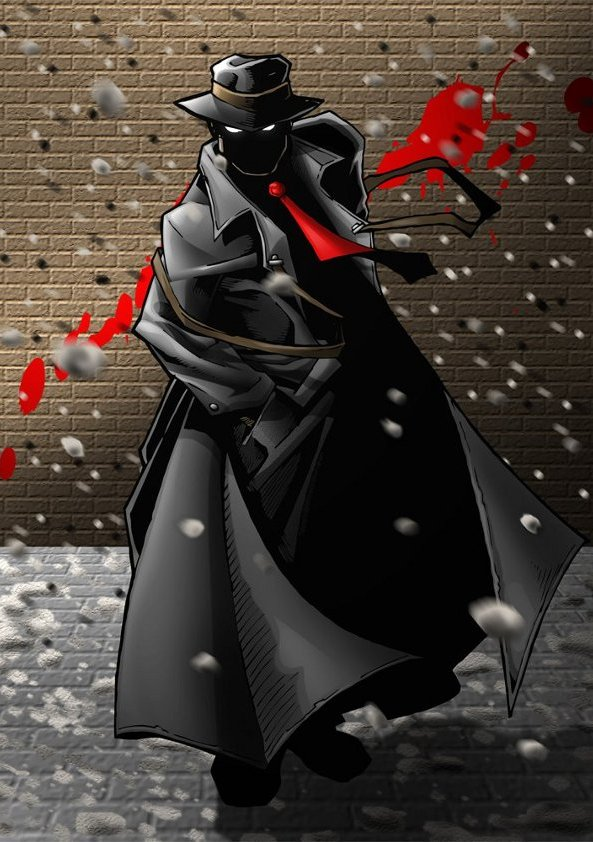
\includegraphics[width=\paperwidth,height=\paperheight]{images/cover}}
\begin{center}
    \color{white}\vspace*{\stretch{1}}

    \textbf{\fontsize{60}{72}\selectfont\itshape\thetitle}\vspace{1.5\baselineskip}

    \rule{0.5\textwidth}{3pt}\vspace{0.5\baselineskip}

    \textbf{\LARGE\theauthor}\vspace*{\stretch{1}}

    \large\theeditorial
\end{center}

\endinput

\newpage\pagecolor{white}

\frontmatter
\thispagestyle{empty}
\hbox{}\newpage
\thispagestyle{empty}
\vspace*{\stretch{1}}\noindent
\textbf{\titlename}\\
\authorname

\footnotesize

\bigskip\bigskip\noindent
\textbf{\copyright\ 2010--2011, \authorname}\\
\textbf{\copyright\ 2011, de la edición, \editorname}\\
Se otorga el permiso para copiar, publicar y/o distribuir libremente esta obra y/u obras derivadas de esta obra, ya sea total o parcialmente, por cualquier medio y con cualquier propósito sin ánimo de lucro, siempre y cuando esta nota se mantenga.\\
{\fontencoding{OT1}\fontfamily{cmr}\selectfont\url{http://creativecommons.org/licenses/by-nc-sa/3.0/es/}}

\normalsize

\noindent\ccbyncsaeu

\footnotesize

\bigskip\noindent
\textbf{Edición:} \editorname\\
Realizada íntegramente con \emph{software libre}, mediante el procesador \LaTeXe\\
\Letter\ {\fontencoding{OT1}\fontfamily{cmr}\selectfont\href{mailto:xoansampainho@gmail.com}{\nolinkurl{xoansampainho@gmail.com}}}\\
\Telefon\ \href{tel:+34620194971}{+34 620194971}

\bigskip\noindent
Impreso en la Red. \emph{Printed in Internet}

\normalsize

\endinput


\maketitle

\cleardoublepage
\raggedcolumns
\tableofcontents
\flushcolumns

\mainmatter
\setcounter{chapter}{24}
\addtocontents{toc}{\protect\vspace{0.5\cftbeforechapskip}\protect\begin{multicols}{2}}
\chapter{Plan oculto}
Muchas preguntas ya tenían respuesta. Pero al mismo tiempo, nuevas incógnitas salían a la luz. Misterios que hacían tambalearse la estructura misma de la organización y arrojaban nuevas y sorprendentes pistas sobre su origen.
Y gran parte de esas respuestas estaban en manos del que había sido hasta ese momento su enemigo parapetado en el anonimato\dots

\fancyparbreak
Sam Grove le dijo que no se lo creería cuando lo supiera. No se hacía una idea de cuánta razón tenía.

El Juez Nitram y Starr Miles, aliados. Amigos. O al menos, algo muy similar. Las circunstancias concretas de esa relación eran aún desconocidas para ellos, pero sin duda distaban mucho de ser de naturaleza meramente casual. La justicia había movido los actos de aquellos dos hombres desde antes que él mismo pusiera los pies sobre una nave espacial. Eran perros viejos en un mundo más viejo aún.

Y ahora el pasado regresaba para ponerlo todo a prueba. Establecer la duda, la incertidumbre sobre en qué han estado basando realmente todo aquello que han construido. Quién era realmente Starr Miles. Él mismo decía que el pasado no importaba, sólo el presente. Pero lo que por aquel entonces era el presente ya se había convertido en el pasado para todos ellos.

Ya habría tiempo de indagar en detalle sobre lo que acababa de salir a la luz, por otro lado. Era el momento de la acción. De atacar con fuerza, rapidez y contundencia.

Como Echo había anticipado, los suyos no habían perdido el tiempo en su ausencia. Ya tenían los datos de la inmensa mansión en la que Nitram se había retirado, un lugar que al parecer ocupaba de manera habitual para alejarse de las cámaras que atormentaban a otros jueces y otras personalidades públicas. No había cifras exactas, pero la mansión podía estar fácilmente vigilada por treinta o cuarenta guardaespaldas, y eso sin contar con torretas de seguridad en pasillos y puntos muertos.

El concierto de The Jammers no había empezado aún, además. Grove estaba allí, infiltrado entre el público, esperando dar la buena noticia de que las comunicaciones se habían restablecido de la manera más clara posible: usando como prueba el propio mensaje enviado. Su escuadrón también estaría por los alrededores, de modo que se pudiera restablecer la normalidad en la medida de lo posible.

Según los datos de Razorclaw habían sucumbido veinticuatro hombres en las calles desde el comienzo de la vendetta. Diez habían sido descubiertos por cazarrecompensas y obligados a fingir ser imitadores, cinco habían sacrificado su puesto para llamar la atención de manera voluntaria y añadir confusión a los casos anteriores, cinco habían sido heridos de gravedad y dos parejas habían muerto, una de ellas a causa de las letales heridas y otra al autoinmolarse para proteger el secreto.

En total, la organización había perdido a la cuarta parte de sus componentes, pero tendrían que aprender a surgir de las cenizas. Lo primero de todo sería que no se ampliaría la formación. Casi todos los que habían muerto eran novatos, y no se perdonaría que algo así pudiera pasar de nuevo. Aquella experiencia le había enseñado que, si bien eran un equipo, cada hombre tenía que estar sobradamente preparado para actuar como si estuviera solo frente a todas las adversidades existentes en el mundo.

De todos modos, Los Caídos no podrían ser de mucha ayuda en el asalto al interior de la casa. Dado que las comunicaciones aún no se habían restablecido, lo que harían sería asegurar el exterior y los alrededores y dejar la parte de la infiltración a él y los cazarrecompensas, más que ansiosos por llegar hasta el epicentro del asunto.

Cuando se reunió con ellos comprobó que, pese a que Krexon se había escabullido, no habían estado perdiendo el tiempo precisamente. El socio de Dobleseis, Códec, tenía un buen arsenal que no habían desaprovechado en lo más mínimo, y pudo comprobar cómo estaban armados hasta los dientes con toda clase de lanzarrayos, gran parte de potencia no letal, pero muchos otros, pensados para las defensas automáticas, más que demoledores.

Dobleseis, sin embargo, apenas cogió armas. Estaba extasiado con su juguete nuevo, y planeaba toda clase de maniobras que realizar a dos manos con aquellos revólveres multiusos. Scream no quería ni pensar qué hubiera podido hacer Silenciador en su momento si hubiera tenido la capacidad del cazarrecompensas para poder dividir su concentración y puntería con simétrica eficacia.

Los cazarrecompensas, dentro del hecho de que eran tipos que actuaban por separado, se habían logrado compenetrar bastante bien. La planificación fue sencilla, rápida y ágil. No había sitio a las sutilezas en aquella ocasión. Además, la improvisación sería una parte esencial del ataque. Gracias a Saw, que había estado dentro de aquella casa en el pasado, cuando trabajaba para Gorgon, conocían el emplazamiento de los lugares más importantes de la misma, pero la disposición, en mayor o menor medida, podía haber cambiado.

La mansión disponía de tres plantas y estaba realizada en estilo precolonial, con una fachada adornada con complicadas escalinatas y columnas de orden corintio. Los ventanales poseían amplios dinteles, pero el blindaje de los cristales era muy resistente y difícil de atravesar. El techo permanecía también bajo vigilancia, y en términos globales el lugar apenas tenía entradas secundarias de tipo alguno, pues el garaje era subterráneo y se accedía desde un pasadizo situado muchos metros atrás. En su momento, de hecho, se intentó conectar una de las entradas del Aquerón con el interior de la mansión, pero resultó a todas luces imposible, si bien Scream no dudaba que la cantidad de pasillos secretos que debía poseer aquel lugar sin duda sería más que considerable dada su importancia política.

De todos modos, aunque no hubiera una entrada, no hubo problemas al respecto. Repulsor no tardó en fabricar una, tratando de calibrar al máximo el disparo para así no suponer un peso muerto una vez lo hubiera generado.

Los primeros en pasar fueron Dobleseis, Silencio y el propio Scream. Barrera cubriría a Repulsor, y Batería estaba al cargo de hacer que se recuperara cuanto antes, así como recargar de nuevo su equipo al completo. Fue por ello que obviamente se quedaron atrás en comparación con sus más veloces compañeros, que salieron disparados escaleras arriba para ganar una planta antes de que la movilización y la confusión les obligaran a pelear por cada palmo que recorrieran hacia la estancia principal, donde suponían que estaría Nitram, tal vez incluso esperándoles.

Las primeras defensas se cruzaron en el camino de los tres furtivos, y Dobleseis las despachó de un par de tiros sin dejarlas siquiera realinearse. Por desgracia la cosa empezó a ponerse al rojo vivo, y no tardaron en encontrarse con cinco hombres que les cortaban el paso. La batería de disparos fue encarnizada, pero uno por uno lograron derribarles, derrotando Scream a uno de ellos, Dobleseis a tres y Silencio al último, una vez logró colocarse a su espalda.

~---Perfecto, mudito ~---fue la única respuesta de Dobleseis. Silencio se acercó de nuevo a ellos, su actitud tranquila y pausada, evaluando la situación. Sin embargo de repente, sin previo aviso, apartó a Dobleseis de un golpe y recibió una descarga de una de las defensas automáticas abatidas, que había disparado con parte de energía residual que había logrado acumular.

El disparo no era fatal, pero el disparado estaba muy malherido. Dobleseis se quedó mirando, sin saber qué decir. Era la primera vez desde que era cazarrecompensas que alguien recibía de manera voluntaria un tiro en su lugar. Como única respuesta, frió la torreta con un disparo de sobrada potencia procedente de una de las antiguas armas del peor enemigo de Reflector.

Silencio les miró y les hizo un gesto para que continuaran.

~---¿Estarás bien? ~---preguntó Scream.

Escucharon ruido de disparos al fondo, y supieron que se trataba de sus compañeros rezagados. Silencio se limitó a hacer un gesto con la mano abierta para que se marcharan. No había que ser ningún lince para deducir que se ocultaría hasta que ellos alcanzaran su posición.

~---De acuerdo, seguiremos entonces.

Dobleseis y Scream prosiguieron a lo largo del pasillo, y si bien se encontraron con otros guardaespaldas por el camino, quedó claro que el grueso de la artillería ya había sido lanzado ya, algo más lógico que ir aumentando de manera escalonada la dificultad de los oponentes a medida que llegaban a su objetivo. Las defensas no supusieron problemas tampoco, aunque habían recalibrado su puntería en función de los movimientos de sus blancos y resultaba más complicado esquivar sus disparos, sobre todo para Scream, que confiaba más en engañarlas con sus dispositivos y hacer que sus rastreos de imagen, calor y cinética se confundieran para dispararse entre ellas.

~---Ingenioso ~---se limitó a decir Dobleseis al tiempo que recargaba sus cuatro lanzarrayos, con sus respectivas bocas humeantes y rojizas.

Ante ellos se alzaba la puerta de doble batiente que les separaba del despacho en el que sin duda se hallaba el Juez. Scream hubiera optado por una entrada pausada, solemne, dejar que las puertas se abrieran con lentitud para después proyectar una silueta anormalmente grande escurriéndose por los pliegues de luz del suelo.

Dobleseis se limitó a echarlas debajo de una patada en lo que tenía listos y preparados los seis gatillos de sus armas.

El Juez Nitram estaba ante ellos, al otro lado de un pulido escritorio de roble, en una sala con una fastuosa decoración heredera de tiempos extintos. Llevaba un traje negro de corte antiguo, y tenía una mano en el bolsillo mientras la otra se apoyaba en el respaldo de la silla, tan arcaica como el resto del mobiliario.

Dobleseis no dudó ni siquiera un segundo. Descargó los cuatro lanzarrayos directos hacia el Juez. Sin embargo cuatro discos salieron de detrás del escritorio, veloces como insectos enfurecidos, y se interpusieron en la trayectoria de los disparos. Los otros seis no tardaron en mostrarse también a la vista de los asaltantes.

~---Es de sujetos como usted de lo que estas máquinas me protegen ~---apuntó Nitram, indiferente, como si no estuviera hablando en persona con ellos sino a través de una pantalla~---. Pero toda precaución es poca ~---acabó apretando un botón del escritorio, justo después de que sus discos avanzaran algo más de medio metro de distancia, lo que hizo que Dobleseis y Scream se alejaran hasta una pared cercana con una estantería llena de libros. Ninguno de los dos notó nada extraño, pero estaba claro que había activado alguna clase de protección invisible, tal vez energética.

\emph{Se acabó, Juez Nitram. Será cuestión de tiempo que lleguen los otros y se unan a la pelea.}

~---Eso no es problema para mis ayudantes ~---dijo señalando a los discos con un gesto de la palma abierta~---. Sus circuitos tienen bien integrados todos los trucos de estos mercenarios.

~---¿Qué es lo que quiere de los cazarrecompensas? ~---preguntó Dobleseis~---. ¿Exterminarnos? ¿Inculparnos y encerrarnos?

~---Aunque así fuera, aunque considerara que son la escoria de la sociedad, no procedería de tal manera, pues ahora sirven a un bien mayor, un objetivo mucho más honorable que perseguir delincuentes y matones por una despreciable suma de dinero. Ahora son parte de un gran plan, una estrategia global.

\emph{¿Tiene algo que ver ese plan con Starr Miles?}

Nitram miró a Scream, lleno de asombro. Al parecer, dedujo, no sólo ellos buscaban respuestas concretas a preguntas complejas.

~---De modo que mi sospecha era cierta ~---comentó~---. Miles está detrás de ti, de tu creación. Eso no hace más que confirmar la utilidad de todo lo que ha estado pasando.

\emph{¿Qué buscaba con todo lo sucedido?}

~---¿Acaso no lo sabes? Pensé que al menos tú, que pareces tener sobradas aptitudes para la investigación, acabarías por averiguarlo. Miles y yo teníamos objetivos comunes, buscábamos alcanzar un mismo fin: la forja de un ser especial, único. Aunque con fines muy distintos, claro, tan distintos como nuestras respectivas personalidades. En el caso de Miles, él estaba obsesionado con la justicia, con encontrar una figura que impusiera respeto, miedo y obediencia.

»En mi caso, buscaba comenzar la Purga.

Dobleseis y Scream miraron fijamente a aquel hombrecillo en apariencia inofensivo, de no haber sido por esos discos endiablados que flotaban por delante de su cuerpo. En sus ojos se reflejó un brillo de malevolencia insondable e infinita.

~---¿A qué se refiere? ¿Un alzamiento?

\emph{No} ~---dijo Scream, encogiendo los hombros~---. \emph{Religión. Un advenimiento.}

~---Parece que sí eres una creación de Miles después de todo, y al menos estás bien informado ~---fue el único comentario de Nitram.

\emph{La Purga} ~---explicó Scream a Dobleseis, pero sin dejar de mirar a su enemigo común~--- \emph{es una vieja creencia de los Gilock. Ellos creen que vendrá un superser, o algo similar, que traerá una nueva era al Universo, que acabará con la corrupción y el caos. Que se enfrentará a otros similares a él, pero inferiores en realidad, y los exterminará, para convertirse en el único y verdadero, aquel cuyos designios todos seguirán, por ser éstos justos y auténticos.}

~---Explicado de manera tosca y simple, así es ~---apuntó Nitram.

~---De modo que por eso traernos aquí, enfrentarnos los unos a los otros, montar un torneo por toda la ciudad\dots\ para que sólo quedara el mejor.

~---Así es, cazarrecompensas. Mis intereses se habían puesto en el Caído, y por eso puse una recompensa por su cabeza. Una vez lo derrotaste, dejó de tener interés para mí, y tú pasaste a ser mi objetivo.

\emph{Por eso interfirió las comunicaciones, para impedir que los cazadores se informaran entre ellos y no pudieran hacer equipo.}

~---En efecto.

\emph{No ha funcionado, Juez. Nos hemos rebelado, y su experimento ya no tiene éxito.}

~---Eso es lo que crees, ¿no? Pero la mente de los seres es voluble, y sus intenciones son maleables. Demuéstraselo, ya ~---ordenó Nitram, sin que Scream supiera a quién se estaba dirigiendo.

No tardó en averiguarlo cuanto unos brazos violáceos surgieron de la pared para agarrar a Dobleseis del cuello y apuntar a su cabeza con un láser.

~---Volvemos a vernos ~---dijo Krexon guiñando los ojos.

~---Como puedes ver, ahora mismo tengo al cazarrecompensas en mi mano. Hay una gran suma aún en pie para quien me lo traiga vivo. Está inmovilizado, quieto. Si mueve un músculo, es hombre muerto. Ah, ya vienen ~---dijo Nitram escuchando alboroto en el pasillo~---. Justo a tiempo.

Los otros cazadores irrumpieron en la sala y cruzaron las puertas aún abiertas para colarse en su interior. Silencio estaba apoyado en el hombro de Batería, pero no había soltado las armas ni tenía intención de hacerlo, y Batería, además de sus propias pistolas recargables, portaba en la cintura unas granadas de pulso eléctrico que después de pasar por sus manos podían resultar como poco devastadoras. Barrera llevaba a la espalda un rifle de asalto militar, y Repulsor sostenía una de las defensas de la propia casa que había arrancado de cuajo para usar de improvisada arma automática a dos manos.

~---Tú eres el que está detrás de todo esto, ¿verdad? ~---preguntó Repulsor sin demasiada cortesía.

~---Escucha atentamente, pues te interesa lo que voy a decir, y vosotros también. A partir de ahora retiro la recompensa por todos vosotros, y sólo la ofrezco por ese justiciero de ahí ~---señaló a Scream~---. Nueve millones si acabáis con él. Tocáis a más de dos millones por cabeza.

~---Juez, ¿sigue estando en pie la recompensa por esta araña humana? ~---preguntó Krexon, aún con su presa entre los brazos.

~---Así es, Krexon. No prometo en vano cuando ofrezco algo, y habrás sacado a un forajido de las calles.

Los demás cazarrecompensas no dijeron nada. Parecía claro que no iban a aceptar la propuesta, pero hubo un momento de silencio, como si cada uno de ellos esperara que fuera otro el que dijera la primera palabra de rechazo al respecto. Scream, sin embargo, no tenía en ese momento la atención puesta en ellos sino en el incorpóreo y viscoso alienígena.

\emph{Te ha utilizado, Krexon. Como a todos nosotros. ¿Por qué crees que no ha puesto un precio por ti?}

~---Porque colaboro con él, estúpido ~---replicó el alien con desprecio.

\emph{Eso sólo es parte de la verdad. Ya hace tiempo que te derroté, y él lo sabe. Por eso ya no formas parte de su plan. Tú no eres el elegido que busca. ¿Sabías que fue embajador de los Gilock?}

Los demás presentes, incluido Nitram, no dijeron nada. No sabían qué quería decir con todo aquello.

~---¿Los Gilock?

\emph{Los Gilock, sí. Creo que los Axcronianos tuvieron más que palabras con ellos en el pasado, ¿verdad? Los planetas de ambas especies quedaban bastante cerca, en el mismo sistema, ¿no es así, Juez?}

El Juez no respondió, pero un atisbo de ira empezaba a aflorar en su interior.

\emph{Un sistema binario, si no me equivoco. Y mientras que tu especie evolucionó para que al volverse incorpórea pudieran sobrevivir a las constantes lluvias de meteoritos, los Gilock optaron por desviarlos. Desviarlos, Krexon.}

\rquoti Dime, Krexon, los tuyos no lograron predecir la llegada del meteorito que los fulminó, ¿verdad? Como si su comportamiento no fuera el esperado según su trayectoria inicial, ¿o no?

~---¡Basta! ~---fue la única palabra que pronunció Nitram antes de lanzar sus discos flotantes contra Scream, que a duras penas lograba esquivarlos, engañándolos por medio de ilusiones ópticas. El grupo de cazarrecompensas asistía, insólito, a poco menos que una acusación velada de genocidio por parte de una especie hacia otra de su mismo sistema.

~---¿Usted lo sabía, Juez? ~---dijo Krexon, soltando la presa de Dobleseis, quien al instante, furioso, trató de derribarle, pero sus puños le atravesaron como si fuera un fantasma~---. ¿Es cierto lo que dice?

~---Deberías sentirse orgulloso, Axcroniano. Fuiste elegido, sé que te consideraron el único digno de aspirar a pasar la primera fase de la Purga en tu planeta. Otros que como tú no estaban en él en ese momento no fueron tan afortunados.

~---Morirá por lo que acaba de decir y ninguno de sus aparatos podrá impedírmelo ~---fue el contundente comentario del alienígena, caminando directo hacia el Juez.

El invisible campo de baja frecuencia que estaba entre ellos, sin embargo, le impidió dar un solo paso más hacia la consecución de su objetivo.

Los Axcronianos no podían atravesar ciertas energías, y eso era algo que, como antiguo embajador de los Gilock, el Juez Nitram sabía bien. Por eso, la defensa que había bajado tras la aparición de Dobleseis y Scream, más que para detenerles a ellos, servía de cara a obtener una potencial defensa contra su subalterno aún escondido.

Krexon comenzó a convulsionarse como si le hubieran dado una sacudida de miles de voltios, y cayó al suelo echando humo y emanando un olor como ningún otro que los presentes hubieran percibido antes. Estaba aún vivo, pero desde luego también fuera de combate por un tiempo prolongado.

~---Mira lo que me has obligado a hacer ~---dijo Nitram mirando a su peón caído~---. Te mataré por eso.

~---Me temo que no, amigo ~---replicó Repulsor apuntando hacia los discos de Nitram con toda su potencia~---. Ya hemos visto lo que vale tu palabra con bastante claridad.

~---Insensatos ~---continuó Nitram, enfurecido~---. No sabéis lo que estáis haciendo. Estos discos son la cumbre de la tecnología de los Gilock, y pueden enfrentarse contra ejércitos enteros.

~---Ya lo veremos ~---dijo Dobleseis disparando la red electrificada de uno de los revólveres de Silenciador y atrapando a cuatro de ellos en la misma.

~---Esa red no vale de nada, cazador. Su energía no basta para detener a mis máquinas. Deberías haber supuesto que estaría preparado para esa posibilidad.

~---Habrá que usar la recámara, entonces ~---terminó Dobleseis sacando el segundo revólver.

~---¿Otro arma? ~---comentó Nitram~---. Da igual, aun teniendo este imprevisto en cuenta, ni con una descarga doble podrías dañarlos.

~---¿Y qué tal si la descarga es mayor? ~---añadió Batería tocando el arma justo antes de que Silenciador disparara. Una segunda red de energía concentrada, capaz de freír a cualquiera que entrara en contacto con ella, cayó sobre los discos atrapados y al soltar toda su potencia sobre ellos los dejó tan inservibles que apenas eran capaces de separarse malamente unos centímetros del suelo.

~---Pagarás por eso ~---fueron las únicas palabras de Nitram antes de lanzar a sus restantes discos contra ellos.

En teoría era una pelea justa. Eran seis, y quedaban seis de aquellos cacharros. Sin embargo, aunque pomposas en exceso, las palabras de Nitram no estaban ausentes de verdad. Algunos de los presentes, como Batería y Silencio, no eran rivales frente a aquellos instrumentos de tortura flotantes, y pronto otros más poderosos como Dobleseis o Barrera tuvieron que probar ración doble del enemigo. Repulsor era incapaz de atinar a unos objetivos tan escurridizos, y Scream poco podía hacer más que evitar que le impactaran, un baile que podía estar manteniendo durante bastante tiempo, pero no eternamente.

Sólo Dobleseis parecía tener alguna ligera ventaja frente a los chismes flotantes de Nitram, pero aunque logró igualar un poco la balanza, pronto todos ellos estuvieron o bien en el suelo, o bien arrinconados contra alguna pared. Más de uno deseó en ese momento haber pertenecido a la raza de Krexon, fuera de combate sin posibilidad de despertar a corto plazo.

~---Se acabó, cazarrecompensas. Última oportunidad de pelear entre vosotros en pro de un bien mayor para el Universo.

\emph{Si tanto buscas a un ser último y definitivo, ¿por qué no te ofreces para el puesto?} ~---argumentó Dobleseis con cierta ironía.

~---No he sido yo quien os ha derrotado. Cualquiera con estos discos en su poder podría haberlo hecho, aunque sólo yo los poseo entre toda la humanidad. No, una vez que el verdadero poder del vencedor despierte, será una fuerza contra la que nadie nada podrá hacer. En todo caso, está claro que no sois ninguno de vosotros, y no vais a colaborar bajo ninguna circunstancia. Da igual, aún quedan muchos otros cazarrecompensas en la ciudad.

De repente Scream notó un ruido familiar en uno de los bolsillos de su gabardina. Era un ruido que llevaba tiempo sin escuchar, y que había aprendido a valorar como el más preciado de los tesoros. La estática de su comunicador, mal configurado por descuido y la falta de uso.

Apretó el botón disimuladamente, de modo que nadie le viera hacerlo, y escuchó la voz de Sam Grove, llena con la sensación de júbilo y regocijo propia del deber cumplido.

~---Capitán, hace tiempo que acabaron, pero las comunicaciones han tardado un tiempo el volver. ¡Capitán! ¿Me oye?

Scream no contestó. Sólo tenía ojos para el disco que flotaba a la altura de su cabeza, con un láser colocándose en línea con su rostro.

~---¡Capitán, ellos están allí!

Casi al momento de que Grove terminara de hablar, el disco empezó a emitir una serie de extraños brillos y cayó al suelo, como si se hubiera cortocircuitado.

Al otro lado de la puerta, seguido del resto de su grupo, Scream pudo ver a Distorsión estirando la mano hacia el aparato.

~---Tú nos contrataste, ¿verdad? ~---fueron sus palabras, señalando a Nitram~---. Puedes considerar nuestro acuerdo liquidado.

Nitram no se molestó en contestar aquellas palabras y se limitó a lanzar el resto de sus discos contra The Jammers. Sin embargo aquellas máquinas no eran rivales contra el alcance de sus poderes, y enseguida los otros discos acabaron girando sobre sí mismos, moviéndose con aparatosa lentitud, cayendo al suelo casi drenados de energía o disparándose los unos a los otros al rebotar sus láseres en la componente femenina del grupo.

\emph{Se acabó, Juez} ~---dijo Scream levantándose~---. \emph{Las comunicaciones han regresado, su experimento ha fallado.}

~---Sólo por ahora. Sólo por ahora. Pero nada podéis hacerme. La inmunidad de mi cargo me protege.

~---Veamos si puede protegerle de esto ~---dijo Dobleseis disparando cuatro descargas de láser hacia Nitram, pero el campo de fuerza que abatió a Krexon las absorbió tras combarse ligeramente y demostrar así su presencia invisible.

~---Adiós, cazadores ~---terminó el Juez Nitram, marchándose por una puerta que había en su lado de la sala. Al poco rato los discos comenzaron a levantarse, unos más aparatosamente que otros, y salieron volando pasillo abajo, sin que fuera posible atinarlos o detenerlos.

~---Son aparatos impresionantes si han logrado que mi amigo dedos rápidos no logre apagarlos por completo ~---dijo Distorsión mirando a Overdrive.

\emph{Gracias por la ayuda} ~---agregó Scream levantándose, al tiempo que los cazarrecompensas se incorporaban también.

~---¿Amigos tuyos? ~---preguntó Distorsión como si acabara de hacer el comentario más normal del mundo en el momento más propicio para el mismo.

\emph{Dejémoslo así.}

~---Bien, con esto nosotros hemos cumplido. La próxima vez, nos andaremos con cuidado y no nos volveremos a fiar de desconocidos.

~---¿Sois cazarrecompensas? ~---preguntó Dobleseis.

~---¿No sabes quienes somos? ~---dijo Distorsión, con sincera sorpresa.

~---No ~---fue la escueta respuesta del multibrazos.

~---Permíteme, entonces ~---dijo acercándole un par de entradas que tenía en el bolsillo~---. Son para nuestro próximo concierto en la colonia de Bludgor, por si\dots

Antes siquiera de que acabara de hablar, el cazarrecompensas ya estaba reduciendo a pedacitos las dos entradas.

~---Supongo que no te interesa mucho la música.

~---El único ruido que me interesa es el que yo genero ~---contestó mostrando los lanzarrayos.

Scream recibió un mensaje de radio donde le decían que tenían que salir de allí cuanto antes, pues la policía se acercaba a acordonar la zona. Al fin habían vuelto los buenos viejos tiempos, pensó.

\emph{Por éste no dan una recompensa} ~---dijo señalando a Krexon~---, \emph{pero espero poder confiar en vosotros para que lo entreguéis a las autoridades.}

~---Descuida ~---comentó Repulsor~---. De hecho Silencio, Barrera y yo estuvimos hablando y estábamos considerando asociarnos. Habíamos pensado como nombre Fortaleza, ¿qué te parece?

\emph{Pensadlo un poco más} ~---contestó con sinceridad Scream.

~---¿Qué hay de ti, vieja gloria? ¿Tú y Códec os uniríais a nosotros?

~---No, gracias. Demasiado a repartir ~---dijo Dobleseis saliendo de la habitación y marchándose pasillo abajo.

~---¿Siempre es así de amigable? ~---preguntó Distorsión~---. Por cierto, ¿os interesa a vosotros venir a algún concierto de nuestra gira? Es lo menos a cambio de todas las molestias que hemos causado.

~---¿Qué edad tienes, hijo?

~---Eso no importa, abuelo. ¿Le interesa o no?

~---No, no me interesa. Si todavía fuerais Balamb Garden\dots\ esos sí que eran buenos, y muy legales cuando los conocí, en sentido figurado, claro.

~---¿Conoció a Balamb Garden? ~---preguntó Echo impresionada, subiéndose la visera, distinta a la de unas horas antes y dedicada al grupo Garbage.

~---Antes de que tú nacieras, muchacha ~---contestó Repulsor mientras todos se marchaban pasillo abajo, con el ruido de fondo de las sirenas de los deslizadores patrulla.

\parbreak
Como era de esperar, el Juez Nitram declaró que había sufrido un intento de atentado frustrado en su propia residencia temporal. Como era de esperar también, cuando le preguntaron por el aspecto de sus atacantes no recordaba del todo bien cuál era éste, y algo similar le pasaba al resto de sus guardaespaldas. El asunto había quedado como parte de una guerra secreta. Las recompensas se retiraron oficialmente sin que la opinión pública supiera quién las había emitido. Krexon fue el único arrestado, y su presencia sospechosa en el lugar del asalto bastó para realizar un estudio más severo de su caso, además de recluirle en un régimen especial. Su colaboración con las autoridades fue nula, por decir que colaboró de alguna manera. El único tema que parecía producirle algo de interés era la extinción de su especie, y siempre parecía a punto de tener la intención de añadir algo al respecto, pero no tardaba en caer de nuevo en el hermetismo y limitarse a abrir y cerrar por turnos sus ojos dispersos alrededor del rostro.

Los Caídos volvieron a reorganizarse y realizar un informe de daños. La vorágine de aquellos días hizo que se olvidara temporalmente al Caído, aunque no tardaron en señalarle como culpable indirecto de la afluencia de cazadores de bonificaciones en las calles de la ciudad. De todos modos, no era nada por lo que no hubieran pasado antes.

John Scream no tardó en volver a sus ocupaciones habituales, aunque de vez en cuando se permitía unos segundos de solitaria reflexión. En uno de ellos le cogió Sky un día, efectuando una visita sorpresa a Gorgon Enterprises, donde Scream estaba realizando bocetos preliminares de prototipos destinados al año siguiente.

~---Ha ido de poco, por lo que me han contado.

~---Así es. Esta vez hemos estado cerca de ser descubiertos. Pero el Juez Nitram no sabía nuestra verdadera naturaleza. Cree que somos uno, aunque tiene una pieza del rompecabezas que puede llevarle a averiguar la verdad.

~---De modo que conocía a Miles. Quién sabe qué clase de relación se había forjado entre ellos dos\dots\ tal vez fueron enemigos, amigos sinceros, o incluso aliados en la lucha contra el crimen.

~---Puede que nunca lo sepamos. Y aunque lo hagamos, hasta entonces la única persona que nos podía ayudar a entender mejor a nuestro mentor es, por desgracia, uno de nuestros más declarados enemigos ~---terminó Scream llevándose la mano a la boca, en actitud reflexiva.


\chapter{Torneo \emph{\mdseries(Parte 1)}}
La persecución a la que habían sido sometidos había terminado, pero siempre había algo de lo que preocuparse en aquella ciudad. Nuevas situaciones, nuevos conflictos. Y no en todas las ocasiones de naturaleza criminal.

En realidad era la sombra de los tiempos pasados lo que en breve tendrían que afrontar, en más sentidos de los que imaginaban\dots

\fancyparbreak
Las semanas habían pasado y las comunicaciones habían sido restablecidas en su práctica totalidad a lo largo de las cenicientas calles de Ernépolis. No en todas partes a idéntica velocidad, claro. En aquellos barrios donde se concentraba una mayor renta media fueron revisadas con mayor celeridad que en las zonas más deprimidas, como podían ser los Túneles o en general todo el sector Sur. Se trataba de una forma de corrupción leve, no demasiado fatal para el destino de la población, pero prueba presente de que incluso en las más pequeñas acciones la influencia del poder permanecía latente y operante a las acciones de los ciudadanos.

Como resultado del fallo generalizado de transmisión, que nunca fue del todo esclarecido, aunque se creyó que tuvo que ver con alguno de los múltiples cazarrecompensas que visitaron la ciudad, se procedió a una revisión completa de todas las instalaciones con el fin de reforzar su seguridad contra ese tipo de ataques. Tal acción, modificar toda la infraestructura eléctrica de Ernépolis, en muchos casos vieja y corroída por efecto de la dejadez y el adverso clima, trajo consigo numerosas consecuencias en términos de obras públicas.

Las calles y callejones se llenaron de socavones. Agujeros enormes, del tamaño de vehículos deslizantes en muchos casos, empezaron a dominar el paisaje urbano allá donde se posara la mirada. Además de eso, era habitual tener que efectuar cortes ocasionales en otras infraestructuras.

La más afectada e importante fue, sin lugar a dudas, la instalación lumínica. Era habitual que, fuera de los horarios laborales, barrios enteros se quedaran casi sin luz, con unos escasos focos de emergencia que, unidos a la Nube eterna que siempre secuestraba el ya de por sí escaso brillo lunar, retrotraían a la ciudad a tiempos en los que las tinieblas eran aún más poderosas de lo que solían ser en la época actual.

Muchos pensaban en el Caído y en su regocijo no sólo por haber escapado del acoso al que había sido sometido, sino también al comprobar que la ciudad era cada vez más territorio de la penumbra, un juguete nuevo para sus siniestros designios.

Nada más lejos de la realidad. Para Los Caídos las tinieblas eran un medio. Pero nunca, jamás, serían un fin, y eso era algo que Scream siempre tuvo claro desde que entró en la organización. Ser parte de la oscuridad, fundirte con ella. Pero no confundirte en ella, perder la personalidad. Ese era el error que por regla general acababan cometiendo muchos de los justicieros tenebrosos de antaño.

Era el tiempo para la reflexión en la quietud de su pequeño despacho del Aquerón, un lugar casi inaudito teniendo en cuenta la imagen de inhumanidad que ofrecían de cara al exterior. La lista de enemigos que poseían era ya, cuanto menos, importante y a tener en cuenta. Había monstruos, tanto física como psicológicamente hablando, y también déspotas y tiranos, sujetos que se creían superiores a todo y todos y con la capacidad para decidir por los demás. Unos se movían por poder, otros por odio, y también por ideales, incluso. Por supuesto no faltaban los enemigos de la vieja escuela, los que buscaban dinero o fama. Y eso sin contar toda una serie de personajes de ambiguo comportamiento y complicadas reacciones de cara al futuro.

Entre esos, estaba el desaparecido Starr Miles.

Scream no había dejado de pensar en ello desde que supiera que él y Nitram se conocieron en el pasado. Tal vez la organización no había empezado tan de cero como pensaban en un principio. Puede que Miles ya hubiera hecho antes pruebas, experimentos. O llegado a pactos que no les gustaría conocer.

En todo caso, algún día acabaría por averiguar las respuestas a esa clase de preguntas. El Juez Nitram había salido indemne por completo del asalto a la mansión, como no podía ser menos dada su posición oficial, mientras que unos peones fueron encarcelados, como Krexon, y otros se retiraron de la partida con el objetivo de no volver a ella jamás, como la mayor parte de los cazarrecompensas.

Sin embargo aquel no era el asunto más inmediato que requiriera su atención. La extraña novedad había surgido con las noticias que Saw le traía, jugosas y recién proclamadas, aunque no tardarían en ser difundidas.

~---¿Dices que el Presidente Scatter busca aspirantes a protectores de la ciudad? ~---comentó levantando la vista de los informes del día de los escuadrones.

~---Así es, John. A mí también me costó creerlo cuando me comunicó su idea de manera personalizada.

~---¿Crees que alguien puede haberle\dots\ sugerido tal eventualidad?

~---No lo sé. Aunque paso con él la mayor parte del tiempo que no estoy aquí, se mantiene en permanente contacto con toda clase de estratos de poder en la ciudad, y algunos de ellos son enemigos declarados nuestros.

~---En todo caso, sea como fuera la manera en que se le ha ocurrido esta idea, lo que está claro es que no puede traer nada bueno para nuestra estrategia. Puede que quieran volver a ir a por nosotros, o quién sabe qué puede pasar. Además de eso la ciudad se llenará de novatos inexpertos que puede que se pongan en peligro a sí mismos y a otros con ellos\dots\ y eso sólo en el mejor de los casos.

~---Piensa ser lo más cuidadoso posible al respecto de eso, pero al mismo tiempo pretende volverse todo lo políticamente correcto que la situación le permita. Creo que quiere pasar a la historia como el Presidente que reinstauró el orden en la ciudad con nuevos símbolos de justicia.

~---Un héroe estatal\dots\ un policía con poderes.

~---No es algo que nos suene del todo desconocido, si lo pensamos un momento ~---observó Saw.

~---Creo que esto no va a gustarle demasiado a Sky, si le conozco lo suficiente.

~---Yo también lo creo.

~---Mantenme informado de todo lo relacionado con este asunto. No te preocupes por tus tareas como jefe de escuadrón, alguien os sustituirá. Este asunto tiene prioridad al menos hasta que esclarezcamos exactamente qué clase de espectáculo pretende el Presidente montar y presentar.

~---Así lo haré, descuida.

Saw salió del despacho y se quedó un momento reflexionando. No le gustaría estar en el pellejo de Scream, pensó con frialdad. Siempre tenía que mostrar la máxima preocupación ante cualquier cosa que ocurriera en la ciudad, incluso hechos que podían luego no trascender en nada importante, como era ese concurso, esa suerte de oposición a héroe que tal vez se quedara en saco roto.

 

Al día siguiente, a primera hora de la mañana, con las luces aún no restablecidas en muchos barrios del centro de la ciudad, Saw pudo comprobar con aflicción que la ocurrencia del Presidente Scatter distaba mucho de ser una peregrina y pasajera planificación fruto del aburrimiento o una fallida tormenta de ideas.

Nada más llegar a su despacho le fue notificado que dejara pendientes todas sus tareas burocráticas y cancelara las citas del Presidente, ya que tenían que ponerse en marcha hacia uno de los cuarteles de defensa de la ciudad, remodelados y rehabilitados desde la Guerra de las Ocho Colonias. No sabía muy bien qué podía llevarles a un lugar así, pero un pálpito le decía que algo tenía que ver con lo que había estado charlando con Scream.

~---Señor Presidente, dígame, ¿qué estamos haciendo en este lugar? ~---preguntó en lo que ambos salían del deslizador presidencial, un blindado diseñado específicamente para uso de altos dirigentes.

~---¿Recuerdas la idea que te comenté sobre buscar un policía especial para la ciudad? ~---comentó con cierto júbilo en su voz~---. He hablado con ciertos conocidos de las fuerzas armadas y me han ofrecido un prototipo que puede encajar bien en este contexto.

El Coronel en funciones salió a recibirles y les acompañó hasta el recinto interior, donde varios soldados hacían guardia. Las luces exteriores parpadeaban como si estuvieran en una nave recién estrellada.

~---Es un poco molesto, pero gracias a esa luz oscilante de nuestro generador de emergencia podemos garantizar su seguridad mientras están aquí dentro ~---comentó el Coronel mientras avanzaban por los largos pasillos.

Tras toda una retahíla de presentaciones y visitas a varios departamentos, a las que tanto el Presidente como Saw estaban más que habituados e inmunizados, llegaron por fin al lugar que era el objetivo principal de la visita, un laboratorio de pruebas físicas y cinéticas. En una vidriera había una especie de guantelete, fabricado en alguna clase de aleación imposible de distinguir a simple vista y reposando sobre una vara de acero, de modo que sus cinco dedos apuntaban hacia el cenit como si fuera un objeto de exhibición.

~---Este es el prototipo que hablamos, Presidente ~---explicó el Coronel con orgullo~---. Dispara descargas no letales de energía, y otorga a su poseedor una considerable fuerza aumentada, proporcional a la que tuviera en circunstancias normales. Puede remodelarse para manos, digamos, especiales, como pueda ser la de un posible alienígena. Ya hace mucho que diseñamos este prototipo, pero la imposibilidad de fabricarlo en masa detuvo la producción, además de otros problemas de tipo\dots\ político, digamos.

~---Pero esos problemas ya no son tales, por lo que no debe preocuparse por ellos ~---agregó Scatter con convicción~---. Este guantelete sería un gran símbolo a portar por el héroe que defendiera la ciudad, y una muestra de su compromiso a acatar las normas tanto de las fuerzas de la ley como del Estado de la Defensa.

~---Con el debido respeto, Coronel ~---preguntó Saw entrando en la conversación de improviso~---, ¿han hecho pruebas de campo con este arma?

~---Gran cantidad de ellas, y todas con resultados excelentes. Errores menores fueron perfeccionados, dando como consecuencia que este guantelete es único en su especie, y seguramente lo será para siempre. Entonces, señor ~---continuó mirando a Scatter e ignorando a Saw~---, ¿piensa convocar una especie de plaza de aspirante a héroe?

~---Así es, para lo cual espero contar también con expertos entre sus filas.

~---Puede disponer de ellos. Muchos sin duda querrán también poner a prueba sus aptitudes para tan emblemática tarea.

~---No me cabe duda, y es algo que me llena de orgullo también. Esta ciudad ha sufrido el acoso continuo de gran cantidad de enemigos y amenazas, ha llegado el momento de demostrar a los habitantes de Ernépolis que no tienen nada que temer al respecto. Yo mismo me involucraré en el proceso de selección y elección de aspirantes, pero por supuesto habrá que ser respetuoso en todo este asunto. No queremos que haya potenciales problemas relacionados con discriminación por motivo alguno, ya sea sexo, raza, religión o especie. Debemos contemplar todas las posibilidades y preparar una defensa verbal a todo aquello que la oposición pueda decir al respecto.

Saw se planteó hasta qué punto el Presidente estaba metiéndose en aquel berenjenal imbuido por un deseo deformado de llevar el orden a las calles, y hasta qué punto por el deseo de pasar a la historia y conseguir, con suerte, más votos de cara a futuras elecciones, sobre todo después de los problemas económicos derivados de la posguerra. Finalmente concluyó que lo más probable era que ambas cosas movieran los hilos de sus actos, cada una a su maquiavélica manera, complementándose de modo que cada punto de vista ofrecía lo mejor de sí mismo y hacía de cortina de humo a las pegas que pudieran ponerse al otro.

En todo caso, una cosa sí que tenía clara y más que evidente. Entretenimiento no iba a faltarle a Los Caídos mientras durase todo aquel despropósito.

\parbreak
No pasaron muchos días hasta que se hizo público el certamen por el cual se buscaba un héroe para defender la ciudad. Las críticas paralelas también llegaron rápidas y demoledoras. Un absurdo sinsentido, un signo de debilidad, la ocasión perfecta para poner la seguridad en manos de un déspota, una nueva ocasión de llenar la ciudad de extraños.

Hubo también quienes dijeron que así ese nuevo héroe acabaría con el reinado de terror del Caído, y en otra línea opuesta de pensamiento quien decía que Ernépolis~I ya tenía un héroe, aunque no fuera el más abierto del mundo y nadie quisiera admitírselo a sí mismo. Ambas posturas radicales, por otro lado, no sonaron demasiado fuerte en el agitado mar de opiniones que llenaron muchos de los tabloides y medios digitales en ese momento.

Pero la noticia había calado hondo, sin duda. Había un plazo de una semana para inscribirse como aspirante y había que pasar gran cantidad de prerrequisitos previos. Edad mínima, papeles en regla, historial delictivo impoluto, o casi, una vez las primeras quejas afloraron reseñándose que lo que querían era crear al boy scout descerebrado perfecto y no había lugar para quienes hubieran aprendido de sus errores y se hubiesen rehabilitado en la sociedad.

Hubo un hombre que prestó especial atención a este último aspecto del evento. Un desengañado de la vida que rió ante la peculiar circunstancia de los acontecimientos cuando los vio en los medios de comunicación.

La vida no había sido fácil para él, pero tampoco se había quejado nunca por ello. Quejarse, en su entorno, era la manera más fácil de acabar recibiendo una bala en la cabeza.

Aquel hombre no estaba rehabilitado. Tampoco, ni mucho menos, arrepentido de los actos execrables que en su momento pudo llegar a efectuar. Pero sin duda, algo tenía que hacer con su vida. Alterarla de alguna manera radical.

~---¡Eh, Éxeter! ~---escuchó que le gritaban desde el otro lado del sombrío callejón donde se encontraba~---. ¿Seguro que esta tubería está asegurada?

~---Te he dicho que no me llames así ya ~---fue su único comentario, mirando aún hacia la lejanía, perdido en sus pensamientos.

~---Si no me has dicho tu verdadero nombre ¿cómo puedo llamarte entonces?

~---No me llames ~---fue su sencilla respuesta.

~---¿Está esto asegurado o no?

~---Lo está.

~---¿Nadie podría colarse por aquí?

~---No.

~---¿Y cómo has hecho para\dots?

~---Nada de preguntas. Ése era el trato. Tienes mi garantía, y la fama que precede mi trabajo. Nadie entrará por esa tubería a fisgar vuestros asuntos. Si no me crees prueba a hacerlo tú mismo, aunque puede que no te guste lo que encuentres.

El otro tipejo no insistió más en el asunto. Se limitó a mirar al único ojo sano de su interlocutor.

~---¿Cómo te hiciste eso? ~---comentó.

~---Preguntaba demasiado. ¿Quieres que te muestre qué más pasó?

Aquel comentario fue definitivo para dejar atrás la conversación. Regresó de nuevo a sus pensamientos sobre las ironías del destino. Él que fue un gran villano, aliado ocasional de otros, había pasado a ser contratado para asegurar almacenes clandestinos. Un tipo astuto, inteligente, perseverante. Nunca atrapado por la policía, aunque había ciertos\dots\ flecos sueltos en lo relativo a proteger su identidad. Pero la caída de los héroes había supuesto, sorprendentemente, la suya propia también. Él no se movía por poder. No se movía por dinero.

Estaba en el juego por el juego mismo.

La emoción. La adrenalina de poder impedir el paso con sus métodos a otros de igual condición a la suya. Y al desaparecer los grandes héroes de antaño, él también dejó atrás la ciudad, en busca de un horizonte mejor.

Pero finalmente había sido acorralado. Poco a poco las mafias le habían cercado, le habían considerado como una bala perdida que era peligroso dejar silbando de calle en calle, y eso le había devuelto de nuevo al comienzo del laberinto, la ratonera inicial. Ernépolis~I, ciudad de triunfos, ciudad de tragedias.

Su cabeza estaba en la picota, y lo sabía. Esos tipos, después de asegurar la zona, tratarían de matarle. Tendría que largarse, pero correría la voz, hasta que no tardaran en dejarle como un colador. Lleno hasta arriba de ratas, cucarachas y otros bichos. Otra ironía del destino, pensó.

Aquel concurso podía, sin embargo, ser su salvación. No porque tuviera interés en convertirse en el héroe de la ciudad, no, ni mucho menos. Pero al menos le otorgaría el respiro que necesitaba para elaborar un plan de huída. Los aspirantes permanecerían en el anonimato, lo cual sería perfecto para él. Podría incluso usar su nombre verdadero, Warren Shockman. Lo necesitaría, de hecho, para pasar los requisitos previos. No dejaba de resultarle gracioso, por otro lado, que su nombre sonara en cierto modo como el de un superhéroe, lo que le valió motivo de no pocas burlas cuando era un crío.

Una rata salió del interior de la tubería y se quedó mirando a Shockman. Tenía, como él, un ojo tuerto. Shockman se inclinó, extendió la mano y la rata sorteó los surcos de ceniza del suelo para subirse a ella. La acarició con calma.

Aquella era una buena ocasión para escapar, sin duda, pensó dejándola de nuevo corretear por la pared exterior del almacén.


\chapter{Torneo \emph{\mdseries(Parte 2)}}
La selección había comenzado. De ella podía nacer un ejemplo. Alguien que marcara el camino a seguir. Pero también podía surgir un nuevo enemigo, forjado a partir de múltiples y variadas circunstancias.
Había quienes, sin embargo, tenían más bien interés en que el puesto ofrecido quedara eternamente vacante\dots

\fancyparbreak
Sam Grove no regresó inmediatamente a la acción en el exterior tras el asunto de los cazarrecompensas. Antes de eso pasó un tiempo, por deseo propio, entrenando de nuevo con los suyos en el interior del Aquerón, en las salas de entrenamiento para combate urbano. Había muchas cosas por las que se sentía culpable y llevar a cabo esos ejercicios de rutina era para él poco más que una penitencia autoimpuesta, por mucho que hubiera aprendido ya sobradamente de sus errores y también de las fatalidades que no fueron en absoluto su responsabilidad, aunque tuviera que sufrir las consecuencias de las mismas.

Fue por eso que la primera misión que Scream le impuso a él y su equipo fue importante pero sencilla: ahuyentar a los aspirantes al puesto que Saw les iba comunicando de manera secreta, pues sus identidades eran desconocidas incluso para la opinión pública. No faltó, por supuesto, quien opinaba que en realidad no estaba habiendo selección alguna, pero la realidad era que sí había candidatos, aunque muchísimos eran descartados prácticamente en la primera fase, y otros ni lo intentaban gracias a la política de propagación del miedo que Los Caídos estaban imponiendo.

Para ello, pensó Grove, nada mejor entonces que plantar la semilla del temor en el inútil que tenía antes sus mismos ojos ocultos por lentillas negras, allí de madrugada en calles apartadas del Distrito Financiero, con la tenue luz de emergencia característica de esos días.

Era, además, un gañán que no le resultaba desconocido, y cuya reaparición le produjo en cierto modo la reparadora satisfacción de poder revivir la antesala de un momento desagradable y enfrentarse victorioso al mismo.

~---Ahora no voy a por ti, ¿vale? De modo que déjame en paz ~---fue la contestación de Slide, agarrando una hilera de púas de guitarra con los dedos índice y corazón de la mano izquierda.

\emph{Pensé que la última vez aprendiste la lección.}

~---Si no recuerdo mal la última vez nos llevamos ambos una sorpresa.

\emph{Exacto. Eso quiere decir que, en mi ciudad, no hay sitio para mosquitos insignificantes como tú.}

~---Eh, tío, dame un respiro, ¿vale? Venía a presentarme a la plaza de héroe. Soy cazarrecompensas gremiado, lo que hago es legal y no he inflingido la ley nunca.

\emph{No lo entiendes, ¿verdad? Me da igual que sea legal o ilegal lo que hagas. La ley no es nada para mí. Puedo atraparte y encerrarte, y después torturar tu cuerpo y tu alma hasta que tengas miedo de pronunciar tu nombre en voz alta o mirarte en un espejo. Y con eso en mente, ten presente algo\dots}

Grove dejó un momento de pausa para dotar de más énfasis a tus palabras. Luego, prosiguió.

\emph{Si te eligen a ti, lo primero que querrán que hagas es capturarme. Y eso será, también, lo último que harás.}

Slide se quedó quieto, aflojó las manos y lentamente guardó de nuevo las púas.

~---Vale, lo capto. Has sido suficientemente gráfico para mí. Disfruta de tus dominios, rey de una ciudad en ruinas.

Se marchó callejón abajo, en lo que Grove no dejaba de mirarle mientras se alejaba. Una vez estuvo fuera del alcance de la vista, recibió una comunicación de Scream.

~---Perfecto, Sam ~---dijo orgulloso~---. De eso se trata, ganar sin tener que usar más armas que las palabras.

~---¿Estaba escuchando, señor? ~---comentó Grove, sorprendido, apagando el modulador de voz.

~---Tus compañeros han abierto el canal para que lo escuchara por mí mismo. Dicen que estuviste ensayando ese discurso en el entrenamiento.

~---Pensé varios similares en mis ratos libres, sólo eso ~---fue la modesta contestación de Sam.

~---Podéis regresar al cuartel. La misión ha sido un éxito ~---terminó Scream cortando la comunicación.

\emph{Ya lo habéis escuchado, chicos} ~---agregó Grove equipando el modulador de nuevo. Nos retiramos.

\emph{Tenemos problemas, Sam} ~---escuchó de repente, y sus sentidos se alarmaron. Sólo esperó a que continuaran hablando~---. \emph{Alguien nos vigila en la distancia.}

Grove se giró y comprobó que tenía contacto visual con su compañero. Acto seguido comentó:

\emph{Te seguimos. Ahora tú llevas la voz cantante.}

El escuadrón se puso en marcha moviéndose con una perfecta coordinación de movimientos. Durante el camino los puestos se modificaron sobre la marcha para que nuevamente Grove fuera el que diese la cara por todos ellos ante la primera amenaza, para que, en caso de que hubiera alguna clase de grave imprevisto, él, como líder, fuera la primera baja, poniendo por detrás su seguridad frente a la del resto del equipo.

Encontraron al improvisado espía corriendo calle abajo y metiéndose entre los callejones traseros de los altos rascacielos, bajando a través de mugrosas escaleras hacia los bajos del lugar, peligrosos a horas inadecuadas del día y poco transitados en todo momento.

\emph{¿Dónde ha ido?} ~---preguntó Grove, mirando a todos lados.

\emph{Izquierda} ~---fue la contestación de otro de los miembros del escuadrón.

Sólo sería una cuestión de tiempo hasta que acorralaran al voyeur, aunque no cabía duda de que era bastante rápido. De quién se trataba era lo de menos en ese momento. No había duda alguna de que no era un simple transeúnte, a juzgar por su actitud y velocidad. Hubo, además, un dato nuevo que corroboró esa teoría preliminar.

\emph{Va vestido con un traje negro que le cubre por completo, cabeza incluida} ~---escuchó comentar a otro de los miembros de su escuadrón.

Otro aspirante a héroe, pensó. En todo caso, según el trazado del mapa, que conocían bien y su enemigo no, al parecer, pronto se cruzaría en su camino algún callejón sin salida.

Finalmente, en efecto, el tipo de negro se encontró con amplios muros en su camino, y Grove le salió al paso para quitarle la idea de regresar por donde había venido.

\emph{Se acabó} ~---dijo de manera escueta y ambigua.

De repente notó que el tipo de negro tenía una mano a la espalda, y por si las moscas se preparó para desenfundar el arma aturdidora en caso necesario.

El oponente, sin embargo, fue más rápido. En realidad Grove no tenía muy claro qué era lo que había sacado, pero el caso fue que un intenso destello le aturdió momentáneamente, y lo mismo ocurrió con sus demás compañeros.

\emph{¿Sabéis dónde ha ido?} ~---preguntó. Pero nadie pudo darle respuesta. Los radares parecían haberse sobrecargado.

Una vez recuperado se acercó al final del callejón y lo único que vio en el suelo fue un guante negro. Lo recogió y lo guardó, aunque imaginó que Saw tendría información más de primera mano al respecto.

\parbreak
Contra todo pronóstico, sin embargo, Saw no pudo añadir nada al respecto del incidente del tipo que se cruzó en el camino del escuadrón de Sam Grove. De una cosa sí estaba seguro: no era ninguno de los seleccionados. Más que nada, porque en el mismo momento en que se cruzaron con el no identificado él estaba frente a todos ellos, en una de las bases militares acondicionadas al efecto.

De todos los aspirantes, alrededor de un centenar habían superado las pruebas preliminares, que incluían toda clase de tests físicos y psicológicos para comprobar que no padecían enfermedades ni problemas mentales. De esos, sólo cien pasaron el llamado test de los seis atributos, que medía sus capacidades en las características de Fuerza, Destreza, Constitución, Sabiduría, Inteligencia y Carisma. En una escala de uno a diez en cada atributo, sólo aquellos con una media superior a ocho y una varianza inferior a dos superarían la prueba, y en su defecto, los que más cerca se quedaran.

Cinco aspirantes superaron ese umbral y tampoco les amedrentaron las amenazas de Los Caídos o, sencillamente, no fue posible realizarlas. En esencia, eran un soldado raso, un policía, un alienígena y dos sujetos de las colonias. El soldado obtuvo una calificación excelente en los tres primeros atributos, pero floja en los tres últimos. Su principal ventaja era su experiencia, y su defecto su falta de iniciativa.

El policía era un promedio más adecuado, pero como desventaja no destacaba de manera brillante en ningún atributo, y además en Sabiduría, el ingenio y la inventiva medidos de modo objetivo, fue el menor de todos los aspirantes. El alienígena era sobrenaturalmente veloz, y poseía además una estructura capilar prensil y fuerte como raíces de árboles. Como contrapunto, era el menos resistente y se temía por el temor ciudadano a adoptarlo como héroe de la ciudad.

De los dos aspirantes de las colonias uno había trabajado en las minas de gaseometano, y como consecuencia su estructura muscular mutó hasta hacerle anormalmente fuerte. Sin embargo su nivel intelectual y cultural dejaba mucho que desear.

El último aspirante era un caso extraño. Su fuerza, agilidad y resistencia eran notables, y demostró una gran intuición también. Su inteligencia era excepcional, sobre todo en áreas científicas, como biología y genética. Sólo su carisma y apariencia externa suponían un problema. Principalmente porque no ayudaba mucho el hecho de que era tuerto de un ojo, aunque eso no supuso problema alguno para que pasara las pruebas relacionadas con la vista. Y por otro lado, su comportamiento era en el mejor de los casos rudo y contestatario, aunque nada extraño se detectó en los tests de personalidad al respecto.

Aun así, Saw estaba intrigado con él. Lo primero de todo, porque parecía como si estuviera ocultando un as bajo la manga. Había pruebas que había logrado pasar, como la de escapar de una celda cerrada a cal y canto, sin que se supiera cómo lo había logrado. No empleó conocimiento alguno de cerrajería electrónica, ni tiró la puerta abajo, y tampoco parecía un gran contorsionista, como eran otros aspirantes. Simplemente abrió la puerta como si nada. Como si se la hubieran dejado sin cerrar.

Cuando le preguntaron cómo lo había hecho, se limitó a decir que \emph{<<en ninguna parte ponía que tuviera que revelar sus procedimientos>>}.

Desde luego no era el aspirante favorito del Presidente Scatter, pero tampoco le tenía manía especial. Lo único que le preocupaba era la imagen, y pensaba que con un visor adecuado ese asunto estaba solucionado.

Saw miró la ficha del sujeto. Warren Shockman. Biólogo. Antiguo residente de Ernépolis, estuvo afincado en varios mundos coloniales hasta que decidió regresar de nuevo al hogar.

Algo raro había en Shockman, pensó. Se comportaba de manera un poco sombría, algo taciturna. Aun así, lo que hacía, lo hacía de manera notable y sin quejas de tipo alguno. Pero Saw no pudo evitar tener una sensación extraña respecto a él.

Era como si tampoco le gustara el concurso. De hecho, era como si no tuviera interés en ganarlo, ni mucho menos.

Fue por eso que uno de los días, tras hablarlo con Scream, fue a ver a Sky personalmente para que tratara de averiguar más sobre él. Era obvio que habían estudiado sus antecedentes, pero tal vez el propio Sky, desde la experiencia de los años, podía añadir algo más al respecto.

Lo que Saw no pudo siquiera imaginar fue que la cara de Sky se quedaría pálida como la cera justo en el momento en que le enseñara la fotografía que le había llevado a la comisaría.

~---Tenemos que ir al Aquerón. Cuanto antes ~---fue lo único que acertó a decir.

Una vez en el módulo principal del cuartel de Los Caídos, Sky entró en el despacho de Scream y depositó la fotografía sobre la mesa.

~---Conozco a este tipo ~---dijo con calma, con parsimonia incluso, más que nada porque estaba intentando controlarse a sí mismo~---. Es de los viejos tiempos.

~---¿De los comienzos de la organización?

~---No ~---contestó Sky con contundencia~---. Antes que eso.

Scream dejó lo que estaba haciendo, intrigado, y se reclinó sobre su asiento.

~---Te escucho ~---dijo invitando a Sky a que se sentara.

~---Se llama Warren Shockman. Pero tal vez te suene más como Éxeter. Pensaba que estaba muerto, de hecho. Te juro que llegué a ver su cuerpo con mis propios ojos. Nunca nadie supo que Shockman y Éxeter eran dos nombres para la misma persona salvo yo, y lo dejé estar. No tenía pruebas contra Shockman, tampoco.

~---¿Qué podía hacer?

~---Nunca lo supe con certeza, pero era un experto en proteger cuarteles de otros villanos. Nos encontramos pocas veces, pero fueron cruciales.

~---¿Qué es lo que hizo?

~---Mató a mi hermano. Y por su culpa\dots

Scream no hizo comentario alguno. Sólo dejó a Sky continuar.

~---\dots\ por su culpa abandoné mi identidad de héroe.

\parbreak
Cuando las pruebas acababan, los aspirantes podían retornar a sus labores habituales. De hecho, debían retornar a sus labores habituales. Fuera de lo imprescindible, tenía que haber las menos sospechas posibles de que pudieran ser potenciales candidatos al puesto de protector de la ciudad, so pena de que trataran de extorsionarles o amenazarles a ellos o a sus seres queridos.

El problema de Shockman era, sin embargo, el completo opuesto. Él no temía que amenazaran a nadie por ser un aspirante a héroe. Era en su vida normal en la que estaba amenazado, por llamar vida normal a aquello que tenía.

Llegó al cochambroso apartamento en el que se escondía y nada más hacerlo tuvo la sensación de que le estaban vigilando. No porque hubiera visto a alguien con pinta sospechosa en los pasillos, o haciéndose el loco en la entrada como si esperara a otra persona.

Fue al encender la luz de la única habitación. Justo en ese momento, notó que una cortina se descorría en el edificio de enfrente.

No había que ser muy listo para darse cuenta de que no tardarían en subir a por él, por lo que tuvo que improvisar un plan similar al que otras veces le había servido para escapar. Sin embargo, algún día fallaría. Sólo esperaba que no fuera ese.

Dos sicarios subieron por las escaleras en lo que otro se quedó vigilando el ascensor. Iban sin hacer ruido, con pistolas ocultas bajo su abrigo. No era algo que los vecinos no hubieran visto antes, por otro lado.

Cuando llegaron a su objetivo, sin embargo, se encontraron con la puerta abierta y un fuerte olor a descomposición. Entraron tapándose la boca y vieron el cuerpo de Shockman, boca abajo en el suelo, cubierto de arriba abajo por montones de cucarachas, gusanos y otros bichos que correteaban o reptaban de un lado para otro, posándose incluso en su cara y boca.

~---Joder, se nos han adelantado.

~---¿Quién ha estado aquí ahora entonces?

~---¿Qué más da? El caso es que nos ha hecho un favor. Larguémonos.

~---¿Lo verificamos?

~---Verifícalo tú si quieres. Pero esto es suficiente para mí ~---dijo señalando el cuerpo.

Se marcharon y durante un rato nada cambió en la habitación, al menos de manera visible. Unos minutos después el olor, producto de una sustancia segregada por algunos de los bichos, desapareció por completo.

Un minuto más bastó para que todas las especies se dividieran y se colaran por los agujeros más inimaginables de toda la estancia. Parecía inconcebible que pudiera haber tantas en los alrededores, pero así era, y más aún en un antro como aquel.

Un clic sordo sonó en el bolsillo de Shockman. Un dispositivo que llevaba en él se había parado por completo. Lentamente se incorporó y miró a su alrededor. Como si nada hubiera pasado, aunque quedaban rastros del olor en su ropa y cuerpo, y tal vez los anélidos habían aprovechado para anidar, pues les había mandado el mensaje de que su cuerpo inconsciente era un perfecto terreno abonable. Tendría que desparasitarse pero sin usar la ducha, pues podía llamar nuevamente la atención, y una vez acabara le tocaría de nuevo dormir en la calle. Al menos lo mismo que servía para acercarles servía también para alejarles.

Hizo un gesto con la mano y la rata tuerta se acercó, proveniente de un agujero en la pared que daba a la fachada exterior. Dejó que olisqueara su mano, pero el olor la alejó y prefirió quedarse a prudente distancia.

Tiene gracia, pensó Shockman. Ahora mismo hasta esta rata cree que soy pasto de los gusanos.

\endinput


\chapter{Torneo \emph{\mdseries(Parte 3)}}
Detrás de la competición había muchos intereses ocultos por gran parte de los observadores. Había quienes no confiaban en el resultado del mismo y también quien sólo lo usaba de trampolín hacia la libertad. Había quien lo vigilaba escondido, al margen, permaneciendo ajeno a todo el proceso.

Y finalmente, había quien lo había convertido en una pieza crucial de toda su estratagema\dots

\fancyparbreak
~---De modo que dices que acabó con la vida de tu hermano ~---comentó Scream, de pie en el hemiciclo de la sala de reuniones del Aquerón, mirando la pantalla donde se estaban mostrando todos los datos que habían logrado encontrar del sujeto mencionado.

Junto a él estaba James Sky, en la que era una de las primeras veces que regresaba a su antiguo hogar desde que lo dejara para centrarse de manera exclusiva en su cargo oficial. Miraba al rostro de Shockman, a su ojo vacío e inerte, y un sentimiento de profundo desagrado le recorría por dentro.

~---Me amenazó con que acabaría con mis seres queridos, que nunca les encontrarían. Y así fue, en efecto. Éxeter era astuto. De ese modo, no podía acusarle oficialmente de nada, y si lo hacía sólo tendría que hablar y decir quién era yo en realidad. Luego de eso fue cuando apareció muerto, y no mucho más tarde llegó la era de Ellen Gorgon.

~---¿Cómo ha podido sobrevivir?

~---No lo sé. A diferencia de otros enemigos a los que nos pudimos enfrentar en nuestras\dots\ vidas pasadas, Shockman no hacía alarde de sus poderes. Los usaba de manera indirecta. Siempre estaba detrás de los planes de muchos otros de mis enemigos, conspirando, en la sombra. En realidad, creo que no le movían las mismas ansias megalomaníacas que a sus compañeros de fechorías.

~---En todo caso tampoco podemos acusarle de nada concreto. Sigue sin haber cometido ningún delito que podamos probar. Pero si se ha dejado caer de nuevo por la ciudad y, más aún, presentado al torneo, será porque espera que pueda serle útil de alguna manera que no somos capaces de deducir de momento.

~---Aun así, si su idea consistía en ser el vencedor, creo que sus planes van por mal camino. El Presidente ya me ha notificado que ha tomado una decisión con respecto al ganador del concurso, pues era él quien tenía el veredicto final al respecto. Y me sorprendería mucho que le eligiera para representar el emblema de la ciudad.

~---Quiere marcarse el tanto hasta el final ~---comentó Scream, apagando la pantalla~---. Saw nos ha dicho que habrá una suerte de ceremonia oficial donde le presentará a la población y además le harán entrega del guantelete.

~---¿Por quién apuestas tú, John?

~---Tú primero, James ~---dijo con tono de burla, usando también su nombre de pila deliberadamente.

~---Barro para casa y apuesto por el policía, por supuesto. ¿Qué hay de ti?

~---Vamos, soy una mente perversa, ya me conoces. Los engranajes de mi cerebro buscan la peor opción. El policía no tiene carisma, los dos sujetos de las colonias, incluyendo a Shockman, son extranjeros en una ciudad no demasiado hospitalaria, y el alienígena, tres cuartos de lo mismo. Además, ¿crees que los militares dejarán su preciado equipo en manos de un civil? Apuesto sin duda por el soldado.

~---¿Y cómo están las apuestas?

~---¿Las apuestas?

~---Vamos, no me digas que no hay alguna clase de porra interna entre los demás.

~---No tengo ni idea, pero dado que soy el jefe, debería saberlo. Eh, Sam ~---dijo Scream viendo que Grove pasaba justo en ese momento, de camino a reunirse con su escuadrón en la sala de entrenamiento~---, ¿habéis hecho alguna clase de apuesta sobre quién ganará el torneo?

~---¿Cuál de las dos, señor? ~---preguntó Grove deteniéndose en seco, con cierto tonillo jocoso.

~---¿Dos apuestas? ¿A qué te refieres?

~---Bueno, sobre quién ganará el torneo la mayoría ha apostado por Shockman, pues a la vista de los nuevos datos creemos que alguna clase de plan se estará trayendo entre manos. Y sobre quién cree usted que lo ganará\dots\ la cosa está muy igualada, pero yo he apostado a que opina que el soldado. Nunca le ha caído demasiado bien el ejército. ¡No me defraude, señor!

Justo después de eso Grove siguió caminando hasta llegar el pasillo más próximo. Scream no tuvo que girarse para comprobar si Sky esbozaba una de sus sonrisas irónicas. Sabía que lo estaría haciendo.

~---Veo que las cosas por aquí están algo más\dots\ distendidas ~---comentó caminando lentamente hacia la última fila de asientos del hemiciclo.

\parbreak
Pocas veces Ellis Saw se había sentido con las manos tan atadas como con aquel asunto del torneo, ni siquiera cuando trabajaba para Ellen Gorgon y hacía de espía para Los Caídos. Era testigo de todos los acontecimientos, sin duda, y podía informar de ellos casi al instante de que se produjeran. Pero era como si fuera un espectador impotente que sólo estuviera contemplando el devenir de los acontecimientos.

El Presidente Scatter no había dicho a nadie a quién había elegido para proteger la ciudad de Ernépolis, ni siquiera a él, su ayudante desde el comienzo de su mandato. Se estaba tomando aquel asunto bastante a pecho y pretendía convertirlo en el estandarte de su política, sin lugar a dudas.

Se planteó la posibilidad de advertir al Presidente de que Warren Shockman era el villano conocido en el pasado como Éxeter, pero sin pruebas de ello lo único que conseguirían sería levantar las sospechas sobre ellos mismos. Además, aun así, no había ninguna garantía de que Shockman hubiera urdido alguna estrategia astuta, algo relacionado con redención, o arrepentimiento, o que el propio Presidente lo considerara como la ocasión perfecta para demostrar que la ciudad de Ernépolis estaba dispuesta a perdonar y dar segundas oportunidades.

Pero el problema consistía en que Warren Shockman era un asesino. Había matado al hermano de Sky, y quién sabía a cuántos más. Y además lo había hecho de modo que nadie pudiera jamás demostrarlo, sin dejar pruebas de ello. Su identidad criminal y civil avanzaban por rutas paralelas.

Sin embargo Sky logró conocer quién era en realidad, y tal vez esa fue su verdadera fatalidad. Tal vez, incluso, fue por ese motivo por lo que acabó con la vida de su hermano, ojo por ojo, tú me tienes en la estacada y ahora te tengo yo a ti. Aun así, estaba claro que se dejó cegar por la venganza, y más le hubiera valido largarse sin haber dejado una huella final de sus actos.

En primer lugar, porque tendría un enemigo menos a esas alturas. Ahora que estaba de vuelta en la ciudad, Sky no le quitaría el ojo de encima, y tal vez podría usar ese elemento en su contra.

Saw también estaba preocupado por Sky. Como él, también había sido un héroe, había sufrido pérdidas, y sabía lo que el odio podía hacerle plantearse. Sky vigilaría a Shockman, sí, pero ellos tendrían que vigilar a Sky.

Por fin el día de notificar al ganador llegó puntual y sin demora. Se eligió un evento al aire libre para tan magno acontecimiento, lo que sin duda traería aparejados problemas adicionales para Los Caídos, que ya no sólo tendrían que vigilar el transcurso de la ceremonia, también asegurarse de que no les tomaban a ellos mismos por terroristas dispuestos a sabotear la misma.

El lugar elegido fue el mismo estadio donde The Jammers actuaron en directo tiempo atrás ya, y cuya instalación lumínica había sido reparada y verificada varias veces con motivo del acontecimiento. Había aforo para decenas de miles de personas y la seguridad era máxima, aunque si bien era difícil perpetrar un crimen silencioso y salir indemne del mismo no era tan complejo llevarse a mucha gente por delante si uno no tenía pensado huir o sobrevivir después de haber cometido el atentado.

El evidente problema de que habría muchos ojos y cámaras en gran cantidad de esquinas no hizo sino empeorar la planificación de Los Caídos para dejarse ver en caso de que hubiera problemas. Fue por eso que se acordó que en el peor de los casos sólo el escuadrón de Saw entraría en potencial combate, ya que así él mismo podría dirigirles desde su posición privilegiada, y los demás ofrecerían apoyo, infiltrados entre los civiles.

Al mismo tiempo Sky estaría también junto al Presidente, recibiendo al ganador cuando éste fuera proclamado. Como era de esperar muchos de sus hombres estaban también situados entre el público, y sólo esperaba que no hubiera necesidad alguna de que tuvieran que mostrar sus respectivas placas.

Ninguno de los aspirantes sabía quién era el ganador tampoco. Les habían colocado estratégicamente entre el público, cerca de las primeras filas, para que el elegido se levantara sin problemas a recibir los aplausos que para él estaban destinados.

Shockman esperaba que el plan hubiera salido como tenía en mente. Si resultaba ser el ganador, bastaría con valerse de su nuevo puesto para llevar a cabo una guerra contra aquellos que pretendían silenciarle. En caso contrario aprovecharía para tratar de dirigir al vencedor contra ellos. A lo largo de los tests y las pruebas no había escatimado en sugerir veladamente en más de una ocasión que ciertos sectores eran peligrosos y debían ser pacificados antes que ningún otro lugar de la ciudad. Sea como fuere, de una ú otra manera tenía que salir con ventaja de todo aquello.

Había otros espectadores contemplando la función. En los asientos más alejados John Scream, vestido de civil, se limitaba a observar el escenario con ojos inquisitivos, preocupado por lo que pudiera pasar. Era una de las primeras veces que no se encargaba de manera directa de la contienda, pero al mismo tiempo, bien podía ocurrir que nada raro fuera a pasar. Habría un nuevo cabeza de turco en Ernépolis, todo el mundo podría verle, recogería el guantelete como símbolo de su estatus y complemento a sus habilidades, y todos a casa a dormir tranquilos.

~---¿Todo bien, Charles?

~---Sin novedad.

~---¿Matt?

~---Roger, jefe.

~---¿Sam?

~---Nada nuevo en el horizonte, señor.

~---¿Jim?

~---Nada.

Desde el asunto de los cazarrecompensas el número de escuadrones se había reducido drásticamente hasta ser seis en total, de modo que se coordinaran mejor a pesar de su menor tamaño. Aun con todo había siempre miembros en reserva que llevaban a cabo tareas no directamente relacionadas con el combate, pero igualmente necesarias para mantener el engaño maestro y global que eran Los Caídos.

Nadie reportaba nada. No tenía que preguntar siquiera a Saw, bastaba con verle sobre el escenario, a punto de que comenzara toda la pantomima. El Presidente, de hecho, ya había subido al estrado a soltar un discurso complaciente típico de los políticos, lleno de frases lentas, entrecortadas y subliminales y gestos calculados como la coreografía de un musical.

Nada fuera de lo esperable.

Nada interesante que reportar.

Pero aun así sabía que algo estaba a punto de pasar.

En el exterior, el sujeto del traje negro escuchó los primeros aplausos apoyado contra una descascarillada pared, brazos y piernas cruzados. Giró la cabeza cuando empezó el discurso del Presidente, y se planteó si de verdad el momento había llegado o era sólo una falsa alarma.

Sky no dejaba de mirar a Shockman y eso era algo que no le pasaba desapercibido a Saw, situado junto a él. Le atravesaba con la mirada como si pudiera desintegrarle con la misma. Era tal el odio que le recorría por dentro que Saw empezó a plantearse si no tendría que vigilarle más de cerca pasara lo que pasase a partir de aquella noche.

~---\dots\ es por eso, ciudadanos de Ernépolis, que necesitamos que los héroes vuelvan. No porque estemos perdidos sin ellos, sino porque ellos son parte de nosotros. Desde que se fueron la sombra del crimen pulula por la ciudad, y es por eso que su presencia aquí es más necesaria que nunca. Ahora, es necesario establecer unas reglas. No pueden actuar por libre, sino que deben hacerlo en consenso con las fuerzas del orden y la justicia.

Otra de las críticas a la idea del Presidente Scatter. No buscaba un héroe, sino un superpolicía. Un héroe era libre, independiente. No tenía que rendirle cuentas a nada ni a nadie. Un héroe, generalmente, solía tener problemas con los poderes fácticos. El mero hecho de que trabajara con ellos hacía que ya la gente, por definición, desconfiara de él.

~---Y es por eso que, como muestra de ese vínculo, se le hará entrega a ese héroe de este símbolo, este guante diseñado expresamente para él, para que sea su placa, su estandarte y su arma en los momentos de necesidad.

Era el momento de Saw para entrar en escena. Sacó el estuche que contenía el guantelete, un cubo de unos treinta centímetros de lado, y lo colocó sobre una mesilla dispuesta de modo que las cámaras pudieran enfocar con claridad hacia su superficie. Lo abrió y las pantallas del estadio pudieron mostrar la imagen aumentada a todos los presentes, del mismo modo que en su momento mostraron a Distorsión y su banda desgranando sus canciones más conocidas.

Los cinco aspirantes, a los que nada se les había dicho tampoco de aquel guantelete, lo miraron con especial curiosidad. El rostro de algunos estaba surcado por el deseo y el de otros por la intriga, pero el de Shockman reflejaba una profunda preocupación.

Principalmente, porque pudo notar, gracias al dispositivo de su bolsillo izquierdo, cómo su rata, que estaba escondida en el derecho, le transmitía el miedo que la presencia de ese guante le estaba produciendo.

Algo iba mal. Muy mal. Shockman ya había conocido en otras ocasiones el miedo de los animales que controlaba, no sólo insectos o ratas, también perros y, sobre todo, gatos. Temían gran cantidad de cosas, desde rayos hasta deslizadores, pasando por otros animales más grandes o los propios humanos en según qué circunstancias. Pero el miedo que a la rata le inspiraba aquel chisme del ejército bordeaba la frontera de lo irracional, incluso en un ser no especialmente inteligente como aquel.

Podía callarse y dejarlo pasar. Pero nada bueno podía suceder si lo dejaba correr de esa manera, no sólo a los presentes, a él mismo en caso de que cerrara la boca.

Pero todo el mundo podría verle. Las cámaras le enfocarían, y sería más vulnerable que nunca, porque no estaría subiendo a la palestra como el vencedor. Podía no ganar y además permanecer a la vista de todos. Perderlo todo en un momento.

Qué demonios, pensó. Total, como si fuera a hacer lo más conveniente.

~---¡Aléjese de eso! ~---dijo gritando en voz alta, levantándose de su asiento cercano~---. ¡Es peligroso!

Bastó un segundo para que una mezcla de miedo y desconcierto se apoderara de todos los presentes. No es que la gente se pusiera a correr histérica ni nada parecido, pero como poco el temor a no saber qué era lo que estaba pasando comenzó a circular por todos los asientos, aunque no todos lo vivieron de la misma manera. Sky no tardó en dar una orden a todos sus agentes para que se pusieran en guardia, y preparó el arma para disparar a Shockman en caso necesario. Scream avisó por su parte a todos los jefes de escuadrón.          Lo que ocurrió, sin embargo, fue algo que difícilmente ninguno de los presentes pudo haber imaginado.

El guantelete se expandió y estiró, como si sólo se hubiera replegado sobre sí mismo, y tras abrirse en canal se agarró a la mano de Saw, que cayó de rodillas, incapaz de quitárselo. Al mismo tiempo, placas y paneles empezaron a recorrer el brazo con lentitud, y Saw levantó la vista.

Miró a Sky, pero con una mirada que no parecía la suya propia.

<<Hola, jefe Sky>> dijo con una voz completamente metálica e inhumana.

Scream se levantó de su asiento como accionado por un resorte. No. No podía ser. Era él. Había vuelto.

~---Armor ~---dijo Sky, sacando el arma reglamentaria de su funda.

El pánico empezó a cundir entre los asientos, y un grupo de guardaespaldas salió para llevarse de allí al Presidente Scatter, pero éste quiso quedarse, desconcertado por todo lo que estaba presenciando.

<<No exactamente. Sólo soy un resto de él, un remanente del virus que logró infectar un prototipo que el ejército tenía bajo custodia. Pero mi objetivo es encontrar a la matriz original y restaurarla de nuevo>>. 

~---De modo que no has muerto\dots

<<No puedo morir, jefe Sky, porque nunca he estado vivo>> contestó con perversa malevolencia, manejando a Saw como si fuera una marioneta.

~---¡Sam, Matt, Jim, sacad a la gente de aquí cuanto antes! ~---ordenó Scream por el comunicador a gritos, aprovechando la confusión. La situación era peor de lo que pensaba. Armor, o lo que fuera, no sólo tenía en el pasado poder suficiente para arrasar un estadio entero sin problemas, poseía también la voluntad necesaria para hacerlo. La única esperanza de Los Caídos era que su punto débil, el elevado gasto de energía eléctrica, estuviera de nuevo de su parte.

Saw se incorporó, en lo que los circuitos reptaban hasta llegar a su hombro, y cerró el puño con fuerza, apuntando al Presidente Scatter.

<<Ahora déjeme marchar, o acabaré con él>> fue su único comentario.

Estaba débil. De eso no cabía ninguna duda. Y había una manera sencilla pero terrible de detenerlo. Sin embargo, Sky no podía hacer algo así. Si ordenaba que dispararan a Saw, seguramente no les quedaría más remedio que matarle para cortar el suministro de energía de Armor con su huésped. Crudo y directo.

Había además un polvorín extra que nadie sabía cómo manejar en ese momento, y consistía en la reacción de los cinco aspirantes. Para empezar dos de ellos, el policía y el soldado, ya estaban encarados frente a él, dispuestos a atacarle.

Scream miraba desde lejos la escena, pero sabía lo que estaba a punto de pasar. Se comunicó con Sky a toda velocidad.

~---¡No dejes que se acerquen a él! ¡Eso es lo que quiere!

~---¡Alejaos! ~---gritó Sky, transmitiendo lo que Scream acababa de contarle~---. ¡Busca un nuevo huésped!

Saw miró a Sky con furia contenida y apuntó hacia su posición. A duras penas el Jefe de Policía de Ernépolis logró esquivar la descarga, que le lanzó despedido varios metros y le estrelló contra un conglomerado de sillas caídas debido a la huida precipitada de los espectadores.

<<Calla, humano. Mi intención era, de hecho, hacerme con el control del vencedor lejos de miradas curiosas, pero tú>> señaló a Shockman <<has arruinado el elemento sorpresa. Por ese motivo, ahora iré a por ti>>.


Bajó las escaleras de la tarima y se acercó poco a poco hacia la posición de los cinco aspirantes. A medida que se acercaba, los otros cuatro que no eran Shockman se echaron hacia atrás. Sabían que tendrían que enfrentarse contra cosas así de haber resultado vencedores, pero dado que no era a ellos a quienes estaba amenazando, y tampoco exactamente a la población de la ciudad, su cobardía interna salió a flote.

Shockman no corrió. Sabía cómo funcionaba la mente de los villanos, aunque fueran monstruos sin alma como aquel. Correr era lo que esperaría que hiciera. Trató de pensar qué hacer para detener a aquel zombi andante. Podía intentar lanzar una plaga de cucarachas contra él, pero eso tendría el doble inconveniente de que tendría que acabar con el huésped y, peor aún, mostraría sus cartas ocultas. Sin embargo, aquella podía ser fácilmente su última mano en la gran partida de la existencia universal.

Preparó la modulación del dispositivo cuando, de repente, vio que su oponente se detuvo en seco y miró al cielo, y, por supuesto, no pudo evitar hacer lo mismo.

Le costó un poco, pero al fin pudo ver que una figura negra estaba descendiendo de los cielos, flotando con lentitud, y comprendió que su enemigo estaba percibiendo algo que estaba vetado a sus sentidos.

No tardó en averiguar de qué se trataba cuando la figura voladora, con un gesto de ambas manos, destrozó el traje y un brillo como nunca antes se había visto en las calles de Ernépolis~I le obligó a taparse los ojos.

Aquella silueta era humana e irradiaba luz. Luz pura, igual que un sol en movimiento, como una fuerza cósmica e imparable. Su descenso suave, pausado, con los pies estirados y los brazos en cruz, era como un advenimiento divino que se mostraba a los ojos de todos los presentes.

Al descender del todo disminuyó ligeramente su intensidad, sin duda de manera consciente, y habló con una voz que debió ser similar al tono de los instrumentos que tiraron abajo la muralla de Jericó.

~---Soy Alma Espejo, monstruo de metal. Ríndete, porque nada puedes contra mi poder.

Saw, cuyo cuerpo ya estaba cubierto en un cuarenta por ciento por el artefacto infectado con el virus, se volvió y miró al recién llegado con unos ojos que no presagiaban nada bueno.

<<Eres lo que necesito>> se limitó a comentar, y se acercó a Alma Espejo, que no hizo nada por alejarse de él. Sólo le miró como si no pudiera entender los actos de su enemigo, y fueran insignificantes e inútiles bajo su punto de vista.

El artefacto pasó de Saw al brazo de Alma Espejo, y mientras le recorría y cubría por completo, su brillo desaparecía, tornándose en opaco metal. Apenas unos segundos pasaron hasta que le tapó por completo, igual que si un eclipse acabara de acontecer.

<<Este poder es\dots\ increíble>> dijo Armor, y por primera vez la sorpresa hizo mella en aquella mente artificial. <<Nada podría detenerme. ¡Nada!>>

Hizo un ademán de moverse hacia Shockman, pero ni siquiera pudo dar el primer paso. El Presidente Scatter aún miraba toda la escena, visiblemente impresionado. Lo mismo hacían los policías, los miembros de Los Caídos y el público que aún no había escapado, y cuyo estado general había pasado del pánico a la curiosidad.

<<¿Qué está pasando?>> dijo, incapaz de entender al nuevo ser que había fagocitado.

El metal comenzó a brillar y a volverse incandescente, como si fuera a entrar en ebullición. La silueta de Alma Espejo se elevó hacia los cielos, y cuando estuvo a más de diez metros del suelo comenzó a irradiar. Muchos fueron los testigos que narraron la extraña sensación que aquella luz virgen producía en contraste con la negrura superior de la eterna Nube.

El ser volador tensó todos sus músculos, dobló las extremidades, y cuando parecía que el metal no podía ponerse más rojo, Alma Espejo estiró brazos y piernas y desintegró la vaina de metal que le aprisionaba, haciendo que llovieran pedacitos no más grandes que limaduras de hierro.

Después de eso descendió como si estuviera retornando a sus dominios.

~---¿Todo el mundo está bien? ~---comentó, y su tono de voz, aunque solemne, también disminuyó en intensidad, al igual que su brillo.

El Presidente Scatter fue el primero en acercarse a aquel fascinante extraño al tiempo que sus guardaespaldas no le perdían de vista, aunque realmente se estaban planteando qué podían realmente hacer si el sujeto brillante suponía una amenaza. Al mismo tiempo Shockman se acercó hacia donde había caído Sky y le ayudó a levantarse. No por amabilidad, pero al fin y al cabo apreciaba el valor sincero, incluso entre aquellos a los que consideraba sus rivales.

Sky se lo agradeció empujándole a un lado.

~---No quiero tu ayuda, basura ~---fue su único comentario.

Shockman comprendió. Entendió que aquel tipo sabía quién era él en realidad. Sea como fuere, no tenía escapatoria. No podía hacer nada ahí, delante de todo el mundo, por lo que optó por al menos saber quién le había descubierto.

~---¿Cómo sabes quién soy? ~---preguntó mirando de reojo, en lo que todo el mundo empezaba a congregarse en torno a Alma Espejo.

~---Tú mataste a mi hermano ~---fue la cruda explicación de Sky.

Shockman calló, y Sky se dio cuenta de que le estaba mirando con ojos nuevos. Como si acabara de juntar piezas sueltas del puzzle en su cabeza.

~---Tú eres él ~---dijo si más~---. Eres\dots

~---Ya no existe. Pero tú sí\dots\ Éxeter.

~---Ya veo. Amenacé con matar a tus seres queridos. Pero la realidad es que no les toqué un solo pelo. Ni siquiera sabía quién eras. Nunca he matado a nadie\dots\ que no se lo estuviera buscando.

~---¿Qué hay de mi hermano, entonces? Paul Sky.

~---Yo no acabé con él. Tal vez otro lo hiciera.

~---No te creo.

~---Seguro que tampoco imaginaste que volverías a verme vivo, ¿verdad? Igual que yo a ti.

Sky vio de reojo que Saw se estaba levantando de nuevo y comprobó que parecía encontrarse bien. Habría que hacerle algunas pruebas para asegurarse, pensó, pero en todo caso ya podía darse por afortunado pues era el primer huésped de Armor, o de una parte de él, que sobrevivía al contacto con éste.

Cuando se dio la vuelta comprobó que Shockman había desaparecido por completo. Entre la confusión y el ir y venir de gente sería complicado dar con él de nuevo. Al menos, pensó, había una posibilidad de que su hermano siguiera vivo, si creía las palabras de su antiguo enemigo.

Desde la lejanía, Scream observó con gesto reflexivo toda la escena. La entrada de Alma Espejo había sido un hecho completamente inesperado, y resultaba evidente a quién le ofrecería el Presidente Scatter ser el nuevo defensor de la ciudad. Pero nada sabían de ese forastero, si es que era de fuera de la ciudad, y tampoco conocían sus intenciones y motivaciones.

Además de eso, le intrigó el comportamiento de Warren Shockman. Bien podía haber callado, haberse mantenido al margen al notar problemas inminentes. Pero en vez de eso prefirió advertir del peligro, y tampoco lo rehuyó como los otros aspirantes cuando lo tuvo frente a frente. Además parecía haber hablado con Sky, y éste parecía, sin duda, más tranquilo después de haber conversado con él.

Un problema había llegado a su término, pero en su lugar nuevas incógnitas se abrían a sus pies.

\endinput


\chapter{Redención \emph{\mdseries(Parte 1)}}
Cambiar no es fácil. Nunca lo ha sido. Ni siquiera lo es plantearse el cambio en sí mismo, ese primer paso tan terrible que puede que no se llegue a dar jamás.

Un avance que puede alterar la vida de las personas de manera tan radical que ya nunca vuelva a ser la misma\dots

\fancyparbreak
Hubo gran revuelo en Ernépolis tras la aparición de Alma Espejo en la escena global de la compleja ciudad. Unos lo señalaron de manera instantánea como un salvador, un héroe sin reservas. Otros, por el lado contrario, lo consideraron una amenaza, un peligro potencial al delicado equilibro de la ciudad.

John Scream ya había experimentado esa situación antes. Dos veces, de hecho. Ambas de primera mano, además.

La más reciente fue con Los Caídos, claro. Con esa organización oscura, tenebrosa, que se movía por medio de subterfugios y planes ocultos, que había llegado a tal extremo de sacrificio que cada vez que alguno de ellos daba su vida por la ciudad, o la intentaban salvar con éxito, a nadie realmente le importaba que así hubieran hecho.

La mayoría de la gente de la calle les tenía miedo. Pensaban que sus peores enemigos eran aliados. Que tal vez ellos liberaron a Armor, o confabularon un pacto secreto con Hades, y sólo lucharon contra ellos después que el monstruo de metal se rebelara contra su yugo, o que trataran de traicionar al tirano invisible en el último momento.

La ciudad estaba amenazada por la sombra de los monstruos y los malvados, y el mundo pensaba que ellos eran uno más del grupo, tal vez, incluso, el peor de todos.

Pero aquellas dudas, aquellas incertidumbres que nunca se disipaban, no entraron por primera vez en la vida de Scream cuando pasó a formar parte del legado de Starr Miles. No, ni mucho menos, ya las había vivido antes, de manera más parecida a lo que estaba ocurriendo tras el fallido torneo.

Porque Scream había sido un héroe. Scream había destacado en los cielos. No de manera tan espectacular como había hecho Alma Espejo, en sentido literal incluso, pero sin duda también tuvo su momento.

Porque para qué negarlo, Alma Espejo tenía un carisma al que era imposible sustraerse. Alma Espejo era un hombre, pero era un hombre que volaba, que poseía una voz que provocaba respecto en los aliados y temor en los enemigos. Era un hombre que tenía la voluntad de resistirse al control un engendro tecnológico. Un hombre que brillaba como una supernova, eclipsando cualquier otro vago destello a su alrededor. Llenando de luz hasta los callejones más oscuros de la ciudad.

Alma Espejo era todo lo que ellos alguna vez habían deseado ser de manera individual para la ciudad de Ernépolis~I.

Más aún, era un símbolo. Un estandarte, una bandera. Alguien a quien admirar, la esperanza de los oprimidos, de las víctimas, el temor de los asesinos.

Pero por primera vez en mucho tiempo Scream estuvo de acuerdo con las opiniones venenosas que sobre el recién llegado se estaban vertiendo.

Le consideraban un peligro para la ciudad. Él también le consideraba un peligro, pero no para la ciudad, sino para él mismo. Apenas sabían nada de él, era un \emph{newcomer}, un recién llegado al corazón mismo de la podredumbre y la corrupción. Ése no era su mundo, o tal vez había decidido destacar por encima de él. No se fundía con el ambiente, sino que lo usaba para contrastar, para mostrarse como se mostraría el Sol de no existir la Nube.

Alma Espejo sería un gran héroe, una gran esperanza, pero era un novato. Y los novatos, Scream lo sabía bien, solían cometer errores. No era algo reprochable por sí mismo, claro. El pequeño problema estribaba en que las meteduras de pata de los héroes primerizos podían costar la vida a otras personas, si no a sí mismos.

Scream fue también crítico con su propia opinión. Pensó si tal vez los celos no estarían mediatizando sus palabras. En apenas unas semanas el nuevo forastero, el desconocido más absoluto, se había granjeado la popularidad de una ciudad que estaba hambrienta de emblemas a los que venerar. No por eso estaba exento de detractores, pero nadie se atrevería a considerarle un criminal, ni mucho menos. Tampoco tenía reparos en ocultar toda pregunta que quisieran hacerle, y así en los primeros días circularon muchos rumores contradictorios sobre su origen. Pero el Presidente Scatter se apresuró a recabar y censurar toda la información, usando como argumento que cuanto menos se supiera acerca de él tanto más fácil le sería realizar su labor sin verse presionado. Dio su garantía personal de que estaba identificado y con sus datos en orden, y eso bastó para acallar al resto de los que trataban de desenterrar su procedencia.

Como medida especial, dado que era necesario incluirle en bases de datos de la ciudad, se le otorgó de manera oficial el apellido Shine, uno que al parecer el mismo héroe sugirió pues había usado en su momento en el pasado. Su apellido real fue mantenido en secreto, tanto que ni siquiera Saw llegó a saberlo, siendo sólo terreno exclusivo del propio Presidente y quizás nadie más. Su nombre de pila tampoco se consideró que fuera de dominio o interés público.

Scream recapituló. Tenemos nuevo héroe en la ciudad. Uno que se está empleando a conciencia en las calles y los bajos fondos. Su nombre, Alma Espejo. Edad, desconocida, aunque joven. Nombre real, desconocido, figura en las bases de datos con el apellido Shine, usado en el pasado, aunque en el Aquerón no se encontró nada después de investigarlo.

Scream y los suyos tenían las manos atadas. Al menos, pensó, de momento no se habían cruzado con él en su camino.

Por otro lado, tuvo que admitirse que su ayuda indirecta fue inestimable para que vieran liberada su carga de trabajo para mantener en discreto orden las calles de la ciudad. De ese modo podían dedicarse a otras tareas, otros asuntos que estaban pendientes.

Y había uno, de hecho, que llamaba la atención de Scream de manera imperiosa. Alguien que había aparecido recientemente en el gran teatro en que se representaba el destino último de la ciudad.

Nunca fue un héroe, pero tampoco fue un villano. Y por lo que se contaba en las calles, estaba en graves problemas.

Sin embargo Scream veía el asunto como algo en cierto modo personal. No porque hubiera tenido una vida paralela, pero sí que se identificaba en ciertos momentos con su situación. Él también había sentido la rabia, la amargura. Había vivido largos años en la calle, con todo arrebatado, y comprendía cómo puede cambiar a un hombre el veneno del odio.

Porque no veía oscuridad genuina en ese paria perseguido y misántropo. Veía más fachada que genuina ansia de provocar dolor en los demás. Y también inseguridad, incluso. Y un punto de rebeldía.

No lo pensó más. Los últimos informes decían que se le había visto cerca del acceso noroeste de la ciudad, tal vez tratando de buscar cobijo en algún almacén abandonado. Ese asunto lo trataría en persona, mejor. Solo.

Se enfundó el traje y se preparó para la salida al exterior.

Tareas de reclutamiento. No muy habituales, pero sin duda de sus favoritas.

\parbreak
Warren Shockman miró desde la ventana del único despacho del almacén, en la primera planta, y volvió a ver a aquellos matones equipados con potentes lanzarrayos. Había perdido la cuenta de cuántos de aquellos sujetos rondaban por la zona, pero llegó a la conclusión de que podían ser fácilmente una veintena. En los viejos tiempos una veintena de matones ya suponían para alguien como él una cantidad de enemigos considerable. Por eso en la era moderna en la que estaban, con sus facultades y aparatos mermados, si salía al exterior a luchar contra ellos lo más fácil sería que acabara frito en el suelo en unos cuantos minutos.

Sin embargo fue consciente de que no podría jugar al gato y al ratón mucho más tiempo, y nunca mejor dicho. Había disuadido a los matones de que entraran a explorar el almacén por medio de cucarachas, arañas y otras criaturas desagradables. Por mucho que fueran tiradores y soldados entrenados poseían aprensión como cualquier otro ser humano, y además la presencia de numerosos insectos les hizo pensar a los menos impresionables que aquel lugar no había sido visitado en mucho tiempo por nadie.

Pero el engaño no duraría para siempre. Su intervención en el torneo había salido terriblemente mal. No había ganado y para colmo de males el ganador, aquel ser de fulgor indescriptible, era alguien completamente ajeno a él, con quien no tenía contacto alguno y no podía, por tanto, servirle de barricada contra sus enemigos. Estaba, de hecho, dedicándose a atosigar a los criminales y matones del sur de la ciudad, por lo que difícilmente aparecería por la zona para librarle de sus dos docenas de perseguidores, que además estaban estrechando cada vez más el cerco a su alrededor.

Pero eso no era lo que más enfurecía a Shockman, no. Ni mucho menos. Lo que le enfurecía, crispaba su cuerpo hasta la última célula, era tener que esconderse como un animal asustado. De repente miró a la rata, que estaba sobre la mesa de la habitación, mordisqueando indiferente un trozo de cristal. Un símil inapropiado, pensó.

La impaciencia e inactividad torturaba su mente más que el miedo mismo. Estar ahí quieto, sólo dejando pasar los minutos y las horas, era más de lo que podía soportar. Se sentía capaz de asumir la muerte en las calles. Salir y enfrentarse a aquella pandilla de cretinos descerebrados a los que conocía muy bien, aunque nunca hubiera empleado subalternos en el pasado.

Era consciente de lo que pasaría, por otro lado. Podría con la mayor parte de ellos, pero no sería suficiente. Esos idiotas no tenían tan mala puntería como uno llegaba a esperar. Una bala perdida, un golpe de suerte, un segundo de despiste, bastarían para poner punto y final a la pelea de manera instantánea e irreversible.

Claro que al menos moriría con las botas puestas. Como siempre había pensado que acabaría sus días. Pudriéndose lentamente, devorado por su propia prole, sus armas de guerra dando cuenta de los despojos de su amo.

Se tocó el ojo tuerto con la mano, recordando el momento en que lo perdió, y se preparó para salir. Mejor morir frente al enemigo que de espaldas a él, por indigno que éste sea, aunque sólo vaya a ganar por mera superioridad numérica de sicarios mediocres y de poca monta.

Eso sí, no caería sin más, mostrándose como un pato de feria. Lucharía hasta el último aliento, más por una mera cuestión de orgullo que de ninguna otra cosa.

Curioso. Siempre pensó que acabaría capturado por alguno de los héroes a los que se enfrentaba, o traicionado por algún villano con el que hubiera establecido una frágil y efímera alianza. Nunca pensó que la escala más baja del crimen sería la encargada de quitarle de en medio.

Antes de salir se acercó al centro de la habitación y ordenó a la rata tuerta que se metiera en el bolsillo de su largo abrigo. Puso en marcha el dispositivo de control de los animales, en el otro bolsillo, y cogió un lanzarrayos que reposaba inerte sobre la mesa. Ya no bastarían los trucos de veces anteriores, fingir que estaba muerto a los ojos de sus perseguidores. Nunca usarlo dos veces contra la misma clase de adversario. Y morir en el suelo, de un disparo en la cabeza mientras se hacía el muerto, era más de lo que su tremendo orgullo podía hacerle soportar. Ya consideraba humillantes las ocasiones anteriores en que se había hecho el muerto, de modo que no volvería a pasar por eso. Si le encontraban fiambre sobre el suelo ceniciento, esa vez sería de verdad.

Abrió la puerta, miró al exterior, sopesó sus opciones. Calles estrechas entre paredes de viejas factorías. Existía la posibilidad de pasar desapercibido un tiempo, de aprovechar el entorno a su favor, y también sus habitantes. Pero sabía que una vez dentro del laberinto siempre acababa uno topándose con el callejón en el momento más inoportuno.

En la puerta de salida tenía acceso visual a la misma callejuela que estaba espiando desde la ventana. Antes de bajar ya había tomado las precauciones de sincronizar su descenso con las rondas ocasionales de los matones, para no ser cogido justo por sorpresa. El hecho de que tuvieran imprudentes conversaciones ocasionales jugaba en su favor también. La soledad siempre es la mejor aliada del guerrero traidor y sigiloso.

~---Acabaremos por encontrarle, y si no, quizás el Caído haga por una vez el trabajo en nuestro lugar ~---comentó uno de ellos con aires de saber de lo que estaba hablando.

~---Preferiría que no tuviéramos que verle en acción ~---contestó el otro, con cierto deje ocasional que revelaba un incierto temor.

A Shockman no le gustó eso. Nada. Ni siquiera estaban pensando en él mientras le buscaban y acechaban. Ya no le consideraban una amenaza, sólo un estorbo. Lejos de ser un peligro, había pasado a ser material de tiempos pasados, como tantos otros villanos ya muertos o encerrados bajo una infinidad de llaves.

Pero él seguía ahí. Él era Éxeter. Un villano tan misterioso que apenas ninguno de sus rivales supo nunca en qué consistían exactamente sus poderes.

Se dispuso a dejarse ver cuando, de repente, la rata comenzó a comunicarse con él por medio de su único y peculiar lenguaje. Un sentimiento primitivo, sencillo, pero al mismo tiempo claro y certero.

No estás solo en estas sombras.

Shockman se giró y apuntó el lanzarrayos a la negrura que le rodeaba. Nada. Nada, al menos, a simple vista.

Hasta que escuchó la voz. Esa de la que hablaban los criminales de poca monta en los bares clandestinos de la ciudad, a veces entre susurros, como si temieran invocar su misma presencia.

\emph{Si sales allí fuera acabarás muerto. Y esta vez, de verdad.}

Shockman no pudo evitar una sorpresa al escuchar esas palabras. Lo sabía. Sabía lo que hacía. O al menos, alguna idea tenía al respecto. Como poco tenía contactos y, tal vez, dotes más que sobradas de investigación. Además de ello, la ausencia prolongada de luz que aún se mantenía en la ciudad por las reformas, y que afectaba a muchos distritos con cortes ocasionales y esporádicos, era un indiscutible aliado de una criatura así para de ese modo aparecer donde menos uno la esperara.

O tal vez, simplemente, trabajaba para ellos.

Tal pensamiento hizo que no se lo pensara dos veces a la hora de disparar hacia la oscuridad, el fondo del callejón, lo que alertó a los tipos a los que pretendía tomar por sorpresa. Qué ironía del destino, pensó Shockman. Efectivamente, había encontrado el callejón en el laberinto, pero nada más salir del mismo, y él mismo lo había convertido en una trampa mortal.

No, él no, pensó. Ese ser, esa sombra. Él le había emboscado.

\emph{Deberías confiar en mí} ~---proclamó la sombra de nuevo, como si nada hubiera pasado~---. \emph{Ahora mismo soy tu única oportunidad para que salgas de aquí con vida.}

~---No vendrían hacia aquí si no fuera por ti ~---objetó Shockman.

\emph{¿Quién ha hablado de pelear?} ~---dijo la sombra sin mostrarse aún, aunque podía dejarse entrever su gabardina y parte de su pie deslizándose en el borde de las tinieblas.

Cuando los matones llegaron al callejón se encontraron con que estaba vacío, o al menos, eso era lo que parecía a simple vista. Sin embargo no se convencieron tan fácilmente para salir de allí como si nada hubiera pasado y analizaron la escena con más detenimiento. A su derecha, nada más entrar, había un conglomerado de cubos de basura abollados y rebosantes de fétido contenido. Más adelante notaron que la puerta trasera del almacén estaba entreabierta, como si la acabaran de dejar así por accidente.

~---Debe de haber ido por ahí ~---dijo el timorato, avanzando arma en mano.

Pero su compañero le hizo un gesto para que se detuviera, y señaló a las sombras en lo que ambos buscaban cobertura. Algo parecía moverse allí al fondo, y con lentitud avanzó hasta estar a su misma altura y disparar en cuando tuviera un blanco certero.

Siguió adelantándose, poniéndose en riesgo incluso, aunque siempre atento a toda reacción proveniente del fondo del callejón, cuando notó que sea lo que fuera que estuviera frente a él estaba saliendo de las sombras con pasos muy calmados y silenciosos.

Fue cuando empezó a perfilarse la silueta cuando decidió bajar el arma y le hizo un gesto a su compañero para que se acercara. Sólo era un gato callejero de color ceniciento, el tono que, por motivos lógicos, más abundaba en la ciudad, al mimetizarse a la perfección con el ambiente natural de la misma.

~---Sólo es un gato loco ~---dijo el temeroso disparando en su dirección.

La bala pasó muy cerca del animal, que antes de huir erizó el lomo y bufó en dirección a los sicarios.

~---No dispares, idiota. Guarda tus proyectiles para presas más grandes.

Ambos entraron por la puerta y, durante unos minutos, todo permaneció callado y en silencio en el callejón, hasta que finalmente Shockman salió de las sombras, como si éstas le hubieran tragado y acabaran de vomitarle.

~---¿Cómo has hecho eso, usar las sombras de esa manera?

\emph{Todos tenemos nuestras estrategias, Éxeter. En tu caso, no creo que ese gato saliera justo en el momento adecuado por mera casualidad.}

~---Eso da igual ahora. No tardarán en descubrir mi escondrijo y llamarán a toda la caballería para intentar cercar la zona.

\emph{Una simple emboscada no es suficiente para detenerme} ~---proclamó la sombra con altivez, dejándose ver completamente por vez primera desde que comenzó la conversación.

~---¿Qué harás, teletransportarnos? ¿Hacernos invisibles, tal vez? ~---dijo Shockman con todo de burla.

\emph{Nada de eso. Asómate para asegurarnos de que no regresan aún esos dos.}

Shockman se acercó a la puerta y, sin necesidad de asomar el pescuezo, sólo haciendo caso de la rata, hizo un gesto con la cabeza corroborando que aún estaban solos. Lo bueno de tener animales a las órdenes de uno era que ellos muchas veces funcionaban por instintos muy distintos de los visuales y más útiles en muchas circunstancias.

~---No hay nadie. Ahora quiero ver qué\dots

Lo siguiente que Shockman apreció fue que la sombra le estaba apuntando con un lanzarrayos, o al menos con un arma de características similares y factura, sin duda, única.

~---Sabía que no podía fiarme de ti. Eres como los otros villanos con los que me solía juntar.

La sombra no hizo ningún comentario y se limitó a disparar. Shockman recibió una descarga y cayó al suelo. Acto seguido la sombra cargó con él y se acercó a la pared del extremo opuesto al almacén. Tras unos segundos de precisa y concienzuda exploración, un ladrillo desvencijado se movió más de lo esperable y toda una sección de pared se deslizó con un ruido imperceptible por oídos poco atentos. Después de aquello se limitó a penetrar en el pasadizo penúmbreo justo antes de que la compuerta se cerrara tras de sí, como si nunca hubiera existido en realidad.

\endinput


\chapter{Redención \emph{\mdseries(Parte 2)}}
No sólo cambiar es difícil, tampoco lo es que otros asuman ese cambio de manera externa. La incomodidad, la sensación de estar frente a otro, frente a un desconocido, es muchas veces un obstáculo insalvable.

Tanto como el odio y el rencor debidos a hechos pasados\dots

\fancyparbreak~---Esto está abocado a fracasar ~---se limitó a decir Sky, mirando la celda del Aquerón donde estaba aún inconsciente el que una vez fue uno de sus peores enemigos, si no el peor.

~---Entiendo tu recelo, James ~---interpeló Scream, mirando al villano en decadencia, pensativo, preguntándose si Starr Miles no le hubiera mirado a él mismo de manera similar cuando le sacó de las calles.

~---¿Cómo te sentirías si hubieran intentado reclutar a Silenciador para que formara parte de Los Caídos, John? ~---dijo Sky con rabia poco contenida.

~---Él no le hizo nada a tu hermano, James. Estoy seguro de ello. Llámalo intuición, llámalo corazonada. Pero creo que Shockman no es tanto lo que parece.

~---No le llames por su apellido, llámalo como siempre se le ha conocido. Éxeter. Uno más de los villanos que amenazaban Ernépolis en los viejos tiempos.

~---Esos tiempos ya no existen, y las cosas no son siempre cuestión de blanco o negro. Escucha, James. Sé perfectamente que esto no es fácil para ti. Pero confía en mi criterio, por favor. Permíteme intentar que Los Caídos puedan realmente servir para poner fin a las amenazas que se ciernen sobre la ciudad de un modo más filosófico que limitándonos a romper mandíbulas de criminales de poca monta.

Sky dejó que el silencio hablara durante un rato. Su sonrisa irónica estaba muy lejos de surgir en algún momento de aquella tensa conversación.

~---Está bien, John. Confiaré en ti por esta vez. Aunque preferiría que nunca me lo hubieras dicho.

~---No quería que te enteraras por terceros ni de manera más brusca. Yo mismo te prometo que si Shockman vuelve a las andadas le pondremos bajo custodia de nuevo, y si hace falta le encerraremos en el Aquerón hasta que exista una celda especial para él.

~---¿Qué hay de la seguridad en estos momentos?

~---Tranquilo, el asunto está controlado. Ahora ya sabes lo que toca.

~---Sí ~---dijo Sky reflexivo, recordando un pasado cada vez más lejano en su memoria~---. Todos hemos pasado por algo similar.

\parbreak
Warren Shockman despertó y se encontró con que estaba en el interior de una celda diáfana por completo. Sin muebles, sin ventanas. Las luces incrustadas tras largos paneles acristalados, sin apenas resquicios por ninguna parte. La única entrada era una robusta compuerta que se hundía varios centímetros por debajo del nivel del suelo.

Un olor que conocía bien envolvía el ambiente. Un olor que, si bien no suponía peligro real para él, era sin duda la manifestación de que estaba metido en un problema gordo.

Insecticida.

Le habían calado pero bien. Joder, sabían lo que podía hacer. Aunque eso sí, tenía muy claro que su captor no era ninguna clase de supervillano ni nada parecido. Si así fuera, se hubiera limitado a matarle sin más. Nada de encerrarle, nada de hacerle salir de su inconsciencia. El enemigo bueno es el enemigo muerto.

A no ser que pensara como él, claro. Pero de estar en su lugar, nunca hubiera sido tan evidente al respecto como su ausente enemigo.

Era una obviedad comprobar algo así, pero como era de esperar, no tenía armas. Tampoco su rata estaba con él, otro arma tan útil como cualquier otra. Pero el chisme de emergencia sí estaba. Podía notarlo entre los dedos del pie, camuflado como una segunda piel. Un ligerísimo chip, un circuito de alcance limitado, pero que podía resultarle útil en ese momento.

Debido a su sencillez y simplicidad, no podía elaborar más que una orden con el mismo, y a criaturas muy simples. La orden era que fueran hacia él, y las criaturas cucarachas.

Volvió a oler a su alrededor. El insecticida penetraba en el ambiente y, sin duda, hubiera provocado mareos y tal vez vómitos a alguien menos acostumbrado que él, alguien que en muchos sentidos, en muchos aspectos, ya era en parte un insecto, en términos mentales y de comportamiento.

Se habían empleado a fondo, sin duda. Pero sabía bien que era insuficiente por completo. No se puede acabar con sus pequeños aliados de negro caparazón queratinoso. Están en todas partes, en todos los rincones, por limpios y ordenados que puedan parecer. Cuando el mundo termine, cuando todas las batallas entre humanos dejen de tener sentido, ellos estarán allí, conquistadores, vencedores e imperecederos, alzándose sobre los restos de los que creían ser los amos de la tierra que pisaban.

Activó el diminuto circuito y esperó, apoyado en una pared. Aquella era la parte que más odiaba, estar quieto, inactivo. Sólo dejando que los acontecimientos fluyeran por sí solos, a su favor.

El primer ruido que anunció la llegada provino de una de las paredes contiguas a su posición. Notaba cómo pasaban por el otro lado, se retorcían, luchaban por acercarse aunque el insecticida hacía mella en muchas de ellas. Alguna que otra lograba penetrar, y se acercaba a él hasta quedarse más o menos quieta en torno a la punta de su zapato, origen de la señal que la había llevado a realizar aquel sorprendente peregrinaje de motivos desconocidos para ella.

Pero las que venían de las paredes no eran las que le interesaban a Shockman. No, eran las que sonaban por encima de su cabeza las que atraían por completo su atención.

Se suele pensar en lo insignificante que un insecto puede llegar a ser. Pero a su escala, esos seres son auténticos colosos gargantuescos de fuerza, agilidad y destreza incomparables. Y gracias a un mero asunto de decoherencia la suma combinada de muchos de ellos puede llegar a hacer cosas inimaginables.

Por ejemplo, combar una chapa de metal por mera acumulación de cientos de ellos sobre un mismo punto del techo.

Cuando la estructura se hubo separado por un lado unos veinte centímetros de su posición, formó una rampa por la que el ejército de cucarachas comenzó a deslizarse y caer lentamente hacia la celda. Shockman esperó unos segundos hasta que sus rescatadores dejaron el acceso libre, y luego de eso desconectó el dispositivo. Las criaturas se marcharon, desconcertadas, y le dejaron solo de nuevo en la celda, con alguna pequeña excepción. Después de eso dio un salto esforzado y alcanzó el borde de la chapa. Esa acción le produjo cortes en las manos, y entrar por la chapa magulló considerablemente su torso, pues el espacio era muy reducido. Pero no era nada que no hubiera tenido que experimentar en algún momento del pasado.

El conducto estaba sorprendentemente cuidado teniendo en cuenta lo fácilmente que esa clase de sitios solían acumular porquería, y más en una ciudad como aquella. De hecho, a medida que avanzaba por él, Shockman empezó a tener una sospecha que su mente era, sencillamente, incapaz de asimilar.

Cuando encontró una rejilla que accedía a una sala oscura hizo palanca con los pies y empujó con fuerza hasta saltarla de sus goznes. No había sido hecha para durar, sin duda.

Una vez en la sala, carente también de mobiliario, aunque era difícil discernir algo así ante tanta penumbra, empezó a entender lo que había estado haciendo.

Jugar al juego. Seguir las normas. Superar la prueba.

\emph{Impresionante} ~---comentó la sombra desde algún lugar indeterminado de la habitación~---. \emph{No tenía claro que llegaras a encontrar el conducto. Me pregunto qué hubiera pasado bajo circunstancias más inflexibles.}

~---No me engañas, justiciero ~---proclamó Shockman, furioso por haber estado siendo manipulado~---. No eres ninguna clase de criminal sofisticado ni nada por el estilo. Me hubieras matado de lo contrario.

\emph{Deberías hablar por ti también, entonces. He examinado tu arma, Shockman. Modalidad de aturdir. No es propio de una amenaza social.}

~---Sí si es lista y astuta, justiciero. Si no mato a nadie, los delitos en mi contra son de menor categoría.

\emph{Tal vez eso convenza a otros, pero no a mí. Sé cómo funciona la mente de los criminales. No les importan las consecuencias de sus actos. Son viciosos, perversos y sicopáticos. Son un cáncer que asedia mis dominios. Tú no eres así. Lo sé. Apostaría que nunca has matado a nadie.}

~---Ten cuidado con lo que dices, amigo ~---amenazó Shockman cerrando los puños.

\emph{¿Qué ocurre, te he enfadado acaso? ¿Temes que se lo cuente a otros y se vaya al garete tu reputación?}

~---¡Cállate! ~---insistió Shockman, saltando hacia la fuente del sonido. Pero no había nada allá de donde provenía, al menos a simple vista.

\emph{Tú nunca has sido un villano de verdad, Shockman. En tu interior fluye la rebeldía, sin duda, y un profundo cinismo. Pero no eres como ellos.}

~---¿Qué soy, entonces? ~---replicó el aludido, cansado después de tanto esfuerzo y juego mental.

\emph{Eres como yo. Una sombra. Un desarraigado. No perteneces a ningún lugar. El mundo que te vio nacer ya no existe, y no formas parte del nuevo orden.}

Shockman vio cómo su interlocutor salía de las sombras, y por primera vez una sensación extraña de incertidumbre invadió su frío y duro corazón.

\emph{Eres un caído, Warren Shockman. Pero no estás solo para afrontar ese viaje sin retorno.}

\parbreak
Si normalmente había que tomar grandes precauciones a la hora de entrenar e incorporar un nuevo miembro al equipo de Los Caídos, en el caso de Shockman esas precauciones rozaban el recelo más absoluto. Durante mucho tiempo sólo Scream fue el enlace de Shockman con el resto de la organización, pues no era aún el momento de introducirle a la misma. Como era lógico, muchas de las lecciones que Scream recibió de Miles trató de usarlas con Shockman, del mismo modo que había hecho con otros como Sam Grove. Sin embargo Shockman era un alumno complicado. Tremendamente aventajado, sin duda. Listo, aunque no demasiado inteligente. Experto en su campo y dispuesto a aprender y analizar su entorno. La astucia, una de sus mejores armas.

Pero Shockman tenía su propio aprendizaje interno, y era difícil de eludir. Para él la debilidad era algo que nunca debía manifestarse, no sólo al enemigo, ni siquiera al aliado, porque en su mundo, hasta ese momento, tal cosa nunca había existido. Todo potencial aliado era también un potencial traidor. En un reino de depredadores, debía ser otro más, o al menos parecerlo a la perfección.

Scream no pudo evitar pensar que en ese sentido tenía ya mucho aprendido a la hora de convertirse en miembro de Los Caídos. Shockman se había pasado la vida entera fingiendo, aparentando ser algo que no era del todo por instinto de supervivencia. Esa parte del entrenamiento estaba más que asimilada.

Era lo referente al trabajo en equipo lo que preocupaba a Scream. Llegó finalmente el día en que tuvo que sacarle de las salas de entrenamiento, dar el paso definitivo de confianza y mostrarle cómo funcionaba la organización. Algo que podía tener nefastas consecuencias si Shockman decidía huir y divulgar ese conocimiento.

Pero era un riesgo que como líder debía asumir. Mirar más allá de las apariencias, no dejarse llevar sólo por los ecos del pasado. Si juzgaban a un hombre sólo a partir de sus errores, entonces Los Caídos no eran mejores que sus muchos y muy despiadados enemigos.

Pero eso no quería decir que Shockman aceptara de buen grado lo que se estaba haciendo por él. De hecho una primitiva y básica emoción le dominó cuando Scream le ofreció que se uniera a ellos. Una que el propio Scream conocía muy bien.

Orgullo. Orgullo más allá de todo razonamiento.

~---Me ofreces ser uno de vosotros, dices ~---replicó Shockman en el hemiciclo del Aquerón, sin mirar a ninguna parte en particular~---. Yo, que fui un enemigo de algunos de tus amigos, ahora podría ser parte de tu organización.

~---No es mi organización, Shockman. Aquí no hay individualismos, al menos no en la escala estratégica. Eso no quiere decir que formes parte de una secta, ni nada parecido. Ya hay quien abandonó la organización por su propia voluntad, y nadie se lo ha impedido.

~---El Jefe Sky\dots\ ~---susurró Shockaman. Scream no había dado nombres, pero no era tampoco muy difícil llegar a tal deducción si se poseían las pistas e incentivos adecuados~---. ¿Qué me dices de ellos, eh? ~---señaló a lo lejos, donde varios miembros de escuadrón miraban hacia ellos dos con recelo~---. Nunca aceptarán a uno como yo. Métetelo en la cabeza, John Scream. Somos de universos distintos.

~---Tú eres el que estás empeñado en pertenecer a otro mundo ~---interpeló Scream moviéndose hacia sus subordinados~---. ¿Ocurre algo? ~---preguntó enfadado.

~---No, jefe, nada, lo sentimos ~---dijeron mientras seguían caminando.

~---Un equipo, dices. Ya lo veo, ya.

~---No esperarás que confíen ciegamente en alguien como tú después de todo lo que han vivido. Tendrás que ganarte su respeto.

~---Yo no quiero ni deseo el respeto de nadie, entérate.

~---¿Ni siquiera el mío? Te saqué de aquel callejón varado, y sabíamos quién eras cuando participabas en el torneo. Pero no tratamos de ir a por ti ni nada parecido. La gente puede cambiar. Nosotros lo hemos hecho.

~---De héroes ingenuos que patrullan por separado y al descubierto, a héroes ingenuos que patrullan juntos y en las sombras. Un gran cambio.

~---No te insistiré más, entonces. Si tan seguro estás de poder comerte el mundo tú solo, ahí tienes la puerta ~---señaló a los múltiples pasillos ramificados del Aquerón~---. Pero si sales por esa puerta y descubro que has vuelto a las viejas costumbres, iré a por ti sin género alguno de dudas.

~---Me parece perfecto ~---dijo Shockman entrando por una de ellas al azar, sin importarle demasiado dónde pudiera llevarle.

Scream no se movió de donde estaba, sólo se quedó de pie, allí, pensativo, hasta que Razorclaw se acercó a sacarle de sus conjeturas internas.

~---¿Le seguimos, John?

~---No hará falta ~---dijo Scream con un gesto de mano apenas esforzado~---. Yo también pensé muchas veces en irme, ¿sabes? Pensaba que con Aryn muerta ya no había nada por lo que mereciera la pena luchar.

~---Creo que ese sujeto no tiene a ninguna Aryn por la que dirigir un pensamiento noble.

~---No todos los héroes tienen que estar cortados por el mismo patrón. Algunos pueden estar donde menos te lo esperas.

Apenas unos segundos después de esas palabras Shockman reapareció de nuevo en el módulo principal, no sin cierta altivez en la manera de andar. Nuevamente fingiendo, pensó Scream. Fingiendo hasta el mismísimo fin de sus días.

Del bolsillo de Shockman salió su rata y corrió por su brazo hasta posarse junto a su hombro. Junto a Hades, uno de los pocos seres vivos que habían logrado burlar las defensas del cuartel.

~---Si me quedo, se queda conmigo ~---dijo señalando al roedor.

John Scream sonrió. Una sonrisa irónica que no desmerecía en nada a las que solía esbozar Sky.

~---No me opondré a ello. De hecho, tengo cierta sugerencia al respecto.

\parbreak
La idea de Scream era algo que no pilló por sorpresa a Shockman una vez el líder de Los Caídos le explicó con todo lujo de detalles cómo eran los dispositivos que solían llevar, desde los hologramas hasta los anuladores de fotones.

~---Quieres que haga un modelo universal de mi dispositivo para el traje ~---dedujo Shockman sin mucha dificultad.

~---Así es. Soy consciente de las limitaciones de fabricarlo a gran escala, y de que no será tan sofisticado como los que tú sueles llevar. Pero siempre has tenido que soportar el usar tus poderes sin mostrarlos abiertamente. Ahora eso puede ser una ventaja para todos nosotros.

Aunque a Shockman no le gustaba trabajar en equipo, la tarea propuesta por Scream era todo reto a sus habilidades y conocimientos como biólogo, por lo que se puso manos a la obra para diseñar un prototipo que cumpliera las exigencias básicas requeridas, a saber: atraer animales comunes en los callejones de la ciudad y manipularles para que acometieran acciones básicas y elementales. Para ello contaría con el grupo de laboratorio y todo material que pudiera necesitar dentro de los límites de lo alcanzable por la organización. El prototipo, además, tenía que ser diseñado para poderse fabricar en masa sin problemas y sin costes exagerados ni piezas demasiado extrañas, aunque tenía a su disposición todo material que tuviera que ver con la fabricación de naves espaciales.

A medida que la fabricación entraba en fase terminal empezaron a surgir los primeros modelos de prueba, así como los primeros problemas: interferencias con los comunicadores y entre los propios dispositivos, así como dificultades en el manejo para los no expertos. Hubo que realizar muchos rediseños, muchos tests adicionales.

Durante ese periodo que duró varias semanas Shockman se sintió el hombre más extraño que había existido jamás. Por un lado tenía la sensación de pertenecer a un sitio, de haber encontrado un lugar; por otro, no había noche en que no pensara obsesivamente en marcharse y dejarlo todo atrás. Un par de veces ensayó la manera de escapar sin que nadie se diera cuenta de ello, pero nunca llegó a poner el plan en práctica. Siempre lo abortaba cuando se daba cuenta de que nadie le estaba impidiendo largarse, y el mero hecho de no sentirse un prisionero quitaba todo valor a la planificación, por mucho que pensara furtivamente en ella para que nadie notara su ausencia hasta mucho más tarde de haberles abandonado.

En gran parte esas tribulaciones se quedaron atrás cuando el modelo estuvo definitivamente terminado. Sin embargo, ahí empezaron nuevas dudas para Shockman. Ya les había otorgado lo que podían obtener de él, de seguro a partir de ese momento le echarían o le harían el vacío.

O quién sabe, le matarían. Las cosas no siempre eran lo que parecían ser.

Pero lo que ocurrió fue que Matthew Swind le ofreció un hueco en su escuadrón, donde nadie tenía reparos en que peleara con ellos. Uno de los suyos deseaba integrarse en tareas de investigación en el laboratorio, y era el momento propicio para encontrar un sustituto.

La respuesta de Shockman no se hizo esperar. Negativa, por supuesto. Hacer las cosas de manera sencilla no figuraba en su diccionario personal.

~---Prefiero salir solo ~---fue su escueta explicación.

~---Te juegas la vida y la de todos si haces eso ~---objetó Scream, reunido con él y con Swind, a la espera de hacerle recapacitar.

~---Tranquilo, Scream ~---comentó Shockman con arrogancia~---. No pondré en peligro los preceptos de vuestra organización. Ya me tomé la pastillita, y llevaré siempre mis chismes impregnados con acelerante. Si me matan arderé como una cerilla, no te preocupes por mí. Preocúpate mejor por los novatos.

Después de aquello se marchó como si él fuera el líder del grupo.

~---¿Estás seguro de lo que haces, John? ~---agregó Swind viéndole marchar, ya con el traje de Los Caídos pero su rata al hombro. Scream notó que no le llamó \emph{jefe}, como solía hacer en broma a menudo.

~---Descuida, Matt. Todo está bien ~---fue lo único que Scream acertó a decir, aunque fuera más una expectativa que una certeza.

Y así pasaron las semanas, y Los Caídos contaron con un nuevo miembro, un escuadrón de un solo hombre como se suele decir. También contaron con una nueva habilidad que, tal vez, aún era pronto para entrenar, pero que en todo caso Shockman solía usar a menudo en sus incursiones solitarias, aunque más perfeccionada por medio de aparatos que sólo él era capaz de manejar, dada su condición de inventor del instrumento. Pero a pesar del paso del tiempo las obras continuaron por todo Ernépolis y las luces públicas aún aparecían y se desvanecían, parpadeaban como luciérnagas metálicas e infernales a lo largo y ancho de las más despreciables callejuelas de la sucia y ennegrecida ciudad.

Alma Espejo también estaba allí fuera, peleando, luchando por cuenta propia. Sólo que allá donde él iba, no había oscuridad posible. Tan pronto arrestaba a una panda de ladrones de deslizadores como atrapaba a un cártel de distribuidores de Valis. Pero Los Caídos sabían que ese sólo sería su comienzo como héroe. Pruebas mayores y de gran importancia aún estaban por acontecerle, y no sólo pensaban en la aparición de amenazas acordes a sus cualidades. También pensaban en su relación con otros elementos que rondaban al margen de la ley y no eran exactamente criminales.

Y entre los cuales estaban ellos mismos.

Al fin, la respuesta a una incógnita latente no se hizo esperar. Una vez Alma Espejo hubo patrullado la ciudad y repartido justicia entre los delincuentes de poca monta un periodista, en una rueda de prensa en la que estaba también el Presidente Scatter, le hizo la pregunta que muchas veces antes había ignorado, y por fin se dignó a contestar.

~---¿Qué opina de ese ser que vaga por las calles de la ciudad como una sombra, y que popularmente es conocido como el Caído? ~---fue la sencilla manera en que la expresó, levantándose de su asiento.

Alma Espejo no tardó en contestar, flotando como estaba en el aire, sin que tampoco hubiera ninguna luz encendida en la sala en la que estaban, a todas luces innecesarias.

~---De todos los criminales de esta ciudad me parece el más despreciable, detestable y deleznable que existe. Hasta ahora ha hecho su voluntad en todos los sentidos, y es posible que sea el responsable de la desaparición de muchos de los héroes de antaño. Es hora de pararle los pies de una vez por todas.

Al mismo tiempo que el héroe luminoso pronunciaba estas palabras, que se emitieron en todos los medios y reprodujeron en los monitores de las calles, en el hemiciclo del Aquerón la práctica totalidad de los miembros de Los Caídos asimilaban con preocupación las nuevas noticias.

Al fondo, sin embargo, dos sujetos estaban apartados de los demás, reflexionando en silencio. Uno de ellos era Shockman, a quien no solía agradarle la compañía, y cuya rata estaba apoyada sobre la palma abierta de su mano.

Miró al otro lado de la sala y vio a Scream, a medias entre la luz, a medias entre las sombras, como él apartado de los demás.

Y por primera vez en mucho tiempo Warren Shockman, conocido como Éxeter en tiempos ya olvidados, pensó que tal vez no estaba tan solo como él pensaba.

\endinput


\chapter{Resplandor \emph{\mdseries(Parte 1)}}
El camino que eligieron no siempre les llevaba a tomar las decisiones que hubieran deseado en circunstancias acontecidas. Muchas veces tenían que fingir, hacerse pasar por lo que no eran, y eso era algo que habían aprendido a asumir con el paso del tiempo.
Pero a veces eso podía llevarles a adquirir oponentes que nunca hubieran deseado tener que enfrentar\dots

\fancyparbreak
John Scream sintió un profundo pesar cuando escuchó la decisión de Alma Espejo de ir a por ellos. A por él, bajo su punto de vista. Era algo que comprendía y respetaba, que hubiera incluso apoyado, seguramente, si hubiera sido un ciudadano más de la ciudad, ignorante de las distintas capas de complejidad que se cernían ante ellos por el control y preservación de Ernépolis~I. Era algo que incluso, en el pasado, pudo llegar a admirar.

Pero al mismo tiempo, era una decisión que tenía que impedir a toda costa.

Y nuevamente las dudas e incertidumbres eternas afloraban al exterior otra vez. ¿Salir o esconderse? Bastaba con que Alma Espejo capturara a uno solo de ellos y lo llevara ante las autoridades para que todo se viniera abajo sin remedio. Sólo una afortunadísima combinación de casualidades ~---la intervención a tiempo de Sky, por ejemplo~--- impedirían que se supiera el secreto. Por otro lado era patente que no cabía en estrategia razonable alguna pelear contra el nuevo héroe. Sus poderes parecían ir más allá de toda capacidad, siendo destacables incluso en la era perdida de protectores de la ciudad. En aquella ocasión no podrían plantar cara de manera directa. ¿O tal vez sí? Siempre pasaba lo mismo, por otro lado. Cada nuevo peligro parecía más fuerte que el anterior y sin embargo habían logrado superarlos todos.

No, no, no te engañes, eso es un espejismo, una mentira, pensó Scream apesadumbrado, mirando las grabaciones de Alma Espejo en acción, solo y de pie en el hemiciclo del Aquerón. Derrotaron a Armor sin reservas, en efecto. Pero no fue así cuando regresó, y ni siquiera era él del todo ni estaba a plena potencia. Lo de Hades tampoco fue una victoria rotunda, ni mucho menos. Por no hablar de otras amenazas igualmente temibles y perseverantes.

Sin embargo Alma Espejo derrotó a Armor sin prácticamente despeinarse, y desde su llegada a la ciudad el crimen había sufrido un duro golpe sin precedentes en mucho tiempo. Aun a pesar de los continuados esfuerzos de Los Caídos.

Muy bien, pensó Scream. Es fácil entonces. Contémosle la verdad. Que luchamos por proteger la ciudad desde las tinieblas que tanto nos esforzamos por despejar.

Era fácil, sin duda.

¿O no?

¿Podían fiarse de Alma Espejo? ¿Dónde estuvo todo ese tiempo? ¿Quién era en realidad? ¿Todo era tan sencillo como aparentaba?

Si le decían la verdad y resultaba ser una trampa\dots\ entonces estaban acabados, y dudaba mucho que ningún otro héroe pudiera hacerle frente cara a cara.

Tal vez todo era una cuestión de paranoia suya, exceso de celo. Los años le volvían sombrío, pesimista y taciturno. O tal vez sus dudas eran legítimas. En todo caso, arriesgarse sin tapujos era algo que le costaba mucho hacer teniendo en cuenta que en sus manos estaba el destino de toda la organización.

Además tenía una corazonada. Una terrible sospecha que alertaba su instinto. La manera en que habló de ellos, en que les amenazó\dots\ había algo personal, algo de naturaleza visceral, a tener en cuenta. No eran una tarea más para él, eran parte importante de su planificación. También era cierto que al ser una parte indiscutible de las leyendas urbanas de la ciudad, tenía sentido que Alma Espejo hubiera enfocado sus iras directamente en ellos.

Demasiadas cosas en las que pensar. Demasiadas tribulaciones internas.

Cuando miró al fondo de la oscura sala y le vio allí, sentado en una silla y con los pies puestos en la delantera, con su rata correteando por los respaldos, pensó que tal vez no era el único que tenía conflictos internos.

~---Deberías pasar más tiempo con los demás ~---argumentó Scream, acercándose hacia su posición.

~---Yo no tengo interés en estar con ellos, y ellos no tienen interés en estar conmigo. Creo que todos salimos ganando con la situación actual.

~---Bien, no insistiré. Eres libre de hacer lo que quieras.

~---¿Fuiste como él en el pasado? ~---preguntó Shockman mirando a la pantalla, donde Alma Espejo deslumbraba a unos rateros y les noqueaba sin que les diera prácticamente tiempo a reaccionar.

~---Eso ya da igual. El pasado no vuelve, y si lo hace es sólo para traer malas noticias.

~---Mira quién es el pesimista ahora ~---dijo Shockman dejando que la rata volviera al bolsillo de su abrigo.

~---¿Cómo te hiciste lo del ojo? ~---preguntó Scream de repente, tratando de sacar algo más que comentarios cínicos de aquel peculiar nuevo miembro de la organización.

~---¿Acaso te importa?

~---En realidad, no. Pero estoy seguro que en tu vida se lo has contado a nadie.

Scream comenzó a marcharse, a velocidad más lenta de lo normal. No esperaba que Shockman reaccionara de repente y contestara a su pregunta. Tendría que haber más momentos como aquel, más situaciones fingidas y de altivez por parte de su interlocutor.

Shockman se quedó solo en la sala, dejando divagar la mente. Un tipo curioso este Scream, pensó. Quién sabe si alguna vez nos cruzamos en el pasado.

\parbreak
La reacción de los demás miembros de Los Caídos a la declaración de Alma Espejo fue una insólita mezcla de admiración y temor. Admiración porque sus palabras parecían evidenciar la veracidad de sus actos.

Temor porque tal vez fueran el inicio del fin para todos ellos. Y después de tantos esfuerzos y sacrificadas batallas, ser vencidos por uno de los suyos tenía un indudable sabor agridulce en la derrota.

Al menos no les mataría ni nada parecido. Alma Espejo no era un asesino, eso estaba claro. Ya fuera por convicción o necesidad, eso hacía que muchos de ellos se sintieran más relajados al respecto.

Scream había dado órdenes estrictas al respecto para aquellos días. Nada de intervenir a nivel de calle a menos que fuera absolutamente necesario. Tenían que tomar a Alma Espejo como lo que era dadas las circunstancias: un rival, un adversario. Todo enfrentamiento directo con él debía ser evitado. Eso, por otro lado, entraba también en consonancia con la filosofía de la organización. Pero claro, las normas eran muy claras con la basura inmoral. Meterles miedo. Hacerles temblar. Que se sintieran perdidos desde el primer momento.

¿Pero cómo reaccionar ante alguien que se supone que tiene tus mismos objetivos, sigue los mismos límites, pero está totalmente en tu contra?

Los grandes veteranos, como Razorclaw, Saw o Swind, se limitaban a seguir las órdenes de Scream. Pero eso no era tan sencillo para alguien como Sam Grove. Joven e idealista, mala combinación. Un gran soldado, un gran jefe de escuadrón. Eso no es lo que era, sino lo que sería si seguía comportándose como hasta ese momento.

Pero la duda le carcomía por dentro, como si en el interior de su alma se estuviera forjando una división. No podía seguir órdenes que pensaba que no llevaban a ninguna parte. Estaba seguro de que Scream tenía sus motivos para actuar así. Era obvio que Saw, desde su puesto privilegiado de ayudante del Presidente Scatter, tenía la oreja pegada a todo dato que pudiera resultar interesante de escuchar, y que muchos de los miembros estaban recabando rumores de las calles y poniéndolos a disposición del grupo de investigación del Aquerón para que ellos pudieran hacer algo al respecto.

Pero eso no le bastaba. Tenía que hacer algo, quería hacer algo. Tampoco es que fuera impetuoso, pero sí voluntarioso. Sin embargo no podía salir con su escuadrón, les pondría en peligro sin motivo alguno. Si Scream se enteraba, además, le tendría limpiando celdas hasta el fin de sus días.

De repente vio a Shockman salir del hemiciclo, con aires de completa indiferencia. Apenas había hablado con él, aunque no tenía reparos en hacerlo puesto que, dado que él no había sido un héroe en los viejos tiempos, no tenía prejuicios ni recelos a su respecto. Además, el nuevo dispositivo que gracias a su llegada se había instalado en el traje le parecía como poco muy útil para provocar el temor en sus adversarios.

~---Eh ~---le dijo Grove cuando pasó cerca de él, así por lo bajo, como si tuviera miedo de interrumpir su avance hacia alguna clase de potencial lugar importante.

~---¿Qué? ~---fue la única respuesta de Shockman, sin añadir ningún apelativo. Lacónico y directo. Sólo le faltó mover los hombros en tono despectivo.

~---Quiero salir fuera a espiar a ese Alma Espejo. Por lo que Ellis dice, suele intervenir menos a estas mismas horas. Tal vez nos enteremos de algo.

~---Yo salgo solo, novato ~---contestó Shockman escuetamente.

~---Si me ayudas haré tus informes de todo el mes próximo.

~---¿Todo el mes?

~---Todo el mes.

~---Se van a dar cuenta enseguida. Básicamente, porque no me tomo muchas molestias para rellenarlos.

~---Vamos, estoy seguro de que los detestas.

~---Ella no ~---dijo sacando un trozo de papel de un bolsillo y metiéndolo furtivamente en el otro~---. Está bien, jefe de novatos. Me has convencido.

~---Yo diría que estabas convencido desde el principio y sólo lo haces por fastidiar.

~---Quién sabe, tendrás que quedarte para siempre con la duda. ¿De cuánto tiempo disponemos?

~---Cuatro horas. A partir de ahí nos calan seguro.

~---¿Y por dónde tenía vuesa merced pensado que patrulláramos?

~---Me he colado en ocasiones a fisgar en los datos de investigación y alguna que otra vez se le ha visto por un distrito concreto pero no se sabe de actuaciones suyas por la zona. Así que o conoce a alguien o hace algo personal, y eso siempre será información.

~---Bien, chico listo ~---dijo Shockman cruzado de brazos, esperando que se moviera para seguirle~---. Veamos de lo que eres capaz.

\parbreak
Sam Grove esperaba que nadie descubriera la pequeña escapada que él y Shockman estaban llevando a cabo y que al mismo tiempo pudieran averiguar algo sobre el centro de atención de todo el mundo en la ciudad, y por eso su decisión a la hora de dirigir a Shockman por las calles fue tan enérgica que el antiguo villano no pudo por más que sentirse ciertamente sorprendido. De modo que así es como se mueven los héroes cuando van juntos, pensó. Avanza por delante de mí y me da la espalda de manera indudable. No le preocupa que pueda dejarle abandonado, o ponerle en evidencia, o bajo circunstancias propicias, acabar con él sin que tenga siquiera tiempo de reaccionar.

Qué gran debilidad, razonó al principio. Pero luego empezó a plantearse que de ese modo actuaban más como un solo guerrero, pues la mano izquierda de una persona nunca debe preocuparse por ser traicionada por la derecha, aunque seguro que en los viejos tiempos tuvo algún aliado al que no podía aplicarse esa frase en sentido literal.

No tardó en reconocer la zona hacia la que estaban llegando como aledaña al Distrito Financiero, como casi cualquier ciudadano de Ernépolis no hubiera tardado en reconocer. En su caso, si tardó un poco más, se debía a su condición de recién llegado. Conocía la ciudad, por supuesto, pero desde que se marchó muchas cosas habían cambiado.

Los crímenes habituales que infectaban las calles no era una de ellas. Shockman no estuvo presente durante el reinado tiránico de Ellen Gorgon, y por eso sólo conocía la A y la Z de la delincuencia urbana, sin haber pasado por los estratos intermedios. Eso les obligó a detenerse un par de veces, actuar con la mínima discreción, incluso tratando de no mostrarse en caso necesario, y continuar con su trayecto hasta llegar a la zona del avistamiento.

Una vez por allí subieron hasta un edificio de quince plantas y echaron un vistazo panorámico a la zona, bien cubiertos y distanciados. Un equipo de sujetos individuales, se podía decir. Un par de rebeldes por motivos divergentes que habían encontrado un objetivo que hacía converger sus intenciones.

Lo bueno de buscar a Alma Espejo es que encontrarle era fácil si uno trataba de buscarle con esmero. La luz que irradiaba era como un faro entre las tinieblas, un destello de esperanza en mitad del más insondable y profundo infierno.

Lo malo era que si bien no resultaba difícil encontrarle, más complicado se ponía seguirle de cerca, teniendo en cuenta que a su alrededor no había sombra ni esquina tras la que resguardarse, ni siquiera por medios artificiales. Un resquicio de sombra allá donde sólo debería haber luz pura y continua resultaba tan evidente como el punto de iluminación de un foco en las más absolutas tinieblas.

\emph{Bien, ya hemos llegado} ~---dijo Shockman plantándose en la esquina contigua del tejado a la que estaba Grove. Vistos desde lejos, si alguien hubiera estado ahí para detectarles a ambos, hubiera pensado de ellos que eran un par de gárgolas resucitando ante un mundo nuevo y diseñado a su perfecta medida.

\emph{Esto es lo más cerca que Scream nos dejaría estar del objetivo} ~---comentó Grove, como si tratara de constatar una obviedad~---. \emph{Es complicado que nos acerquemos más sin que nos detecte.}

\emph{Habla por todos esos estirados jefes de escuadrón} ~---agregó Shockman mientras la rata salía de un bolsillo interior de la gabardina~---. \emph{Afortunadamente para nosotros yo tengo otros métodos.}

La rata reptó a lo largo de la pierna de Shockman hasta el suelo y caminó a pasos cortos pero muy rápidos hasta alcanzar un canalón por el que se deslizó con precisión de equilibrista. Fue cuestión de minutos lo que tuvieron que esperar hasta verla desaparecer de su punto de vista, y cosa de un cuarto de hora más hasta que regresó. En el interregno, totalmente silencioso y sin que ninguno de los dos hiciera clase alguna de comentario, pudieron comprobar cómo la luminosidad descendió gradualmente hasta desaparecer del todo.

Cuando la rata regresó el mensaje que Shockman logró sonsacar era lo que más o menos esperaban, con ciertos matices de concreción.

\emph{Se ha metido en un edificio. Puede llevarnos hasta allí.}

Por lo que Los Caídos sabían Alma Espejo podía graduar sólo en parte la intensidad de la luz que irradiaba, teniendo eso como resultado que nunca dejaba de brillar, ni siquiera de manera consciente. Eso debió de tener sin duda consecuencias devastadoras para su vida personal, pero de qué modo concreto pudo haberle afectado, no estaban ni cerca de poder imaginárselo. Para empezar, mirarle al rostro era algo que resultaba, como poco, incómodo y perturbador. Aunque la impresión general que se tenía de él en todos los medios era la de ser un hombre apuesto. No podía esperarse menos de una criatura que simbolizaba con su luz autogenerada arquetipos tan evidentes como la bondad, la esperanza o en fin de la noche eterna.

Cuando llegaron al edificio comprobaron, como Grove ya había corroborado sin que nadie en el Aquerón se diera cuenta de sus furtivas indagaciones, que la zona que la rata señalaba formaba parte de manera territorial de la Plaza Wave, lugar más que esencial al ser punto de ubicación de muchos edificios notables de la ciudad. La ventana que señalaba, más concretamente, pertenecía a la fachada trasera de un gran complejo público que, en principio, y desde aquel punto de vista, ninguno de los dos logró reconocer.

Se colaron por el interior de la ventana, teniendo el máximo cuidado de mantener el incansable engaño de varios que parecen uno, y no tardaron en ubicar la posición de todas las cámaras de seguridad. En todo caso tales aparatos nunca habían supuesto una amenaza a la estrategia de Los Caídos estando como estaban provistos de la capacidad de provocar sombras y generar falsas imágenes, entre otras manipulaciones sutiles del entorno.

El pasillo estaba oscuro como sólo puede estarlo cuando un edificio público ha sido abandonado por todo el mundo salvo unos pocos guardias de seguridad apostados en entradas principales que ningún criminal trataría de emplear. Más adelante en su trayecto se cruzaron con algún vigilante ocasional, pero nada ni nadie que pudiera suponer para ellos clase alguna de amenaza.

Fue entonces cuando vieron al fondo el brillo. Alma Espejo estaba allí, o cerca de la zona al menos. Parecía que no tratara de ocultarse, y en verdad no lo estaba haciendo, pues no tardaron en ver a un par de guardias conversando acerca de ello en tono intrascendental. De modo que no sólo no les resultaba sorprendente, sino que iba por allí a menudo.

\emph{Puede que nuestro amigo tenga algo que ocultarnos, al fin y al cabo} ~---comentó Shockman mientras avanzaba por los pasillos, siguiendo a Grove a distancia pero caminando con pasos seguros, como si fuera él en realidad el que estuviera a la cabeza de la incursión.

\emph{Sigo sin saber dónde estamos} ~---dijo Grove por el intercomunicador~---. \emph{No hay manera de leer ninguno de los carteles sin llamar la atención.}

\emph{Sigue entonces el camino de baldosas amarillas} ~---comentó Shockman señalando al fondo del largo pasillo, donde la luz seguía irradiando con bastante claridad.

Cuando doblaron la esquina comprobaron que estaban en un callejón sin salida, al menos desde esos corredores, y que la luz de Alma Espejo volvía a verse desde fuera del edificio. Tan pronto como había llegado, se había marchado. Tal vez ni había tratado de hablar con nadie, sólo estaba de paso por allí. Era lo bueno de estar bajo el ala del Presidente de Ernépolis~I, difícilmente nadie iba a negarle el paso si no se extralimitaba en sus exigencias.

En aquella diminuta sección del pasillo sólo había un acceso a una sala, custodiada por una robusta puerta de roble llena de ribetes y adornos tallados con sumo cuidado.

\emph{Creo que hasta aquí hemos llegado} ~---declaró Grove frente a la puerta~---. \emph{Podemos volvernos ya y sugerir a los demás que podría ser una buena idea vigilar esta zona. No tardarán en completar lo que hemos empezado.}

\emph{Vamos, boy scout, no lo dirás en serio} ~---comentó Shockman limitándose a abrir la puerta. A partir de ese momento él llevaba la voz cantante de cara al exterior, y Grove tendría que limitarse, le gustara o no, a darle apoyo logístico.

La sala a la que accedieron, uno a cara descubierta y el otro no, era una especie de despacho muy cómodo y voluminoso que conectaba por medio de un arco con otra sala más grande y destinada sin duda a albergar a una o varias personas importantes en potenciales discusiones diplomáticas o de asuntos burocráticos. La iluminación era muy tenue, apenas un par de lámparas situadas de manera más o menos concienzuda, y gran cantidad de documentos atestaban el por otro lado pulcramente ordenado escritorio. Sobre una pared había gran cantidad de diplomas, títulos y otros reconocimientos.

Entre ellos podía verse claramente uno de forma extraña que parecía ser una suerte de mención de honor de una especie alienígena hacia el interesado, de ahí lo peculiar del documento. Grove no podía leerlo desde donde estaba.

Sin embargo, cuando sobre el escritorio pudo ver una placa que ponía \emph{Juez Supremo}, aunque no pudo ver el resto del nombre, un escalofrío recorrió su cuerpo de arriba abajo.

Le hizo a Shockman la señal universal que no muchas veces había usado pero que sí que había entrenado en numerosas ocasiones. Peligro. Peligro de alto nivel. Huir cuanto antes, y reportar.

Shockman no se movió del sitio, aunque sí advirtió la señal de Grove. Pero por un lado no la supo descifrar pues nunca tuvo interés en aprender ninguno de aquellos procedimientos de comunicación en equipo, y por otro sin duda no hubiera movido un solo músculo, por mero orgullo, aunque hubiera discernido su significado.

Lejos de largarse, Shockman sacó adelante su mejor arsenal de trucos para impresionar al dueño de aquella habitación, al que logró vislumbrar vagamente al fondo, con una copa en la mano. Sabiendo que ya había sido detectado convocó a los insectos del lugar. En edificios de madera como aquel a veces se podían obtener resultados ciertamente espectaculares, por limpios que pudieran parecer de un vistazo preliminar.

Varias moscas y mosquitos comenzaron a revolotear alrededor del cuerpo de Shockman, y algunas hormigas y cucarachas aparecieron a sus pies. La perturbadora visión de conjunto, que se unía a la ya habitual provocada por el traje de Los Caídos, llegó a su máximo nivel de perturbación cuando un miriápodo, en concreto una escolopendra, como Shockman dedujo a partir de sus largas y numerosas patas y sus colmillos delanteros, empezó a enroscarse alrededor de su pierna y a subir con extrema y enervante lentitud.

~---Vaya, vaya. Nueva presentación para el mismo formato ~---dijo el hombre caminando lentamente, copa en mano, desde el otro lado de la habitación. También había en cierto modo insectos a su alrededor, diez en total, pero eran de otra categoría. Fríos, tenebrosos, revoloteando como coleópteros, de formas redondas y aceradas.

Metálicos.

Sam Grove comprobó cómo el Juez Nitram se plantaba frente al acceso al despacho y comprendió que se habían colado en las fauces del lobo hasta llegar a sus mismísimas entrañas.

\endinput


\chapter{Resplandor \emph{\mdseries(Parte 2)}}
Algo extraño ocurría al respecto del nuevo recién llegado a la ciudad. Algo que ocultar, que mantener en secreto. Tal vez por motivos legítimos, tal vez no.
Ya había quienes se habían dado cuenta de ello. No más deprisa que otros, pero sí eran capaces de ofrecer detalles más concretos.

Detalles que les ubicaban ante peligrosas situaciones de las que quizás no fueran capaces de salir\dots

\fancyparbreak
Si Warren Shockman había estudiado los archivos que sobre el Juez Supremo Nitram se conservaban en el cuartel de Los Caídos entonces debería tener muchos motivos para estar preocupado, pensó Grove desde las sombras. Frente a él tenían la ventaja de que por fortuna no era consciente del engaño de la organización y creía que su enemigo era uno, y no muchos.

Fuera de eso, prácticamente todo lo demás eran inconvenientes para ellos. Listo. Poderoso. Ambicioso. Tremendamente fanático. Y con unos guardaespaldas que poseían una eficiencia letal.

Todos esos detalles eran lo suficientemente importantes como para ser tenidos en cuenta. Sólo había un pequeño inconveniente.

Si Shockman apenas había ojeado los códigos de comunicación entre miembros de un escuadrón, menos aún las bases de datos de potenciales enemigos y aliados de Los Caídos.

No es que importara demasiado, por otro lado. Shockman ya hacía tiempo que había recuperado el tremendo orgullo de antaño. Sacado por John Scream del agujero en que se había metido, era como un lanzarrayos sin el seguro habilitado. Listo para disparar en cualquier momento.

Había que ser realistas, por otro lado. La entrada que habían hecho era ciertamente notable. Hubiera bastado para echar a temblar a la inmensa mayoría de los criminales corrientes que solían encontrarse. Sólo había un problema. Nitram distaba mucho de ser corriente. De hecho, ni siquiera se le podía considerar de manera técnica como un criminal.

~---Por dos veces irrumpes ya en mis quehaceres personales ~---comenzó el Juez dejando la copa sobre una cómoda que se encontraba a su derecha~---. Más te vale que tengas un muy buen motivo para pisar mi despacho sin permiso.

Por penoso que pudiera parecer, Grove llegó a pensar que si se marcharan por donde habían venido aún podían salir con buen pie de aquella trampa para ratas en la que se habían metido. Recordó la última vez que habían peleado contra Nitram. La fuerza combinada de John Scream y todo un grupo de cazarrecompensas no bastó para doblegarle, y cuando llegaron The Jammers, con Distorsión al frente, lo más que hicieron fue obligarle a retirarse.

De modo que trató de pensar qué podían hacer dos de ellos frente a semejante sujeto, sin duda uno de los peores enemigos que habían ganado desde que comenzaron a patrullar por la ciudad.

Por eso Grove pensó que tal vez la diplomacia les sacara de aquella, pues Nitram jugaba de manera similar a ellos. Las apariencias lo eran todo para él y sus estrategias misteriosas, fueran las que fuesen.

Fue una verdadera lástima que Shockman no pensara de manera similar.

\emph{Nadie me da órdenes. Y mucho menos alguien como tú.}

Nitram se limitó a quedarse callado un momento, sopesando a su interlocutor. Los discos se movían a su alrededor con calma, como si esperaran una señal de su amo para atacar como una jauría furiosa. Al fin, habló.

~---Hoy te sientes osado, por lo que veo. Hablemos, pues. ¿Qué te trae por aquí? ¿Una copa? ¿Bebes?

\emph{Dejémonos de convenciones sociales} ~---se limitó a agregar Shockman~---. \emph{¿Qué se trae entre manos? ¿Cuál es su plan?}

~---¿Plan? ¿A qué te refieres? Yo diría que eres tú el que siempre está extendiendo sus tentáculos sobre todo lo que ocurre en esta ciudad.

Que no pregunte sobre la última vez que se encontraron, que no pregunte, por favor, suplicaba Grove para sí mismo. Si Nitram llegaba sólo a sospecha que no estaba ante el mismo hombre del último encuentro, entonces más les valía que les matara allí mismo. Cualquier cosa antes que tener que ir con la cabeza baja a confesar ante Scream y vislumbrar su rostro de suprema decepción.

\emph{No me engaña, Juez. Tiene un plan, un esquema. Siempre lo tienen los que son como usted. Los hay que se mueven a pequeña escala. Venganza, codicia, aventura. Usted no. Usted tiene grandes aspiraciones. Van más allá de lo que los demás pueden tan siquiera imaginar. Es su broma privada, que le hace reírse por lo bajo cuando está solo y apartado de enemigos y aliados.}

Nitram parecía cuanto menos sorprendido. Raramente nadie le hablaba con tanta franqueza. Tal vez nadie solía quedar con vida después de hacerlo.

~---Te has puesto psicoanalista de repente, por lo que veo. Aunque debo admitir que me agrada tu empeño. Diría que te has pasado mucho tiempo tratando de entenderme, de comprender cómo pienso en realidad.

Buena jugada, Shockman, pensó Grove de repente. Era algo en lo que nunca había reparado antes; su compañero no tenía que comprender a sus enemigos. De hecho, los comprendía a la perfección. Había sido uno de ellos, y conocido a muchos otros bajo circunstancias que para siempre estarían vetadas a los que habían sido héroes en el pasado.

\emph{En el fondo somos similares, Juez. Lo sabe. Podría confiar en mí para contármelo todo. A cambio yo podría revelarle muchos datos interesantes.}

~---¿Crees que soy idiota o algo así? ~---replicó el Juez con furia, los discos describiendo órbitas elípticas~---. Tú y yo somos enemigos por naturaleza de vida. Podrías haber sido mucho más de lo que eres, el elegido de ellos. Pero no lograste pasar la prueba, y ahora pretendes hacerme creer que serías un lacayo.

\emph{De modo que por eso ha estado viniendo a verle, ¿no? Porque cree que él sí que podría ser el elegido.}

~---Alma Espejo\dots\ ~---dijo volviendo a llenarse el vaso de nuevo~---. Llevo mucho tiempo en esta ciudad, más del que tú llevas patrullando sus calles. Sé lo que es la corrupción, la podredumbre, el caos. Hace falta una mano de hierro que mantenga el orden en las calles. Por un tiempo pensé que tú podrías llegar a serlo. Tal vez él lo sea. Pero para mí, ahora está en periodo de pruebas.

Grove se dio cuenta de que no estaban sacando nada en claro al respecto de aquella revelación. Recordando lo que sabían de Nitram, que estaba obsesionado por ayudar a los Gilock en su búsqueda de su adorado y venerado superser, no era nada sorprendente que se hubiera fijado en Alma Espejo.

No, eso no es que valiera de mucho como información de nuevo cuño. La otra cara del espejo, y nunca mejor dicho, sí que podía sin embargo resultar mucho más interesante.

\emph{Pregúntale por\dots} ~---empezó a decir por el comunicador. Pero el propio Shockman se le adelantó en la pregunta.

\emph{Ha venido aquí por voluntad propia, ¿verdad? Ni siquiera se lo esperaba. Aún puedo imaginarme su cara de desconcierto cuando se presentó en su despacho.}

~---¿Qué te hace pensar eso, justiciero?

Pero Shockman sabía que estaba en lo cierto. Conocía a los que eran como el Juez. Maquiavélicos, todos los cabos atados con sorprendente precisión. Convencidos de sus palabras, actos y consecuencias. Alma Espejo no era parte de sus planes, sino una irrupción en su mundo ordenado y estructurado de acuerdo a misteriosos designios.

No hacía falta tener que expresar con palabras todo lo que había dicho para hacérselo entender a su interlocutor. Lo malo de hablar con él, por otro lado, era que podía efectuar deducciones simétricas.

~---De modo que no te fías de él, ¿no es así? Interesante, muy interesante. Para tu información, espantajo, el nuevo héroe ha venido a hablar conmigo en estos días porque tenía interés en coordinar las acciones judiciales con sus incursiones en las calles. Tan previsible, pero tan eficiente en términos penales\dots\ ¿sorprenderme? En absoluto. ¿Quién no esperaría algo así del tan proclamado y declarado héroe de Ernépolis~I?

Hacía tiempo que la escolopendra había descendido del pie de Shockman y se limitaba a dar vueltas por la habitación. Algunas de las cucarachas habían empezado a escalar las cortinas. Nitram miraba con profundo desagrado, propio de la clase alta, mayor aún del simplemente provocado por el comprensible asco que un intruso artrópodo podría provocar al ser descubierto en el interior de una estancia que se tenía en vano por limpia y protegida.

\emph{¿Cuál es el problema entonces, Juez? Diría que hay algo de él que le extraña, algo que no esperaba haber encontrado.}

La duda invadió la mirada del Juez Nitram. Había algo, una sensación que le recorría por dentro, que ni Shockman ni Grove fueron capaces de identificar. Pero vieron que aquel asunto era para Nitram, en algún sentido que tal vez ni siquiera él mismo comprendía aún, algo más que meros juegos de poder y manipulación.

¿Podría ser que realmente el Juez sintiera que quería ayudar al nuevo héroe de la ciudad? En su mente retorcida él se veía también como uno de los protectores de la misma, símbolo de uno de los poderes sobre los que se sustentaba el sistema político. Incluso su cruzada religiosa estaba impregnada de tintes de equidad, en cierto modo.

Tal vez creía que Alma Espejo era realmente el elegido, aquel que la especie de la que fue embajador buscaba.

Tal vez en el fondo no quería creerlo, o algo le alertaba contra comportarse de tal modo. Un instinto interno, arraigado en todo manipulador. La señal de alarma que les dice que no son los titiriteros estrella en la función que se está representando.

En todo caso, lo que estaba claro era que Shockman había dado en la diana, o al menos se había aproximado a la zona de máxima puntuación. Y la sensación de saberse acorralado, de sentir que estaban a punto de indagar en un rincón oculto de su cabeza, resulta ser más de lo que ninguna mente planificadora y maquiavélica puede soportar.

~---Eso no es de tu incumbencia, intruso ~---comentó en lo que sus discos empezaban a hacer movimientos de rotación sobre sí mismos y de traslación alrededor de su dueño~---. Ten cuidado con la osadía de tus palabras, podrían costarte la vida.

La cosa se estaba empezando a calentar más de lo recomendable, y Grove empezó a comprender que tal vez el tener que avisar a los demás para que les sacaran las castañas del fuego podía suponer en ese momento el menor de sus problemas.

La actitud hostil del Juez no era algo que amilanara a Shockman, y tampoco lo hubiera mostrado aunque así fuera. Otros antes habían intentado meterle miedo, y él comprendía muy bien cuál era el significado de las amenazas, ya que en otro tiempo habían constituido un arma eficiente de su variado arsenal.

\emph{No atacará, Juez. Aquí no.}

~---¿Quién ha hablado de hacer nada en esta habitación? ~---dijo Nitram lanzando a dos de sus discos contra su interlocutor. Impactaron a Shockman en el costillar y le produjeron bastante dolor, aunque ninguna herida de clase letal. Al ser romos y redondeados no resultaban tan contundentes como el Juez hubiera deseado, pero diseñarlos como armas de ataque más que de defensa habría provocado múltiples recelos por parte de la opinión pública.

De modo que Shockman, aunque afectado por el golpe, no recibió heridas graves. Más que el impacto, fueron peores las consecuencias que trajo consigo.

Concretamente, el atravesar la ventana junto con los discos y precipitarse tres pisos hacia el nivel de la calle.

La experiencia de muchos años sumada a un entrenamiento exhaustivo consiguieron que la caída, frenada con manos y pies, no resultara todo lo aparatosa que pudiera haber sido, aunque fue sin duda violenta. No había apenas tiempo ni distancia para maniobrar ni nada a lo que agarrarse, ya que el lugar de aterrizaje era el patio exterior del edificio, lleno de esculturas que estaban distribuidas allá donde en otra ciudad, menos agresiva para con la vegetación, se hubieran plantado numerosos árboles. La rata salió del bolsillo de Shockman por orden suya y fue a refugiarse detrás de unos cubos de basura destartalados, junto a un edificio contiguo.

Los dos discos causantes del ataque flotaron a menor velocidad, y pronto tres más salieron desde la ventana hecha añicos para unirse a sus compañeros artificiales. El Juez no descendió y se limitó a quedarse mirando por la ventana.

\emph{Atácale por la espalda, chico} ~---dijo Shockman, preparándose para coordinar sus próximos movimientos. Es nuestra oportunidad.

\emph{No puedo hacer eso} ~---argumentó Grove~---. \emph{Según los informes, es casi imposible atacar por la espalda al Juez Nitram mientras le rodeen todos o parte de sus discos. Además podría delatar nuestra estrategia, y si no bajo enseguida estarás en gran desventaja.}

\emph{Estaremos en gran desventaja aunque bajaran siete como tú} ~---protestó Shockman con malicia, pero sabía que a su manera tenía razón. No tenían nada que hacer contra Nitram, a lo sumo esquivar sus ataques engañando a las máquinas que los efectuaban. Y en una pelea en la que se estaba siempre a la defensiva sólo cabía esperar un resultado posible.

Los discos empezaron a disparar como pistoleros endiablados haciendo converger sus rayos en la dirección de Shockman. Al principio le bastó con moverse de un lado para otro y aprovecharse de los vacíos de luz que había a su alrededor, una ventaja de los cortes de iluminación que le ponía por delante de su oponente, que sólo podía observar a distancia, sin duda no queriendo bajar para no verse implicado de manera directa en una batalla.

Aun con todo, aunque peleando sólo a medio gas, Nitram era un adversario poderoso. Podía estar demasiado lejos para ejercer un control absoluto de sus aparatos, podían estar peleando sólo la mitad de ellos y en condiciones desfavorables como era un espacio abierto, pero cada vez estaban más cerca de acertar a Shockman. Lo peor era, sin duda, que el control del Juez sobre ellos estaba siendo cada vez más preciso, y ya empezaban a elaborar rudimentarias pero eficientes técnicas de emboscada.

Llegó un momento en que Shockman tuvo uno de los discos a su espalda, y por mucho que se movía de un lado para otro no lograba zafarse de su placaje. Aquello no pintaba nada bien de cara a los segundos siguientes.

~---Ha captado el calor que emana tu cuerpo, justiciero. Ya no tienes lugar donde esconderte de su alcance.

\emph{Tal vez no sea esconderme lo que necesito} ~---dijo Shockman calibrando el botón de uno de los dispositivos del traje que mejor sabía manejar.

El escenario empezó a llenarse de insectos de toda clase y tipo, que pululaban por los alrededores y a mayores alturas que el sencillo nivel de calle. En su mayor parte eran moscas y mosquitos, aunque algún otro invitado imprevisto aparecía de vez en cuando, como una polilla. Al moverse los discos a gran velocidad empezaron a estrellarse contra ellos de manera muy similar a cuando uno de esos diminutos seres chocaba contra el parabrisas de un aerodeslizador que sobrevolara la ciudad. Los discos no sufrieron daño alguno, pero su desconcierto fue suficiente como para que Shockman sacara el arma aturdidora y lograra apuntar hacia su objetivo.

Ninguno de aquellos aparatos, por supuesto, sino el ser humano que los controlaba.

Fue inútil que lo intentara, sin embargo. Uno de los discos se interpuso de manera perfecta en la trayectoria del disparo y Shockman maldijo por lo bajo.

~---Buen truco, amigo mío. Me toca a mí ahora ~---se limitó a decir el Juez.

Cuatro de los discos, manchados de restos de bichos que se habían pegado a su superficie bruñida, se alejaron y dejaron a uno solo frente a la marabunta. Empezó a agitarse como si él mismo fuera un insecto furioso, y emitió una onda sónica que fulminó por completo a todos los bichos y obligó a Shockman a ponerse a cubierto. Nada más salir del parapeto lanzó un certero disparo contra aquel chisme que lo cortocircuitó, abollándolo y haciendo que perdiera autonomía y cayera con un sonoro clonc contra el suelo.

Los otros cuatro discos descendieron de nuevo y todos los demás bajaron a sustituir a su hermano caído en combate.

~---Has ensuciado cuatro de mis guardaespaldas y abollado a otro ~---dijo Nitram con claro tono de enfado y desprecio, levantando la cabeza desde su posición ya de por sí elevada~---. Llegó el momento de ponerle fin a esto.

Los discos empezaron a disparar como auténticos sicópatas enloquecidos a los que se les hubiera colocado un arma de fuego en las manos. Shockman calculó que el tiempo que podría resistir aquello se podía contar en segundos sin tener que emplear una cifra demasiado elevada.

Por otro lado, segundos era lo que necesitaban.

\emph{¡Ahora!} ~---le dijo Shockman a Grove por el comunicador. Y efectivamente, Grove entró en acción, pero no para atacar a Nitram, sino para descender por otra ventana exterior y cubrir a su compañero de un disparo que venía de un ángulo muerto bajo su punto de vista. La distancia, por fortuna para ellos, jugó en su favor a la hora de que Nitram no lograra darse cuenta de lo sucedido. No se trataba de que lo hubiera hecho completamente al descubierto, y la marabunta de trayectorias cruzadas era difícil de seguir desde la lejanía, pero alguien observador como el Juez podría haber reparado en semejante detalle. Y en todo caso, una vez en el centro de la batalla, no tardaría en hacerlo, pues ocasiones como aquella volverían a repetirse en muy poco tiempo.

\emph{Perfecto, chico listo. Ahora, en vez de salvarte tú, te has condenado a caer conmigo.}

\emph{Aquí no hacemos las cosas a tu manera, Shockman} ~---dijo Grove, por vez primera, con evidente desagrado hacia su compañero.

\emph{Dentro de poco no las haremos de ninguna de las maneras} ~---se limitó a agregar el aludido.

Los discos de Nitram volvieron a tratar de cercar la posición de Shockman, y no tardaron en rodearle por completo, dada su apabullante superioridad numérica. Era más que claro que trataban de captar su pauta de calor de nuevo. En ese caso podían suceder dos cosas: o bien que lo lograran, en cuyo caso podía darse por muerto, o bien que descubrieran también la pauta de calor de Grove, en cuyo caso el número de muertos se elevaría a dos y además traerían consigo una interesante nueva pieza de información para el rompecabezas mental del Juez.

Pero finalmente no ocurrió ninguna de las dos cosas, y lo que acabó sucediendo fue muy distinto. En concreto, comenzaron a orbitar en dirección al cielo.

Justo de donde venía la intensísima fuente de calor que emanaba el cuerpo de Alma Espejo.

Los discos descendieron lentamente, dóciles como animales en presencia de su domador, y Grove, comprendiendo que la pelea había finalizado y que la intensa luz del recién llegado delataría su presencia, corrió a resguardarse en la distancia, sin perder de vista la escena. Los discos se alejaron lentamente y regresaron a su dueño, flotando de nuevo alrededor suyo. Las diferencias con la situación inicial era que cuatro de ellos estaban pringados de restos asquerosos de insectos y uno más tenía una profunda abolladura y no se movía con la misma precisión que sus otros compañeros.

Alma Espejo se situó entre Shockman y Nitram, a media altura entre el suelo y la ventana del tercer piso. Aunque emanaba una profunda seguridad, en ese momento sin duda la duda corroía su mente.

~---¿Qué es lo que ha ocurrido? ~---dijo mirando alternativamente a uno y otro lado como si no tuviera claro hacia dónde debía enfocar su atención.
    
~---Una visita inesperada de la que tuve que defenderme ~---dijo el Juez mirando hacia su adversario, como si aquella fuera la más estricta y clara verdad.

La sombra no dijo una sola palabra. No era aquel momento de dar explicaciones, más bien de examinar reacciones.

Alma Espejo observó el marco de la ventana hecho añicos y sus cristales rotos y desperdigados por el suelo. Después de aquello se elevó unos metros hasta estar justo a la altura de Nitram y hablar cara a cara. El Juez tuvo que interponer uno de sus discos como quien interpone el brazo para que el Sol no le dé de lleno en el rostro.

~---Usted no era así antes, Juez. ¿Qué le sucedió? Sé que es astuto e inteligente, y que no puedo acusarle de nada en términos legales. Por eso quería su ayuda, no sólo para optimizar mi labor, también para que reviviera de nuevo sus tiempos como fiscal, cuando le importaban más las personas que las instituciones.

Nitram iba a replicar a Alma Espejo, pero se sentía como en un interrogatorio. En otras ocasiones en que se habían encontrado el héroe había disminuido la intensidad de su brillo para no molestarle, pero en ese momento no tenía intención de hacer algo así. Aun con todo, Nitram no se amilanó por un truco semejante, y apartó el disco para mirarle fijamente a los ojos, aunque le produjera ceguera temporal.

Sin embargo, justo al hacerlo, sus protestas murieron en su boca. Parecía que iba a hablar, pero no dijo una sola palabra, y los discos se alejaron como si acabaran de ver un fantasma.

~---No puede ser\dots\ eres\dots

~---Sí, Juez. Soy yo. Por eso espero que acepte este pacto que le ofrezco con absoluta sinceridad. Mientras esté en mi mano haré todo lo que pueda para que el orden regrese a Ernépolis, y eso incluye colaborar con la justicia, representada por usted. Pero a cambio debe deponer esa actitud beligerante y dejar que las cosas sigan el curso que tienen designado.

Nitram calló durante un tiempo, como si sopesara una complicada decisión. Las opciones que se barajaban en su cabeza, Shockman y Grove no eran capaces ni siquiera de aproximarse a deducirlas.

~---Así haré, entonces ~---proclamó al fin, sus discos regresando del letargo en que se habían sumido~---. Tal vez tú sí seas el elegido al fin y al cabo, y algún día acabes por comprenderlo.

Después de aquello Alma Espejo se dirigió hacia Shockman, y aunque éste no se movió ni un milímetro sintió que estaba ante una amenaza de mayor calibre que la que podía haber supuesto hace un momento el Juez Nitram.

~---En cuanto a ti, has venido a espiarme, por lo que veo. Hasta la fecha no he podido prestarte la atención que veo que estás empezando a demandar. Pero a partir de ahora las cosas serán muy distintas. Si te descubro llevando a cabo alguna clase de delito, te atraparé y desearás que la pelea contra el Juez hubiera continuado.

Shockman estuvo tentado de hablar. Soy como tú, idiota. No era una pelea de villano contra villano. Al menos, no en el modo en que él lo imaginaba. Y una advertencia no solucionaría nada. Estúpidos héroes idealistas, pensó. Se creían que con cuatro palabras bien empleadas se podía cambiar a una persona. Al menos Scream comprendía que hacía falta tiempo, esfuerzo y ciertas dosis de astuto engaño.

Después de aquello se alejó, y para cuando Shockman miró a la ventana del tercer piso, vio que el Juez se había alojado de nuevo en sus estancias. A los pocos segundos escuchó voces en el interior del despacho, y comprendió que eran los guardias de seguridad, que acababan de llegar. Qué coincidencia, pensó Shockman. Justo después de que la batalla encarnizada hubiera finalizado. Qué valor, qué muestra de heroísmo por parte de los cuerpos oficiales del Estado.

Se reunió donde estaba Grove y le miró fijamente, sin decir una palabra. Grove se comportó de manera similar, pero no por los mismos motivos.

~---Al menos podrías agradecerme haberte salvado la vida ~---dijo con tono de amarga queja, quitándose el modulador.

\emph{Para que me salvaras la vida primero tendría que tener una} ~---se limitó a contestar Shockman, esperando a que su rata regresara al bolsillo de la gabardina. Acto seguido los dos solitarios se fundieron lentamente en las sombras, sumidos en extrañas y desconcertantes reflexiones sobre lo sucedido.


\chapter{Resplandor \emph{\mdseries(Parte 3)}}
Cuanto más sabían sobre el recién llegado menos creían entenderle. A veces parecía que ocultara una estrategia maestra tremendamente estudiada. Otras que sólo le moviera el afán improvisador.

Tal vez la realidad estuviera ubicada en el promedio de ambas opciones. Pero siempre sería un buen momento para intentar salir de dudas al respecto de ello.

\fancyparbreak
Sam Grove consideró un milagro a efectos prácticos que Scream no se enterara de la escapada que él y Shockman habían hecho por cuenta propia. No se hizo mención alguna en la prensa sobre ello, seguramente debido a las influencias de Nitram, y ni siquiera Saw se enteró, pues Alma Espejo tampoco pareció airear el asunto en ningún entorno, ya fuera oficial o privado, sea lo que fuera la parte de su vida que pudiera considerarse privada.

Sí, habían salido con buen pie de aquella situación. De una pieza, como se diría. Sin tener que dar explicaciones a nadie.

Era por eso que seguía sin entender qué extraño mecanismo de su cerebro le llevó a tener que confesárselo a Scream con todo lujo de detalles.

Culpabilidad. Sentimiento de haber metido la pata, tal vez. Incapacidad de fingir una vez le diera al líder de Los Caídos la nueva información que habían averiguado. Además de todo eso, si volvían a encontrarse con Nitram, lo que no sería en absoluto improbable, no creía que éste permaneciera callado respecto al encuentro inmediatamente anterior.

La había cagado pero bien. Ése fue el pensamiento recurrente de Grove a medida que se lo contaba todo a Scream, metidos los dos en su pequeño pseudodespacho del Aquerón, su lugar de recogimiento y ensimismamiento personal.

Scream no dijo una sola palabra en todo el tiempo que Grove habló. Sólo se limitó a mirarle. Fijamente, sin apenas parpadear. Como si fuera otro más de los criminales de la ciudad a los que meter miedo, o tal vez era una apreciación subjetiva de Grove, más preocupado cuanto más cerca estaba de llegar al final de la historia.

Una vez terminó, Scream comenzó a hablar. Aunque era su tono habitual, Grove lo percibió como si llevara puesto el modulador de voz.

~---De modo que desobedecisteis una orden.

~---Sí, señor.

~---Y por poco os matan, de no ser por Alma Espejo, que por otro lado estuvo a punto de descubriros.

~---Sí\dots\ sí, señor ~---Grove estaba cada vez más y más atribulado.

~---Entiendes que esto no puede quedar sin castigo.

~---Lo entiendo, señor.

~---Shockman limpiará todas las celdas sucias y pasará la revista de hoy.

~---¿Y yo, señor?

~---¿Qué quieres decir?

~---¿Cuál será mi castigo?

~---Tu castigo será decirle a Shockman que has confesado por ambos, ordenarle que limpie las celdas y vigilar que cumple con su cometido y no trata de encasquetárselo a otro.

Grove se quedó pálido por completo, como si acabaran de darle una mala noticia que no esperara tener que escuchar.

~---Señor\dots\ ¿no podría limpiar yo en su lugar?

~---No ~---contestó Scream escuetamente~---. Eso es todo, Sam. Retírate.

Grove se marchó cerrando tras de sí, al mismo tiempo aliviado y preocupado. No había sido tan terrible como esperaba, aunque no tardó en darse cuenta de que en realidad el peor trago estaba aún por llegar. Pero sí, tenía que admitir que Scream sabía bien cómo imponer castigos acordes con la personalidad de cada uno de sus subordinados.

Una vez estuvo solo Scream agarró el comunicador de su traje, cuidadosamente colocado sobre la mesa, y lo conectó con calma pero sin demorarse más de lo necesario.

~---¿Charles? Tenemos que hablar. Hemos tenido un pequeño motín a bordo, pero que se ha saldado con la obtención de información que puede resultar crucial para saber más de nuestro nuevo héroe invitado a la ciudad. No, ya les he amonestado yo mismo. Tranquilo, el escuadrón de Grove no saldrá hoy. A la vista de los nuevos datos, cuantos menos seamos hoy en las calles mejor. Sí, lo son. No, no creo que él esté llevando a Grove por el mal camino, son demasiado distintos para eso. Sí, sí, yo también era así. Y mira dónde estoy ahora. Por eso les castigo, para que no acaben como yo. De acuerdo, te espero.

Scream se recostó sobre la mesa y examinó los informes que tenían de Alma Espejo de reojo, en lo que trataba de extraer las conclusiones inmediatas de los nuevos acontecimientos. Alma Espejo había doblegado a Nitram. Con él se sumaba a la lista otro enemigo de Los Caídos que tenía más o menos bajo control, y no uno cualquiera sino de los más peligrosos, astuto en las sombras y letal cuando decidía mostrarse a la luz.

Una vez más, el nuevo héroe de Ernépolis~I había triunfado donde ellos fracasaron.

¿Qué hubiera pensado Starr Miles de todo aquello? Alma Espejo era un héroe como los de antaño, eso estaba claro. Pero no, se corrigió a sí mismo, eso no es del todo verdad. El poder de Alma Espejo supera con mucho al que ellos tuvieron en su momento. Alma Espejo se hubiera desayunado a un tipo como Silenciador\dots\ o quizás no, eso ya no habría manera de averiguarlo jamás. ¿Qué hubiera pasado de haber conocido a Ellen Gorgon? Más aún, ¿conoció a Ellen Gorgon? ¿Dónde había estado todo este tiempo?

Muchas incógnitas, pocas respuestas. Al menos de momento. Sin embargo, gracias a la rebeldía de Grove y Shockman, que le pudo salir muy cara a la organización, sabían que Nitram y él se conocían de antes. No sólo eso, Nitram parecía respetarle. Por lo que Grove contó su actitud resultó incluso sorprendente, como si de repente creyera que aquel cruel magistrado sin alma, de hecho, albergara en su interior algo similar a afecto por algún ser humano.

Siempre estaba la posibilidad de preguntar a Nitram de nuevo, pero eso podía conllevar enormes riesgos añadidos. No era igual que ir a indagar a Felicity Hound, con quien existía al menos ciertos puntos ideológicos comunes. El Juez era uno de sus peores enemigos, y todo dato que supiera sobre ellos era veneno que podía acabar infectando el corazón de la organización.

Tendrían que recurrir a otros métodos. Pero antes de eso, antes de dar un solo paso por cuenta propia, necesitaba consultarlo con uno de sus mejores y más fieles compañeros de armas.

Razorclaw entró al despacho y se sentó con tranquilidad, aunque no hacía falta más que echarle un vistazo rápido para darse cuenta de que se pasaba la mayor parte de su tiempo corriendo de un lado para otro del Aquerón.

~---Bien, John. Te escucho.

Scream le contó de manera sintetizada pero concisa todo lo que Grove le notificó, con pausas ocasionales para que Razorclaw asimilara la información. Él era, además en cierto modo, parte interesada en todo aquel asunto, pues de los miembros de Los Caídos era aquel cuya vida personal le ponía más rápidamente en ruta directa a hablar con Nitram, gracias a su profesión. Eso también implicaba que, aunque fuera a un nivel superficial y distante, conocía mejor que ninguno de ellos la compleja personalidad del Juez.

~---Nitram no es persona que se deje impresionar fácilmente ~---comentó Razorclaw juntando las manos en posición de ojiva. Por un momento Scream se sintió como si le estuviera escuchando decir un alegato~---. De hecho, la llegada de Alma Espejo en días anteriores no dejó huella alguna en él hasta que le reconoció.

~---El problema es que no podemos indagar demasiado en esa conexión o corremos el riesgo de que se entere, lo que podría ponerle en línea directa hacia nosotros. Tenemos que apañárnoslas con poco más que lo que tenemos.

~---¿Qué tal si hablamos con Distorsión y los suyos? Parecen ser muy eficientes en su trabajo.

~---No creo que sea buena idea. Hicieron huir al Juez en el asunto de los cazarrecompensas, y a buen seguro ha dispuesto la eventualidad de que ellos pudieran cruzarse de nuevo en su camino algún día. No, tiene que ser alguien que apenas necesite acumular más datos que los que tenemos para elaborar una discreta y sencilla investigación. Alguien que trabaje con el poder de la mente a máxima potencia.

~---Pero algunos los mejores detectives de la ciudad están ya trabajando para nosotros y están saturados por el exceso de posibles líneas de actuación abiertas.

~---Sí, eso es cierto ~---comentó Scream, que de repente se incorporó hacia el escritorio~---. Pero hay alguien a quien podemos recurrir y que no creo que tenga problemas en echarnos una mano en este asunto. Alguien a quien conocí en circunstancias cuanto menos peculiares.

~---¿Es bueno? ~---preguntó Razorclaw intrigado.

~---Es tan bueno que creo que ni él mismo es consciente del alcance de su talento ~---se limitó a decir Scream en lo que se dirigía hacia el hemiciclo, sin dar más explicaciones.

\parbreak
Razorclaw no fue detrás de Scream cuando éste salió del despacho. Comprendía que, aunque fuera alguien de fiar, era mejor mantener las formas con respecto al contacto en el que su jefe había pensado.

No era que no supiera qué era lo que Scream se traía entre manos. Cuando se conocieron ya dejó bastante claro que no pensaba que el Capitán John Scream, piloto retirado y diseñador de naves para Gorgon Enterprises, fuera alguien que viviera de manera única y exclusiva para su trabajo corporativo. Los límites de su conocimiento eran algo que escapaba a la deducción de Scream, pero una cosa tenía clara. Eran sin duda más vastos de lo que pudiera tan siquiera imaginar.

La pantalla del hemiciclo alteró su imagen monocorde y en ella apareció el rostro de la persona con que deseaba hablar. Ni tan siquiera para una conferencia a larga distancia se quitaba su borsalino marrón.

~---Celebro verle de nuevo, Ten Scream ~---dijo Marlowe Winston ajustándose la corbata, de vivos tonos rojos.

~---Lo mismo digo ~---fue la respuesta esforzada de Scream, que dudó si emplear a su vez también el tratamiento Ten, pero decidió finalmente no hacerlo~---. Espero que tenga un momento para hablar conmigo de un asunto de gran importancia.

~---Siempre es un placer hablar con usted. Cada vez que lo hago saco fascinantes conclusiones nuevas sobre la situación de Ernépolis~I. Por ejemplo, ahora mismo no puedo evitar fijarme en el lugar desde el que me está hablando. Una sala de reuniones, amplia pero sorprendentemente sombría. No es mucho lo que alcanzo a ver, pero su diseño me sugiere que está bajo tierra, y también que es un secreto bastante bien guardado. La ausencia de gente a su alrededor me hace sospechar también que tal vez su puesto empresarial sea más importante de lo que en un principio pueda uno imaginarse examinando los datos que de usted pueden encontrarse disponibles.

~---¿Qué hay de sus compañeros, no están con usted en este momento?

~---Digamos que mi labor en el caso que nos ocupa, una vez he llegado a las conclusiones indicadas, ha pasado a un segundo plano. Ahora es una cuestión de fuerza bruta e intimidación bien empleada, y en esos aspectos ellos me superan con creces. Somos un buen equipo, se puede decir. Pero dígame, ¿desea nuestros servicios para la empresa, tal vez? ¿O se trata de un asunto más\dots\ personal?

~---Pongamos que es personal, como ha sugerido ~---aclaró Scream, sintiendo de nuevo esa sensación de fugaz incomodidad por sentirse transparente ante un hombre capaz de penetrar mentes con la palabra~---. Necesito información sobre un nuevo habitante que ha llegado a Ernépolis~I.

~---¿Sería mucho aventurar por mi parte, Ten Scream, si sugiriera que se trata del nuevo héroe que parece trabajar para defender la ciudad?

~---Pongamos que se trata de la persona que ha mencionado ~---prosiguió Scream, para nada sorprendido de la deducción. Se preguntó sin Marlowe Winston tendría esposa e hijos, y en ese caso cómo se las arreglaban para hacerle regalos el día de su cumpleaños~---. Debo imaginar que ya ha centrado su atención en él de una ú otra manera.

~---Sólo como mero ejercicio intelectual, no por encargo de nadie. El problema es que la falta de información que hay sobre el sujeto en cuestión es alarmante, tanto que me hizo pensar en alguna clase de vida problemática y caracterizada por una tremenda inestabilidad en términos afectivos y personales.

Scream pensó que incluso aunque Winston hubiera dado en el clavo dicha información no le ayudaba mucho a catalogar a Alma Espejo en clase alguna de categoría. Nada podía deducir de ella que le sirviera para identificarle a él o a sus intenciones. Eran muchas las personas que a lo largo de los años había conocido que, ante las mismas circunstancias vitales, habían decidido transitar por senderos del porvenir completamente divergentes.

~---De todos modos debo asumir que si recurre a mi ayuda ~---prosiguió Winston con tranquilidad, rascándose la barbilla con el índice y el pulgar~--- es porque puede ofrecerme nuevos datos que me ayuden en mis indagaciones y pesquisas.

~---Supone bien ~---agregó Scream sin dejar de mirarle fijamente~---. Intentaré darle los mayores detalles que me sea posible, pero esencialmente creemos que el individuo tuvo alguna clase de vínculo en el pasado con un miembro importante del Tribunal Superior.

~---Ya veo. Imagino que se debe tratar del Juez Supremo Nitram.

Scream pensó si no habría alguna posibilidad de convencer a Winston y al resto de los Esclarecedores para que formaran parte de la organización. Pero no tardó en asumir que más que un sentimiento de justicia poética para los tres detectives aquello era una forma de vida en sí misma.

~---Pongamos que se trata de ese hombre ~---dijo Scream de nuevo, jugando una vez más a aquel juego que empezaba a adquirir peculiares tintes de bizarrismo~---. ¿Pero por qué cree que se trata de él?

~---Una cierta sospecha sobre nuestro individuo que usted mismo fue fraguando en mi cabeza con sus comentarios. Pero no se preocupe, haré todo lo que pueda y se lo explicaré con calma cuando obtenga algún resultado.

A Scream no se le pasó por alto que hablaba no como si fuera a intentarlo, sino como si estuviera seguro de conseguirlo pero lo único que no acababa de tener del todo claro era el momento exacto en que iba a lograrlo.

~---Perfecto, entonces. Sobre sus honorarios\dots

~---No se preocupe por eso, Ten Scream. Considérelo una retribución por habernos ayudado cuando nos encontramos en SKF.

~---Como le parezca, entonces. Pero me sentiré en deuda con usted si no acepta que le pague.

~---Tengo la certeza de que el hecho de que esté dispuesto a ayudar a mí o a mis colegas en un hipotético futuro es mil veces más valioso que cualquier tarifa que tuviera a bien sugerir.

~---En cuanto a una vía de comunicación para hablar conmigo\dots

~---Póngase en contacto conmigo dentro de cinco horas, Ten Scream.

~---¿Tan poco tiempo?

~---Cuando trabajo a contrarreloj y bajo presión cada hora de mi tiempo es tan productiva como días enteros ~---explicó Winston justo antes de cortar la transmisión.

\parbreak
A miles de millones de kilómetros de distancia de Ernépolis~I, en un lejano satélite, un grupo de cuatro guardianes vigilaba la entrada a una enorme prisión. Se encontraban al aire libre, y aunque la atmósfera circundante no era tan espesa como para que el cielo dejara de ser negro y coronado por una infinidad de estrellas, tampoco era tan escasa como para tener que llevar equipos de supervivencia en condiciones climáticas adversas. La temperatura ambiente no era especialmente desagradable, tampoco. Podría compararse con una noche fría en alguna ciudad no especialmente contaminada del lejano y añorado planeta Tierra.

La labor que desempeñaban era, como poco, monótona y aburrida, lo que podía considerarse todo un privilegio en el entorno en el que se movían. Debían limitarse a vigilar unas enormes compuertas que estaban a sus espaldas, robustas y pesadas, y no abrirlas jamás, bajo ningún concepto, pasara lo que pasara. Ésa era la única nota de color en su labor, el único resquicio de emoción en lo relativo a su cometido. Al parecer las compuertas estaban en una zona famosa por su tendencia desconocida para crear espejismos visuales, y muchas veces los vigilantes fueron testigos de toda clase de extrañas visiones, como animales que no eran autóctonos del lugar o lluvia en un lugar en el que no había ni siquiera posibilidad de que se condensaran nubes sobre sus cabezas.

~---No me gusta esta labor ~---decía siempre uno de ellos, el que curiosamente más tiempo llevaba desempeñándola y no había pedido ser trasladado a alguna clase de tarea distinta~---. No puede ser bueno lo que está al otro lado de esas compuertas.

~---Eso es lo de menos. Si fallamos en nuestra labor casi será mejor para nosotros que nos mate lo que sea que escondan ~---se limitó a agregar su compañero.

De repente, del extremo contrario, vino uno de los guardianes de la otra pareja, más alejados de su posición, corriendo y jadeante.

~---Están abiertas ~---dijo, entre preocupado y asustado~---. Las compuertas están abiertas.

Al principio no podían creer lo que estaba diciendo su compañero de armas. No hacía ni diez segundos que habían dejado de mirarlas. Pero en efecto, levantaron la vista y las encontraron abiertas ligeramente, apenas medio metro, pero suficiente para que por allí pudieran salir todos los demonios del infierno si se apretujaban lo suficiente.

Los cuatro guardias se acercaron a la compuerta y la tocaron con sus propias manos. Era menos pesada de lo que nunca habían imaginado. De hecho apenas un empujón entre dos de ellos bastó para cerrarla de nuevo, pues corría sobre un mecanismo de engranajes muy nuevo y, al parecer, lubricado con esmero. Ignoraban qué podían haber pasado, pero trataron de hacer como si no hubieran detectado nada anómalo, con la esperanza de que todo siguiera tal y como estaba.

No fue así, por supuesto. No tardaron en enterarse de que habían fracasado en su labor, y lo que fuera que estuviera al otro lado de las compuertas había escapado sin que lo vieran en ningún momento. Por un momento pensaron en huir, marcharse de allí antes de que él llegara. Pero luego pensaron que no tenía sentido hacer algo así, y además, no había sido su culpa que aquello pasara.

Cuando él llegó en persona a inspeccionar qué era lo que había pasado comprendieron demasiado tarde que sería sorprendente que salieran de allí con vida. Llegó en una nave y descendió, acompañado de algunos de sus generales más leales. Se acercó a las compuertas y las examinó con su fría y gélida mirada, que ponía los pelos de punta a la mayoría de sus subordinados.

~---Como puede ver las cerramos en cuanto pudimos ~---explicó uno de ellos, tratando de justificarse.

Su líder se giró hacia él, como quien se gira hacia un mosquito que interrumpe sus pensamientos, y le agarró del cuello, levantándole en vilo.

~---No suelo enfurecerme a menudo, y no me gusta dar muestras innecesarias de tiranía y mano dura entre mis subalternos, pero este fracaso no puede pasar sin un castigo ~---se limitó a explicar lanzándole al suelo con violencia.

~---Pero señor\dots\ las compuertas\dots

~---Las compuertas están abiertas, soldado.

El vigilante miró hacia las compuertas. No lo entendía. Estaban cerradas. Cerradas a cal y canto.

~---No hicisteis caso a las instrucciones, ¿no es así? Se os dijo que no os acercárais a ellas bajo ninguna circunstancia, ¿o no?

~---Sí, señor, pero...

~---No. No más excusas. Habéis desobedecido una orden directa mía. Y ya sabéis lo que eso significa.

Hizo un gesto hacia los dos generales que le acompañaban, y éstos se acercaron a los desdichados vigilantes. Aunque al principio hubo protestas y súplicas agónicas, no tardaron en ser rápidamente silenciadas, sin que, por extraño que pueda parecer, ningún arma de clase alguna mediara en el conflicto.

Su líder y comandante se limitó a mirar las compuertas abiertas, ignorando tanto los cuatro cadáveres desperdigados alrededor de ellas como a sus dos ejecutores, igual que si el Universo ya no existiera a su alrededor. No solía ser tan expeditivo ni cruel, pero aquel asunto era de crucial importancia y podía hacerle perder los estribos más de lo que jamás lograría ninguna otra circunstancia. Por un lado porque era un entorpecimiento a sus planes de permanecer en letargo un tiempo más, y por otro porque constituía su mayor punto débil, una tragedia de carácter personal.

~---Puedo imaginar cuál es el lugar al que has ido. Y puede que tu decisión sea fatal para muchos, entre ellos yo mismo ~---se limitó a declamar mirando al firmamento, sus ojos rojos refulgiendo en dirección a la impoluta bóveda celeste.


\chapter{Resplandor \emph{\mdseries(Parte 4)}}
Al mismo tiempo que se acercaban a las respuestas nuevos engranajes entraban en funcionamiento en la trama que se cernía sobre la ciudad. Engranajes tan ocultos que ni siquiera eran capaces de comprobar o constatar sus futuros efectos.

Además de ello tenían asuntos más importantes de los que tener que ocuparse, y que implicaban la toma de decisiones que podían ser irreversibles…

\fancyparbreak
La tensión en el cuartel de Los Caídos podía notarse y palparse prácticamente en cada centímetro cuadrado de aire que se respiraba. Era el aroma de la incertidumbre, mezclado también con la impaciencia propia de aquellos que durante mucho tiempo habían sido guerreros solitarios y no estaban acostumbrados del todo a tener que depender de complejas decisiones ajenas e incuestionables.

John Scream no solía ser esa clase de líder, por otro lado. Todo solía hablarlo con los suyos, aunque tuviera también un hueco en su interior para un deseo secreto de desarraigo e intimidad personal. Aquello, sin embargo, entraba en cierto modo en el terreno de lo personal. El contacto que mantenía con Los Esclarecedores fue algo casual y prácticamente vinculado sólo a sí mismo, y por eso no quería colocar a los demás frente al poder deductivo de Winston y los recursos de sus dos compañeros, Longhealth y Scummer. Sin duda eran capaces de llevar a cabo grandes investigaciones, pero Scream sabía que no podían saberlo todo con todo lujo de detalles, y por eso, aunque estaba seguro de que al menos Winston conocía los asuntos que se movían en Ernépolis, dudaba mucho que supiera de muchos detalles concretos respecto a la organización, y por ello, a menos datos supiera, y menos tuvieran que estar los demás expuestos, tanto mejor sería para todos.

Sólo Razorclaw sabía en aquel momento que Scream había recurrido a sus propios contactos y que estaba pendiente de respuesta. Saw también hubiera sido su confidente, pero en aquel momento estaba reunido con el Presidente y era imposible hablar con él para explicarle los detalles del asunto, ni siquiera de manera resumida. Cabía la posibilidad de hablar con Sky, también, pero desde que admitió a Shockman entre los suyos la relación entre ambos se había vuelto, no complicada, pero sí difícil de abordar. O tal vez no, y simplemente fuera él el que estuviera llenando su cabeza de problemas que sencillamente no estaban ahí fuera.

Scream odiaba aquella situación. Con todas sus fuerzas. Aún recordaba cuando Armor empezó a sembrar el caos en la ciudad y apenas durmió en los días que duró aquella barbarie. Al menos tenía claro lo que había que hacer: parar al monstruo a toda costa, poner freno a las Fuerzas del Mal. Pero frente a la situación que tenía entre manos no sabía cómo reaccionar. ¿Qué era lo que debía ofrecer a los demás, qué tenía que decirles? Buscaban su consejo, su apoyo, pero en ese momento no era capaz ni de centrarse en el presente inmediato.

Daba igual, al fin y al cabo, pensó. Unas horas más y lo más probable era que acabaría conociendo nueva información que le permitiría decidirse con mayor certeza. O quizás no, quién sabe.

Sus pensamientos le llevaron a caminar distraídamente por las dependencias del Aquerón, y cuando pasó por la zona de las celdas vio a Grove y Shockman dedicados a las tareas que les había encomendado. Estaban en uno de los cuartos más mugrientos del cuartel, lleno de gran cantidad de prototipos y chismes inservibles que nunca pudieron resultar de utilidad real pero tampoco tan fallidos como para desecharlos sin almacenarlos por si acaso. Shockman se acercaba a las esquinas más cochambrosas, húmedas y llenas de suciedad, se limitaba a quedarse quieto unos segundos, y de repente gran cantidad de insectos empezaban a alejarse de la zona, reptando, volando o correteando, según el caso, hasta llegar a zonas más resguardadas e inaccesibles. Después de eso, Grove retiraba los trastos y Shockman acababa de pulir la zona.

No era exactamente lo que les había mandado, pero no iba a ponerse sutil a esas alturas. Por otro lado era sorprendente cómo hasta el poder más extraño podía resultar de utilidad en la situación más cotidiana.

Grove reparó en la presencia de Scream y se puso en pie como un resorte, como si con eso aún pudiera fingir que estaba dando órdenes a Shockman. Scream trató de pensar cuánto tiempo debió llevarle tan siquiera para convencer a Shockman de realizar aquella tarea que, sin duda, consideraba de la máxima bajeza teniendo en cuenta sus capacidades como guerrero y explorador.

~---Estamos a punto de terminar, señor ~---explicó Grove, con la máxima seriedad.

~---Bien, bien. Es posible que convoque una reunión de urgencia en breve, de todos modos.

~---¿Es sobre Alma Espejo, señor? ~---preguntó Grove, intrigado. Shockman no hizo comentario alguno, ni parecía tener intención de ello.

~---En efecto, Sam. Puede que haya novedades dentro de poco.

Grove estuvo tentado de preguntarle a Scream si la información que ellos habían obtenido había resultado en algún modo valiosa de cara a dichas novedades, pero pronto se dio cuenta antes de empezar a hablar que eso Scream jamás se lo diría. Nunca daría valor de manera oficial a una información obtenida a resultas de desobedecer una orden directa, y eso era algo que ambos tenían que asumir, por mucho que les fastidiase.

Shockman se apoyó contra una pared recién limpiada y cogió uno de los insectos que aún pugnaban desesperadamente por escapar de la señal que había provocado con su dispositivo. Lo metió en el bolsillo y una mano de garras menudas pero afiladas lo atrapó al momento.

~---¿Hay algo que quieras decir? ~---preguntó Scream mirándole, tratando de meterse en su cabeza, algo que no resultaba demasiado fácil a pesar de que parecía siempre albergar la misma clase de pensamientos sombríos.

~---¿Acaso importaría algo lo que dijera?

~---La opinión de todos aquí cuenta. Hasta el más novato o el recién llegado pueden hacer aportaciones cruciales ~---terminó de manera críptica y encubierta, pero clara y sencilla de entender para ellos dos.

Grove también le miró, y Shockman por un momento pensó en mandarles a freír espárragos y largarse con la música a otra parte. Pero se sintió interrogado, y en cierto modo emocional que no lograba entender, acorralado. Estaba acostumbrado a que le trataran con desprecio, no a aquellas pusilánimes muestras de compañerismo que aún le costaba clasificar y catalogar. Pero en todo caso, habló y soltó lo que estaba pensando.

~---Ese tipo no es de fiar.

~---¿Alma Espejo? ~---comentó Grove.

~---No, el Juez ~---remarcó Shockman con tono de sorna~---. ¿Tú qué crees, boy scout?

~---¿Por qué opinas eso? ~---preguntó Scream~---. ¿Se trata del hecho de que conociera a Nitram?

~---No. No es eso. Tampoco digo que sea como otros a los que os hayáis enfrentado. Pero hay algo… algo que vosotros no reconoceríais aunque lo tuvierais a un palmo de distancia. Algo que sólo sabemos ver la gente como yo.

~---Estás desvariando ~---fue la única contestación de Grove, con tono de burla y cierto enfado por la réplica de su compañero de fechorías~---. Tú desconfiarías hasta de tu propia sombra.

~---En todo caso, si te entendí bien, no es algo que sea, sino un potencial que alberga en sí mismo.

~---Algo así ~---contestó Shockman entre dientes.

~---Aun con todo, debemos darle una oportunidad. Sobre todo en esas circunstancias. No tiene ningún valor darle una oportunidad a quien sabes que se la merece sin reservas. Piensa en tu propio caso.

~---Ésa es la diferencia que hay entre tú y yo ~---comentó Shockman, separándose de la pared~---. Yo no me hubiera dado una oportunidad a mí mismo de haber estado en tu lugar.

Después de aquello se marchó y dejó la tarea impuesta a medias, quedándose Scream a solas con Grove.

~---Es tan engreído ~---dijo Grove mirándole marcharse.

~---Pero en cierto modo le admiras, ¿no?

~---Sí señor, pero si le digo la verdad, no puedo entender por qué.

~---Tal vez por lo mismo por lo que yo decidí darle la oportunidad que él, a raíz de su nivel de autoexigencia y dureza interna, no ha sido aún capaz de otorgarse.

~---¿Puedo hacerle una pregunta, señor?

~---Adelante, Sam.

~---¿Cree que Alma Espejo es el héroe que la ciudad necesita?

~---¿Qué crees tú, Sam? ¿Crees que alguna vez Ernépolis encontrará a quien pueda protegerla sin reservas?

~---Nosotros hacemos lo que podemos.

~---Sí, pero a veces eso no es suficiente. Armor parece imposible de detener de manera definitiva, Hades logró la mayor parte de sus objetivos, y un montón de cazarrecompensas desorganizados nos tuvieron en el filo de la navaja.

~---Creo que es usted ahora el que se exige demasiado a sí mismo, señor ~---dijo Grove con sencillez.

~---Lo que quiero decir es que por un lado Alma Espejo ha triunfado en muchas cosas en que nosotros no lo hemos hecho, y por otro tal vez no estemos cualificados para juzgar si él es mejor protector que nosotros dado que no vemos la situación desde fuera, sino desde dentro.

~---Puede ser, señor.

Scream se dio cuenta de que las cinco horas habían pasado y decidió ponerse en marcha cuanto antes. Apenas unas palabras formales de despedida y Grove se quedó solo en aquel cuarto cochambroso, pensando que a veces el peso del pasado que ostentaban los que le rodeaban, ya hubieran sido héroes o villanos, era para él algo que, al menos de momento, le era imposible comprender en su totalidad.

\parbreak
Scream entró en el hemiciclo de nuevo y cerró tras de sí. Afuera, Razorclaw fue mudo testigo de su aislamiento, y a partir del mismo momento en que su líder y viejo amigo entró en la gran sala de reuniones, fue él el que empezó a sentirse presa de una enorme agitación interior. No pudo por más que mirar la entrada y sentir que al otro lado de ese acceso, tal vez, se estaban dando respuestas a preguntas que llevaban ya bastante tiempo buscando y que podían ser cruciales para entender cuál sería el futuro destino de ellos como individuos y como organización.

No podía evitar también mirar a los lados de vez en cuando, con todo el mundo moviéndose de un lado para otro, ocupado en sus tareas y quehaceres diarios, trabajando duro para mantener en pie un día más la complicada función que tanto tiempo les había llevado ensayar.

Sólo dos personas estaban, como él, pendientes de que Scream saliera de aquella sala. Grove no ocultaba su intriga, quieto también de pie, algo más alejado pero igualmente visible. La otra persona se limitaba a apoyarse en una pared, entre las sombras, mientras una rata correteaba a lo largo de sus pies. Por nada del mundo hubiera deseado admitir que tenía interés en lo que pudiera suceder en los minutos posteriores, por otro lado.

Las puertas de la sala se abrieron y Scream salió a paso tranquilo de la misma. Cerró de nuevo tras de sí y se quedó parado frente a Razorclaw.

~---Llama a Matt, Ellis y a Jim. Que se preparen para salir.

~---¿Con sus respectivos escuadrones?

~---No. Esta vez iremos sólo los jefes… y habrá que llamar a alguien más, también.

~---¿Voy yo también, señor? ~---preguntó Grove, aún más intrigado que antes de que Scream se dejara ver de nuevo.

~---No, Sam. Esta vez no. Tú te quedarás al cargo del Aquerón.

~---¿De la base, señor?

~---Si nos vamos todos nosotros, tú eres el siguiente de mayor categoría.

~---Pero sin duda en sus escuadrones hay gente mucho más calificada que yo… señor.

~---Lo harás bien, Sam. Lamento que no puedas venir, pero pronto entenderás por qué tiene que ser así.

Razorclaw no comprendía las palabras de Scream ni sus intenciones, pero aun así no las puso en duda ni por un solo momento y se limitó a hacer lo que le habían dicho. Al mismo tiempo que Scream y los demás se preparaban para salir, Grove fue a la sala de comunicaciones para no perder contacto con los suyos ni un solo segundo mientras estuvieran fuera.

~---Recuerda que si necesitamos ayuda del cuartel tú serás nuestra única esperanza ~---dijo Scream con calma, justo antes de enfilar con los demás jefes de escuadrón hacia los pasillos.

Una vez se hubieron marchado Shockman se acercó a Grove, que ya estaba empezando a sentirse abrumado por el tremendo peso de la responsabilidad que le habían encomendado.

~---Hubiera preferido mil veces antes ser amonestado de nuevo que esto ~---se dijo a sí mismo en voz alta, mientras todo el mundo le preguntaba qué era lo próximo que tenían que hacer. Una vez logró recuperar la compostura y dirigir a todo el mundo de manera más o menos ordenada, sobre todo gracias a la ayuda de sus otros compañeros de escuadrón, en quienes fue delegando tareas secundarias, encontró al fin unos segundos de respiro.

¿Cómo hará esto todos los días?, se preguntó Grove, al borde de la extenuación. Justo en ese momento Shockman se acercó a él y dejó que la rata correteara por la amplia y gélida mesa donde estaban todos los instrumentos de comunicación centralizada con el exterior.

~---Parece que te han dejado aquí de niñera ~---fue lo primero que acertó a decir.

~---Si es lo que creen que debo hacer, entonces lo haré.

Shockman tomó aire y le miró a través de su ojo inservible.

~---A veces admiro tu manera de ser, chico. Es tan… simple ~---añadió con las manos apoyadas sobre la mesa de comunicaciones.

\parbreak
En la zona norte de Ernépolis, en aquellos momentos, no había apenas farolas encendidas, debido a que le había tocado en suerte sufrir uno de aquellos molestos pero necesarios apagones multitudinarios que estaban acechando uno por uno, como enemigos invisibles, las calles de la ciudad. Sin embargo la zona distaba mucho de permanecer a oscuras. Como un faro en mitad de la tormenta, una criatura estaba en el tejado del edificio más alto de los alrededores. Miraba a lo lejos con una pose erguida, como si fuera el guía de un pueblo errabundo y estuviera esperando a que el último de los rezagados se uniera al resto de los exiliados.

Miró a la Nube como si tuviera frente a sí a su mayor enemigo. Mucha oscuridad. No la recordaba tan intensa. Y sin embargo, si hacía caso a lo que decían, en el pasado había sido incluso aún peor de lo que era en la actualidad. Quizás su percepción se había visto alterada con el paso de los años, y por contraste ya todo lo que le rodeaba lo consideraba oscuro y sumido en vagas e inciertas tinieblas. No sólo en términos visuales o estéticos, de hecho.

Más cosas habían cambiado, como la presencia del Caído. Ese ser que vagaba por las calles de la ciudad. Hombre, sombra, eso daba igual. Él sabía lo que había hecho y no pararía hasta tener pruebas de ello. Hasta entonces, sus manos estaban atadas. Pero lo que dijo, no lo dijo a la ligera. Le atraparía y sabría hasta qué punto era responsable de hundir a la ciudad en la decadencia moral de la que parecía ser incapaz de escapar.

De repente le sorprendió un ruido a su espalda. Ya habían tratado de acecharle muchas veces antes, y sabía distinguir cuando algo así sucedía. Pero que trataran de hacerlo desde tan alto, casi en su terreno, era una completa novedad para él.

Se dio la vuelta sin prisa, como si no conociera el miedo, y tuvo frente a él a la silueta que en ese momento ocupaba sus mismos pensamientos. Como si acabara de invocarla con el poder de la mente.

\emph{Tenemos que hablar} ~---se limitó a decir con calma, rodeada de sombras como un espectro de ultratumba.

A medida que Alma Espejo avanzaba hacia ella la oscuridad desaparecía y parecía estar tan expuesta como una gota de agua en mitad del desierto, e incluso los insectos que la rodeaban huyeron despavoridos, aturdidos por semejante torrente nunca antes conocido de luminosa intensidad. Era como si dos mundos estuvieran luchando por imponer su supremacía y finalmente la luz venciera de manera definitiva a la noche eterna.

Cuando ambos contendientes estuvieron a menos de cinco metros de distancia, Alma Espejo pudo ver las facciones de su acechador nocturno con claridad. Ojos muertos. Rostro curtido, serio. Alguien poderoso, que tener en cuenta. Pero sólo un hombre, en realidad.

La sombra también pudo ver con gran claridad el rostro bañado en luz de Alma Espejo, y eso le bastó para confirmar toda duda que pudiera haber tenido al respecto de la nueva información de la que disponía.

~---Sólo eres un hombre ~---dijo Alma Espejo, con cierto tono de decepción~---. Sólo un hombre con dotes maestras para el engaño.

~---Soy mucho más que eso, Alma Espejo ~---dijo Scream quitándose el modulador de voz~---. Todos tenemos secretos, y sé que tú también los tienes… Alex.

El rostro de Alma Espejo manifestó una enorme sorpresa, y por primera vez en mucho tiempo conoció el significado de la vulnerabilidad.

~---¿Cómo lo has sabido? Fue por lo que ocurrió con el Juez Nitram, ¿verdad?

~---Eso da igual. El caso es que ha sido difícil saber quién eres. El apellido que te pusieron oficialmente, Shine, era sólo una fachada, como podía resultar obvio para cualquiera que lo escuchara mencionar. Fue muy difícil que mis contactos averiguaran que el fiscal Nitram, porque en su momento le conociste como fiscal, te mandó a un reformatorio cuando respondías al nombre de Álex Strud. ¿Qué tenías, diez años? ¿Once?

~---¿Cómo has podido saber todo eso? ~---insistió Alma Espejo, y de repente descubrió que había muchas más maneras de atacar a alguien que simplemente empleando la mera violencia física.

~---Pero lo que dio la pista definitiva para entenderte del todo fue cuando descubrimos que Nitram intercedió para que un detective gozara de tu custodia, alguien que a efectos prácticos debió ser tu padre en todos los sentidos, con lo que cambiaste tu apellido y, con ello, la telaraña legal alrededor de tu identidad se hizo aún más complicada de desmadejar.

De repente Alma Espejo enfureció por completo, y su brillo se hizo tan intenso que Scream tuvo que cubrirse el rostro con la mano.

~---¡No finjas no conocerle! ¡Sé muy bien que le conoces! Tu ropa… es tan similar a la que él solía llevar… sé que eres responsable de su desaparición. Justo cuando murió tú empezaste a realizar tus primeras incursiones. Y estoy convencido de que los antiguos héroes también desaparecieron por tu culpa. Mi padre me hablaba a menudo de ellos.

~---Sólo en parte tienes razón, Álex ~---prosiguió Scream quitándose el sombrero y las lentillas mientras seguía hablando~---. De hecho nosotros no fuimos responsables de la desaparición de tu padre, sino todo lo contrario, él lo fue de la nuestra.

~---¿Nosotros? ~---repitió Alma Espejo, intrigado.

De repente, uno por uno, otras sombras empezaron a saltar y trepar desde edificios inferiores hasta colocarse justo detrás de Scream. Poco a poco se quitaron también el sombrero y las lentillas y enseñaron su rostro, y ante la atónita mirada de Alma Espejo, las caras de Charles Razorclaw y Ellis Saw, entre otros, se perfilaron frente a él. Entre ellos, incluso, pudo ver al Jefe de Policía James Sky.

~---Así es, Álex Miles. Él nos ayudó a regresar, a volver a un mundo que nos había dado la espalda. Confió en nosotros cuando ni siquiera éramos capaces de confiar en nosotros mismos. Y no sólo no acabamos con él en ningún sentido…

Alma Espejo, por primera vez en mucho tiempo, no supo cómo reaccionar, qué decir ante aquella impensable confesión. Ante eso, sólo pudo quedarse quieto y escuchar.

~---De hecho, él fue quien creó lo que pensabas que había puesto fin a su existencia ~---terminó Scream, solemne, rodeado del resto de sus viejos compañeros y amigos desde que entró en Los Caídos.


\chapter{Resplandor \emph{\mdseries(Parte 5)}}
Nuevas responsabilidades. Nuevos aliados. La naciente posibilidad de hacer las cosas de otra manera. Pero también el nuevo temor a que las esperanzas se desvanezcan sin remedio en el intento.

\fancyparbreak
Alma Espejo no volvió a intentar atrapar a Los Caídos desde aquel encuentro en un tejado solitario que tanto le impresionó. Siempre había pensado que tuvieron algo que ver con el fin de la era de los grandes héroes, con la desaparición repentina y posterior muerte de su padre adoptivo.

Nunca imaginó que estuviera tan cerca de la verdad pero al mismo tiempo de manera tan equivocada.

Eso, por otro lado, no es algo que debiera haberle sorprendido demasiado. Después de que el Detective Starr Miles se hiciera cargo de él, aunque siempre estuvo muy agradecido por todo lo que significó para su educación e integración social, no dudó en marcharse de casa en cuanto tuvo la mayoría de edad. La vida de Starr Miles era compleja y en nada conveniente para tener que cuidar a un crío como él. Además, se metió en bastantes líos durante todos aquellos años, casi tantos como en los que su propio padre adoptivo se había metido a su vez.

Hubo también otros roces, otros problemas de carácter más personal. Enfrentamientos surgidos entre un adolescente de pasado problemático y un curtido investigador con muchas tinieblas interiores que enterrar y ocultar. Muchas cosas dichas que no deberían haberse pronunciado en voz alta jamás.

Pero con todo nunca olvidaría las lecciones que Starr Miles le había dado y lo muchísimo que solía hablarle de los héroes a los que apenas había conocido. Héroes como Reflector, por ejemplo.

A los enemigos de los héroes, sin embargo, sí los conoció bien. Ya no sólo al Jefe Wolf, de cuyas garras le salvó Starr Miles. Ellen Gorgon también estuvo en su camino, hace ya tantos años que apenas podía recordar las circunstancias concretas. El motivo siempre era el mismo: ser un mestizo. Medio humano, medio alien. Aspecto de hombre, mente de hombre, imprevisibles consecuencias genéticas con el paso de los años.

Ponerse a brillar al cumplir los dieciocho, sin ir más lejos.

El motivo más crucial por el que decidió marcharse de la ciudad sin previo aviso. Su padre hubiera tratado de convencerle para que se quedara, le hubiera dicho que estaba afrontando el futuro con cobardía, quizás. Eso ya no importaba. Aquel no era su lugar, y lo sabía bien.

Dio tumbos de colonia en colonia, de mundo en mundo, allá donde pudiera pasar desapercibido más fácilmente. Que nadie se fijara en él, que no le consideran humano. Que pensaran que su brillo permanente era la única manifestación extraña de su poder, que no cayeran en la cuenta de que era un diamante en bruto a la espera de ser explotado. Haciendo de linterna andante en extrañas minas más allá de los Ocho Mundos Coloniales.

Trató de averiguar cuál era la raza a la que pertenecía su padre biológico. Humanoide, sin género de dudas. No especialmente divergente de la humana en términos genéticos, lo que tampoco era acotar mucho teniendo en cuenta que el genoma de una mosca no difiere tanto del humano. Pero su madre, Anne Strud, no había dejado cartas reveladoras ni holos escondidos. Y por ello, posiblemente jamás conocería su origen verdadero.

Hasta que llegó el torneo. Y con él un resquemor interior, la necesidad de retomar el camino donde había sido dejado. Volvió a informarse sobre la ciudad, volvió a tener interés en aquella megalópolis depravada y viciada por la ceniza y la corrupción. Descubrió que su padre adoptivo había muerto. Y escuchó hablar de ese ser, esa sombra deslizante que patrullaba las calles de Ernépolis como un frío y tibio avatar de la propia ciudad.

No tardó en unir hechos. La aparición de esa criatura, la muerte de Starr Miles. Desaparecido desde entonces, pero él lo sabía bien, muerto sin género de dudas. Usurpado. Sustituido. Pensaba que aquella sombra le había matado, había deformado su identidad, borrado todo rastro de su existencia.

Así era, en efecto. No como él había pensado, pero así era.

Scream no tardó en poner al día a Alma Espejo sobre lo sucedido desde entonces, del mismo modo que el propio Alma Espejo le contó todas estas cosas a Scream. A nadie se le escapaba que aquel asunto había pasado a ser personal para el líder de Los Caídos. Álex Miles, hijo adoptivo de Starr Miles. Junto al Juez Supremo Nitram, la única persona que podía hablarle largo y tendido sobre su desaparecido maestro.

Mucho fue lo que escuchó de él, pero no tanto lo que le sacó de dudas sobre su críptica personalidad. Ni siquiera a su hijo le habló demasiado de su pasado, y mucho menos de su pasado como héroe, villano o lo que quiera que hubiera sido. Demasiados hechos sombríos para confesárselos a un adolescente con antecedentes y tendencia a meterse en líos, pensó Scream, a lo que se preguntó si Nitram sabría más al respecto de ello. Pero nuevamente, un callejón sin salida.

Al menos sí que confirmó que Nitram y Miles fueron, si no amigos, al menos sí sujetos que se profesaron respeto mutuo en algún momento. Aparte de ser responsable de agilizar la adopción de Álex Strud compartía con Miles un cierto sentido arcaico de la justicia, de la necesidad de cambiar las cosas de alguna manera importante y contundente. Por desgracia su periodo como embajador le hizo enfocar esa idea en direcciones que Scream ya conocía demasiado bien. Pero Álex nunca olvidó la clase de hombre que fue, por lo que trató de ponerle de su lado aprovechándose del conocimiento privilegiado de su manera de ser, como ya comprobaron Grove y Shockman de primera mano.

Scream le habló de muchos otros enemigos, de tiempos lejanos y no tan lejanos. Le habló de Armor, y le contó los detalles al respecto del primer encuentro que tuvieron con él. Le facilitó también los pormenores acerca del periodo en que los cazarrecompensas irrumpieron en la ciudad.

Hubo otros enemigos de los que prefirió no hablarle, sin embargo. Alma Espejo era joven e impetuoso, y no quería poner frente a sus ojos amenazas frente a las cuales temía aventurar cuál podía ser el resultado. A su debido tiempo, daría detalles más concretos.

Scream era consciente de que ya antes de ser un héroe Álex Miles era un chico en el que muchas personas tenían fijada su atención. No sólo aquellos que pretendían utilizarle, también aquellos que le salvaron. El propio Miles solía darle gran cantidad de consejos y lecciones, piezas de sabiduría que a Scream le recordaron las que él mismo solía decirle en su entrenamiento inicial en Los Caídos, sólo que alteradas de forma y contexto, pero no de fondo. Starr Miles sabía bien que su \emph{hijo} era distinto, y algún día cambiaría de manera imprevisible. ¿Trataba de anticiparse a ese cambio? ¿Fue él quien creó a Alma Espejo, en cierto modo, como había creado a Los Caídos? ¿O la organización nació porque no quiso poner en semejante peligro a su propio hijo?

Había otra posibilidad a tener en cuenta, una que le recordó a Scream lo que Shockman le dijo no hacía mucho tiempo. Tal vez Starr Miles viera en Álex el mismo algo que Shockman mencionó, y por lo que no quiso seguir adelante con él. De algo estaba seguro Scream: su antiguo maestro sabía que Álex iba a dejarle. También sabía cómo encontrarle. Era detective, por favor. Si no le buscó podía deberse a su orgullo, a un sentimiento de no involucrarse en la vida de su hijo si él no lo quería así, o a una compleja e indisoluble mezcla de ambas cosas, como suele pasar con casi todas las emociones humanas.

Lo cierto era que eso ya no tenía marcha atrás. Álex Miles ya era un héroe, y había que seguir hacia delante desde ese punto de partida. Es por ello que Los Caídos en general, y Scream en particular, trataron de convertirse no en aliados de Alma Espejo, sino en mentores, consejeros, guías, apoyo moral y real en el terrible camino que, de manera inconsciente, como ellos cuando decidieron ser defensores de la ciudad, había elegido.

\emph{Nunca te dejes sorprender, nunca te dejes engañar} ~---empezó a decirle Scream en lo que él y el resto de su escuadrón, situado por detrás de ambos, patrullaban la ciudad en una incursión rutinaria. Mientras ellos se movían por las calles, como criaturas hechas con la etérea sustancia de las sombras, Alma Espejo volaba alto, brillante, desde donde ellos, como Satanás, habían sido desterrados para no regresar jamás.

~---Lo capto. Pero es difícil que me sorprendan cuando mi luz no les deja apenas lugar donde esconderse ~---se limitó a objetar con sencillez.

Scream sabía que tenía razón. Y también comprendía que muchos de los consejos que podían darle no eran los que esperaba escuchar. No operaba del mismo modo que ellos. No era una criatura de las tinieblas, nacida para sembrar el terror entre los criminales y la duda entre los honrados ciudadanos. Él\dots

~---Es un héroe como los de antes, más grande quizá ~---proclamó Razorclaw, en asamblea con los demás en el hemiciclo del Aquerón.

~---Puede ser ~---le apoyó Scream~---, pero temo por su seguridad. Cuando le veo sólo vislumbro a la persona que yo era antes de esto, con todas sus virtudes\dots\ pero también con todos sus terribles defectos. Sufrirá decepciones que tal vez le quiebren para el resto de su existencia.

~---Pero no está solo, como lo estuvimos nosotros ~---argumentó Saw, manifestando la opinión general~---. Podemos ayudarle, apoyarle. Ser los cimientos que le permitan construirse a sí mismo como protector de Ernépolis.

~---Y tal vez\dots\ ~---añadió Swind, esperanzado~--- tal vez cuando ese momento llegue, nosotros ya no seamos necesarios.

Grove no podía apenas creer lo que estaba escuchando. Una parte de él sentía absoluto júbilo ante lo que Matthew Swind acababa de sugerir. No más mentiras a Ellie mientras estaba con ella y preguntaba más de lo recomendable, no más excusas furtivas cuando Roy le propusiera un plan de última hora. Pero al mismo tiempo, una incertidumbre nublaba su corazón. Dejar de ser necesarios\dots\ no creía que eso pudiera suceder jamás, y estaba seguro de que Scream opinaba de manera similar, ¿o también, y nunca mejor dicho, se había dejado cegar por la luz de la esperanza?

Todo aquel debate, de repente, se vio interrumpido por una voz al fondo, entre las sombras. Una voz que muchos ignoraban y más aún despreciaban.

~---Patéticos soñadores idealistas ~---se limitó a comentar Shockman dando de comer a su rata.

Nadie dijo nada, aunque muchos estuvieron tentados. Simplemente ignoraron sus palabras. Pero todos no. Cuando acabó la reunión, el líder de Los Caídos le miró con semblante preocupado, del mismo modo que miró también marcharse a Grove, a su manera silenciosa, sin protestar pero también en desacuerdo. Le conocía lo bastante bien como para saberlo.

Por primera vez en mucho tiempo el capitán John Scream, antiguo héroe conocido como Reflector, se planteó si no se estaría haciendo ya viejo para asumir todo aquel ajetreo.

\parbreak
Fueron muchos los criminales a los que Alma Espejo encerró en aquellos días con la ayuda de Los Caídos. El indiscutible poder de uno, unido a la experiencia y contactos de los otros, estrechó el cerco sobre gran cantidad de organizaciones y bandas de todas partes de la ciudad. También cayeron numerosos criminales de mayor categoría, tanto moviéndose por cuenta ajena como contratados por las bandas anteriores. Tal vez no fueron logros tan visualmente impactantes como la derrota de Armor ~---o lo que quiera que fuese exactamente~--- o tan simbólicamente importantes como haber apaciguado al Juez Supremo, pero sin duda contribuyeron de manera notable a restaurar una sensación de seguridad en las calles de Ernépolis, a pesar de que aún no se había restablecido del todo el suministro eléctrico.

Entre Los Caídos hubo propuestas osadas, también. Los hubo que empezaron a pensar que John Scream no tardaría en proclamar oficialmente que dejarían de patrullar callejones para limitarse a servir de apoyo logístico a Alma Espejo, y más aún, hubo quienes pensaron que no sería mala idea dejarse cazar simbólicamente por él, aunque sólo fuera una pantomima, para darle de ese modo el respaldo definitivo que necesitaba.

También había quienes no veían muy claro hacia dónde les estaba llevando aquello, entre los que se encontraban a partes iguales tanto los recién llegados como los novatos que fueron reclutados sin haber sido héroes en el pasado. Y en esos colectivos estaban, obviamente, Shockman y Grove.

Entre el antiguo villano y el voluntarioso joven se había formado cuanto menos una extraña y peculiar relación de mutua confianza, algo que por supuesto Shockman jamás admitiría aunque le fuera la vida en ello. Pero lo cierto era que su desacuerdo común sobre delegar tanta responsabilidad en el nuevo recién llegado, aunque motivada por distintas razones ~---la desconfianza innata en un caso y la sensación de tener aún demasiado que hacer por otro~--- hacía que, al tener algo compartido, algo en lo que estar de acuerdo, eso facilitara multitud de otras conversaciones e intercambio de opiniones. No muy largas, eso sí, pues Shockman no era precisamente hombre de muchas palabras. Pero conversaciones al fin y al cabo.

Hubo un día, sin embargo, que marcó una inflexión en todo aquel asunto. Una prueba de fuego sin precedentes que marcaría un antes y un después en muchos de los miembros de Los Caídos.

Comenzó con una incidencia, cuanto menos, rutinaria y de sencilla indagación. Al parecer circulaba entre los rateros, matones y violadores de poca monta de los Túneles el rumor de que no era conveniente acercarse por un edificio abandonado de los alrededores, pues muchos de los que lo habían hecho no habían sido vueltos a ver de nuevo. Fue el escuadrón de Grove el que dio el aviso sobre ello, y al que le encargaron echar un vistazo para ver qué era lo que pasaba.

\emph{Entendido, cuartel} ~---contestó Grove mientras le indicaba a los suyos que le siguieran hasta las inmediaciones del edificio. Fue entonces cuando recibió una segunda transmisión de alguien que a menudo solía salir también de patrullaje con ellos.

\emph{Voy a haceros de mamaíta, boy scout} ~---contestó Shockman, aún a cierta distancia, pero siguiendo su paso de manera clara y sencilla gracias a que conocía bien las rutas que solían tomar, así como el edificio que mencionaban.

El inmueble en cuestión tenía cuatro plantas y, seguramente, muchas más subterráneas, como sucedía con muchos de los que estaban en los Túneles, construidos por empresarios sin escrúpulos que sólo pensaban en alquilar el mayor número posible de centímetros cuadrados, por decadentes, insalubres y mugrientos que pudieran resultar. La fachada había sufrido mucho por las constantes lluvias de aguaceniza y presentaba un aspecto negro con gran cantidad de ribetes multicolor formados por las capas de pintura deslavadas y mezcladas con la contaminación ambiental proveniente de la Nube.

Sam Grove aterrizó de un salto frente a su misma entrada, saliente hacia el exterior por medio de una antesala cubierta, como si invitara a ser atravesada, si alguien se atrevía a hacerlo. Las ventanas estaban tapiadas o claveteadas, y se fijó en que era una de las pocas casas de los alrededores que no tenía pintadas recientes. En verdad, pensó, parecía una moderna mansión embrujada.

\emph{¿Alguna entrada alternativa, chicos?}

\emph{No, Sam. Ni siquiera el tejado.}

Genial, pensó Grove. No sólo estoy frente a la boca del lobo, de hecho es la única por la que meterse en su interior.

\emph{Iré primero. Seguid el protocolo ensayado para un solo acceso.}

\emph{De acuerdo} ~---contestaron casi al unísono.

El mencionado protocolo consistía en que entrara primero el jefe de escuadrón y, varios minutos después, uno por uno fueran filtrándose los demás miembros, siempre bajo un riguroso camuflaje. El asunto ya no pintaba bien para ellos, pues estaba claro que en un interior estrecho peleaban en desventaja táctica, y un viejo edificio que había sido inicialmente pensado para albergar la mayor cantidad posible de apartamentos, incluso si eso violaba unas cuantas normas no legales pero sí morales sobre viviendas dignas, no era el prototipo de espacio interior diáfano que hubieran elegido para explorar.

Grove no tardó en darse cuenta de que si se dividían recorrerían el edificio con mucha mayor eficacia, pero por otro lado si capturaban a alguno el engaño de la organización se vería seriamente comprometido. Fue por eso por lo que tomó una grave decisión.

\emph{Permaneced en los alrededores. Entraré a explorar y os daré la señal en caso necesario.}

Sus compañeros de escuadrón así hicieron, y Grove siguió adentrándose por el tremendamente oscuro interior del edificio. Aun así sus pasos eran seguidos muy de cerca, concretamente por un aliado temerario que no se veía en la necesidad de obedecer orden alguna de ningún escuadrón.

Grove llegó a las escaleras y, con ello, a la necesidad de tomar una decisión. Subir o bajar. No tardó en concluir que lo malo, lo terrible y lo que uno no espera tener que conocer siempre suele encontrarse bajo tierra. Como ellos mismos, que llenaban de pesadillas las noches de muchos supersticiosos criminales.

Descendió las escaleras lentamente, peldaño a peldaño, y tuvo una mala sensación aparejada con aquel en apariencia tranquilo descenso. Una sensación que no se disipó por mucho que trató de convencerse de que lo más probable era que todo aquello se tratara de una falsa alarma.

Shockman estaba varios metros por detrás de él, siguiendo su rastro con paciencia, aunque una vez dentro del edificio era tan sencillo como seguir las huellas que iba dejando al retirar la espesa capa de ceniza con su avance, huellas que iba respetando una por una para que pareciera que sólo un hombre, o algo que fingía ser tal, había hollado aquel lugar tenebroso y abandonado.

Hasta tres plantas atravesaron de esa manera, y al llegar a la inferior, cuando Shockman todavía estaba a la altura de la mitad, pudo escuchar un murmullo ahogado provenir de la garganta de Grove.

\emph{No puede ser. No puedo creerlo.}

Shockman no comprendió lo que quería decir con eso, pero si él lo había escuchado tan claramente, cualquier otro que estuviera oculto por la zona también lo habría hecho, sin duda. Bajó más deprisa los escalones y todo lo que pudo ver fue que, al otro lado de la puerta del hueco de las escaleras, estaba Grove, apenas entrando en una sala tremendamente grande, limpia y cuidada.

Una sala que tenía una moderna factura de estilo helénico.

Trató de avanzar hacia la posición de Grove, pero de repente una regia compuerta de mármol descendió del techo y se interpuso entre ambos.

~---Tú no tienes permitido el acceso a mi reino, soldado ~---escuchó decir a una voz femenina desde el otro lado.

Grove se quedó solo, allí, en aquella sala de insondable belleza, con pilares dóricos por todas partes por las que mirara, piscinas teseladas con toda clase de nenúfares y otras hermosas flores y la vista lejana de una impresionante cadena de montañas coronadas de blancas y sedosas nubes.

Grove sabía que no era real. Lo sabía tan bien como se comprende cuándo una droga está invadiendo el organismo de una persona. Pero aunque Grove no creyera que fuera real su cerebro sí lo creía, y de ese modo nublaba su mente, le impedía razonar, como en un sueño del que no se puede escapar salvo en el momento de despertarse.

Al fondo de la sala había una mujer. Desnuda, sentada al borde de la piscina. Hermosísima, de piel suave y sedosa. Un objeto de ardiente deseo.

Grove sabía quién era esa mujer. Había leído los informes en el Aquerón. No la había visto en persona, pero ya estaba en la organización cuando todo sucedió. Recordaba su nombre, también.

\emph{Tracy Swoop} ~---dijo con voz débil, como estuviera en el vacío y las palabras no encontraran medio en el que propagarse.

~---¿Quién es esa mujer? ~---preguntó ella, fingiendo mirar a uno y otro lado~---. Aquí sólo estamos tú y yo. Y yo soy Afrodita.

\emph{No, tú\dots\ tú eres\dots\ no\dots\ Ellie\dots} ~---luchó por decir Grove, pero una fascinación incontrolable hacía presa en su interior y comenzó a caminar hacia ella.

Desde el otro lado de la imposible sala, Shockman sólo podía escuchar palabras sueltas de lo que se mencionaba. Aquella maldita compuerta, pensó, estaba en su camino, pero siempre podía mandar a alguien en su lugar. Así dejó que la rata saliera de su bolsillo y buscara por las paredes cochambrosas algún acceso que pudiera utilizar. Constantemente parecía estar despistada y dirigirse hacia la compuerta, pero Shockman la redirigía con una orden y seguía con la labor encomendada.

Mientras tanto Grove ya estaba casi a la altura de Afrodita, incapaz de reaccionar. Sus dedos trataban desesperadamente de acercase al artefacto generador de hologramas, pues por algún motivo sabía que era importante que lo hiciera.

Afrodita se levantó y caminó hacia él a su vez. A un observador externo le hubiera parecido que aquella sombra siniestra y esa mujer de belleza indescriptible pertenecían a universos completamente imposibles de colisionar.

Con mucha lentitud, de manera muy seductora, metió la mano en el bolsillo de la gabardina y cogió el artefacto que tan desesperadamente Grove deseaba utilizar.

~---No busques esto, joven guerrero. Es veneno para tu alma. No niegues el paraíso que en este momento te estoy ofreciendo.

No la mires, trataba de decirse Grove una y otra vez. No mires ese rostro. Ese rostro no es el de verdad. Has visto imágenes del rostro real. Tuviste que apartar la mirada al hacerlo.

Pero era inútil. Sus labios se fueron acercando lentamente a los de Afrodita, hasta que estuvieron a punto de tocarse. Sin embargo, justo en el momento en el que eso iba a suceder, algo insólito ocurrió.

Tracy Swoop, conocida como Afrodita por Los Caídos, notó cómo una rata empezaba a subir por su pierna.

Se apartó asustada, cogida por sorpresa, y se apartó de Grove, aunque éste no se liberó de su maléfico influjo. La rata la mordió, y ella soltó un grito de agonía que alarmó a Grove al instante.

\emph{¡Déjala!} ~---gritó de repente, y trató de apartar a la rata de ella. Pero el animal, intuyendo el peligro inminente, salió huyendo antes de que sufriera daño alguno.

Shockman seguía sin saber qué era lo que estaba pasando al otro lado, aunque tenía claro que Grove luchaba por resistirse a quien estaba tratando de doblegar su voluntad. De repente notó que trataban de contactar con él por el comunicador. Era Scream.

~---¡Shockman! ~---dijo el líder de Los Caídos, claramente preocupado~---. El escuadrón de Grove está entrando para ayudarle. ¿Sabes algo de él?

\emph{Está en apuros, y no creo que puedan hacer nada que no haya tratado de hacer yo} ~---se limitó a comentar Shockman de manera escueta y sintetizada.

~---Él también va hacia allí.

~---¿Él? ~---preguntó Shockman. Pero su respuesta llegó por sí misma cuando notó un enorme estruendo proveniente del otro lado de la compuerta. Grove fue, sin embargo, el que pudo apreciar con todo detalle la espectacular entrada de Alma Espejo, más aún teniendo en cuenta que, bajo su punto de vista alterado, estaba presenciando el descenso de una criatura de luz en un entorno que resultaba ser poco menos que celestial.

Una terrible alarma inconsciente se asentó en la mente aturdida de Grove. Si ella lograba controlarle, dominarle con sus engaños, entonces estaban en gravísimos problemas. Pero para sorpresa suya, Afrodita parecía estar tan sorprendida como él mismo. Se limitó a ver descender a aquella figura de leyenda hasta estar a su altura, y nada más hacerlo trató de acercarse a él, pero no con soltura, sino de manera casi precipitada, impetuosa.

~---Mi señor\dots

Alma Espejo no la dejó ni hablar. Había leído sobre ella, y sabía lo que era capaz de hacer. Por eso se limitó a lanzarla una descarga de luz que, aunque apenas hacía daño, la lanzó contra el suelo con notable violencia. Al mismo tiempo que eso sucedía la ilusión de que estaban en un templo grecorromano se fue desvaneciendo y fluctuando, superpuesta a la realidad de estar en una sucia, mugrienta y tenebrosa planta abandonada de un edificio de apartamentos con gran parte de los tabiques derrumbados o desgastados por el paso de los años y las inclemencias del cruel clima.

La compuerta se volvió etérea ante la mirada de un solo ojo de Shockman, y fue cuando éste comprendió que nunca había estado ahí en realidad, pero su cabeza jamás lo había puesto en duda, ni cuando la rata tuerta trataba de pasar al otro lado cruzando, sencillamente, un umbral que ella no percibía como bloqueado.

Afrodita se levantó con lentitud y su aspecto fluctuó entre la realidad y la ficción, entre la belleza y la más horrenda de las visiones. Fue así como abandonó todo intento de mantener la ilusión sobre el entorno y reservó sus energías en seguir mostrando aquella forma de delicioso ensueño, sólo para tratar de engañar a una mente: la suya propia. Aún desde el suelo, cubriéndose con pudor, habló. Alma Espejo la dejó hacer, sabedor de que ya sólo podía hacerse daño a sí misma.

~---Mi señor, perdóname, por favor. Te haré caso en lo que me digas. Eres un dios, superior a mí en todos los sentidos. Yo sólo sé llevar la falsedad a los hombres. Tú eres, sin embargo, portador de la luz en las más terribles tinieblas.

Shockman se acercó a Afrodita y, sin mediar palabra, la asestó un puñetazo directo en pleno rostro. Alma Espejo comenzó a brillar con plena intensidad y, de una descarga mucho mayor que la que había empleado con ella, lanzó a Shockman contra la pared más cercana. Justo en ese momento, además, llegó el resto de miembros del escuadrón que comandaba Grove, sorprendidos por lo que se estaba desarrollando ante sus atónitas miradas.

~---¿No crees que su mente ya ha sufrido suficiente? ~---dijo agarrando a Afrodita en brazos, inconsciente como se había quedado ante tan directo y nada contenido ataque.

Shockman se levantó, furioso. Por su cabeza pasaron un millar de opciones que en el pasado no hubiera dudado en llevar a cabo pero que en el presente prefirió tratar de olvidar, no por otra cosa más que porque Grove estaba allí presente, aún aturdido pero testigo de todo lo sucedido. Como si la reacción de su compañero le hubiera despertado de su letargo, trató de poner paz entre ellos dos con sus palabras.

~---Escucha ~---dijo quitándose el modulador y dirigiéndose a Alma Espejo~---, mi compañero ha sido brutal con sus acciones, pero ella es uno de los peores enemigos a los que nos hemos enfrentado nunca, y la última vez apenas logramos contenerla.

~---Eso no volverá a pasar ~---proclamó Alma Espejo sin el menor atisbo de duda~---. Tenéis mi palabra.

Después de aquello se limitó a salir volando con ella en brazos y desaparecer por el mismo agujero del techo que había empleado para entrar.

Los compañeros de Grove se acercaron a su director para saber de primera mano qué era exactamente lo que había pasado. Más o menos al mismo tiempo Shockman recibió una comunicación entrante de Scream.

~---¿Está bien Sam? ~---fue lo primero que acertó a preguntar.

\emph{Sí.}

~---¿Qué es lo que ha pasado?

\emph{Mejor que te lo cuente él mismo} ~---dijo justo antes de cortar la transmisión.

~---Espera Shockman, no\dots

No dejó a Scream ni acabar la frase. No sólo porque no tenía ganas de hablar con nadie y porque se sentía herido en su orgullo.

Además de todo eso, prefirió no dar explicaciones porque estaba prácticamente seguro de que no creerían su versión de los hechos por mucho que insistiera en ella.

\endinput


\chapter{Resplandor \emph{\mdseries(Conclusión)}}
El inicio de la tormenta. De nuevo, el fin de una etapa. Devastadoras y terribles consecuencias. Enfrentamientos no deseados.

La confirmación de sospechas terribles que nunca llegaron a morir del todo en el noble pero herido interior de aquellos hombres voluntariosos\dots

\fancyparbreak
John Scream era consciente de que un día así tenía que llegar. El día en que Alma Espejo y ellos divergieran de manera radical en la manera de proteger la ciudad y enfrentarse a sus enemigos comunes. Sin embargo no esperaba que lo hiciera de esa manera, ante circunstancias tan inestables y peligrosas. Los Caídos ya se habían enfrentado a Afrodita en el pasado. El propio Scream en persona había sido testigo de los horrores que su poder podía desatar. Y era consciente de que no lo usaba en toda su capacidad, que el día que adquiriera el máximo control podía volverse virtualmente imparable.

Afrodita, Tracy Swoop mejor dicho, estaba enferma. De eso no había ninguna duda. No era una amenaza por elección, sino por una desgraciada cadena de hechos desafortunados. Su locura, lejos de ser voluntaria, respondía a un intento de su mente por soportar el inmenso sufrimiento por el que había tenido que pasar, mutilada física y mentalmente. Scream y los suyos lo sabían y lo comprendían.

Pero no por eso tenían que dejar que su compasión nublara su sentido de la realidad. Afrodita era uno de los enemigos más poderosos que tenían. El alcance de sus capacidades era algo que escapaba a los límites de su imaginación, que tal vez ni siquiera ella misma conocía en su plenitud. Dejarla en libertad era un terrible riesgo para todos los que la rodearan. Hasta tal punto estaba convencido Scream de ello que tenía la certeza de que Hades opinaba de manera parecida a él mismo.

A lo que llegaban al punto realmente peligroso, a la más preocupante consecuencia de lo sucedido. Él volvería. No tardaría en regresar a por ella. Eso era algo que, obviamente, ocurriría fuera cual fuese la circunstancia en que hubiera sido capturada Afrodita. Pero Scream temía que hubiera un enfrentamiento entre Alma Espejo y Hades. Temía que Alma Espejo tragara más de lo que pudiera digerir. Aún era demasiado joven para enfrentarse a un enemigo tan astuto y maquiavélico.

Pero Hades también tenía sus puntos débiles, y Afrodita era uno de ellos. ¿Podrían aprovecharse de esa situación en su favor? ¿Y si Alma Espejo lograba lo imposible, derrotaba a Hades sin género de dudas?

Scream se sorprendió a sí mismo preocupándose por el hecho de que pudiera ocurrir algo así. No era la primera vez que presenciaba algo parecido. El héroe que doblegaba a todos sus enemigos, el héroe que se creía indestructible. El problema de Alma Espejo era que tal vez en su caso no era una afirmación realizada a la ligera.

Pero escuchó atentamente los comentarios de Grove al respecto y se fijó en Shockman a su lado, callado, quieto, en silencio. Prefiriendo no decir nada para no hacer sembrar la duda sobre lo que el joven miembro de Los Caídos estaba relatando.

Arrogancia. Severidad. Cualidades que estaban naciendo en el nuevo héroe de Ernépolis.

Antes de que el asunto se complicara aún más, Scream salió en persona a buscar a Alma Espejo con su escuadrón personal. Encontrarle fue tan sencillo como vislumbrar un árbol en mitad de un desierto. Lo que le sorprendió, sin duda alguna, fue su tajante declaración nada más se mostró frente a él.

~---Diles que se marchen. No quiero posibles emboscadas.

¿Emboscadas?, pensó Scream preocupado. ¿Es que acaso no confiaba ya en ellos? Pero trató de ponerse en su lugar. Su último encuentro con un miembro de Los Caídos no había sido precisamente amistoso, y tenía motivos para pensar que la versión de los hechos que le habían relatado difiriese mucho de la que él tenía que contar.

\emph{De acuerdo. Dejadnos a solas, chicos.}

\emph{¿Está seguro, señor?} ~---contestó escuetamente uno de ellos.

~---¿Seguro, John? ~---dijo Razorclaw desde el cuartel, a través del comunicador.

\emph{Seguro. Corto la transmisión también. Estaré bien, no os preocupéis por mí} ~---finalizó hablando en voz alta, al mismo tiempo que los suyos desaparecían tan sigilosamente como habían llegado~---. \emph{Ya estamos solos. Ahora dime lo que pasó.}

~---¿Estás dispuesto a escucharme, entonces?

\emph{Por supuesto. ¿Por qué no iba a hacerlo? A efectos prácticos, eres uno de nosotros.}

~---No, en eso te equivocas por completo. Yo no firmé nada, ni tengo que obedecer órdenes de ningún superior a mí. Cabía la posibilidad de que no pensáramos igual a la hora de limpiar la ciudad de peligros, y ésta es la prueba.

\emph{Eso ya había ocurrido antes. En su momento pensaste mantener a raya a Nitram usando el diálogo, y estuviste acertado.}

~---¿Por qué no confías en mí ahora, entonces?

Scream suspiró por lo bajo. Al fin habló.

\emph{Porque creo que Afrodita ha creado una ilusión en tu mente, pero no usando sus poderes. Creo que tu compasión por ella es tremendamente emocional. Y te comprendo, más de lo que imaginas. Sé lo que eso implica. Pero ella es muy peligrosa. No se trata de que cambie o no de bando. Está enferma, Álex. Su mente está trastornada.}

~---Sabía que no atenderías a razones. Cuando ella está conmigo se comporta de manera casi normal. Sé que puedo controlarla, hacer que regrese a la normalidad.

\emph{Pero tú no estás preparado para hacer algo así, ni siquiera nosotros. Tienen que atenderla profesionales. ¿Qué pasaría si un día escapara a tu control, si en tu ausencia no la bastara el mundo ilusorio que crea a su alrededor? ¿Y si trata de expandirlo? Peor aún, ¿qué pasaría si realmente la curas\dots\ y es incapaz de soportar aquello en lo que se ha convertido? Podrías desatar un poder inimaginable sobre la ciudad. Si algo así sucede, tiene que estar en permanente observación. Matt se ha ofrecido a ayudarla, debido a su pasado como héroe cree poder comprender lo que se ha hecho a sí misma todo este tiempo. Afrodita tiene que ser monitorizada y vigilada.}

~---¡No! ~---gritó Alma Espejo, furioso~---. Eso es lo mismo que decían de mí. Todos querían controlarme, incluso mi padre. En parte por eso me escapé también. Decían que sabían lo que eran lo mejor para mí, pero sólo querían aprovecharse de mi poder.

\emph{Álex, sabes quienes somos. Nunca nos aprovecharíamos\dots}

~---No sé si os conozco. ¿Cuánto os ha cambiado todo ese teatro que lleváis a cabo? ¿Sois ya héroes, o planificadores de los designios de la ciudad? Engañáis a todos los que os rodean, incluso a los que tratáis de proteger, incluso a vuestros aliados.

\emph{Es lo único que podemos hacer. Tú no tienes seres queridos que proteger, y no lo puedes entender aún.}

~---Te equivocas. Sí que tengo un ser querido que proteger. Ahora sí ~---dijo volando y alejándose de la vista de Scream.

\emph{¡Espera!} ~---gritó Scream tratando de seguirle, pero era muy rápido. Aun así no cejó en su empeño, guiándose por la luz que podía vislumbrarse desde muchos tejados ennegrecidos y polvorientos de la ciudad. Una luz que estaba empezando a perder para Scream el significado que pudo llegar a haber tenido.

Cuando notó que la fuente de luz dejó de moverse, aceleró el paso. Era su oportunidad de cogerle de nuevo para dialogar. Sabía que los demás no aparecerían, pues se arriesgaban a que el Caído apareciera al mismo tiempo en dos lugares distintos. Siempre cabía la posibilidad de que les buscaran en sigilo por las calles, pero tardarían mucho moviéndose de esa manera, aunque todo podía cambiar si Alma Espejo seguía mostrándose de manera visible en la calles de la ciudad.

No fue así, sin embargo, pues Scream no tardó en ver cómo se introducía en uno de los edificios que servían de base para uno de los múltiples carteles informativos, tan grandes que tenían que usar de apoyo más de un inmueble, en teoría destinado desde la primera a la última planta a controlar la emisión de noticias, así como tareas automatizadas de los alrededores como la iluminación, aún en fase de pruebas, o el siempre complejo y peligroso tráfico de vehículos deslizantes.

Scream se planteó si sería conveniente entrar en sigilo o era preferible mostrarse sin tapujos ni nada que esconder, y el mero hecho de sólo haberlo pensado le hizo comprender de qué manera la confianza mutua se estaba perdiendo a pasos agigantados, aunque finalmente eligiera la segunda de las opciones. De todos modos, por si acaso, agarró con fuerza el dispositivo de hologramas con la intención de no soltarlo pasara lo que pasase.

La sala estaba llena de maquinaria vieja y oxidada, así como artefactos electrónicos que en su mayor parte podrían ser sustituidos por variantes más modernas, eficientes y pequeñas. El lugar había sido adecentado y limpiado, y Scream supuso que debía ser uno de los muchos sitios que Alma Espejo había empleado como personal cuartel general, aunque en su caso esa necesidad estaba más motivada por el hecho de estar a solas y no molestar a ciudadanos comunes con su brillo perpetuo y sólo ocultable cubriéndose de los pies a la cabeza.

El propio Alma Espejo estaba al fondo de la sala, junto a una cama donde Afrodita reposada, tumbada y tapada con decoro. Scream pudo ver que su aspecto era hermoso, como si ya sólo tratara de crear ilusiones sobre sí misma, no sobre su entorno, y se planteó si Alma Espejo no podría realmente otorgar algo de paz a aquella criatura atormentada.

Pero el descanso de la mujer duró poco, pues no tardó en notar la presencia de Scream en aquel lugar, lo que hizo que se incorporara a medias y se acurrucara, cubierta con las sábanas, contra la esquina en la que se empotraba la cama. Alma Espejo se giró y vio a Scream. Era difícil, si no imposible, discernir qué pasaba por su rostro en ese momento, aunque sus palabras lo dejaron bien claro.

~---¡Otra vez! ~---replicó~---. ¿No puedes dejarnos en paz? ¿No ves que produces temor en ella?

\emph{Podemos llegar a un acuerdo, Álex. Escúchame, por favor\dots}

~---No más acuerdos ~---dijo Alma Espejo brillando con tanta fuerza que Scream estuvo obligado a dar varios pasos atrás.

~---Álex, sé razonable ~---dijo desactivando el modulador de voz y quitándose el sombrero~---. No sólo se trata de Afrodita\dots

De repente las máquinas que estaban en el interior de la sala comenzaron a emitir una señal estridente y acompañada de toda clase de luces de colores agresivos. Era evidente que no estaban comunicando precisamente buenas noticias.

~---Violación del espacio aéreo urbano por vehículos no registrados. Aerodeslizadores. ¿Qué es esto? ~---preguntó Alma Espejo para sí mismo más que para otros.

~---Es lo que trato de decirte, Álex. Él vendrá y\dots

~---Y reclamará lo que es por derecho suyo ~---escucharon decir desde la ventana, con una voz seria y austera que Scream conocía demasiado bien. Al otro lado, desde un aerodeslizador, Hades les observaba con su mirada carmesí y penetrante, y con su llegada los peores temores de Los Caídos en general y Scream en particular se convirtieron en dolorosa e ineludible realidad.

\parbreak
Una situación como la que acababa de acontecer tenía que pasar tarde o temprano. A largo plazo la aparición de Hades era poco menos que inminente. Teniendo en cuenta el alcance de su influencia y sus contactos, no resultaba tampoco temerario aventurar que una vez regresara a la ciudad tardaría relativamente poco en averiguar que la mujer a la que estaba buscando se encontraba custodiada por un nuevo héroe llegado a Ernépolis y conocido como Alma Espejo, si es que esa información no la conocía ya de antemano. Una vez llegado a ese punto, y tras un rápido rastreo con sus vehículos deslizadores, sería apenas cuestión de un par de batidas hallar el lugar donde se encontraba aquel ser luminoso que tampoco hacía mucho por permanecer oculto a la vista de sus potenciales admiradores y detractores.

Durante la fase final de ese rastreo, era más que claro que el momento en que Alma Espejo brillo con más intensidad de la habitual fue determinante para marcar su posición de manera perfecta y precisa, ya fuera porque lo hubiera notado el propio Hades o alguno de sus subalternos.

Todos esos argumentos tenían cierta lógica razonada que permitía llegar a ellos. Claro que la interpretación de los mismos era, como siempre había sido en la historia de la humanidad, una cuestión más que nada subjetiva y dependiente del observador.

~---Tú les has guiado hasta aquí ~---dijo Alma Espejo mirando fijamente a Scream, como si fuera poco menos que uno de los sicarios de Hades en la ciudad~---. Te ha seguido, me obligaste a atacarte, y por eso me ha encontrado.

Había gran tensión en la escena, y sorprendentemente quien parecía más ajeno en ella era el propio Hades, en contra de lo que hubiera esperado. Pensó que tanto Scream como aquel ser luminoso se unirían para luchar contra él, pero siempre podía emplear armas que no implicaran de manera necesaria violencia directa.

~---Vuestras disputas inferiores no me interesan ~---proclamó como si fuera un noble hablando a sus plebeyos~---. Sin embargo estoy dispuesto a negociar si con eso evito tener que ensuciarme las manos.

~---¿Qué es lo que quieres, Hades? ~---proclamó Scream.

~---¡No! ~---fue el único comentario de Alma Espejo.

~---Es muy sencillo, John Scream. Yo me voy de aquí junto con ella ~---señaló a Afrodita~--- y no cubro todo lo que veo de sangre y escombros. Eso es todo.

~---¿Qué hay de tus pretendidas intenciones de ser una salvación para Ernépolis? ~---proclamó Scream.

~---Salvación, dices. Salvar Ernépolis. Tú me hablas a mí de salvar esta ciudad podrida hasta la médula, donde los héroes secuestran mujeres y sus cómplices siembran mentiras a la población. El fuego sólo se combate con fuego, y sin duda sería una muestra contundente que haría que temieran y respetaran mis palabras. No deseo que sea así. No al menos ahora, ni en este lugar. Este asunto me resulta tan desagradable como a ti, John Scream. Por eso, te lo vuelvo a repetir. Dejar marchar a Afrodita y me iré por donde he venido\dots\ de momento. Soy un hombre de palabra. Sabes que la respetaré. Tengo otros planes que me urgen más que perder el tiempo aquí con vosotros.

Alma Espejo se interpuso entre Afrodita y Hades, en pie, erguido como si fuera una columna de piedra indestructible.

~---Jamás ~---proclamó.

Hades le miró con calma, le analizó y escrutó en silencio. Al fin, habló. Y su voz estuvo teñida de rabia.

~---Tú\dots\ tú no te opones porque quieras encerrarla. Tú la deseas a ella. ¡Afrodita! ~---gritó con voz grave, pero al mismo tiempo trémula~---. ¿Te ha tocado este hombre?

~---Mi señor\dots\ ~---comenzó ella a explicarse~---. Sabes que soy tu fiel seguidora, pero él es como tú\dots\ él es un dios entre mortales\dots

~---Ya la ha escuchado ~---proclamó Alma Espejo, enorgullecido.

~---Tú, patética imitación de los héroes de antaño. No te atrevas a ponerte en un pedestal mayor que el mío. Yo ya amaba a esa mujer antes de que las moldeantes y perversas llamas infernales la convirtieran en lo que es ahora. Tú sólo amas un ser fantasma, una criatura de fábula.

~---Lo único que tú amas es el sonido de tu propia voz.

~---Afrodita, ¡ven! ~---dijo Hades de manera imperativa, cansado de aquel juego de palabras. Al momento la mujer se levantó y, desnuda como estaba, comenzó a andar en su dirección. Alma Espejo la detuvo cogiéndola de la muñeca.

~---No tienes por qué ir si no\dots

~---¡Cuidado! ~---advirtió Scream poniéndose frente a Alma Espejo. Hades había disparado con un lanzarrayos, y recibió el disparo en el hombro, cubriendo al ser luminoso al interponerse en la trayectoria del tiro. Aquello bastó para que en mitad de la confusión Afrodita se librara del agarre y avanzara hacia Hades, que la subió al aerodeslizador. Al momento remontó el vuelo de nuevo.

Scream cayó herido al suelo, pero en cuanto Alma Espejo vio que se llevaban a la mujer a la que había estado custodiando, salió volando por la ventana olvidándose por completo de su salvador. El líder de Los Caídos no pudo hacer más que levantarse tambaleante y tratar de subir al tejado del edificio por su propio pie.

Mientras, en el exterior, Alma Espejo comenzó, por medio de descargas de luz y brillando para cegar a los pilotos, a derribar uno por uno los aerodeslizadores que cubrían la retirada del vehículo de Hades, obligando a sus pilotos a efectuar paradas forzosas en tejados cercanos. Uno de los deslizadores impactó contra el cartel de la parte superior del edificio y éste comenzó a estallar en chispas, doblándose más de sesenta grados en dirección al suelo. La policía estaba ya al nivel de la calle, con el propio Sky presenciando el drama, y comprobando cómo Alma Espejo parecía haber perdido totalmente el control de la situación.

~---¡No huyas, cobarde! ~---gritaba flotando en el aire, mirando a su objetivo aún a lo lejos~---. ¡No puedes esconderte de mí!

La nave siguió su avance, pero de repente empezó a describir un arco de retorno y giró hacia su posición. Cuando estaba a punto de llegar torció ligeramente y aterrizó sobre el edificio, junto al cartel dañado. Hades salió de la nave y acto seguido ésta se quedó flotando en el aire, a varios metros del tejado. Alma Espejo tomó tierra a su vez.

~---Nadie me llama cobarde y vive para contarlo ~---proclamó Hades preparando su lanzarrayos.

Alma Espejo comenzó a brillar con gran intensidad, pero no tardó en darse cuenta de que eso afectaba a la nave que estaba en el aire.

~---Yo no lo haría, chico ~---fue su escueto comentario.

Alma Espejo, furioso, hizo caso omiso de la advertencia y prosiguió aumentando su brillo. Por primera vez en bastante tiempo los siniestros ojos rojos de Hades mostraron desconcierto y ordenó al piloto de la nave con una señal que alejara a la misma del campo de batalla.

~---Tú no eres como ellos ~---proclamó al fin~---. Ellos no hubieran puesto en peligro una vida con tal de detenerme, y menos la de una persona amada. Pero tampoco eres como yo, dispuesto a hacer lo que sea necesario con tal de alcanzar el bien mayor. Eres un fracaso como héroe y como tirano, joven.

~---Deberías empezar a considerar dejar de releer a Maquiavelo ~---dijo Alma Espejo atravesando a Hades con una descarga luminosa similar a la que tumbó a Shockman, pero mucho más potente, al borde de lo letal. La luz, sin embargo, pasó de largo a través del cuerpo de Hades, como si no estuviera ahí.

Hades comenzó a reírse con un todo de voz entre siniestro y divertido.

~---¿Te has parado a mirarme bien? ~---dijo con evidente desprecio~---. Soy invisible, ¿sabes lo que eso quiere decir? Quiere decir que no puedes verme porque la luz no llega a mi cuerpo. Y eso incluye que puedo atravesar todos tus fuegos artificiales de\dots

~---Veamos si atraviesas esto ~---dijo Scream asestándole un tremendo puñetazo en el estómago, producto de su fuerza, en nada desdeñable, como piloto experimentado que fue, capaz de soportar aceleraciones que hubieran desmayado a hombres más débiles.

Hades se echó hacia atrás, pero el golpe no pareció afectarle demasiado. Sin duda su elevada estatura indicaba que él tampoco era un adversario a ignorar en términos de combate cuerpo a cuerpo.

~---Qué ironía ~---comentó de repente, con una risa vagamente sugerida~---. Yo siempre estoy en sombras, pero aquel que siempre brilla no puede dañarme, y sin embargo otro de mi condición sí lo ha hecho.

Scream miró alrededor, aún falto de fuerzas, y comprobó que, salvo por la nave que estaba a lo lejos, Hades se encontraba esencialmente solo frente a ellos dos. Sin duda había arriesgado mucho yendo hasta allí a buscar a Afrodita, dejando lo primero de todo que la improvisación guiara sus acciones, algo que no debía soler hacer muy a menudo.

Era la ocasión. El momento perfecto. Volvió a ponerse el modulador y a encajarse el sombrero. Todo podía acabar en aquel mismo momento.

\emph{Le tenemos, Alma Espejo} ~---dijo evitando tener que pronunciar el nombre de Álex frente a su mortal enemigo. Le estudiamos de manera concienzuda después de nuestro último encuentro. Sin su casco, él\dots

~---Gracias ~---agregó Alma Espejo sin dejarle terminar la frase. La descarga lanzó a Scream contra los restos del cartel, donde cayó estrepitosamente entre un amasijo de cables pelados, circuitos arruinados y vigas combadas, además de inclinar aún más los restos de la pantalla en dirección al suelo.

~---Te ayuda, y le disparas. Ya veo qué clase de héroe eres ~---comentó Hades cargando el lanzarrayos a máxima potencia.

~---Él y los suyos son tan manipuladores como tú, y en realidad no necesitaba su ayuda. Podría haberte derrotado yo solo tarde o temprano.

Aun a pesar de lo que había dicho, Alma Espejo trató de seguir el consejo de Scream y enfocó su próxima descarga para no fallar el tiro. Tal vez era una cuestión de doble o nada, pero no la desaprovecharía.

El tiro rozó el caso de Hades y le lanzó al suelo, dejando su cabeza desprotegida. Pero la consecuencia más inmediata era que, sin un dispositivo que le ayudara a ello, Hades era esencialmente ciego, pues no había luz alguna que pudiera llegar a su rostro invisible.

Scream trató de incorporarse, muy débil, y vio que Hades estaba vulnerable por completo. Era ahora o nunca. No podrían usar dos veces el mismo truco.

~---Atáca\dots\ le\dots\ fue todo lo que acertó a decir, tratando de levantarse. Pero cayó de nuevo medio desmayado entre peligroso conglomerado de chispas y arcos voltaicos desatados.

~---Antes me encargaré de ti ~---dijo Alma Espejo acercándose hacia la posición donde había caído, flotando lentamente en el aire~---. Representáis un cáncer para esta ciudad y vuestros enemigos lo demuestran. Sólo sois una amenaza más de la que debo encargarme.

Miró durante varios segundos al líder de Los Caídos, aún tambaleante y tratando de moverse, y sintió lástima y compasión por él, la misma que siente una persona antes de aplastar una araña con el pie. Scream le miró sin fuerzas para comentar nada, pero no sin el deseo de hacerlo. Por su mente sólo pasaba una idea, un comentario recurrente que era incapaz de expresar. Tu exceso de confianza, Álex.

Será tu perdición.

Fue en ese momento cuando el sonido del gatillo alertó a Alma Espejo, pero ya era demasiado tarde. Aunque se giró a tiempo la descarga de lanzarrayos le impactó en pleno plexo solar, y al caer al suelo se vio sometido a la tensión de millones de voltios pasando por su cuerpo, agregándole a la ruta conductora del resto de la electricidad. Más por suerte que por otra cosa Scream se encontraba aún en zona segura ante los campos eléctricos enloquecidos que se dispersaban a su alrededor, pero eso podía durar poco, pues notó cómo al impactar Alma Espejo contra el suelo la estructura cedió un poco más, estando ya cercana a los noventa grados.

Al levantar la mirada vio a Hades, aún sin el casco, apuntando en su dirección, sin duda habiendo efectuado el disparo guiándose de manera exclusiva por el sonido. Alma Espejo le había subestimado, y ése había sido su mayor error.

Buscó a tientas el casco, similar al de los antiguos centuriones, y volvió a colocárselo de nuevo. Casi al mismo tiempo el aerodeslizador se acercó a su posición.

~---Nadie le da la espalda a Hades. Nadie ~---repitió justo antes de introducirse en la nave y desaparecer en el firmamento.

Scream se preguntó por qué Hades no le había rematado cuando tuvo ocasión, pero no olvidó que, en el fondo, no le consideraba un enemigo en el sentido estricto de la palabra, y de hecho le había salvado del que, irónicamente, consideraba su mayor aliado. Aparte de eso, sin duda estaba más que sorprendido por el extraño giro de los acontecimientos, y también intuiría que el resto de Los Caídos no tardarían en llegar.

Puede que no a tiempo. La estructura se dobló en un ángulo de ciento cincuenta grados y Scream notó cómo la implacable gravedad reclamaba su cuerpo. Al mismo tiempo Alma Espejo rodó inconsciente y su descenso fue frenado por unos cables sueltos que se enredaron en su pierna. Su brillo era muy débil, casi inapreciable, y por primera vez Scream le vio como Starr Miles debió verle en su momento, y comprendió qué era lo que habría concluido de él: Álex Strud, adolescente problemático, sin duda incapaz de sobrellevar la tarea de usar sus poderes para hacer de defensor de la ciudad.

El cartel se dobló aún más y Scream notó cómo empezaba a no poder agarrarse. Una mano perdió asidero y la otra estaba a punto de hacerlo. Si sólo se hubiese equipado con el modelo diseñado de manera específica para planear\dots

Los demás tampoco llegarían a tiempo para rescatarle. Aunque ya sabían sin duda que necesitaba ayuda no podrían llegar a lo alto del edificio sin ser vistos, y si lo hacían sería el fin definitivo de Los Caídos. Así, al menos, moriría, ardería y habría un nuevo comienzo en el ciclo.

El final ya había llegado. Perdió asidero con la otra mano. Se sintió como si flotara en el aire, y recordó cómo era estar en los cielos cuando se era Reflector. Igual que debía haber sentido Alma Espejo.

Pero su momento no había llegado aún. Una mano le agarró justo a tiempo. No la de uno de sus compañeros en la organización, pero tampoco una desconocida.

La mano de un policía. Del Jefe de Policía de Ernépolis, para ser más exactos.

James Sky le mantuvo en vilo mientras el resto de la estructura se venía abajo. Scream pudo ver que ya no había peligro para los transeúntes, pues la zona había sido evacuada.

Pero escuchó gritos. Y supo lo que querían decir. Había alguien que no había sido salvado. Y su muerte suponía la muerte de muchas esperanzas para la población de Ernépolis~I.

~---Tranquilo, John, he subido solo ~---le explicó Sky, ayudándole a levantarse, al ver que estaba muy magullado y herido de un disparo~---. ¿Puedes llegar por tu propio pie al edificio contiguo? Allí los otros\dots

Pero Sky se dio cuenta de que Scream no le estaba escuchando. Sólo miraba a la calle, al lugar donde habían caído los restos del cartel. Tal vez se había salvado. Tal vez sus poderes\dots\ pero sabía que no era así. No necesitó confirmación de Sky desde la comisaría, ni verlo luego con sus propios ojos en el hemiciclo del Aquerón, insistiendo en que no necesitaba cuidados de clase alguna.

Alma Espejo había sucumbido sin remedio. Y por segunda vez en su vida John Scream sintió que una etapa acababa de marcharse para no regresar jamás.

\endinput

\addtocontents{toc}{\protect\end{multicols}\protect\vspace{-0.5\cftbeforechapskip}}

\begin{appendices}
\setcounter{chapter}{2}
\renewcommand{\thechapter}{\arabic{chapter}}
\chapter{Penitencia}
\cftchapterprecistoc{No sólo importaba lo que había sucedido mucho tiempo atrás; también la nueva era traía consigo sentimientos que algunos pensaban que ya nunca volverían a experimentar.}
En la hora de asumir las consecuencias de los últimos actos el pasado renacía una vez más, y ellos aprendían que ya no sólo importaba lo que había sucedido mucho, mucho tiempo atrás, antes de ser uno solo a ojos del crimen. También la nueva era traía consigo, no sólo situaciones conflictivas de las que ya no podían escapar, también actos de rebeldía y sentimientos que algunos pensaban que ya nunca volverían a experimentar.

\fancyparbreak
Con la muerte de Alma Espejo como macabro telón de fondo, la fe y confianza de la población se hundió hasta extremos nunca antes sospechados. Su desaparición supuso un trauma social como pocas veces se había visto. Tal vez en tiempos pasados, pero muchos ya no eran capaces de recordarlo.

Hasta en la muerte parecía ser más majestuoso que los héroes de antaño, pensaron algunos en Los Caídos.

Pero pronto ese pensamiento no tardó en desvanecerse. Como una amarga realidad, los que así opinaban a bote pronto recordaron lo que había pasado con aquel aspirante a héroe. Desde un punto de vista objetivo Hades acabó con su vida, fue el enemigo al que jamás logró derrotar. Pero la verdad era mucho más cruda y directa. El peor enemigo de Alma Espejo, al que nunca doblegó, era él mismo y su exceso de confianza. Dijeron de él que era un dios. El problema es que empezó a creer que eso era cierto, y a comportarse acorde con dicha creencia.

Hades también tenía esa opinión de sí mismo. Pero la diferencia con Alma Espejo era que le movían motivaciones muy distintas. A su manera, Hades se veía como un mártir. Estaría dispuesto a darlo todo por defender aquello en lo que creía. Alma Espejo comenzó a pensar sólo en su propio interés, incluso aunque ese interés fuera desinteresado, aunque lo hiciera por proteger a una mujer que, en su opinión, ya había sufrido demasiado.

Pero analizar el comportamiento de aquel ser luminoso cuyo fulgor se había apagado como una vela en una racha de viento era algo más que complicado teniendo en cuenta que, además, ni siquiera los que mejor le conocieron, Los Caídos, tenían todas las piezas del puzle que había creado su personalidad. Su relación con Starr Miles había sido sin duda un factor clave en la misma, y tal vez conocer que ellos también habían sido forjados por su voluntad le empujó a ponerse un poco más allá del límite establecido, a tratar de demostrar que no era sólo un producto de las ideas de un hombre, y menos aún un plan B que había devenido en estrepitoso fracaso.

Quién sabe, pensaba Scream a menudo, que fue de los que mejor conoció a Miles. Tal vez tenía miedo de estar inculcando al chico ideales propios y eso le llevó a dejarle de lado. Tal vez en efecto vio un algo inadecuado en él como para ser la esperanza de la ciudad. Tal vez su juventud, su pasado conflictivo. Ú otra cosa inherente en su personalidad, pues no se es un juguete del pasado en todos y cada uno de los actos que provocamos, existen decisiones y motivaciones que nacen del interior de cada persona.

En todo caso los medios de comunicación, sobre todo El Crepuscular, no tardaron en señalar tanto a Hades como al Caído como los autores materiales de la muerte de Alma Espejo. Elaboraron una teoría según la cual, a pesar de ser enemigos mutuos, se unieron para acabar con el peligro común que su presencia suponía para ambos.

A partir de ahí, más que otra cosa, fue la política la que entró en juego. El Presidente Scatter necesitaba apaciguar los ánimos encendidos de los ciudadanos y ordenó una incursión policial contra el único culpable que aún quedaba en la ciudad y no había huido después de cometer el crimen, como declaró que había hecho Hades y su facción de terroristas. Por fortuna para la organización también había quienes secretamente simpatizaban con ellos, y la policía, a pesar de las órdenes recibidas, hizo la vista gorda en muchos sentidos. Ya no sólo porque James Sky estuviera al mando de la misma, al fin y al cabo no podía tener controlado a todo patrullero en todo momento. Muchos policías, sobre todo los de mente liberal, empezaron a comprender que había gato encerrado detrás de tanta impostura y pretensión de controlar las calles de la ciudad sacando a la escoria de las mismas.

Pero a pesar de ello, la ciudad era un polvorín. Volvían a los viejos tiempos, antes del juicio a Krexon, cuando se convirtieron no en un villano más a los ojos de los ciudadanos, sino el peor, un cáncer viviente que impedía el crecimiento de la ciudad en todo sentido posible.

Pero la situación se pondría más tensa aún. Las horas siguientes serían cruciales para muchos. Amigos se enfrentarían contra amigos.

Y como ocurría en las viejas películas de cine negro, todo empezaría por culpa de una mujer fatal.

\parbreak
Como siempre solía ocurrir en el cuartel, una vez se filtraba un rumor importante y a tener en cuenta John Scream era de los primeros en ser informado, si no el primero, según la situación. El informante fue Jim Swart, que a su vez lo escuchó de uno de los observadores de la familia para la espiaba las calles.

Alguien había regresado a la ciudad. Alguien que no pudo haber escogido peor momento para hacerlo.

~---¿Estás seguro de lo que dices? ~---fue la única pregunta de Scream tras haber escuchado atentamente.

~---Esos tipos suelen estar siempre bien informados. Dicen, además, que entre los maleantes de poca monta la noticia se está extendiendo como la pólvora. Se rumorea que quien tenga el valor de atraparla obtendrá reconocimiento sin igual entre los sindicatos del crimen, además de una considerable suma de dinero que no pregunté, pues se supone que a una criatura que nace de las cenizas no suele interesarle cosa tal como el dinero.

~---Temo saber el motivo por el que ha venido, y creo que no es la prudencia lo que está guiando sus pasos.

~---Creo que la prudencia nunca fue mentor para sus actos, John.

~---No olvides que me salvó la vida una vez y al hacerlo se puso en una situación de grave peligro. Ya pensaré a quién asigno esto, no te preocupes.

~---No lo hago, John ~---fue lo único que Swart añadió tras salir del pequeño despacho. Su mente estaba sembrada de dudas sobre si había hecho lo correcto. Al fin y al cabo, era sólo un rumor lo que él y los suyos habían escuchado. Tal vez estaba llenando la mente de Scream de sospechas innecesarias. Tal vez no.

Pero él conoció a la persona de la que los rumores estaban hablando. Segura de sí misma, lista. Astuta. Pero también le pareció que era alguien tremendamente emocional. Más que por convicciones, actuaba movida por pasiones. Y eso, en el mundo en el que se manejaban, era tan peligroso como una bomba de relojería andante.

Sus pensamientos fueron interrumpidos por alguien a quien era completamente incapaz de tragar desde que se había incorporado al equipo. No sólo por el ineludible estigma que suponía su pasado criminal, también su actitud presente y su aspecto de no importarle nada ni nadie ayudaban para que mejorara su opinión acerca de él.

~---Yo también he escuchado los rumores ~---fue lo único que acertó a comentar así, de repente, para romper el hielo.

~---¿Cómo lo has sabido? ~---dijo Swart, contrariado.

~---Salir solo tiene sus ventajas. No sólo la buscan en los sindicatos del crimen de los bajos fondos. Hades ha puesto precio a su cabeza, y también en los registros de crimen internacional su estatus ha subido de categoría. No en vano trabajaba para el hombre que, junto con nosotros ~---hizo una parada en el tono de voz para subrayar la ironía~--- mató a Alma Espejo.

~---Como si a ti te importara, que no sigues normas y ni siquiera estabas aquí cuando sucedió todo esto.

~---He echado un vistazo a ciertos informes. He leído algo acerca de esa mujer, y he llegado a conclusiones que nunca vendrían en un documento burocrático.

~---¿Entonces por qué no vas a decírselas a John?

~---Ese es el problema. No escuchará.

~---¿Por qué crees eso?

~---No lo creo. Lo sé. Vayamos a comprobarlo, si te parece.

Los dos hombres, que varios años atrás hubieran sido enemigos irreconciliables, regresaron al módulo central y enfilaron en dirección al despacho de Scream. Cuando llegaron al mismo vieron que no había nadie.

~---Estará por algún lado por aquí ~---se limitó a aventurar Swart.

~---Por algún lado, sin duda. Por aquí, seguro que no.

Buscaron a Razorclaw, Saw y Swind, pero los dos primeros estaban en sus respectivos puestos laborales y el tercero estaba con su escuadrón en el exterior. En la sala de entrenamiento de combate encontraron a Grove, practicando con los suyos maniobras de perfeccionamiento de emboscadas sigilosas que no tardaron en ser interrumpidas.

~---Eh, boy scout ~---dijo Shockman con impaciencia~---, deja tus juegos infantiles por un momento. ¿Sabes dónde está el gran jefe?

~---Dijo que saldría un momento a resolver un asunto personal, que nos limitáramos a seguir con el planning establecido.

~---¿El planning establecido? ¿Asuntos personales? ~---repitió Swart sorprendido~---. ¿De qué demonios está hablando? Es incapaz de dar un solo paso sin dejar de pensar en la organización, ni siquiera cuando está con sus diseños de naves espaciales. Muchas veces se los trae al cuartel para seguir con ellos al tiempo que analiza los informes del día y prepara el esquema de acción para el día siguiente.

~---¿Ocurre algo, Sam? ~---preguntó uno de los miembros del escuadrón de Grove que se acercó de repente, inquieto.

~---Todo está bien, señoritas, seguid con vuestra gimnasia rítmica ~---contestó cortante Shockman. Después de eso siguieron hablando.

~---¿Crees que ha ido a advertirla? ~---preguntó Grove, igual de preocupado o más que su compañero de incursiones.

~---Debe de haberlo hecho ~---agregó Swart, sorprendido por el curso de los acontecimientos~---. Pero no pensé que podría hacer algo así. Debemos llamar a los demás y\dots\ ~---Shockman negó con la cabeza.

~---Él quiere solucionarlo a su manera. Sabe que esto es un asunto propio que no debería afectar a la organización. Iré a buscarle. Solo. Necesito algún objeto o prenda reciente suya, y un poco de suerte también.

~---Déjame acompañarte ~---intercedió Grove~---. Tú por un lado y mi escuadrón por otro cubriremos más terreno.

~---No, chico. Este asunto puede ponerse muy turbio, y no estáis preparados para manejarlo con la contundencia adecuada.

~---¿Tú sí, acaso? ~---protestó Swart.

Shockman no dijo nada por un rato. Luego contestó.

~---Al menos yo he conocido las dos caras de la moneda. He tratado con antiguos héroes como John Scream, y también con asesinos desalmados como esa tal Perséfone ~---terminó saliendo de la zona de entrenamiento sin que nadie le siguiera ni detuviera.

\parbreak
La persiguen.

Sabía que no era una buena idea, ni sensata ni recomendable, regresar a Ernépolis I después de que él hubiera estado por allí. Pero lo que no había podido imaginar era que resultara ser tan nefasta.

Las cosas habían cambiado desde su marcha, como no podía ser de otra manera. No sólo porque las calles de la ciudad parecían más oscuras debido a problemas con la infraestructura, aunque por lo visto esas obras de remodelación ya estaban en su fase final. Se refería a un cambio más sutil, más de los cimientos. Amenazar una ciudad al completo y perpetrar el atentado más bárbaro y espectacular de la historia de la urbe no era algo que fuera a borrarse como las huellas sobre la arena. Se notaba la crispación entre fuerzas del orden y del caos por igual. Imperaba la ley del gatillo fácil en los bajos fondos. Todo el mundo trataba de llamar la atención lo menos posible, de pasar desapercibido y no resultar demasiado destacable.

Bueno, no todo el mundo, pensó. Recientemente había habido alguien que intentó convertirse en el nuevo defensor de aquella ciudad podrida, corrompida y viciada hasta sus mismos cimientos fundacionales. Pero su brillo, por usar un símil preciso y barato, no tardó en apagarse para devolverlo todo de nuevo a la oscuridad.

Y allí estaba ella, Perséfone, que antaño fue la mano derecha de una de las organizaciones más poderosas de todo el sistema, que de hecho seguía siéndolo y, sin duda, creciendo hasta adquirir un estatus que no tardaría en ser comparable al de una pequeña nación. Ella, soldado fiel y eficiente donde los hubiera, desterrada. Relegada, abandonada, desarraigada.

Caída. En el fondo del abismo, sin aliados ni posibilidad de escalar para alcanzar de nuevo la cumbre.

Se suponía que había decidido ir a Ernépolis en cuanto se enteró de que Afrodita había escapado del control del que había sido su antiguo señor. Pensó que si la traía de vuelta lograría ganarse su favor, perdonaría sus errores. Ya no pensaba en obtener su aceptación en términos emocionales, hacía tiempo que había comprendido que Hades ya sólo tenía ojos para Afrodita, Tracy Swoop, aquella a la que llegó a conocer antes de convertirse en lo que se había convertido, un hombre carente de rostro, de nombre y de compasión por los débiles. Aquella a la que tal vez ni siquiera amaba, o lo hacía a su retorcida manera, recordando una y otra vez cómo se había convertido en una figura ilusoria, mentalmente inestable y letal. Por su culpa. No sólo por el incendio, también por dar rienda suelta a sus deseos de venganza, y no comprender que el poder que la regaló se convirtió en la fuente misma de su irreversible perdición.

Pero Perséfone se dio cuenta de que ella también estaba viviendo en un mundo de ilusiones creadas por su propia mente. El favor de su señor. Volver a entrar en su esfera de influencia. Quimeras sin base real alguna. Hades se encargó del asunto personalmente, con resultados fatales para aquel aspirante a héroe que se interpuso en su camino. Para cuando ella llegó ya hacía tiempo que se había marchado y sólo quedaban los rescoldos de su paso.

Pero tuvo la certeza de que daba igual que lo hubiera conseguido, que hubiera doblegado a Afrodita y llevado de vuelta con su señor, éste no la perdonaría jamás. Prueba de ello era que mientras estuvo en la ciudad aprovechó para que los suyos difundieran la noticia que ponía precio a su cabeza. Viva o muerta, eso le daba igual. Primera mala noticia de una larga cola de ellas.

No temía por su vida, desde luego. Perséfone, que había sido la ejecutora de la voluntad de poco menos que un dios, no se dejaba amedrentar por trivialidades como aquella. Aunque eso la obligó a esconderse, claro. A rehuir a los de su condición. Una bala perdida y certera desde un lejano callejón era un plan de asesinato que hasta el mayor de los cobardes podía atreverse a perpetrar.

Se alejó de los barrios grises, si es que alguno no lo era, para mezclarse en distritos menos desafortunados. Su vestimenta elegante pero informal, su amplio bolso, propio de una mujer que tenía dinero para comprar objetos con que llenarlo, consiguieron mimetizarla en el entorno. Habló con otros contactos de mayor amplitud, buscando la mejor y más rápida manera de escapar de allí. Nadie se atrevería a llevar a un muerto viviente, como denominaban en ciertos lugares a aquellos por los que se otorga recompensa, y no podía pagar tanto como para que olvidaran la suma que por ella se requería. Por ese motivo decidió optar por el transporte público y obtuvo un billete para el tren deslizador, la limusina de los desarraigados, la única escapatoria de aquellos que pretenden encontrar una vida mejor en alguna otra polis menos desestructurada.

Aún faltaban horas para que su tren saliera, transcurriendo lentas como vidas enteras. Era lo mejor que había podido encontrar, dada su condición marcada. Además de eso no tardó en averiguar que la policía también se había enterado de que estaba de vuelta, y teniendo en cuenta que su antiguo señor había acabado con la mayor esperanza de justicia que había existido en la ciudad en años, al menos desde el punto de vista del populacho, comprendió que a muchos de ellos no les importaría, llegado el momento, disparar a matar.

Por eso estaba allí, escondida en el tejado de un edificio de viviendas de la zona este de la ciudad, por los alrededores de la estación del tren deslizador. Esperando que la tormenta pasara. Negando una vez más la realidad. A pesar de que sabía que aquel que la había vendido el billete por una gran suma también había delatado dicha venta por una suma aún mayor. A pesar de saber que apestaba a cadáver a cada paso que daba en aquella ya de por sí putrefacta y hedionda ciudad.

A dos edificios de distancia un hombre espiaba atentamente a Perséfone, sentada, mirando a todas partes desconcertada, como un depredador que descubre que acaba de convertirse en inesperada presa. Era un hombre que fingía no serlo, pero no sólo por su gabardina y sombrero oscuros y raídos, sus ojos negros y artificiales, su voz de ultratumba y sus artefactos de prestidigitador. También en su interior, en la intimidad de su conciencia, llevaba tiempo fingiendo que no era un hombre. Que podía no tener vida, ni amigos, ni pareja. Que todo lo que le quedaba podía ser justicia, y que cada acto que elaborara podía estar angustiosamente racionalizado.

Ese hombre, que una vez fue capitán de una nave llamada Trigger y un héroe sin igual llamado Reflector, se había visto recientemente a sí mismo en otros que rodearon su entorno. Alma Espejo fue ciertamente una imagen especular de sí mismo, y vio en él las mismas emociones que le llevaron a la perdición, con mayor suerte, eso sí, que el joven y desdichado Álex Miles. En Warren Shockman encontró la otra cara de la moneda, el después alternativo, lo que podría haber sido sin un mentor que le devolviera, aunque sólo fuera en sentido figurado, a la senda de la luz.

Ese hombre, llamado John Scream, había comprendido que él también tenía emociones que no podía reprimir. Sensaciones contra las que no podía luchar. Errores que estaba dispuesto a cometer.

Y su error personal estaba dos tejados al norte de su posición, donde se dirigía en ese momento.

Era evidente que la mujer notaría su presencia cercana, pero tampoco trató de hacer una entrada espectacular. No hubo teatro, ni sombras estudiadas. Tampoco una frase de presentación, ni insectos huyendo y precediendo su llegada. Sólo se presentó como lo que era, un alma a la deriva perdida en medio de la inmensidad, a la sombra de la eterna Nube, dueña indiscutible de la ciudad en la que se desarrollaban todas las tragedias imaginables.

Scream no esperaba una manifestación de alegría. Tampoco indiferencia. En lugar de eso sólo vislumbró lo que estaba esperando. Una mano que, instintivamente, se introdujo en el bolso de la asesina y se mostró de nuevo aparentemente vacía y desarmada.

Scream no era idiota, y sabía que ella tampoco. Temiendo por su vida, no iba por ahí precisamente con las manos limpias. Estaba seguro de que al darse cuenta de quién era lo que había hecho era cambiar el arsenal por otro de naturaleza no letal, y sabía también que ella jamás reconocería algo así, preferiría morir a tener que admitirlo. Scream, en un arrebato de romanticismo, quiso pensar que lo hizo por algo más que para evitar una potencial condena más severa en caso de ser arrestada.

Perséfone le miró fijamente mientras aterrizaba, desplazando el polvo y la ceniza a su alrededor. Más experimentado, más poderoso, pero también mucho más cansado de aquel juego sin aparente final.

Justo en ese momento empezó a caer ceniza con gran intensidad. Un presagio de terribles acontecimientos venideros, razonaron ambos sabiendo que era también lo que ocupaba el pensamiento del otro.

~---¿Dónde están los demás? ~---preguntó ella con la voz endurecida.

\emph{No hay más} ~---se limitó a decir Scream.

Perséfone relajó la posición. Había pasado demasiados días seguidos sin dormir, y eso acababa pasando factura incluyo a tipos entrenados como ella para resistir tales condiciones.

~---¿Vienes a detenerme? ~---preguntó ella, dejando que la ceniza se filtrara al interior de su amplio bolso de trucos inimaginables.

\emph{¿Qué pasaría si dijera que sí?}

~---No\dots\ no vienes a detenerme. Ojalá vinieras a eso. Vienes a defenderme, ¿verdad? ~---protestó, humillada~---. Qué bajo he caído\dots\ ahora doy lástima a aquellos a los que inspiraba respeto.

\emph{Te matarán. Lo sabes, ¿verdad? Si te entregas la alternativa sería la cárcel\dots\ pero acabarías muerta igualmente. No pudiste elegir peor momento para llegar de visita} ~---añadió Scream tratando de hacer una broma de la que nadie se reiría jamás.

~---Te veo más duro, pero al mismo tiempo más vulnerable. Han pasado muchas cosas, ¿verdad? Nuevos enemigos, tal vez. O esperanzas desvanecidas, por lo que he escuchado. Una vez más tú y los tuyos haciendo las cosas a su manera, sin comprender que no hay leyes ni reglas en este juego.

\emph{No lo vas a conseguir, Perséfone.}

~---¿El qué?

\emph{Enfadarme. Ponerme en tu contra. Sé cómo eres, cómo piensas. No es mucho lo que hemos compartido, pero tú eres más que un soldado, sabes que yo también, y que esa es nuestra mutua perdición. Si fuera como dices no estaría aquí, arriesgándome por tu pellejo. Me limitaría a esperar en mi cuartel a que otros hicieran el trabajo por mí.}

Perséfone se acercó un poco más hacia la posición de Scream.

~---Estás delirando, John Scream. Ves en mí a alguien que nunca seré.

\emph{He visto a otros caer tan hondo como tú o más. Has matado gente, no soy ciego a ello. Pero sé cómo funciona tu retorcida cabeza. Sé que lo veías como misiones que te mandaban ejecutar. Sabes que no vales para asesina profesional. Tal vez ya hayas comprendido que te utilizaron, como a muchos otros antes.}

~---Lárgate, John Scream. Déjame en paz con mis demonios.

Justo cuando se dio la vuelta para alejarse de Scream, éste se acercó a ella y se quedó quieta, a medio girarse, como si aquel hombre pudiera manipular su cuerpo con el poder de la voluntad. Hizo ademán de usar lo que tenía en la mano en ese momento, pero él la agarró de las muñecas, abrió la palma y algo de naturaleza indeterminada cayó al suelo, donde empezó a formarse un vacío redondo sobre el que la ceniza no se depositaba. Scream la besó, y comprobó que sus labios sabían a humo de cigarrillo. Su vida entera era humo desde hacía muchos años, y aquella no iba a ser una excepción.

Perséfone se apartó y Scream aflojó la presa, sin decir ni una palabra. Ella recogió el arma invisible del suelo, la limpió de ceniza con la mano y la guardó en su bolso de nuevo.

~---Una vez me dijiste que no sabía lo que significa que aquel a quien amas muera a consecuencia de tus actos ~---comentó ella con lentitud y se detuvo a tomar aire, como si dudara de lo que estaba a punto de confesar~---. No quiero saberlo ~---aclaró al fin.

Scream no supo interpretar sus palabras. No supo si se refería a que ya no podría sentir afecto por nadie jamás, o que temía por la vida de él si se interponía en aquella vendetta. Tal vez ambas cosas. En todo caso, no contestó. En los juegos de seducción, como en la lucha contra el crimen, todo consiste en saber secuenciar de manera adecuada tanto las hábiles palabras como los elocuentes silencios.

~---¿Cómo supiste dónde estaba? ~---preguntó ella tratando de desviar la conversación.

\emph{Contactos. Gente que sabe mucho en esta ciudad.}

~---La abogada, ¿verdad? ~---dijo ella con plena convicción~---. Algún día se va a enterar de vuestras intrigas, si no las conoce ya. Seguro que tu amigo polizonte ya lo sabe también y tiene sus agentes tras de mí.

\emph{Sin duda. Sin embargo Sky no me parece el problema principal, sino\dots}

No acabó la frase. El disparo vino de un tejado contiguo y les lanzó a ambos al suelo. Era una descarga de lanzarrayos que ennegreció el suelo allá donde alcanzó, generando una hilera de humo que subió lentamente a reunirse con el que siempre estaba por encima de la ciudad. Se levantaron y miraron al frente, donde un nuevo invitado estaba confirmando por sí solo la frase de Scream sin que tuviera que acabarla él mismo. No tenía en mente como escollo principal a Sky ni la policía.

Temía a los cazarrecompensas.

~---Lamento que tengamos que vernos de nuevo en estas circunstancias ~---dijo, al otro lado de la columna de humo, una silueta de seis brazos que Scream conocía muy bien~---. Vengo a atrapar a una fugitiva y traidora.

Scream volvió a recuperar la presencia de ánimo y su silueta creció hasta fundirse con su sombra, como si ninguna dimensión física pudiera poner límites al alcance de su poder. La sombra empezó a deslizarse hasta llegar a los pies de Dobleseis.

~---Eso no va a amedrentarme, ya lo sabes.

\emph{Lo sé, pero tal vez te distraiga.}

~---¿Distraerme?

\emph{De mí, pulpo con patas} ~---dijo Shockman lanzándose sobre el agresor y derribándolo en el suelo~---. \emph{¡Corred!} ~---advirtió.

Scream le dijo a Perséfone que se marcharan.

~---¿Le vas a dejar solo? ~---comentó ella, preguntándose hasta qué punto la amargura había hecho mella en aquel a quien creía conocer bien.

\emph{Dobleseis no le matará. Es un cazarrecompensas, busca dinero legal, no\dots}

~---Dilo ~---inquirió ella~---. Matar a su presa. Como yo.

\emph{No quise decir eso.}

~---Pero es la verdad ~---añadió ella mientras saltaban al edificio más cercano, a menor altura.

Dobleseis trató de hacer una presa a Shockman, pero éste se apartó a tiempo y se interpuso en su camino hacia los fugados, ocupando el lugar de Scream como obstáculo hacia su objetivo.

~---A ti no te conozco, creo ~---dijo sacando armas nuevas, sopesando sus opciones~---. Esa manera agresiva de pelear por la espalda y enzarzarse en un cuerpo a cuerpo a lo loco no es muy propia de los tuyos.

~---Yo tampoco te conocía a ti. Pero últimamente he estado culturizándome. Seis brazos, experto tirador, luchador temible en las distancias cortas\dots\ todo un rival.

~---Gracias, amigo. Lástima que de ti me sepa todos los trucos.

~---En realidad te equivocas. ¿Y sabes otra cosa?

Dobleseis le miró fijamente, pero no podía haber trampa ni cartón en su actitud. Peleaba solo, lo sabía, como Scream hace un momento.

Al menos, se dio cuenta al fin cuando vio la extraña nube de bichos a su espalda, no con el apoyo de otros seres humanos.

~---Si crees que estoy loco, no has visto ni la mitad ~---terminó ordenando a la horda de mosquitos y otros repugnantes insectos que le atacaran sin piedad.

Doblesis se apartó a un lado, completamente impresionado. Se había enfrentado a muchas cosas en su vida, pero una legión de coleópteros furiosos era toda una desagradable novedad. Por fortuna para él su traje y casco le protegían de la mayor parte de las picaduras, pero sabía muy bien por qué su nuevo oponente había jugado esa carta. Cuando empezaron a dejarle en paz no tardó en mirar a su alrededor para darse cuenta de que se había marchado. Sopesó lo sucedido. Encontró al objetivo, y estaba con John Scream, que sorprendentemente, trataba de protegerla a toda costa. Luego fue atacado por uno de sus hombres, que al parecer iba por libre y parece que también andaba tras las huellas de Perséfone, de Scream, o puede que de ambos.

Dobleseis se levantó y, mientras corría y retiraba los insectos que aún tenía pegados al cuerpo y a los cañones de las armas, comprendió que más que una cacería aquello se estaba convirtiendo en una carrera en toda regla.

\parbreak
Scream y Perséfone saltaron de edificio en edificio, sincronizados como si siempre hubieran formado parte de un mismo escuadrón, hasta que decidieron que era el momento de ocultarse a menor altitud. Se detuvieron sobre un bloque mugroso y destartalado en el que apenas había una cuarta parte de las casas habitables. Usaron el acceso del tejado y se escondieron en un apartamento desvencijado y abandonado de cañerías oxidadas y paredes cubiertas con pósteres que evocaban sueños rotos y olvidados.

~---¿Quién demonios era ese de los treinta dedos? ~---preguntó Perséfone, intrigada~---. ¿Es de otra especie o uno de esos mercenarios mutantes de las colonias?

\emph{Eso da igual. El caso es que fuimos enemigos, luego aliados, y por lo que parece ahora somos enemigos otra vez.}

~---Tu problema es que confundes a enemigos contra oponentes. Sólo una cosa os separa en este momento.

\emph{Suficiente para que prefiera no mostrarle mi espalda al descubierto} ~---objetó Scream, sombrío.

~---Esto es un absurdo, lo sabes, ¿verdad, John Scream? Somos de mundos distintos. No puedes pretender ser mi caballero de brillante armadura.

\emph{Entrégate a nosotros. Cumple con tu condena en el Aquerón.}

~---En ese caso podrían pasar tres cosas. O bien escaparía, o bien me dejarías escapar, o bien uno de los tuyos me mataría.

\emph{Nunca ocurriría lo último} ~---matizó Scream, contrariado.

~---Empuja a un hombre al borde de su aguante y será capaz de hacer muchas cosas que nadie podía haber imaginado. Esto sólo puede acabar aquí y ahora. O bien me marcho en ese tren deslizante, o bien me matan en el intento. De cualquiera de las dos maneras, lograré escapar al fin ~---pronunció con voz grave y solemne, agachando la cabeza.

De repente, al levantarla de nuevo, Perséfone se llevó la mano instintivamente al bolso y puso los brazos como barrera contra un potencial intruso que estaba detrás de ambos. Era imposible saber qué clase de artefacto podía estar manejando en ese momento.

Scream no se giró. No le hacía falta. Al fin y al cabo, sabía bien cómo funcionaban sus subordinados.

\emph{Haz caso de lo que dice, Scream. Aunque no lo parezca, busca lo mejor para todos} ~---argumentó Shockman.

\emph{No} ~---replicó Scream, furioso~---. \emph{Lo mejor para ella, no.}

Shockman entró en la habitación y se retiró el sombrero. Perséfone pudo ver su ojo tuerto, así como su semblante endurecido, desprovisto de toda ternura y empatía, o al menos imperceptible desde el exterior.

~---¿Cómo nos has encontrado? ~---preguntó ella, intrigada.

\emph{Yo también tengo mis trucos en el bolsillo} ~---comentó, mientras la rata asomaba la cabeza desde el interior de su gabardina. Scream aprovechó para quitarse el modulador, pues sabía que era extraño para un tercero escuchar a dos personas usar la misma voz.

~---Imagino que te han mandado para detenerme, hacerme entrar en razón. Habrán pensado tal vez que a ti sí te escucharé.

Shockman rió por lo bajo.

\emph{No me tienen en tanta estima como para eso, al menos tus hombres de mayor confianza. Les he convencido de que te den un periodo de tregua.}

~---Eso no cambia lo que acabo de decir. Vienes a detenerme.

\emph{No trataré de ser un obstáculo para ti usando la fuerza, Scream. Tus asuntos son cosa tuya. Pero espero que tengas claro lo que estás haciendo. Que lo hayas pensado bien. Ni siquiera ella} ~---apuntó su único ojo sano en dirección a Perséfone~--- \emph{desea ser ayudada. Esto es una cruzada estúpida por tu parte, tú contra el mundo.}

~---Es curioso que seas tú quien me esté diciendo eso.

\emph{Es curioso que seas tú quien lo esté escuchando} ~---agregó el antiguo villano.

Los dos hombres se miraron sin decir nada. De nuevo, convergiendo en una manera de ver el mundo y divergiendo en otra. El uno, creyendo en la indomable voluntad de redención de aquellos que la buscan con todas sus fuerzas. El otro, severo e inflexible sobre la perversidad inherente de la condición humana.

\emph{Me voy, Scream. Trataré de distraer al seis gatillos para que soluciones esto por tu cuenta. Pero creo que la policía ya está de camino, y un viejo conocido mío va con ellos.}

\emph{No esperaba menos eficiencia por parte de Sky} ~---terminó Scream, volviendo a ajustarse el modulador de voz. De nuevo era una sombra, un ser que fingía no tener nombre ni alma. Pero en realidad, en esos momentos y más que nunca un protector. De alguien que, en realidad, no quería ser protegida. Que tal vez quería pagar por sus fechorías pasadas.

Tal vez.

\parbreak
Volvieron a los tejados, tratando de alejarse de las calles, y comenzaron a correr de edificio en edificio, como fugitivos que estaban estrenando su preciada libertad y huyendo de los barrotes de la indomable prisión que los había sitiado. Faltaba media hora para que el tren llegara a la estación y las primeras sirenas ya acuchillaban el sonido ambiente. Unidas a la eterna oscuridad y la siniestra Nube que flotaba sobre sus cabezas y seguía descargando ceniza de manera implacable, no podían ofrecer un destino más negro para aquellos dos soldados, desarraigados de sus propios bandos.

Al fin llegó la parada final de aquella huída sin sentido. El último edificio al que pudieron llegar estaba ya demasiado alejado de los siguientes como para saltar directamente. Las calles estaban infestadas de deslizadores patrulla, por lo que bajar no era una opción. Al otro lado estaba la vía rápida del tren, un túnel de techo abierto esperando albergar la única escapatoria posible a aquel conflicto, si es que había alguna.

Dar marcha atrás tampoco era una posibilidad, una vez vieron al cazarrecompensas cortándoles el paso en el edificio del que venían.

\emph{¿Ahora colaboras con los policías, Dobleseis?} ~---dijo Scream furioso, más que nada por el mal giro que estaban tomando los acontecimientos.

~---Llegaron a la vez que yo. Si no hubiera sido por tu soldado hubiera llegado antes. Tranquilo, está bien. Magullado, aunque de una pieza. Pero antes de nada, John Scream, porque es ya evidente para mí que tu identidad no es ningún secreto para ella, ¿por qué esta postura? Me sorprende viniendo de alguien como tú.

\emph{¿Alguna vez has dejado de hacer algo y te has arrepentido toda la vida?} ~---dijo Scream con las sirenas de fondo. Dobleseis no contestó~---. \emph{Yo trato de que no me ocurra así.}

~---Eres demasiado visceral ~---proclamó el cazarrecompensas~---. Apuesto que no fue tarea fácil convertirte en lo que eres ahora. Estabas tan seguro de tantas cosas, ¿a que sí? Que siempre ayudarías a la ciudad con tus poderes, que trabajarías de piloto toda la vida, que tu chica siempre estaría a tu lado. Pero dejaste de surcar los cielos, se desvaneció tu posición social, y la mujer a la que amabas fue asesinada delante de tus mismos ojos.

Perséfone se giró de repente en dirección a su espontáneo guardaespaldas, y le miró como si no le hubiera visto nunca antes. Si bien conocía muchos de esos datos, de repente los analizó bajo una nueva óptica que nunca antes había intentado emplear porque no pensó que estuviera a su alcance utilizarla.

Aquello se había acabado. De manera definitiva. Era el momento de plantar cara y que nadie tuviera que jugarse el cuello por ella. Invariablemente, todo acababa allí y en ese momento. Ese cazador de bonificaciones podía tener muchas armas y trucos en la manga.

Pero en ese terreno, ella era la maestra indiscutible.

Hizo un ademán de meter la mano en el bolso, pero Dobleseis la apuntó con sus seis armas, todas ellas distintos y variados modelos de lanzarrayos. Al menos, pensó Scream, no estaba usando la artillería más pesada que tenía. Quién sabe si lo hacía por deferencia hacia él, aunque lo dudaba.

~---Quieta. Deja el bolso en el suelo, y también tu cinturón.

Así hizo Perséfone, sin rechistar.

~---El segundo bolso también. Déjalo caer. Que suene.

~---Veo que me has estudiado ~---comentó haciendo como la mandaban, y dejando su segunda e invisible bolsa de trucos de emergencia yacer junto a la primera, a la vista de todos. La ceniza no tardó en confirmar la presencia allí de algo grande que los ojos no podían discernir.

~---Las manos en alto. Los dos. Bien extendidas.

Así hicieron, y Dobleseis comprobó que uno de los dedos de Perséfone estaba ligeramente arqueado.

~---He dicho bien extendidas ~---replicó.

~---Como prefieras ~---dijo Perséfone haciendo como la mandaban. Por un momento el cazarrecompensas creyó escuchar un ligerísimo clic acompañando ese movimiento, pero fue incapaz de estar seguro desde aquella distancia.

Sólo cuando empezó a escuchar las explosiones a su espalda fue cuando se convenció de que su oído no le había engañado.

Un segundo le bastó para comprender que aquella mujer había ido esparciendo granadas temporizadas tras cada tejado que dejaban atrás, y otro segundo más le bastó para comprobar, gracias al vacío dejado por la ceniza, que tenía una a varios metros de distancia de su posición.

El segundo siguiente tuvo que usarlo para ponerse a cubierto de la inminente explosión.

Gran cantidad de cascotes cayeron a la calle, que estaba en gran medida acordonada por la policía, por lo que no hubo daños personales. Scream trató de aprovechar esa distracción momentánea y se lanzó a por Dobleseis, que tuvo que dejar caer todas sus armas y detuvo los puños de su atacante con las palmas de sus brazos principales. Las otras manos le agarraron de los brazos como si fueran unas tenazas de acero.

~---Admiro tu perseverancia y valor, pero poco puedes hacer contra alguien que a corta distancia posee la fuerza de tres hombres ~---argumentó Dobleseis, imponiéndose poco a poco a Scream, cada vez más inclinado en dirección al suelo. Scream trató de preguntarse dónde estaría Perséfone y si tal vez había aprovechado la situación para largarse, pero comprendió que no había sitio hacia el que escapar.

Y entonces los acontecimientos se precipitaron. A lo lejos escucharon el sonido de la esperanza, el fin de la batalla, los tambores de la rendición. El tren estaba llegando, y por mucho que la policía lo persiguiera y ordenara detenerlo, Scream sabía que Perséfone, si lograba subir al mismo, se las arreglaría para pasar desapercibida y no tardaría en estar fuera de las fronteras de la ciudad, donde la jurisdicción policial no podría alcanzarla.

Pero al mismo tiempo otro sonido, esta vez siniestro y terrible, llegó a los oídos del líder de Los Caídos. Malas noticias que esperaba no tener que escuchar, pero que no tardó en ver con sus propios ojos cuando Dobleseis aflojó la presa y ambos rivales miraron al edificio contiguo, ya olvidada toda pelea, pues el epicentro de la acción estaba en ese momento a un tejado de distancia.

Un aerodeslizador policial estaba flotando sobre las azoteas, empleando un foco deslumbrante y levantando polvo y ceniza con sus rotores en incesante movimiento. Un policía armado con un rifle asomaba de uno de los laterales y apuntaba a Perséfone, quieta, de pie, sin apartar la mirada de él.

Justo en ese momento trataron de comunicarse con Scream, y escuchó una voz que confirmaba sus peores temores.

~---John, soy yo, James. Esto está yendo demasiado lejos. Debido a la explosión he tenido que ordenar al aerodeslizador que suba. Estos hombres están entrenados para disparar a matar si es necesario. Tienes que escucharme y\dots

Scream cortó la comunicación. Sin pensárselo ni un segundo, saltó al edificio de enfrente y llamó la atención del tirador que pasó a apuntarle a él, al verle en posición amenazante.

El tren estaba a punto de llegar. Sólo hacía falta unos segundos más, pensó Scream. Sólo un poco más. Llegado ese punto crearía una distracción, se convertiría en el blanco del disparo y eso bastaría para que ella saltara si hacía falta. Después de eso, minutos era lo que bastaba para que llegara a zona segura, lejos del poder policial, algo más si tuviera que recorrer andando parte de esa distancia. Pero en todo caso, una prórroga a sus planes de abandonar la ciudad.

Perséfone estuvo quieta durante varios segundos. De todos los presentes, todos los actores de aquella terrible función, sólo Dobleseis vio que temblaban las manos de la asesina.

Levantó el brazo y apuntó con un arma invisible hacia el tirador de la policía, que se giró instantáneamente hacia ella.

~---Baje el brazo ~---advirtieron por megafonía desde el vehículo. Perséfone no contestó.

\emph{¡No!} ~---gritó Scream~---. \emph{¡Es mentira! ¡Va desarmada!}

Pero los policías habían sido advertidos sobre la sospechosa, y harían falta más que palabras para convencerles de lo contrario. Hubo una segunda advertencia, a la que ella tampoco reaccionó.

A la tercera advertencia en vano, sobrevino el disparo. Acertó a la asesina en el torso, y se tambaleó hacia atrás hasta perder pie y caer por el margen trasero del edificio. Todo sucedió tan deprisa que los presentes apenas pudieron hacer poco más que observar impotentes, como gárgolas de piedra. El tirador, al ver que Scream corría al borde del edificio, dejó de considerarle una amenaza.

~---¡Sospechoso abatido! ¡Repito, sospechoso abatido! ~---comentaron de nuevo por altavoz. Scream trató de buscar con la mirada a Perséfone, pero no la encontró. Al mismo tiempo el tren ya estaba en la estación, pero al no haber nadie en el andén pasó de largo sin detenerse. ¿Habría llegado a subirse a tiempo? Aun malherida, quizás lo había logrado\dots

Scream comprobó cómo el piloto del aerodeslizador recibía órdenes, presumiblemente para seguir el tren, pero justo en ese momento un certero tiro desestabilizó un rotor y se vio obligado a tomar tierra en un edificio más alejado. Cuando Scream miró hacia el lugar de donde venía el disparo, justo donde había estallado la última granada, sólo pudo encontrar un par de dados de seis caras sumando doce, tirados en el suelo.

El cordón policial comenzó a aflojarse y Scream comprendió que todo había terminado. Perséfone había logrado escapar. Pero el precio a pagar había sido muy alto y a ella podía costarle la vida si la herida de bala no era tratada cuanto antes.

Volvió sobre sus pasos, amargado, solitario, cuando se cruzó con Shockman, de pie en un tejado, herido, tambaleante, pero erguido con orgullo y cierta muestra latente de desprecio hacia el mundo que le rodeaba. Miró a Scream como si no llevara tiempo esperando su regreso, como si aquel fuera un encuentro meramente casual y aleatorio.

Si Warren Shockman hubiera sido Charles Razorclaw o Ellis Saw hubieran dicho algo para llenar el incómodo silencio. Si hubiera sido Sam Grove hubiera tratado de entenderle y decir algo en consecuencia, y si hubiera sido James Sky lo más probable es que lo hubiera logrado. Pero Shockman no era como ellos. En su mundo muchas veces las palabras sobraban. Él no había tenido que entrenar cuándo callar ante los criminales, pues era algo que hacía de manera casi innata. El problema es que muchas veces también lo hacía ante los que estaban de su mismo lado.

Scream agradeció ese silencio, sin embargo. Sólo eso necesitaba en ese momento. No palabras de consuelo, apoyo, ni réplica. Tiempo para reflexionar, para sopesar lo sucedido. Para recordar el pasado y no relegarlo al inconsciente. Para comprender que por mucho que unos hombres traten de aparentar ser desalmados y eficaces hasta el límite de lo racional, las fortalezas y debilidades de las pasiones humanas nunca podrán ser extirpadas por completo de su interior.

Saltó al tejado de enfrente y Shockman le siguió durante un rato en modo camuflaje, sigiloso. Después de varias manzanas de silencioso paseo, decidieron, no obstante y sin palabras, separarse para regresar cada uno por su lado.

\end{appendices}

\addtocontents{toc}{\protect\vspace{0.5\cftbeforechapskip}\protect\begin{multicols}{2}}
\chapter{Alpha}
Tras la irrupción de lo personal en el esquema general era el momento de volver a centrar la mirada en la ciudad. Tiempos difíciles se vislumbraban en el horizonte, y volvían a entrar en juego mecanismos de control que por largo tiempo habían permanecido al margen de la situación\dots

\fancyparbreak
Casi al mismo tiempo que la luz regresaba a las calles de Ernépolis se desvanecía en el interior de sus habitantes. El fin de Alma Espejo fue más duro de sobrellevar de lo que había parecido en un principio. El paso de las semanas no logró aliviar la ausencia que suponía no vislumbrar su fulgor en lo alto del cielo, o ver las noticias en los inmensos monitores y descubrir que ya no volvería a aparecer jamás.

Hubo rumores, también. Rumores de que no fue un héroe todo lo grande que debía haber sido. Rumores de que había perdido el norte, de que él mismo fue el causante de su perdición. Pero no se trataron de chismes propagados de manera malintencionada por alguien concreto, o enemigos que quisieran difamar a los que ya no estaban para defenderse. Simplemente se trataba de un conjunto de opiniones más del crisol que envolvía a aquella emblemática figura.

Porque Alma Espejo fue más que emblemático para la ciudad, sin duda. Reflector también lo fue, y otros como él. Pero un buen día Reflector desapareció sin dejar rastro. Nunca más se supo de él. Como si nunca hubiera existido.

Alma Espejo, sin embargo, cayó a la vista de todos, acrecentando aún más, si cabe, la tragedia de su pérdida. Ya no había un modelo que seguir, un ejemplo al que regresar. Otros héroes que pudieran llegar a la ciudad habían sido advertidos con el mensaje más cruel que uno pudiera imaginar. Éste será vuestro destino. Abandonad toda esperanza, los que en esta ciudad entráis.

Hubo momentos de mucha tensión, como cuando Perséfone llegó a la ciudad. Hubo enfrentamientos de amigo con amigo, aliado con aliado, a todos los niveles sociales existentes. Se impuso la mano dura en los podridos callejones de Ernépolis I. Ya que el gran protector no estaba alguien tendría que realizar el trabajo sucio a las malas, ya que a las buenas no había funcionado.

Eso no sólo incluía a Los Caídos, también a la policía, al menos en un principio. El odio y rencor no se desvaneció fácilmente. No fue suficiente cazar y ajusticiar criminales más por clamor de venganza que por crímenes cometidos, como fue el caso de Perséfone. Más de un policía decidió tomarse la justicia por su mano, y el Jefe Sky tuvo muchos altercados en esos días, dentro y fuera de sus filas. Incidentes que le trajeron a la memoria tiempos terribles, en los que el peligro podía encontrarse tanto en el delincuente al que pretendías detener como en el compañero con el que estabas llevando a cabo el arresto.

El crimen en la ciudad sufrió un brutal repunte, además. Una escalada de violencia paralela al odio que manaba de cada persona, de cada esquina, de cada rincón de un lugar en el que cada vez parecía que la ley era más una impostura y unas reglas distintas marcaban el juego real.

Y en medio de toda aquella vorágine, de aquel maremagnum que parecía amenazar con devorarles, Los Caídos habían afianzado su lugar como defensores no deseados de un mundo que cada vez parecía odiarles más.

Starr Miles dijo que tenían que parecer tan amenazantes como los enemigos a los que pretendían combatir. Nunca habían estado tan cerca de lograr algo parecido a los ojos de la opinión pública, sin duda.

Ya después de la primera incursión de Hades dieron la imagen de ser un ser desalmado e incomprensible, caprichoso como sólo una criatura que no se mueve por designios humanos puede ser. Como si su único propósito fuera esparcir el miedo a lo largo de la ciudad. Pero después del incidente de Alma Espejo, más que nunca se afianzó la idea de no ser el Caído mejor que Hades, de querer destruir y arrasar con las esperanzas de todos los habitantes, sin excepción. Bien sabida era la animadversión de Alma Espejo hacia ese ser que se movía a sus anchas por las calles que tanto había jurado proteger.

Y sin embargo la ironía era que nadie lamentaba más la marcha del ente luminoso que aquellos que habían sido, en cierto modo, los encargados de plantarle cara en el momento final. Para Los Caídos él no sólo era la esperanza de la ciudad, era la de ellos también. La oportunidad de sentir que ya no eran necesarios, que otros podrían tomar el relevo. Que la era de los héroes podría repetirse sin que volviera a sucumbir bajo condiciones gemelas a su abrupta finalización.

Pero era una quimera, un imposible. Los nobles y los honrados se corrompen o mueren. Sólo queda sitio para aquellos que esconden su verdadera condición en un entorno donde la mezquindad, la crueldad y el horror campan impunes a sus anchas.

En un principio se planteó si no sería adecuado decir la verdad. Inmunizar a la población, hacerles comprender que su modelo de héroe ya no era tal, que estaba ya muerto antes de extinguirse su brillo sin remedio.

Pero optaron por no hacer algo así. Ya era duro perder una esperanza de normalidad, pero pensar que esa esperanza ya estaba perdida era más de lo que la gente necesitaba saber. Al menos así podrían pensar que algún día regresaría un inédito Alma Espejo, un nuevo rayo de luz en la penetrante oscuridad.

Además de un símbolo Los Caídos también habían perdido un aliado. Ni más ni menos que el hijo de su fundador, de hecho. Junto a él podían haber desentrañado muchas incógnitas referentes al pasado de su creador. Pero ya era tarde para eso, y como Scream bien sabía, no cabe sitio en el presente para rellenarlo con más tribulaciones de las necesarias sobre el pasado.

No habían sido días fáciles para el líder de Los Caídos, por otro lado. En Álex Miles había visto la oportunidad de enseñar a un pupilo y llevarle por el camino correcto. No porque no lo hubiera hecho antes con otros como Sam Grove o, a su manera, Warren Shockman. Pero ese caso era sin duda especial. Suponía para él la compensación por todo lo que había aprendido de su maestro, que aniquiló todo deseo de venganza en su interior para recordarle que dentro de él había cualidades mucho más importantes que el odio crudo y salvaje por la muerte de su amada y la pérdida de su vida y sus poderes.

Pero eso ya no podría ser, y no lo sería jamás. Había fracasado donde su mentor triunfó, y había sufrido el castigo cuando Perséfone llegó a la ciudad y se encontró a sí mismo enfrentado a los que siempre habían estado a su lado.

No hubo consecuencias por este último incidente. Todos habían sufrido lo bastante para comprender a largo plazo las acciones de Scream, sin duda el que más había perdido de todos desde que dejó de ser héroe, incapaz de conservar ni siquiera su trabajo civil o su hogar. Pero aquello no hizo sino afianzar la su creencia de que no había para él oportunidad de compaginar más vida que la que la organización le pudiera ofrecer. Cualquier otra cosa, cualquier otra actitud o aparición pública, sólo sería una mentira, una trampa a los ojos de los demás.

Por siempre en compañía de los suyos. Pero por siempre solo ante sí mismo y su futuro, pensó.

Fue por eso que en un principio, cuando supo que habría un acto público en homenaje a Alma Espejo, razonó que lo mejor sería no asistir al mismo. Limitarse a estar encerrado en Gorgon Enterprises con sus planos, o en el Aquerón con los esquemas semanales de actuación de los escuadrones. Trataron de convencerle Razorclaw, Saw, Swind y Swart, sin éxito. Ni siquiera Grove lo logró. Sólo una persona fue capaz de hacerle salir, a su manera, de ese letargo que se había impuesto.

~---Un ojo menos, una rata mutilada en el bolsillo, y empezarás a recordarme a alguien que conozco bien ~---dijo Shockman de manera ocasional, sin siquiera quedarse a esperar réplica por parte de su teórico superior.

Fue así como Scream decidió asistir al acto, que se intuía iba a ser completamente multitudinario, y en efecto así fue. Se celebró en la céntrica Plaza Wave, donde se mostraría un monumento que había sido elevado en honor al héroe perdido. El propio Presidente Scatter ordenaría que se retirara la cubierta que lo ocultaba, y sería una sorpresa para todos los presentes, pues había sido diseñado y erigido en el más absoluto de los secretos.

La plaza estaba tan llena que parecía que se hubiera convocado una multitudinaria manifestación. El tráfico terrestre había sido cortado y el aéreo restringido. El evento estaba siendo mostrado a través de todos los monitores de la ciudad, y los medios de prensa lo cubrían desde lo alto de edificios cercanos. En todos los edificios de los alrededores la gente miraba por las ventanas, incluso en los oficiales.

El ejército y la policía vigilaban también la zona, ante el temor a que pudiera haber un sangriento atentado. Los Caídos estaban tanto infiltrados entre el público como escondidos en tejados y puestos elevados, aunque su maniobrabilidad ante tantísima gente era más que limitada.

Scream estaba a nivel de calle, entre las primeras filas de la multitud. A su izquierda estaban James Sky y Emma Blades, y más al fondo Ellis Saw permanecía, como de costumbre, junto al Presidente Scatter, en primera línea del acontecimiento. Otros miembros como Razorclaw y Grove estaban también mezclados entre el público, mientras que los restantes o bien vigilaban las salidas, o bien coordinaban los puestos elevados. De más estaba decir que Shockman no estaba por allí y había salido a ajustar cuentas por libre con una de las pandillas de la zona opuesta de la ciudad.

Había mucha aflicción en los rostros de la gente, como Scream pudo comprobar. No era fácil vivir un día como ese, en el que se echaba por tierra todo un futuro que ya no tenía sentido considerar. Curiosamente fue Scream de repente el que se sintió ajeno a todo aquello, viviendo como había vivido tantas crisis anteriores, tantos descensos y ascensos personales.

Sky le miraba con atención. Scream le conocía lo bastante para saber que se estaba preguntando por el misterioso lugar al que estaban transportándole sus pensamientos.

~---Te veo distante, John. Cansado.

Scream sabía que también se refería a lo sucedido con Alma Espejo. El incidente ya había sido aclarado entre ambos, y no hacía falta más explicaciones al respecto.

~---Es como si todo saliera al revés de como habíamos planeado. Como si un ser superior nos indicara que de poco vale lo que hagamos, las cosas sucederán como tienen que suceder nos guste o no.

~---Vaya, qué filosófico se ha vuelto de repente nuestro indolente piloto ~---agregó Blades de repente, molesta por el síndrome de abstinencia al no poder fumar entre la multitud.

~---Creo que ya me deberías conocer lo suficiente para saber que soy menos despreocupado de lo que parezco ser ~---dijo Scream cortante.

~---Vaya, lo siento John, qué humor tenemos. Cualquiera diría que el mono lo tienes tú.

Sobredosis más bien, pensó Scream. Sobredosis de tinieblas, de oscuridad a su alrededor. Pero suponía que se le acabaría pasando, tarde o temprano.

Miró a su alrededor, a los rostros que apuntaban al suelo por todas partes. La muerte de sueños, de ilusiones por todas partes. Nadie lloraba, ni los niños siquiera. Era lo que tenía aquella ciudad, que endurecía el corazón de los que habían tenido la desgracia de nacer y vivir en ella.

Miró al cielo, a la eterna Nube que era testigo mudo de sus batallas. Siempre vigilante, siempre alerta. Sin que nadie fuera capaz de discutir su hegemonía. Amenazaba con ceniza, pero tal vez les diera un efímero momento de respiro.

Miró a los edificios aledaños, también, y su mirada se detuvo más de lo habitual en los ventanales del Tribunal Superior, donde alguien a quien conocía muy bien, aunque él no creyera conocerle a su vez, observaba el réquiem que se había instalado a los pies de su terreno de actuación. No era posible para Scream vislumbrar su rostro desde tanta distancia, pero se distinguían perfectamente los seis discos que siempre solían orbitar a su alrededor.

El Presidente dio un sentido discurso perfectamente elaborado por sus asesores y validado, seguramente, por el propio Saw. Unas palabras emotivas y políticamente bien escogidas que tratarían de levantar el ánimo de una ciudad cuya autoestima poblacional estaba en ese momento en mínimos históricos.

Al fin llegó el momento de descorrer la cubierta, pesada y rugosa para soportar las inclemencias del tiempo de Ernépolis, y mostrar el monumento que había llevado a tanta gente hasta allí, siendo algunos incluso de las zonas más empobrecidas de la urbe. Un sistema de cables permitió que de manera casi limpia se fuera desvelando poco a poco y sin interrupciones extra la escultura, cuyo tamaño era de casi cinco metros de altura.

Como casi todo el mundo esperaba la escultura no era una representación concreta de Alma Espejo, tal y como había sido en vida. Eso hubiera resultado demasiado doloroso de mostrar ante tantos miles de personas desoladas. Era una escultura abstracta, con forma de flecha que apuntaba al cielo, rodeada a su vez de otras flechas brillantes mucho menos largas, de apenas dos metros de altura y que apuntaban a los lados, haciendo al mismo tiempo de verja protectora de la principal. Toda la escultura era blanca y, como era de esperarse, refulgía con luz propia, ejerciendo también de foco de la plaza y coincidiendo con la reforma de las instalaciones de luz por toda la ciudad.

~---Este monumento ~---comenzó el Presidente Scatter~--- está aquí no sólo para honrar a Alma Espejo, también a todos los que han dado en el pasado su vida por defender esta ciudad. Héroes anónimos, policías, bomberos o sencillos ciudadanos que se vieron envueltos en tragedias inesperadas, es para honrarles a todos ellos y que no se pierda su memoria en el recuerdo.

»Está aquí también como símbolo de que somos una población unida, y que nadie podrá acabar con eso por mucho que se esfuerce en intentarlo. Y si este monumento fuera alguna vez atacado, o derribado, lo reconstruiremos, y si fuera destruido, construiremos otro mejor y más esplendoroso. Porque Ernépolis es una ciudad que ha renacido muchas veces de sus cenizas, un elemento que conocemos todos muy bien pues es parte esencial de nuestro día a día.

Renacer de las cenizas, pensó Scream. En efecto, lo habían hecho muchas veces, aunque en ocasiones no era tan fácil como el Presidente quería hacer creer. Solía implicar sacrificio, dolor extremo y la pérdida de valores que ya nunca se volverían a recuperar.

Nada perturbó la solemnidad de aquella ceremonia, que llegó incluso a ser retransmitida a las lejanas colonias. No hubo altercados, incidentes ni disturbios callejeros, como en un principio pudo temerse. Todo transcurrió con relativa normalidad. La gente regresó poco a poco a sus casas, la multitud se dispersó, volvió el movimiento de deslizadores, el monumento permaneció. Estaban pasando página a un capítulo escrito en un folio emponzoñado.

Tanto Scream como Sky comprobaron que sus respectivos operativos, clandestino uno y oficial el otro, transmitían las mismas buenas y simétricas noticias de que todo estaba en orden al término de la ceremonia. Después de eso, siendo ambos ya prescindibles para el resto del día, al menos hasta que alguien les requiriera de urgencia, lo que seguro no tardaría mucho en pasar, fueron juntos a tomar una copa en un bar que el mismo Sky sugirió. Blades tenía que irse a ultimar los detalles de un caso en el que estaba trabajando, por lo que podrían charlar tranquilamente sin ninguna clase de subterfugios ni dobles sentidos.

No se sentaron, sino que se limitaron a apoyarse en la barra, observando ambos sus copas tibias y con un par de cubitos tintineantes, como si al fondo de ellas se alojara alguna clase de respuesta. El bar lo había elegido Sky, otro de esos bares de polis que solía frecuentar a menudo, y en el que al menos sabía que tendrían trato preferente y podría tener vigilados a sus chicos, al menos a los que salían del servicio en esos momentos. Scream se sorprendió a sí mismo dándose cuenta de que no sabía en qué consistía la vida privada ni de la octava parte de los miembros de Los Caídos, aunque ellos sí conocían la suya: inexistente, para ser exactos.

Se miraron de repente durante un par de segundos, como los dos viejos amigos que eran, y que habían pasado por muchas buenas y malas situaciones en el pasado lejano y no tan lejano. Aun con todo, era más lo que les unía que lo que les dividía.

~---Debe haber sido duro también para ti ~---comenzó Sky, tratando de sacar adelante el tema tabú.

~---Sí, lo es ~---se limitó a decir, apurando su copa.

~---No hemos vuelto a saber nada de Hades, aunque ya estarás también al tanto de eso, supongo.

~---Sí. Sí, claro ~---Scream no apartaba la mirada del vaso.

~---John. Mírame, John.

Scream no se giró.

~---Tú no tienes la culpa, lo entiendes, ¿verdad? Hiciste lo que pudiste, no supo asumir la responsabilidad de su poder.

~---Yo hice lo mismo que él. Me dejé llevar por las emociones, con Aryn y con Perséfone.

~---Pero te has sobrepuesto a esas dos ocasiones. Esa es la diferencia que hay. Además, dudo mucho que hubieras actuado distinto de tener una segunda oportunidad. Si hubieras intentado atacar a Gorgon en vez de rendirte, Aryn hubiera muerto igualmente. En cuanto a Perséfone\dots\ sé que te tendría de nuevo corriendo por las calles y volviendo locos a mis chicos ~---dijo esbozando su clásica sonrisa irónica.

Scream se quedó callado de repente, mirando a un punto concreto del local, donde una mujer vestida de soldado estaba de pie, bebiendo en soledad.

~---Su cara\dots\ me suena su cara ~---mencionó en murmullos~---. ¿Quién es?

~---No se te escapa una, por lo que veo. Imagino que sigues estudiando cientos y cientos de fichas, como cuando Miles nos aleccionaba.

Scream siguió en silencio, tratando de recordar a cualquier precio.

~---¿Ves el bulto a su espalda? Si te digo que es una espada, ¿entonces sabrías identificarla?

~---¿Se trata de Ángela Mason? ¿La veterana de la Guerra de las Ocho Colonias?

~---La misma. Valerosa y temperamental, pero también fría y despiadada. Entre los soldados la llamaban Filo Omega, ya que ese emblema está grabado en el filo de su arma de combate.

Scream la miró con algo más de detenimiento. A juzgar por la funda que llevaba su espada era tan ancha como la palma de una mano, aunque supuso que tendría utilidades de tipo cibernético que la volverían más útil en esos tiempos que una simple arma blanca de corta distancia. Vestía como un soldado raso, aunque supuso que tenía rango más alto que uno, y del cuello llevaba un colgante de tipo electrónico con lo que parecía una \textsc{a} mayúscula lacrada en el mismo. Sus datos personales por si caía en combate, dedujo.

~---¿No era como la imaginabas?~---terminó Sky~---. De hecho, pensé que ya la conocías, que tal vez habíais coincidido en alguna ocasión cuando eras piloto.

~---No, nunca la conocí, aunque escuché hablar de ella. Ya era muy joven cuando entró en el ejército.

~---Joven y ambiciosa ~---apuntó Sky.

~---¿Por qué está aquí?

~---Aún no puedo decírtelo. Es confidencial.

Scream le miró, a punto de imitar una de las sonrisas burlonas de su amigo.

~---El ejército la ha destinado para que proteja ciertos proyectos civiles que se van a gestar. No sé cuáles son, pero se hará público en breve. Imagino que estarán en parte destinados a devolver la confianza en la ciudad. Tengo entendido que económicamente aún seguimos siendo débiles, aunque la industria aeroespacial de momento no nos falla.

~---Sí, eso espero desde un punto de vista personal.

~---Yo también.

~---¿Tú también? ~---preguntó Scream, intrigado.

~---Sí. Como algún día pierdas lo único que haces por placer, diseñar naves, entonces serás el líder clandestino más amargado e insoportable que habré conocido jamás ~---aclaró terminando su copa de un solo trago.

\endinput


\chapter{Beta}
Nuevos proyectos para la ciudad. Nuevas posibles decepciones, fracasos, esperanzas perdidas.

Nuevas conspiraciones urdiéndose en las sombras\dots

\fancyparbreak
Scream y el resto de Los Caídos no tardaron en conocer de primera mano cuál era el principal proyecto que se estaba preparando para devolver la confianza en la ciudad. Lo supieron de manos de Saw, que en calidad de ayudante del Presidente Scatter era quien solía tener acceso más rápido y sencillo a toda información que supusiera un cambio de infraestructura pública de gran envergadura.

El proyecto en cuestión era una autopista. Pero no una cualquiera, sino un inmenso tramo elevado que atravesaría la ciudad de parte a parte, colándose entre los edificios más altos. Su forma principal sería de dos grandes rectas, unidas por un quiebro en forma de \textsc{u} cerrada, de las que emergerían numerosas bifurcaciones a niveles inferiores. La idea básica del proyecto era tender un puente intermedio entre el tráfico aéreo y el del nivel de calle, y de ese modo dinamizar las visitas ocasionales de naves que pudieran recalar ocasionalmente en la ciudad.

El quiebro rodearía el distrito financiero, con los edificios más altos, y sería donde las ramificaciones se volverían más complejas. Ciertos subtramos se replicarían a lo largo de edificios emblemáticos, como las torres empresariales, bordeándolas a corta distancia, y convirtiéndose de ese modo en la línea principal de transporte para muchos trabajadores. Ya se había firmado un convenio con muchos edificios para que fueran reformados y habilitaran pasarelas y accesos directos al entramado de carreteras.

Habría algunos tramos de tipo subterráneo, también, no demasiados pero suficientes para dotar al conjunto de la capacidad de desarrollarse a tres niveles distintos de la ciudad. Esos tramos, de hecho, serían los primeros en comenzarse junto con segmentos aislados que salieran de manera simbólica de los edificios del distrito financiero, para sellar de manera pública el compromiso suscrito entre la ciudad y los empresarios a la hora de impulsar su desarrollo.

La cantidad de dinero que se iba a invertir en ese proyecto era, cuanto menos, demencial. Sin embargo todo el mundo estaba de acuerdo en que supondría un gran avance para la ciudad una vez se llevara a buen término. Podría casi decirse que, junto a la eterna Nube, se convertiría en uno de los estandartes icónicos de la misma.

Ese era el motivo por el que muchos militares habían sido destinados a la ciudad. Su misión era proteger ese y otros proyectos de desarrollo a costa de lo que fuera. La prioridad en ese momento, sin embargo, estaba en la autopista. Y también lo era en el cuartel de Los Caídos.

~---Será un desastre ~---vaticinó Swind en la asamblea general, mostrándose pesimista al respecto~---. Ernépolis está demasiado endeudada para aguantar una reforma de tanta envergadura.

~---No tiene por qué ~---replicó Razorclaw~---. Esta ciudad ya ha sufrido lo suficiente, tal vez sea desarrollo social lo que necesita y no mano dura en términos de seguridad urbana.

~---¿Qué hay de los militares, Ellis? ~---preguntó de repente Scream, pensativo~---. ¿Qué jurisdicción les ha sido otorgada?

El aludido se tomó un momento antes de contestar, como solía hacer antes de presentar al Presidente Scatter en ruedas de prensa oficiales.

~---Tienen las mismas obligaciones legales que un agente de policía, pero funcionan como una célula independiente. Tampoco tienen por qué seguir órdenes del Jefe Sky.

~---Es decir, que pueden hacer, mientras no llamen demasiado la atención, lo que les venga en gana ~---observó Scream.

~---Más o menos, sí.

~---Eso traerá problemas ~---fue el comentario, elaborado de una ú otra manera, de muchos de los miembros de Los Caídos en ese momento. Y Scream estaba más o menos de acuerdo con ellos. Otra vez el ejército merodeando por la ciudad, aunque al menos eran menos numerosos y tenían un propósito concreto, proteger las obras de la autopista y subsiguientes iniciativas de desarrollo, que no tardarían en ser mostradas a la luz.

Sin embargo no dudaba que habría consecuencias difíciles de vaticinar en un análisis preliminar. Hechos que traerían aparejados nuevos problemas, o quizá ventajas, con los que no se podía contar de primeras.

Los primeros meses de construcción, no obstante, se desarrollaron bajo aparente y relativa normalidad. En lo que el ejército y sus hombres se limitaron a ejercer de guardaespaldas de las zonas donde se estaban levantando los primeros pilares y sujeciones de seguridad, Los Caídos se movieron por terrenos más procelosos y al margen de las normas establecidas. Tanto desde las calles como desde despachos, salas privadas y lugares de reunión, hicieron todo lo posible por apartar el crimen y la corrupción de la elaboración de ese titánico proyecto. Saw estuvo en primera línea del asunto político, vigilando que no se formalizaran sobornos o concesiones empresariales fraudulentas. El resto de los miembros, cada uno a su nivel, trataron de aportar su granito de arena para vigilar todos los estratos sociales en los que el proyecto podía verse comprometido.

Recabaron mucha información. Analizaron todos los posibles intereses creados que se podían estar moviendo. Presionaron a constructores especuladores para que sintieran que alguien estaba vigilando sus acciones por si decidían sacar tajada extra a la hora de obtener beneficios. Hicieron, en definitiva, lo que todo ciudadano honrado de a pie desearía hacer de tener el poder, la voluntad y los medios.

Pero si en algún sitio su labor resultaba impecable, era sin duda a la hora de moverse por los bajos fondos. Y fue allí precisamente donde uno de los más recientes miembros obtuvo noticias de lo más preocupantes al respecto de lo que se estaba cociendo.

~---¡No me mates! ~---gritaba el criminal, reconvertido en víctima, en lo que huía despavorido por las callejuelas mugrientas y cubiertas de ceniza de Los Túneles.

Su perseguidor le seguía de cerca, su gabardina ondeando en el aire mortecino, calándose el sombrero y clavando su mirada siniestra en su objetivo. No habló. No solía hacerlo a menudo. Él en su caso menos aún que los líderes de los escuadrones.

Usaba poco los aparatos de holografía, también, aunque de vez en cuando los empelaba para mantener la ilusión de ser uno con los otros. Su rango de actuación era más biológico, más acorde con aprovechar la fauna del entorno.

El atemorizado ratero llegó a un callejón sin salida, jadeando como un pollo a punto de ser descabezado. Tocó la pared repugnante con desesperación, como si no pudiera creer que estuviera en su camino. Se giró, y el final del callejón, la única salida posible, se le antojó lejano e inalcanzable como las mismísimas puertas del Paraíso.

Durante unos segundos no vio nada al otro lado. Como si se hubiera quedado solo por completo. El corazón dejó de palpitarle como si fuera una bomba de relojería a punto de estallar, recuperó el pulso, se detuvo el hormigueo que discurría por los dedos de sus manos. De manera muy tímida se planteó dar un paso adelante, proporcionalmente inmenso en términos de esfuerzo si se comparaba con los siguientes.

Fue más o menos en ese momento cuando vio a los gatos escapar.

Callejeros. Grises, el color estándar de la ciudad. Salieron de dentro de un cubo de basura, erizaron el lomo como si acabaran de cruzarse con la silueta de Satanás y salieron despavoridos, emitiendo un maullido desagradable como los chillidos de un cerdo camino del matadero.

El criminal no movió un músculo. Se quedó quieto, como de piedra. Paralizado. La silueta de su perseguidor se perfiló entre él y la libertad y caminó hacia su posición de manera uniforme, como si el suelo no fuera el medio que empleaba para desplazarse.

Avanzó hasta colocarse frente al delincuente, sin hacer comentario de clase alguna. Dejó pasar unos pocos segundos en los que el tipo, de haber continuado, podría haber sudado kilos enteros de grasa corporal. Estaba rígido como una estatua de sal, contrayendo todos los músculos del cuerpo. El estómago le daba vueltas como una montaña rusa enloquecida y sin frenos.

Su perseguidor le agarró de las solapas y le separó veinte centímetros del suelo. Le empotró con la pared con tanta violencia que debido a la inercia su nuca golpeó con el frío y ennegrecido ladrillo, pero ni se inmutó de ello, pues la palpitación que sentía en las sienes en ese momento eclipsaba cualquier otra sensación.

Su atacante se dirigió a él al fin. Una sola palabra, fácil de entender.

\emph{Habla.}

El delincuente empalideció por completo. Podían sucederle muchas cosas malas si hablaba. Pero tenía la sensación de podían ser aún peores si no lo hacía.

Una rata comenzó a subir por un canalón y se paró justo a la altura de su cabeza. Aquello era ya demasiado para soportarlo.

~---Vienen\dots\ vienen de fuera ~---empezó a recitar~---. Disidentes. Saboteadores, dicen ellos.

\emph{Más.}

~---Antiguos militares, descontentos con el trato que se les reportó en su momento tras la guerra. No sé más, lo juro.

Le dejaron caer y se estrelló contra el suelo, aún con escalofríos. No quiso ni apartar la mirada del suelo. Cuando lo hizo, estaba solo en el callejón. Se puso en pie y miró al fondo del mismo. Aparentemente vacío. O quizás no.

Le llevó una hora decidirse a dar el primer paso para salir de allí, aunque su atacante ya hacía tiempo que había abandonado aquella zona de la ciudad.

\parbreak
Las noticias frescas que Shockman trajo al cuartel no hicieron más que confirmar los peores temores de muchos de los miembros de Los Caídos. Saboteadores. Renegados, o algo peor. Ya era bastante malo tener militares en la ciudad, encima también paramilitares que actuaban por cuenta propia y, tal vez, sin importarles demasiado poner en peligro a civiles.

Desde el comienzo de las obras sólo unas pocas plataformas habían sido levantadas, concretamente las partes del trazado que se erigían frente a los edificios más icónicos del Distrito financiero y parte de los túneles subterráneos del tramo inferior. Aun con todo la planificación iba a la velocidad adecuada y se esperaba que, al menos a efectos de mostrar cómo sería el resultado final, en los meses siguientes habría varios kilómetros de autopista finalizados y transitables.

Hubo muchos mercenarios a los que se subcontrató para proteger ciertos sectores de autopista. El ejército empezaba a estar desbordado ante la imposibilidad de vigilar todos los lugares a la vez, y Filo Omega dio luz verde a que se dispusiera de los servicios de soldados de alquiler, aunque no fuera esa una decisión popular entre los suyos. Ella tampoco ocultaba su desagrado por tener que trabajar con sujetos que, aunque operaban dentro de la legalidad, para ellos el único precio a pagar por la victoria era el que imponían a su contratante.

Para Los Caídos, sin embargo, eso supuso una buena noticia. Al menos, cuando empezaron a ver que el primer equipo al que contrataron no eran, ni de lejos, unos desconocidos.

Cuando les localizaron la mitad de ese equipo se encontraba en la parte superior de una de las plataformas, vigilando el horizonte lejano y el espacio aéreo, y la otra mitad estaba en la base, al pie de las columnas de hormigón armado que sostenían todo el conjunto, con centenares de metros separando a unos de otros. Su líder estaba abajo, apoyado en una de esas columnas. Sus guanteletes estaban listos para la acción, así como su mochila cibernética tenía la energía al máximo. Y si no, siempre su otro compañero de turno de guardia, al otro lado de la estructura, podía darle una recarga adicional.

~---Odio este encargo ~---comentó Repulsor en voz alta, mirando el retorcido entramado de cables que surgían de sus manos y se dirigían hacia su espalda.

\emph{Yo lo prefiero si con eso ya no tratas de cazarme} ~---escuchó que le contestaban por encima de su cabeza.

~---¿Cuánto tiempo llevas ahí?

\emph{Batería ya me había visto, si era eso lo que te preocupa} ~---dijo Scream bajando y comunicando a los otros miembros del escuadrón que mantuvieran la posición.

~---Bien, nuestros destinos vuelven a cruzarse. Ya imaginaba que no tardarías en dejarte caer.

\emph{Literalmente, de hecho} ~---matizó Scream con ironía.

~---Déjame preguntarte una cosa. ¿Es verdad que acabaste con Alma Espejo?

Scream no contestó.

~---Ya veo. Toqué un tema espinoso.

\emph{Algo que es mejor olvidar} ~---se limitó a agregar su interlocutor.

~---Ahora es cuando me dices qué te trae por aquí. A nosotros algo tan sencillo como sacar algo de pasta para ir al otro lado del planeta, donde nos esperan bocados más grandes.

\emph{Vengo a advertirte.}

~---¿Advertirme? No vamos tras de ti, ya te lo he dicho.

\emph{No contra mí, contra un grupo de paramilitares que al parecer se han infiltrado en la ciudad.}

~---¿Y de dónde has sacado pruebas de algo así, si puede saberse?

Antes de contestar, Scream sólo pudo fijarse en aquello que iba directo hacia ellos, como si lo viera a cámara lenta. No era un vehículo, ni un enemigo. Algo más contundente, más directo.

Un misil.

Apenas tuvieron tiempo de apartarse antes de que cayera a varias decenas de metros de su posición, lo que hizo que ambos cayeran al suelo estrepitosamente. No provocó más daños que materiales, pero bastó y sobró para que cundiera el caos por toda la zona y la gente empezara a correr despavorida, mirando hacia arriba. Fue cuando se dieron cuenta de que la amenaza en realidad provenía de las alturas.

\emph{¿Te vale como prueba?} ~---preguntó Scream saltando a la escalera de incendios del edificio contiguo, para subir más deprisa. A su vez Repulsor comenzó el ascenso por la estructura interior, viendo que Batería le seguía de cerca, arma en mano y un piso por debajo de su posición.

Cuando llegó arriba observó que varios militares estaban cercando a Barrera y Silencio. La vara del primero hacía de escudo de energía y les protegía de las armas automáticas que llevaban sus enemigos, pero la andanada continua de descargas no tardaría en doblegar sus defensas y ponerles a merced de los asaltantes.

Nada más poner un pie en la tarima superior, aún llena de huecos de la estructura y por lo tanto un escenario peligroso para combatir, Repulsor lanzó una descarga a mínima potencia contra uno de los soldados y le tumbó de inmediato. Otro se giró para disparar al recién llegado, pero antes siquiera de que pudiera recargar el arma una sombra cayó sobre él y le tumbó de un sonoro puñetazo.

~---Gracias ~---se limitó a decir Repulsor. Scream no contestó~---. Poco hablador, sin duda ~---se limitó a añadir.

Más soldados estaban saltando desde los edificios contiguos, convirtiendo su posición en más que comprometida. Silencio empezó a guiar a los obreros y constructores lejos de la línea de fuego, hacia niveles inferiores del armazón, en lo que Barrera cubría su salida y Scream y Repulsor trataban de liberar presión a su vez contra Barrera. El escuadrón de Scream empezó a atacar en la sombra, con maniobras tácticas destinadas no a revelar su presencia sino a desequilibrar y tomar por sorpresa a su enemigo. Cubrir a su líder con hologramas, atacar y disparar por la espalda a soldados solitarios. Una maniobra complicada dado que aquel escenario era completamente inédito para ellos, por mucho que hubieran previsto la necesidad de pelear sobre él.

Repulsor y Scream no tardaron en notar cómo iban cediendo terreno y una hilera de cinco soldados comenzaba a avanzar lentamente hacia ellos. Barrera se unió con ellos a la refriega, pero aun así estaban demasiado al descubierto.

Fue entonces cuando los refuerzos llegaron, pero lo primero que de ellos notaron fue un espectacular tajo invisible que tumbó la fila de soldados, momento que aprovecharon para lanzarse sobre ellos, obligándoles a retroceder y escapar.

Un instante después Filo Omega apareció, seguida por más soldados, sin duda un factor motivador extra en la huida de los asaltantes. Su espada estaba desenvainada, y era aún más ancha y portentosa de lo que Scream había imaginado al verla dentro de su funda. El sello del símbolo omega resaltaba con sorprendente claridad, grabado en el arma con un espesor de varios milímetros.

~---Iremos tras ellos ~---comentó con sencillez, mirando a su alrededor y fijándose en Scream, visible como el que más después de toda la refriega~---. ¿Qué hace ése aquí?

~---Nos ha ayudado a contenerlos ~---explicó Repulsor. Quedó claro que era a ella a quien debía dar explicaciones en términos contractuales.

~---Es un fugitivo, y tiene cuentas con la justicia ~---dijo sin inmutarse~---. Aturdidlo ~---ordenó.

Los soldados calibraron sus armas hacia el Caído y dispararon, pero todos los rayos le atravesaron, tras lo que el blanco se limitó a saltar por el borde la plataforma y desaparecer ante la vista de todos los presentes.

~---Ya habrá otras ocasiones ~---comentó Filo Omega con frialdad~---. ¿Todo el mundo bien por aquí? ¿Bajas?

Fue entonces cuando Repulsor se dio cuenta de la ausencia prolongada de uno de los suyos, algo en lo que no había caído antes debido a lo sorpresivo del ataque.

~---No está Batería. ¿Barrera?

~---No le vi subir ~---se limitó a contestar el aludido.

Silencio, que acababa de llegar de poner a salvo a todo el mundo, se limitó a negar con la cabeza.

~---Genial ~---dijo Repulsor~---. Una maniobra de distracción.

~---¿Qué puede hacer ese tal Batería, recargar armas o algo así?

~---No sólo armas, máquinas de toda clase, gracias a su brazo biónico.

~---Un recurso útil, sin duda, para un grupo de traidores que necesitan reservas de energía ~---apuntó Filo Omega con claridad.

Debajo de los presentes, escondido entre las sombras de las vigas, John Scream indicó a los suyos que regresaran al cuartel, y mientras les seguía se planteó cómo su instinto de protección de la plataforma les había hecho olvidar que existen otras maneras de atacar a un enemigo que disparar hacia el objetivo más obvio e inmediato.

\parbreak
Lejos de allí, en un lugar oscuro y desconocido, Batería despertó después de haber estado largo rato inconsciente. Le cogieron por sorpresa y no le dieron la menor oportunidad. Quienes lo hicieron llevaban largo tiempo planeando algo así, tal vez incluso estudiando sus movimientos y los posibles imprevistos.

No veía bien, pero estaba preso contra una pared, en cruz y sujeto con grilletes convencionales, nada de cerraduras electrónicas. Conocían bien quién era y lo que podía hacer. Al fondo vio varias siluetas de militares, unos observándole, otros ocupados en otras tareas, como cargar cajas con, supuso, armamento. Misiles, explosivos, no había manera de saberlo.

Trató de mirar a su alrededor, pero estaba muy oscuro y su visión era demasiado borrosa. No logró captar detalles concluyentes de su lugar de cautiverio, y al final, extenuado por el esfuerzo y la incómoda posición, cayó inconsciente de nuevo.

~---Perfecto ~---dijo alguien acercándose y observándole~---. Quiero verle en perfectas condiciones cuanto antes. Le necesitamos en plena forma para la activación. Mientras, veamos hasta dónde llega el alcance de sus cualidades.

Después de eso Batería se volvió a quedar solo, crucificado, sumido en un letargo sin sueños ni pesadillas de clase alguna.

\endinput


\chapter{Gamma}
Un primer asalto, un primer objetivo encubierto. Preocupación ante la idea de que algo más que lo que se veía a simple vista estuviera gestándose en el seno de la ciudad.

Preocupación también de que la ciudad pudiera convertirse en un improvisado campo de batalla de escaramuzas militares, lugar de pruebas de armamento, o quizás incluso algo más difícil de predecir que tales posibilidades\dots

\fancyparbreak
Los paramilitares no volvieron a atacar después de aquel intento en una de las plataformas de la nueva autopista. No se redobló la seguridad pues ya estaba en límites máximos, pero sí que patrulló la policía por la zona más de lo habitual para calmar a los vecinos, y la empresa a cuyo edificio se accedía mediante la pasarela amenazada aumentó los turnos de sus guardas de seguridad interna, ante el temor que ellos pudieran ser el objetivo central de aquel rápido y efímero golpe.

No se aireó tampoco el hecho de que Batería hubiera desaparecido. A la opinión pública no le importaba tal hecho en absoluto, para ellos sólo era un cazarrecompensas más de muchos, otro mercenario a sueldo al que nadie echaría especialmente de menos, salvo quizás sus propios compañeros. Lo irónico de todo aquel asunto, por otro lado, era que había sido capturado cuando, más que dedicarse a buscar delincuentes y fugados, estaba jugándose el pellejo por la prosperidad de la ciudad. Y una buena paga aparejada con ello, claro.

El resto de sus compañeros de Fortaleza no dejaron de buscarle en los días posteriores, pero al mismo tiempo tampoco podían desatender la labor para la que habían sido contratados. Todos sabían los riesgos a los que se sometían en esa profesión, por lo que aunque hacían todo lo que podían por encontrar a su socio de brazo biónico entendían también que siempre cabía la posibilidad de que no volvieran a verle de una sola pieza.

Scream era también consciente de que algo raro se había cocido en torno a la desaparición de Batería. Al ejército poco le importaba un cazarrecompensas más o menos, pero montar tal operativo por parte de los disidentes para no más que hacerse, de manera lo más subrepticia posible, con uno de ellos, era cuanto menos para ser tenido en cuenta. Al menos que él supiera, Filo Omega no había puesto demasiado empeño en buscarle. Algo coherente con su posición y su manera de ser, por otro lado. Era una guerrera más que una estratega. Y si su preocupación por los suyos era limitada y plagada de frialdad, más aún por uno de aquellos buscadores de fama, dinero, gloria o adrenalina.

Pero no podía dejar de pensar en aquello, y ocupaba la mayor parte de su tiempo, incluso el que tenía que dedicar a otras tareas no relacionadas con Los Caídos pero de igual importancia en ese momento, como la relacionada con el inminente módulo espacial que sería lanzado en breve al espacio, otro de los proyectos destinados a revitalizar la ciudad.

La nave había sido parcialmente diseñada por Gorgon Enterprises, y aunque él no había participado en su diseño y se había delegado a un equipo independiente, sí que se estaba encargando de la configuración del navegador de vuelo. El planeta al que iba a ser enviado, llamado Khorleur, estaba aún en proceso de formación pero ya poseía una colonia asentada. Había resultado ser un astillero perfecto para el tratamiento de metales y control de maquinaria, pero debido a sus altas temperaturas y el intento de evitar la presencia humana en la mayor parte posible, casi todas las factorías estaban en proceso de automatización. Eso incluía las naves, y ese era el propósito del diseño que tenían entre manos, que el módulo realizara un viaje autónomo sólo de ida con el fin de ser recibido allí por los escasos técnicos residentes, que lo reconfigurarían con las coordenadas de vuelta para así dar por inaugurado el tráfico aéreo entre la Tierra y Khorleur.

Era un proyecto muy interesante que requería, además, todo el talento y concentración que Scream había acumulado durante aquellos años en materia aeroespacial. Y precisamente por eso, era incapaz de dar de sí todo lo que tenía que ofrecer para su consecución exitosa.

Frustrado, subió a lo alto del edificio para despejarse y cuál fue su sorpresa cuando, nada más cruzar la desvencijada puerta que llevaba a la azotea, se encontró allí con un anciano de bigote blanco y cuidado que, vestido con traje, gabardina y sombrero, y apoyado en un bastón, estaba observando el horizonte, pensativo. Scream no dijo nada, esperando que el desconocido justificara su presencia allí arriba.

~---John Scream ~---dijo sin variar su posición, dando su perfil derecho al líder de Los Caídos~---. Supongo que ya había llegado el momento de conocernos. Mi nombre es Caronte, y ya imaginará para quien trabajo una vez me he presentado.

Scream dio un paso adelante, sin dejarse amedrentar. No era la primera ni la segunda vez que trataban de desconcertarle de esa manera.

~---¿Qué es, un esbirro de Hades? ¿El sustituto de Perséfone, tal vez?

~---No es esa mi función, en realidad. Digamos que a efectos clandestinos, puede considerarme su\dots\ embajador en Ernépolis~I.

No le gustó nada esa revelación a Scream. Eso significaba que Hades tenía planes en marcha, y tan sofisticados como para haber llegado a tales extremos de meticulosidad.

~---¿Y bien, qué es lo que Hades desea tan solemnemente comunicar? ~---declaró Scream, con cierta sorna.

~---Comprendo su reticencia, la última vez que se encontró con mi señor fue bajo circunstancias extrañas para ambos. Sólo desea remarcar que él no está detrás de nada de lo sucedido. Eso es todo.

~---No ~---replicó Scream, severo~---. No lo es. Sabe más, pero no me lo va a decir.

~---Él confía en que se valdrán por sí mismos para frenar la crisis inminente que se avecina. No desea intervenir pues podría resultar poco conveniente a corto plazo en su esquema de actuación.

~---Así que se cree el protector de la ciudad, pero al mismo tiempo quiere que le hagamos el trabajo sucio. Muy noble por su parte, sin duda.

~---No, John Scream ~---replicó Caronte muy serio~---. Es mi señor el que está dispuesto a realizar el trabajo sucio que ustedes no desean hacer.

~---Dígale a su señor que nunca seremos aliados. Da igual lo que piense, ha cruzado una línea de no retorno desde hace mucho tiempo.

~---Lamento oír eso, sin duda. Sólo espero que su organización, algún día, no tenga que lamentarlo también ~---dijo, y se desvaneció ante los ojos de Scream. Otro invisible, pensó. Aunque aquel parecía usarlo más en términos teatrales, diplomáticos y, seguramente, de espionaje de los asuntos que estaban al tanto en la ciudad. Grande debía ser su influencia, pensó, si ya sabía más del asunto de los paramilitares de lo que ellos habían averiguado, que era más bien nada.

Se colocó justo donde su interlocutor había estado y miró hacia donde él había mirado. El horizonte negro y siniestro de edificios, coronados por la eterna Nube, siempre presente, siempre imposible de olvidar, trajo a su memoria que había muchos que, más que tratar de defender aquella ciudad y reparar sus múltiples y terribles defectos, preferían tratar de derribarla a partir de sus cimientos para luego construir su propio imperio naciendo de los escombros y las cenizas.

\parbreak
Repulsor no estaba contento desde el día que fueron atacados y Batería se esfumó delante de sus narices y las de sus compañeros. No es que él fuera el jefe de manera oficial ni nada parecido, pero en materia de actuaciones y movimientos tenía siempre la primera palabra y sabía que había sido su culpa que le capturaran, o al menos así lo había asumido. Había estado casi a su lado en algunos momentos, demonios. Y al igual que a John Scream le estaba pasando, su atención principal se había desviado por completo hacia ese problema al que no encontraba fácil solución.

El primer desagrado por su parte vino de la casi total negativa de Filo Omega a destinar parte de sus hombres a buscar a Batería. Decía que la seguridad de la autopista era lo más importante, y no apartaría efectivos para buscar a un desaparecido en combate, menos si era un cazarrecompensas.

Repulsor, a su pesar, tuvo que reconocerse que su manera de pensar era lógica, salvo por un importante detalle: Batería no era un sujeto normal, sino alguien que podía cargar máquinas, instrumentos, artefactos, lo que fuera necesario. Era probable que le estuvieran utilizando para que, donde quiera que tuvieran instalada su base de operaciones, los picos de energía no delataran su posición. Pero aun así, Filo Omega no daría su brazo a torcer. Al fin y al cabo, si eso era cierto, bastaba con seguir investigando tal como estaban haciendo. Llegar a los paramilitares, y de ese modo también hasta el secuestrado.

Repulsor empezó a comprender que, si usaban la vida de Batería como garantía de seguridad ante una mujer que debía tener una capacidad de negociación nula, la vida de su socio ~---no llegaría a llamarle amigo~--- podía valer tanto como la ceniza que impregnaba todas las calles de la ciudad.

Fue por ese motivo que decidió que, ya que tendrían que montárselo por su cuenta para detenerle, pediría ayuda a un viejo conocido que sabía estaba también en el planeta. Se comunicó con él y, como esperaba, no lo dudó a la hora de virar el rumbo de su nave en dirección a Ernépolis de manera temporal.

Además, su socio multibrazos estaba en ese momento enfrascado en una cacería más larga y complicada de lo normal, solo y a su aire en un terreno en el que no podía recibir ninguna clase de apoyo aéreo, por lo que no pondría objeciones a su ausencia temporal.

\parbreak
Repulsor, Barrera y Silencio no recordaban la nave de Dobleseis, la Snake Eyes, tan mugrienta y abollada cuando la visitaron la última vez, en plena vorágine de recompensas cruzadas, cuando por todos ellos se podía sacar tajada y no era conveniente dejar la espalda demasiado al descubierto. También era cierto que había pasado ya tiempo suficiente como para que gran cantidad de hechos fortuitos y no tan fortuitos la hubieran reducido a semejante estado.

~---Tomad asiento, damas ~---ofreció Códec dejando las herramientas de trabajo y tumbándose a lo largo del sofá, pitillo en mano, en lo que los demás se acoplaban allá donde había un hueco libre o no demasiado atestado de trastos inútiles como componentes inservibles o restos de embalaje.

~---Parece que no tenéis mucho tiempo de hacer limpieza por aquí ~---observó Repulsor.

~---Hemos tenido varios trabajitos seguidos, incluyendo algunas paradas inesperadas y fallidas, una de ellas recientemente aquí ~---contestó Códec, encendiendo el cigarrillo~---. Esta ciudad siempre acaba atrayendo a todas las malas hierbas.

~---Supongo que eso lo dirás por nosotros, viejo amigo ~---bromeó Repulsor, aprovechando el pitillo encendido de Códec para encenderse él también otro.

~---Pero pasemos al meollo de la cuestión, entonces. Dices que Batería ha sido secuestrado. ¿No tendrían algo concreto contra él? Siempre ha sido un gañán con facilidad para caer gordo a todo al que se dirigía.

~---Sé que no es el tipo más carismático del mundo, pero creo que esto va más allá de lo personal.

~---Se lo llevaron esos paramilitares ~---añadió Barrera, sentado con los brazos apoyados en los muslos, encorvado todo lo grande que era. Silencio asintió.

~---Ya veo. Así que a lo mejor tenemos que montar nuestra propia guerrilla.

~---Eso ya lo somos nosotros sin que nos eches una mano. Lo que necesitamos es cobertura, un cuartel itinerante. Poder rastrear la ciudad desde el aire, realizar un escáner de energía y temperatura.

~---Porque crees que si se están aprovechando de los poderes de Batería no tardaríamos en encontrar aunque fuera una pista ~---Códec dio una calada al cigarrillo~---. Bien, de acuerdo. Mientras 6-6 no se entere, estará bien. Yo soy el que lleva las cuentas, pero adivinad quién es el más tacaño en recursos de los dos ~---dijo apagándose el pitillo en la mano como si nada~---. En lo único en lo que no escatima es en dados. Los tiene al por mayor por todas la puñeteras salas. Configuraré los parámetros, entonces.

Los tres cazarrecompensas se levantaron y aprovecharon la ausencia de su anfitrión para dar una vuelta por el interior de la nave. Aunque echaron un vistazo a la sala de motores y las estancias públicas, no tardaron en recalar en la armería, el lugar al que en realidad estaban deseando ir desde el principio, más por instinto de cazador que otra cosa.

Una vez allí comprobaron que estaba tan sucia y mugrosa como el resto de la nave, uno de los inconvenientes de estar enfrascados en un safari, como solían llamar en la jerga a aquella búsqueda de objetivos encadenados uno detrás de otro. Se preparaba todo el armamento y la planificación como si de un tour de tratara, y no se pensaba en otra cosa hasta que se había llevado a cabo. Debido a ello Dobleseis no echaría en falta a su compañero momentáneamente. Aparte de eso, a juzgar por los huecos vacíos, llevaba encima suficientes armas como para enfrentarse él solito a todo un regimiento, si no era eso lo que estaba haciendo.

Silencio no tardó en fijarse en una sábana que cubría al fondo lo que parecía una especie de gran trípode montado, o algo similar, y Barrera no tardó en notarlo también. Repulsor se giró en la misma dirección que ellos, pero no expresó sorpresa alguna.

~---¿Qué es? ~---preguntó Barrera, intrigado, sabedor de que obtendría una respuesta.

~---Una reliquia de los viejos tiempos. Un cañón que solíamos usar en batallas espaciales, cuando éramos socios, y que un buen día desmontamos para dejar sitio a un propulsor extra. Estuvimos realizando en su momento experimentos para tratar de dotarlo de más potencia de fuego. Ignoro si Códec ha avanzado algo al respecto.

~---No, no lo ha hecho ~---contestó Códec entrando en la armería~---. Ya está calibrado el escáner de energía de la nave, por otro lado, aunque la señal debe ser muy clara para que logre encontrar algo, me temo. En cuanto a esta belleza ~---dio un golpe a la sábana que resonó a metal robusto y pesado~---, nunca volvimos a usarlo porque básicamente no hubo necesidad de emplear tan demoledora potencia de fuego. Un disparo de esto volaría cualquier puerta de seguridad. Además de eso, su estructura interna era tan resistente que podríamos usar plasma líquido como proyectil y no sufriría apenas desperfectos internos después del disparo. Si queréis provocar un hongo de tamaño modesto, esta es vuestra arma.

Barrera se acercó al artefacto y trató de levantarlo. A pesar de su fuerza, no lo movió ni medio milímetro.

~---Buen intento, chaval ~---objetó Códec~---, pero hacen falta tres personas para manejarla y una grúa para moverla. O eso, o acoplarla a la nave de nuevo, claro.

De repente el escáner empezó a zumbar como loco, y los cuatro mercenarios se miraron extrañados.

~---¿Tan pronto? ~---comentó Repulsor.

~---La señal debe ser muy clara, entonces ~---dijo Códec encendiendo el monitor y mostrando la pantalla con el mapa de Ernépolis~I a vista de pájaro~---. Está casi sobre nuestras cabezas y son varias señales, muy erráticas. Aterrizaré en el tejado libre más próximo.

~---¿Señales erráticas? ¿Qué podrá ser? ~---trató de imaginar Barrera.

~---Tengo la sospecha de que si ponemos las noticias no tardaremos en averiguarlo ~---comentó Repulsor, reconfigurando el monitor para mostrarlas. En efecto, no tardaron en ver imágenes de la zona y unos chismes metálicos, algo más pequeños que un hombre, que volaban por todas partes como diablos enloquecidos, a tanta velocidad que resultaba difícil ver qué eran exactamente, aunque disparaban descargas en todas direcciones, como si hubieran perdido el control por completo.

~---Ahí tienes tu señal ~---comentó Repulsor mirando a Códec~---. ¿Sales con nosotros?

~---Trataré de cubriros con la nave, aunque será difícil disparar a una de esas cosas sin provocar daños colaterales.

Se acercó a la cabina de control y les abrió la compuerta para que salieran al exterior. Casi al mismo tiempo, mientras estaban bajando por la rampa de descenso, notaron un ruido por encima de sus cabezas. Silencio apuntó instintivamente, pero no tardó en bajar el arma, seguro de que no era una amenaza lo que estaba sobre ellos en ese momento.

El espía se dejó caer frente a ellos, con lentitud, como si la gravedad no le afectara. Después de eso les miró con sus ojos fríos y carentes de emoción.

\emph{Bienvenidos a la fiesta. Elijan a su pareja} ~---dijo señalando con la mano a aquellas cosas robóticas, en lo que el viento hacía ondear su gabardina y el ala de su sombrero.

\parbreak
Debido a que estaban patrullando casualmente por aquella zona, fue Grove y su escuadrón los primeros que se percataron de aquellas máquinas extrañas que habían aparecido y estaban provocando el caos a su alrededor, con movimientos tan impredecibles que podía decirse que, o eran aleatorios, o estaban al borde de la locura cibernética. Algunas de ellas se estrellaban contra las paredes, otras se llevaban por delante ventanas y escaparates de tiendas. No habían pasado ni cinco minutos desde que aparecieran y ya habían causado gran cantidad de destrozos.

Fue gracias al escuadrón de Grove que aún no había sido herido nadie, ya que lograron atraer la atención de aquellos artefactos, que los consideraron blancos móviles más atractivos que los ciudadanos que pisaban las calles en esos momentos. Por fortuna, debido a lo imprevisible de sus movimientos, nadie pensó que fuera extraño que muchas de ellas estuvieran disparando hacia lugares donde aparentemente, para la percepción humana, no había blanco alguno al que apuntar.

Grove era el único que permanecía visible, aunque frente a aquel enemigo no había diferencia alguna en ese sentido. Viendo a algunos de los civiles, además, no estaba seguro de que en ese momento no estuvieran más del lado de aquellas máquinas endiabladas que del suyo propio.

Supuso que los militares no tardarían en aparecer, pero ver llegar la nave de Dobleseis y, más aún, descubrir que tenía dentro a los miembros de Fortaleza, era la mejor noticia que en ese momento podía esperar. Les hubiera abrazado de haber podido, pero trató de parecer lo más sereno e imperturbable posible.

~---¿Cuántos son? ~---preguntó Repulsor, poniendo en marcha sus guanteletes, contento de saber que no tenía necesidad alguna de reprimirse a la hora de golpear y disparar.

\emph{Ocho en total. Eso nos deja dos para cada uno. Sugiero que vayamos de uno en uno y luego nos concentremos en la otra mitad.}

Más que nada, pensó Grove, porque en realidad eran ocho peleando, y no cinco. Pero eso no podía decírselo sin delatar la manera de operar de Los Caídos.

~---A la carga, entonces ~---dijo Barrera, agitando la vara en el aire a gran velocidad.

Grove trató de detenerles, de establecer un plan de ataque común, unas pautas estratégicas. Pero se dio cuenta de que en momentos como ese era donde podía verse más claramente que aquellos sujetos habían estado mucho tiempo trabajando en solitario.

Además de eso, Grove no pondría la mano en el fuego, pero hubiera jurado que les había notado felices antes de entrar en batalla. Como si realmente llevaran tiempo esperando algo así. Poder lanzarse a la refriega sin pensar en nada más que en repartir palos a diestro y siniestro.

Pensó si Scream les habría logrado contener, frenar antes de lanzarse a dar leña como fieras enfurecidas, no muy distintos de sus oponentes en ese sentido. Pero finalmente se planteó que eso no importaba demasiado y ya era demasiado tarde para siquiera pararse a pensarlo.

La contienda empezó poniéndose a favor de los recién llegados. Aquellas máquinas carecían por completo de astucia o capacidad de alterar su forma de pelear. Eran minions del tres al cuarto, poderosos, eso sí, pero en absoluto rivales para sujetos como ellos, maestros de la defensa, el sigilo y el combate cuerpo a cuerpo. Apenas unos minutos bastaron para convertir aquellos amasijos chiflados en chatarra.

O más bien, para reconvertirlos en chatarra. Porque cuando Repulsor agarró a uno de ellos de modo que no se descuajeringara demasiado, se dieron cuenta de que eso era lo que eran en realidad: un amasijo de cables, hierros y piezas mal atornilladas.

~---¿Qué demonios es esto? ~---preguntó Barrera, intrigado.

~---Son restos de componentes ~---explicó Repulsor~---. Ese es una pieza de un motor, aquel otro parece parte de un tanque de asalto.

\emph{Entonces ni siquiera son robots en el sentido de la palabra} ~---terminó Grove~---. \emph{Sólo un montón de piezas sobrantes y sin arreglo.}

~---Todo esto son trastos bélicos ~---aclaró Repulsor~---. Esto tiene que ver casi seguro con lo de los paramilitares que nos atacaron.

~---Tal vez prefieran mandar artefactos para pelear con nosotros ~---sugirió Barrera.

~---Puede ser, pero\dots

Repulsor se quedó mirando fijamente detrás de su compañero. Docenas de esos chismes empezaron a surgir de las esquinas, sin intención de ser demasiado sutiles, sólo de abrumar por mera superioridad numérica. Aunque llevar la cuenta no era imposible, desde luego tampoco era recomendable a la vista de la lluvia de disparos que estaría a punto de caerles encima.

Por fortuna para ellos la caballería acababa de llegar también, y los militares aparecieron en sus vehículos todoterreno, con Filo Omega montada en el primer convoy. Bajó a toda prisa, desenvainó su espada y se preparó para unirse a la pelea. Su reacción ante la batalla no era como la que había visto en Repulsor y los suyos. Sin duda disfrutaba con aquello pero no mostraba placer alguno, sólo la rigidez de quien no ha conocido otra cosa más a la que dedicar su vida por completo.

~---No quiero bajas ~---se limitó a decir sin emoción, como si siempre hiciera ese comentario, fuera cual fuese el nivel de amenaza del bando rival.

El subsiguiente tiroteo fue de tal envergadura que Grove no tardó en comprender que aquella situación sobrepasaba por completo a él y sus muchachos. Eso era poco menos que una guerra en terreno abierto, que al menos no duró demasiado pues la puntería del enemigo dejaba mucho que desear. Aun así, con todo, hubo varias bajas y numerosos heridos. Ni Repulsor, ni Silencio ni Barrera resultaron dañados a pesar de ser cogidos por sorpresa, pues éste último cubrió la retirada de todos y lograron parapetarse bajo la adecuada barricada que proporcionaba un vehículo deslizante mal aparcado y a cuyo dueño más le valía tener un buen seguro a todo riesgo.

Filo Omega se acercó a los restos metálicos de aquellas psicopáticas máquinas de matar y los observó con desprecio. De un tajo limpio, como había hecho varias veces a lo largo del combate, partió uno de ellos en dos mitades como quien abre una nuez con las manos. Por dentro no era muy distinto que por fuera.

~---Esto puede tener que ver con nuestro compañero desaparecido ~---sugirió Repulsor, acercándose a su posición.

~---¿Tenía esta cualidad acaso?

~---No que tengamos noticia, pero quién sabe de qué medios disponen esos insurrectos para torturarle o manipular su poder.

~---Parece que han salido del subsuelo ~---dijo Filo Omega mirando alrededor, y haciendo notar que la destrucción se circunscribía sólo a su alrededor~---. Rastrearemos los niveles inferiores de la ciudad.

Después de eso se marchó, sin dirigir la palabra a ningún otro de los presentes, ni siquiera sus propios soldados. La prensa no tardó en tratar de adentrarse en el epicentro de la contienda, pero los militares les cortaron el paso, al menos hasta que se llevaran de allí a los soldados abatidos.

\emph{Repulsor, Barrera y Silencio regresaron a la base del edificio donde la nave había aterrizado, y subieron las escaleras exteriores de emergencia hasta llegar al tejado. Una vez allí, justo antes de entrar en la nave de nuevo, una voz les detuvo.}

\emph{Es absurdo eso que dice, como buscar una aguja en un pajar.}

~---¿Tienes alguna idea mejor, acaso? ~---objetó Repulsor.

\emph{Dame tiempo. Trataré, además, de buscar refuerzos adecuados a nuestra situación. Pero necesito que seáis mi enlace con los militares. Que todo lo que sugiera lo hagáis pasar por una idea vuestra.}

~---Si eso sirve para hallar a nuestro compañero, cuenta con ello ~---proclamó Barrera.

Silencio entró en la nave como si aquello no fuera con él. Repulsor, por otro lado, no dijo nada. Sólo se giró y miró fugazmente a sus dos interlocutores. Sacó un cigarrillo del bolsillo, se lo puso en la boca e hizo ademán de encenderlo, pero finalmente lo tiró al suelo y lo pisó con desgana.

~---Jóvenes ~---protestó caminando, a paso decidido, hacia el interior de la nave de su antiguo socio y amigo.

\parbreak
Por otro lado, en alguna parte, alguien reflexionaba con los suyos sobre los resultados de un experimento que acababa de poner en marcha.

~---Son inútiles y muy vulnerables, sin duda ~---dijo de manera pensativa, sin adornar el comentario~---, pero lo importante es que podrá haber más de donde salieron éstos. Diría que la prueba ha sido todo un éxito.

~---¿Es seguro que nos fiemos de él? ~---preguntó un subordinado, preocupado.

~---Lo es. No puede hacernos nada, y nos necesitamos mutuamente. Juntos mejor que separados, sin duda ~---concluyó, mirando al fondo de la sala. Dio unos cuantos pasos y se plantó junto a Batería, al borde del agotamiento más absoluto, casi incapaz de hablar o pensar~---. Sólo espero que no forcemos a nuestro amigo común demasiado. Tenemos aún grandes planes para él ~---terminó, percibiendo a su prisionero más como un objeto que como un ser humano.


\chapter{Delta}
Ante nuevos tipos de enemigos, la necesidad de plantear nuevas estrategias. Afianzar las alianzas ya existentes, recurrir a toda clase de influencias.

Prepararse ante la aparición de cualquier tipo de obstáculo, por inesperado que éste pueda resultar en un contexto preliminar.

\fancyparbreak
~---¿Cómo lo has conseguido? ~---preguntó Ellie una vez más a Grove en lo que ambos se dirigían al estudio de grabación, situado en pleno centro de la ciudad, rodeado de las zonas de mayor ambiente, siempre con locales abiertos pues la noche nunca desaparecía en Ernépolis debido a la sempiterna Nube~---. Aún me cuesta creerlo.

~---Pues créetelo ~---fue el comentario de Grove, sabedor de que se había marcado un tanto con esa sorpresa~---. No quise decirte nada porque tal vez no hubiera podido contactar con ellos, ocupados como están siempre con giras y conciertos.

En realidad no quería decir nada a Ellie de ello porque las circunstancias en que les había conocido tenían que ver con su otra vida, aquella que quería alejar a toda costa para protegerla, pero dado que también aquellos a los que quería visitar tenían una doble vida que proteger tanto mejor hacerse pasar por un fan más de ellos, cosa que ya era antes de convertirse en el enlace con Los Caídos, de hecho.

En lo que llegaban al estudio Grove estuvo a medias escuchando a Ellie, a medias reflexionando para sí mismo. Hasta aquel momento había sido fácil compaginar su vida personal con su labor en la organización. Aún era estudiante y tenía tiempo libre por delante, y por supuesto no vivía con Ellie, por lo que eso ahorraba muchas explicaciones de difícil justificación. Para sus compañeros de estudios pasaba más tiempo con su pareja de lo habitual. Para su pareja pasaba más tiempo estudiando del habitual.

Sólo esperaba que un día no se juntaran a hablar para notar que las piezas del puzle no encajaban en su totalidad.

Las peores fechas solían ser las temporadas de exámenes y el fin de las clases. El motivo era que, en los exámenes, sus notas solían resentirse bastante, y en época de descanso no disponía de ese tiempo libre que en teoría debería poseer. Solía tener que hacer auténticos malabares para justificar aquellos días peliagudos.

Aun con todo, razonó, siempre sería mejor que la vida que le había tocado llevar a muchos de los veteranos. También empezaron muy jóvenes a patrullar por las calles, pero la diferencia era que en la mayor parte de los casos estaban solos y sin apoyo posible. Algunos, como era el caso de Scream, pagaron un precio muy alto que Grove esperaba no tener que conocer jamás, pensó observando a Ellie como sólo un enamorado puede percibir a su objeto de deseo.

Llegaron al fin al estudio y, tras comunicar los nombres de Sam Grove y Ellie Wing al portero y comprobar que tenían derecho de acceso, les dejó acceder al interior. Ellie, aunque estaba muy emocionada, se comportó con absoluta discreción y serenidad. Era una persona responsable, pensó Grove, y eso le gustaba de ella. No se arrastraba por absurdos comportamientos fanáticos y pensaba las cosas con calma y decisión. Fue por ello que cuando conoció a Echo y Delay, dos de los miembros de The Jammers, no se dejó llevar por histerismo de clase alguna y se limitó a escucharles hablar mientras les enseñaban el estudio de grabación e improvisaban los primeros compases de alguna de sus canciones más conocidas con el bajo o los teclados.

Luego del paseo de rigor por las instalaciones, Delay se ofreció a acompañar a Ellie a la sala de prensa, donde había aún algunos ejemplares de su último single, fabricados en exclusiva para los medios debido a que su música se compraba de manera casi absoluta de manera descargable. Allí lo escucharían, se lo firmaría y luego volverían con Grove y Echo.

Una excusa como cualquier otra para que Echo y él pudieran hablar a solas, pero al fin y al cabo válida y necesaria en ese mismo momento.

~---Una chica simpática ~---comentó Echo, que llevaba una gorra del grupo Delerium~---. No rompas su corazón, está loca por ti y se le nota.

~---Tanto como yo por ella ~---dijo Grove sin dudarlo un segundo~---. Gracias por responder tan pronto a nuestra llamada.

~---Dio la casualidad de que Delay y yo estábamos grabando las bases de algunos temas, nunca antes habíamos probado a trabajar en Ernépolis, pero tiene un ambiente\dots\ no sé cómo decirlo\dots\ inspirador. A Distorsión y los demás, sin embargo, les ha resultado imposible estar aquí, por desgracia.

~---Imagino que ya sabrás a lo que he venido.

~---Sí, cuando grabamos solemos aislarnos del mundo, pero algo así es difícil de obviar. Máquinas alocadas asaltando las calles, ni más ni menos.

~---Fue tan fugaz como efímero, al igual que el intento de atacar las obras de la autopista. Mis superiores creen que están usando la ciudad de campo de pruebas o algo similar.

~---¿Y qué es lo que tú crees? ~---preguntó Echo de repente.

~---Hay algo raro en todo esto, sin duda. Esas máquinas me pusieron los pelos de punta. Además, no habíamos visto hordas similares en nuestra vida.

~---Y crees que nosotros podemos ayudaros.

~---Cualquiera de vosotros sería de gran ayuda, teniendo en cuenta vuestra relación especial con lo electrónico. En concreto Delay y tú no estáis precisamente indefensos contra ellas, teniendo en cuenta que sus disparos y su velocidad son sus cualidades más peligrosas.

Grove se detuvo un momento. Bajó la cabeza, como si llegara a la parte compleja y desagradable del asunto, y siguió hablando.

~---El problema son los militares. Estaréis arriesgando vuestra identidad ante ellos, aunque os haremos pasar por cazarrecompensas con los que Fortaleza ha contactado.

~---No te preocupes por eso. Nos limitaremos a llevar pasamontañas, sin más. Sólo hay una cosa que me molesta\dots

~---¿El qué?

~---Que no podré llevar ninguna de mis gorras. Y te garantizo que a Delay no le va a hacer gracia separarse tampoco de sus gafas de piloto ~---terminó justo antes de que los dos ausentes regresaran de nuevo a la sala de grabación.

\parbreak
Una vez de vuelta en el Aquerón, y tras separarse de Ellie, Grove confirmó en el hemiciclo, en una reunión extraordinaria de los directores de escuadrón, que podían contar con la ayuda de los miembros de The Jammers que estaban en la ciudad.

~---Esperemos que sea suficiente ~---se limitó a comentar Razorclaw, preocupado.

~---Lo será, Charles, no te preocupes ~---añadió Scream. Pero al líder de Los Caídos le bastaba con mirar los rostros de sus comandantes para darse cuenta de que estaban preocupados por el transcurso de los acontecimientos. Ya no sólo porque no tenían claro contra qué o quién estaban luchando, también por la fuente de información que Scream se vería en breve obligado a utilizar.

~---Ten cuidado, John ~---comentó Saw, haciendo público el pensamiento de todos.

~---Insisto en que deberías llevar escolta ~---comentó Swind.

~---No, Matt, no es buena idea. Ese sujeto es experto en espionaje, se daría cuenta al instante. No tenéis por qué preocuparos. No es un guerrero, sino un emisario.

~---Un emisario de uno de nuestros peores enemigos ~---completó Razorclaw.

~---Así es. Pero ahora mismo, la única llave que tenemos para abrir la sala de los secretos ~---terminó Scream, dando por concluida la reunión.

\parbreak
Después de aquello, sólo quedaba hacer algo que a Scream no solía gustarle. Esperar. Fingir, además, que todo estaba bien, que todo estaba en orden. Seguir diseñando naves, recalibrando el navegador del proyecto espacial.

Subir de vez en cuando a la terraza de Gorgon Enterprises, a la espera de que el objetivo se dignara al fin a mostrarse.

No tardó mucho en hacerlo. Dos días, para ser exactos. Scream supuso que el primer día se limitó a observar y el segundo se decidió a revelar su presencia.

Apareció de improviso, mirando de nuevo al paisaje siniestro y urbano, como si siempre hubiera estado ahí, como si hace tres segundos ese lugar no hubiera estado vacío.

~---Aquí estoy ~---dijo Caronte, apoyado en su bastón~---. ¿Qué asunto deseas tratar?

~---Lo sabes muy bien, mensajero. Queremos saber de dónde surgieron esos robots y dónde se esconden los paramilitares. Creo que además puedes desvelar ambas cosas con una sola respuesta.

~---¿Y por qué, en nombre de mi señor, iba a tener que decir algo así?

~---Creo que tu señor no tenía esas máquinas en mente para sus planes de futuro, sean lo que sean. Además, intuyo que no debe estar muy contento con el caos que provocan.

~---A mi señor no le desagradan las muestras de fuerza, aunque es cierto que son para él más una herramienta que un fin, no como el que manifiestan esos artefactos, que se mueven sólo por instinto destructor.

~---¿Hablarás, entonces?

Caronte se quedó pensativo un momento, llevándose la mano a la cara y retorciendo su bigote.

~---Hablaré, pero que conste que mi señor, intuyendo tus intenciones, me ha dicho que te transmita que me permite hacerlo principalmente por tu intervención en el asunto de Afrodita, cuando te pusiste de su parte y en contra de tus aliados. Con esto, ya está en paz contigo.

Scream no dijo nada. No llevaba el traje puesto, pero se comportaba como si así fuera.

~---Un operativo así no es fácil de esconder en la superficie. Sin duda están bajo tierra.

~---Los militares ya están rastreando el alcantarillado sin éxito.

~---Yo buscaría proyectos más concretos. Obras subterráneas recientes, digamos.

~---Entiendo ~---dijo Scream, viendo confirmados sus peores temores en ese momento~---. Bien, gracias por la información.

~---No hay por qué darlas. La deuda entre nuestras organizaciones está saldada.

~---Vosotros no sois una organización. Sois un conjunto de esbirros al servicio de la caprichosa voluntad de un solo hombre.

~---Si ese hombre es inteligente, y sus actos son desinteresados, no veo por qué no es buena idea servirle. Al fin y al cabo, vosotros, sin duda, también sois el producto del sueño de un hombre ~---dijo separándose con calma del borde de la terraza. Después de eso caminó a lo largo de ella, a paso tranquilo, hasta que se desvaneció sin dejar rastro.

Scream volvió a quedarse solo. Al menos, en apariencia.

~---Puedes salir ~---dijo con calma~---. Ya hace tiempo que noté tu presencia, y seguro que él igual.

\emph{Él también se guarda trucos en la manga, sin duda ~---contestó Shockman, saliendo de las sombras proyectadas por uno de los accesos más cercanos desde la terraza hacia pisos inferiores.}

~---Agradezco tu gesto protector, pero\dots

\emph{No me agradezcas nada. Lo hago por ellos. Porque son demasiado pusilánimes como para llevarte la contraria. A mí no me importa lo más mínimo lo que te pueda suceder.}

Después de eso regresó a las sombras de nuevo, y acto seguido Scream sonrió. Hay cosas que parece que nunca cambian, pensó con serenidad y cierta nostalgia.

\parbreak
Tal como Grove había acordado con Fortaleza, ellos servirían de enlace entre Los Caídos y Filo Omega, al menos en lo relativo a la información que estaban a punto de facilitar a la imperturbable soldado y sus leales subordinados. Al mismo tiempo se encargaron de mediar para que Echo y Delay pasaran por ser otros cazarrecompensas, aunque el hecho de que llevaran los rostros cubiertos no fue precisamente bien recibido.

~---Que se quiten los pasamontañas, y entonces podrán acompañarnos ~---declaró la soldado, rígida e inflexible.

~---Esas son sus condiciones ~---explicó de nuevo Repulsor, entre ella y los dos miembros de The Jammers~---. Nada de identidades, nada de preguntas. No confían en los militares, por eso no quieren mostrar su rostro.

~---¿En qué pueden sernos útiles, acaso?

Echo dio un paso adelante. Después se limitó a mirar a uno de los soldados y pronunciar una sencilla orden.

~---Dispárame.

El soldado miró a su superiora, como esperando una confirmación. Filo Omega se limitó a asentir.

El disparo, en principio dirigido al brazo de Echo, rebotó como si hubiera chocado contra un muro invisible y atinó de nuevo en el arma del tirador, rompiéndola en pedazos en sus mismas manos, sin que pudiera siquiera reaccionar a tiempo para soltarla antes de sentir cómo se le quemaban las yemas de los dedos, y salió corriendo en busca de agua para aliviar aquel ardor insoportable.

~---¿Qué hay de él? ~---dijo señalando a Delay.

~---No es muy hablador ni amante de las exhibiciones ~---se limitó a aclarar Echo~---. De más está decir que si no viene él yo no voy tampoco.

~---De acuerdo ~---comentó Filo Omega, contrariada por tener que dar marcha atrás en una decisión~---. En cuanto a ti\dots\ ~---miró a las sombras, donde parecía no haber nada~---, más te vale no intentar ningún truco, y que la información que nos has dado sea buena.

Se giró y encabezó el descenso a través del ascensor de bajada de las obras subterráneas de la autopista. Uno por uno, todos entraron, Scream el último. Desde fuera parecía como si lo tuviera todo controlado y planificado, pero la realidad es que estaba tan perdido como todos los demás respecto a qué podían encontrarse exactamente ahí abajo.

No hubo problemas de espacio ni de movilidad en aquellos túneles una vez el mugriento ascensor alcanzó el estrato inferior, que había sido ya perforado. A pesar de la previsible oscuridad, lámparas de mano convenientemente colgadas cada varios metros y unidas con un cable al generador exterior alumbraban el único camino posible. El terreno era arenoso y poco practicable. Varias estructuras de acero provisionales aseguraban el techo de aquel túnel polvoriento.

A la cabeza iban Filo Omega, Repulsor y Barrera. En segunda línea, además de los soldados, estaban Echo y Delay, a los que se les había asignado los nombres provisionales de Tecno 1 y Tecno 2, respectivamente. A la retaguardia, Silencio y Scream a su lado, vigilando que nadie tratara de emboscarles desde la dirección en la que venían.

Había muchos túneles por aquella zona, y el ascensor llevaba a gran cantidad de niveles distintos. Pero aquel nivel, el más profundo, no había sido apenas visitado desde que se perforó, en previsión de trabajar primero en los superiores, para tener una infraestructura sólida que permitiera moverse con más facilidad por niveles más alejados y complicados en términos de obras públicas.

A efectos básicos, eso era tanto como decir que nadie había estado por allí desde que se empezó a levantar toda la zona, o por lo menos nadie que no fuera ajeno al personal de construcción.

El camino era sencillo y sin demasiadas florituras. Aparte de la estructura de sujeción y las paredes con alumbramiento improvisado, poco más había fuera de lo esperable en una horadación subterránea que llamara la atención de los que allí estaban. Eso sí, el tramo recorrido era más largo de lo que parecía a simple vista, y pronto se dieron cuenta de que habían perdido toda posibilidad de comunicación con el exterior.

~---Estamos aislados ~---apuntó Repulsor, no muy contento con la idea de no poder hablar con el exterior. Filo Omega no hizo caso y se limitó a seguir avanzando, iluminando a su paso el camino con el brillo de su propia arma. Al poco de proseguir el camino se detuvo ante unos bultos imprecisos que aparecieron un poco más por delante de su posición, imposibles de distinguir debido al contraluz.

No fue necesario hacerlo, sin embargo. Bastó con que se acercaran un poco más para que se elevara y comenzaran a volar por cuenta propia, revelando el amasijo de metal que componía a cada uno de ellos.

~---Nuestro turno ~---se limitó a decir Echo~---. Apunten bien las armas ~---comentó mirando a los soldados~---, a ver quién se lleva el premio de la barraca hoy.

Las máquinas, prácticamente iguales a las que hollaron la superficie de la ciudad, caminaron a toda velocidad, con movimientos erráticos, hacia la teclista y el bajo de The Jammers, que se echaron a un lado para dejar línea de fuego a los soldados. Echo iba por delante, cubriendo a su compañero, y todo disparo en su dirección era automáticamente rebotado hacia las coordenadas de las que provenía, aunque debido a la caótica trayectoria del enemigo era difícil acertar en el blanco pues no solían permanecer allá donde habían disparado.

Eso cambió de manera drástica cuando Delay entró en acción. Protegido por su compañera, se limitó a concentrarse y todos los artefactos empezaron a moverse como a cámara lenta, igual que en una escena de acción ralentizada de una película.

~---No durará mucho así ~---dijo Echo~---. ¡Disparen!

La reacción de los soldados no se hizo esperar. De hecho, estaban más que entusiasmados con la idea de jugar a tiro al blanco contra aquellos cacharros retardados, y los frieron a disparos antes siquiera de que supieran qué era lo que les había dado.

Sólo uno quedaba en pie, debatiéndose por moverse e intentar escapar de aquella trampa a la que habían sido sometidos. Filo Omega dio un paso adelante y, con desprecio, dio un tajo al aire que, al propagar la energía, partió en dos a su indefenso enemigo.

~---Tan fácil que podríamos hasta confiarnos en exceso ~---se limitó a decir apartando los restos de una patada y prosiguiendo el avance. Antes de que se marcharan de allí observó unas rejillas que surgían del techo~---. Por ahí es por donde debían subir a la superficie ~---observó.

No tardaron mucho hasta que empezaron a encontrar las primeras cajas de embalaje, cartuchos gastados y toda clase de chatarra inservible, tal vez materia prima para la elaboración de nuevos androides chalados. Al fondo pudieron ver los primeros parapetos de una improvisada base de operaciones elaborada a base de tiendas, estructuras y armamento montada.

Todo el mundo calló. Filo Omega empezó a dar órdenes a los suyos para que avanzaran con cuidado. Era obvio que les habían cogido por sorpresa. Scream y Silencio avanzaron, aprovechando la ventaja que tenían en términos de sigilo, y fueron testigos de cómo los paramilitares eran, en general, desarmados sin que apenas pudieran oponer resistencia. Un poco más al fondo encontraron a Batería colgado como si fuera un condenado esperando el momento de la ejecución.

Repulsor y los suyos se apresuraron a bajarle de allí, reventando los grilletes con golpes precisos de la vara de Barrera. Al mismo tiempo notaron que todo un complejo cableado surgía de su brazo biónico e iba a parar hacia algo que estaba en una esquina de la sala, en el interior de un contenedor de seguridad. Poco a poco el secuestrado fue recuperando el conocimiento.

Qué fácil ha sido todo, pensó Repulsor. Demasiado fácil, de hecho\dots

Giró los guanteletes y apuntó a Filo Omega justo cuando ésta estaba a punto de esposar a uno de los insurrectos.

~---¿Qué crees que estás haciendo, cazarrecompensas? ~---dijo enfurecida.

~---Lo que debería haber hecho hace tiempo. Todo esto es sólo teatro. Tú eres la líder de este grupito. Qué oportuno que aparecieras después de que se llevaran a Batería, o más tarde que esas cosas arrasaran la ciudad.

~---Esto no quedará así ~---fue su contestación escueta. El soldado que estaba frente a ella, sin embargo, la miró fijamente. Agarró el colgante que llevaba al cuello y se lo arrancó de un tirón. Al instante todo el mundo le apuntó, pero estaba justo al lado del cofre sellado y de contenido desconocido.

~---¡No disparéis! ~---gritó Filo Omega a sus soldados~---. ¡No sabemos lo que hay en ese cofre!

Sí, pensó Scream, eso es cierto, pero sin duda algo raro se estaba cociendo en todo ese asunto.

\emph{Ya no nos engañas, Filo Omega. Cuenta la verdad} ~---declaró.

Filo Omega miró silenciosamente a Scream, con un gesto a medias entre el odio más absoluto y un indiscutible desprecio hacia alguien considerado como un inferior.

~---Tú te atreves a hablarme, que eres sólo un fugitivo, carne de prisión.

\emph{Creo que en este caso estamos hablando de renegado a renegado.}

~---Sí, soy una renegada. ¿Sabes por qué, sombra despreciable? Porque me arrebataron lo que me pertenecía por derecho. Yo soy la mejor soldado de todo el ejército. ¡La mejor! Tan buena era que pensaban darme un traje, una coraza con la que hacerme imbatible, convertirme en el soldado definitivo. Pero dijeron que no era buena idea. Que podía enajenar mis sentidos. A mí, que he superado las más duras pruebas físicas y psicológicas.

»De hecho, el proyecto era demasiado para los cientificuchos de la Luna, pobres estúpidos, y se les fue de las manos. Pero los que aún me eran leales me dijeron que había una posibilidad, un segundo prototipo más potente, pero que no había sido comprobado.

El soldado que la había arrebatado el colgante la miró solemne, lleno de orgullo hacia su superiora.

~---¡Y ahora será suyo, mi señora! ~---dijo tratando de introducir el colgante en una ranura del contenedor. Una andanada de disparos le hirió con efecto letal, pero era demasiado tarde. Antes de morir, logró cumplir con su objetivo.

El estruendo que resonó en ese instante fue tal que muchos de los presentes tuvieron que apoyarse en las paredes para no precipitarse al suelo. El contenedor comenzó a abrirse como un sarcófago y de su interior, cubierto por una nube de gas, surgió una inmensa silueta.

Scream lo comprendió entonces, antes de poder vislumbrarla. Todo ese tiempo delante de ellos, de sus mismas narices. Pensaban que el colgante llevaba sus datos personales, pero no era así. Qué estúpidos habían sido.

Fue la \textsc{a} mayúscula la que les despistó. Una inicial que parecía corresponderse con el nombre de Angela Mason, pero en realidad de algo muy distinto.

Por eso Scream no tuvo la necesidad de contemplar la inmensa servoarmadura que tenían ante sus ojos para comprender que aquella \textsc{a} era, en realidad, la inicial de Armor, uno de sus más imparables enemigos.

\endinput


\chapter{Epsilon}
La peor situación posible, hecha realidad. Un enemigo temible, renacido, más poderoso si cabe.

Pero aun así no bajaban la guardia, pues siempre podía suceder que las circunstancias pudieran volverse incluso más adversas, por inimaginable que pudiera parecer en primera instancia…

\fancyparbreak
No puede ser, pensó Scream mirando al que había sido uno de los enemigos más persistentes a los que se había tenido que enfrentar jamás. Acabaron con el cáncer que suponía. Pero en su fuero interno sabía que eso era una quimera. Su naturaleza vital era tan imposible de controlar, tan fractal, que terminar con él de manera definitiva resultaba ser la más ardua de las tareas.

Una fugaz esperanza cruzó por su rostro, mirando aquella inmensa servoarmadura que hacía empalidecer a la que había sido el cuerpo original del monstruo, más oscura, más alta, más voluminosa, llena de pinchos por todas partes, pero con ese mismo aura de maldad en su yelmo irradiante. Tal vez estaba bajo control. Tal vez la bestia había sido doblegada.

No hizo falta más que escucharle hablar para comprender que todo estaba perdido en ese sentido.

<<He vuelto>> fueron sus únicas y demoledoras palabras.

Muchos de los soldados salieron, sencillamente, corriendo como alma que lleva el Diablo. Armor no trató de detenerles. Al fin y al cabo, eran gusanos desde su punto de vista.

Repulsor miró los cables que salían del cofre y los desenganchó del extremo que aún colgaba de Batería, sujetado por Barrera. Pero como resultaba esperable ya era tarde para tal maniobra.

~---Por eso queríais a mi socio ~---dijo, incrédulo~---. Para darle vida a esta… cosa.

~---No sólo eso, cazarrecompensas ~---explicó Filo Omega, recuperando la compostura, y con los insurrectos de su lado, como había sido en realidad desde un principio~---. También para crear un ejército de androides. Toscos, burdos, pero de incalculable valor producidos en masa.

<<Los retoños de Armor>> dijo la máquina sin alma, malevolente.

Scream miró a su alrededor, preocupado. Pocas veces en su vida había visto rostros tan atemorizados, más aún teniendo en cuenta que eran sujetos que no estaban pasando precisamente por su primer enfrentamiento. Aunque no les culpaba. La situación era para acumular todo el temor que el cuerpo pudiera albergar.

Aun así, trató de emplear la lógica como arma.

\emph{Tienes a un ser despiadado como aliado, Filo Omega} ~---dijo con serenidad y templanza~---. \emph{Te matará después de utilizarte para sus planes.}

~---Despiadado, dices. Una máquina bélica sin igual, diría yo, del mismo modo que me considero a mí misma. ¿Qué hubiera sido mejor, tener a mi lado una carcasa vacía, un cuerpo sin mente? Al menos esos cretinos del laboratorio, junto con los rebeldes del SIL, hicieron algo bien: dar vida a un conquistador de última generación.

~---Se ha vuelto loca por completo, si no lo estaba ya antes ~---sentenció Repulsor, tomando aire con lentitud.

~---Eso importa poco ahora para vosotros ~---dijo dando un paso al frente y mirando a su mecánico aliado. Éste no dijo nada, y se limitó a girarse hacia ellos.

Scream era consciente de lo siguiente que sucedería. El próximo gesto seria letal. Les freiría, les prendería fuego, o quién sabe qué nuevas cualidades tenía ese nuevo y gargantuesco cuerpo que estrenaba.

Por fortuna, contaban con una ventaja de su parte que Filo Omega no había podido vaticinar, y que no tardó en manifestarse cuando la primera terrible batería de disparos, en vez de impactarles de lleno, comenzó a rebotar contra Armor, quien no sufría el menor rasguño. Echo se había interpuesto entre ambos, pero quedaba claro que no podría estar mucho tiempo así, por no decir apenas nada de tiempo.

~---¡Corred! ~---fue todo lo que acertó a decir. Barrera se unió a ella para fortalecer la defensa, lo que dio al grupo varios segundos extra, pero pronto se acabaron. Concretamente cuando una descarga que, aunque no penetró su campo, les lanzó por los aires, incluso por delante de aquellos que estaban huyendo.

Armor caminó hacia ellos, impasible, sin prisa pero sin recrearse tampoco. Los insurrectos y Filo Omega se limitaron a mirar. Ante semejante juggernaut de colosales proporciones cualquier otro ataque hubiera parecido la picadura de un mosquito.

La reacción de los perseguidos, sin embargo, no se hizo esperar. Mientras Delay retrasaba su movimiento a duras penas, pues resultaba obvio que semejante artilugio era mucho más difícil de detener que una simple horda fabricada a base de circuitos estropeados, Repulsor lanzó una descarga a máxima potencia al techo, derrumbándolo y creando un muro de ladrillos en el camino de su perseguidor. Después, cayó de rodillas al suelo.

\emph{Eso no lo detendrá} ~---se limitó a decir Scream, ayudándole a levantarse y prosiguiendo la huida.

A medida que llegaban al hueco de salida, cercano aunque, bajo su percepción, a un millón de kilómetros de distancia, notaron los golpes demoledores que la servoarmadura realizaba para despejar el camino. No obstante, a pesar de todo, lograron llamar al ascensor, no en aquel nivel pues había sido empleado por los soldados huidos. Esperaron varios segundos interminables hasta que llegó y subieron a toda prisa, hacia la añorada y mugrienta superficie de la ciudad.

Luego de eso fue suficiente con abordar la nave de Códec, que les esperaba en la superficie, y elevarse dejando kilómetros de distancia entre ellos y su enemigo.

\emph{Estamos huyendo como ratas} ~---dijo Scream, parapetado en las sombras.

~---¿Y qué sugieres que hagamos? ~---protestó Repulsor, recostando a Batería en un sofá y sentándose, extenuado, en otro~---. En la vida había visto nada similar. ¿Te habías enfrentado a él antes?

~---Fue esa cosa que atacó Ernépolis cuando la guerra, ¿verdad? ~---preguntó Delay, hablador por una vez~---. Que sembró el caos en la ciudad.

\emph{En efecto} ~---se limitó a aclarar Scream.

~---Delay se quitó el pasamontañas, se colocó sus gafas de piloto alrededor del cuello y se ajustó los mitones en las manos.

~---Esto es horrible para el pelo ~---comentó Echo imitándole y calzándose una gorra de Lacuna Coil.

~---Bien, si Tecno 1 y Tecno 2 han terminado de acicalarse ~---dijo Repulsor con sorna~---, ¿qué se supone que vamos a hacer ahora?

\emph{Pelear} ~---fue la sencilla respuesta de Scream.

~---Para ti es fácil decirlo ~---protestó Barrera~---, tú estás hecho de ceniza y bla bla bla, pero los demás no vamos atacando por la espalda, y por tanto esa mole nos hará pedazos nada más tenernos a tiro.

~---Disparemos entonces nosotros antes ~---escucharon a Códec decir desde la cabina de mandos.

Repulsor, Barrera y Silencio se miraron fijamente. Era una posibilidad. Efímera, pero una posibilidad.

Indicaron a todo el mundo que fuera a la armería, donde descorrieron la cubierta y dejaron al descubierto el arma. Era realmente extraña, como sólo podía ser un aparato que tenía seis gatillos, pero sin duda su cañón coronado por otros menores y similares daba testimonio de su tremenda potencia de fuego.

Scream se limitó a mirar al suelo, afligido.

\emph{Esto no le dañará.}

~---¿Qué ocurre, acaso le has ametrallado a bocajarro con el armamento pesado de una nave o algo así?

Scream no dijo nada. La ausencia de palabras fue más elocuente que cualquier comentario. Aun con todo, trató de ser optimista y pensar cómo mejorar la situación.

\emph{¿Qué dispara esto?} ~---preguntó.

~---Podríamos usar hasta plasma líquido como proyectil ~---explicó Repulsor.

\emph{¿Qué tal esto?} ~---dijo Scream sacando del bolsillo la gema que hacía una eternidad le otorgó los poderes de Reflector. Repulsor la miró como si no pudiera creerse lo que estaba viendo.

~---¿De dónde has sacado esto? ~---se limitó a decir.

\emph{¿Valdrá sí o no?}

~---Si almacena energía aún, sin duda. Este cañón puede hacer maravillas en ese sentido.

\emph{Aun así, es poco potente} ~---objetó Scream.

~---Yo lo amplificaré ~---dijo Batería, tambaleante, desde el quicio de la compuerta. Barrera le ayudó a sostenerse.

~---Apreciamos el esfuerzo, pero creo que no estás precisamente en forma para algo así.

Batería se incorporó por su propio pie, sin necesidad de ayuda.

~---Esa máquina está liándola por mi culpa. Si puedo aportar mi granito de arena para detenerle entonces lo haré gustoso.

~---Sólo es cuestión de llevar esta belleza a la salida de la nave, y que tres valientes se atrevan a dispararlo. ¿Quién se ofrece?

Todo el mundo, en realidad, se hubiera ofrecido sin dudarlo. La alternativa, distraer a Armor, se presentaba mil veces más suicida que aquello. Pero Scream, Echo y Delay eran conscientes de que eran los que podían aguantar más tiempo frente a él, sin hacerle daño alguno, pero al menos aguantar. Eran, por decirlo de alguna manera, las avispas más molestas del nido en ese momento.

De modo que Repulsor, Barrera y Silencio dispararían, Batería amplificaría el cañón, Códec pilotaría y Scream, Echo y Delay tratarían de mantener quieto a Armor. Un plan bien orquestado, sencillo y directo. El único problema era que no había plan B más allá de la muerte.

~---¿Cómo lo encontramos? ~---preguntó Batería de repente.

~---Eso es fácil ~---le contestó Repulsor~---. Sólo mira por las escotillas.

No tardaron en darse cuenta de que un montón de explosiones se dejaban ver, aun a larga distancia, a nivel de suelo, coronando una céntrica calle. Scream, pálido, se alejó un momento y comunicó a Razorclaw que hicieran todo lo posible por evacuar cuanto antes una zona concreta. Después de eso, regresó con los otros.

~---¿Y bien? ¿A dónde se dirige?

Nadie dijo nada pero todos miraron a Scream, en el centro de la sala, lejos de las sombras que solía usar para cobijarse. Sin duda, con algo importante que decir en ese momento.

\emph{Va a la plataforma de lanzamiento del módulo} ~---dijo sin más.

~---¿Módulo? ~---dijeron casi todos al unísono.

\emph{El modulo que le llevará al planeta Khorleur.}

Unos tardaron más que otros, pero todos comprendieron las implicaciones de ese hecho. Un planeta lejano, sin apenas presencia humana, pero un paraíso en términos de maquinaria y metalurgia. El último lugar al que convendría mandar a semejante creación del demonio, visto lo que había podido hacer con sólo unos cuantos amasijos de chatarra vieja.

~---Va a crear un ejército ~---dijo Repulsor, incrédulo.

\emph{Más que eso. Si logra acceder a sistemas vitales de red, entonces podrá crear más de esos artefactos incluso a distancia, y hacerle la guerra a la humanidad sin moverse del sitio} ~---fue la única pero demoledora aclaración de Scream.

\parbreak
La nave se movió a toda prisa intentando adelantarse al movimiento de los paramilitares, y para cuando lo logró, sus tripulantes pudieron ver en perspectiva completa la batalla campal que se estaba desarrollando allí abajo. Los soldados de Filo Omega que no sabían nada de la conspiración estaban luchando tanto contra los insurrectos como contra gran cantidad de aquellos retoños de Armor que habían sido astutamente desperdigados en el camino. El resultado era que, a lo largo del trayecto del vehículo blindado en el que Filo Omega se desplazaba, junto con sus más fieles y cercanos y la servoarmadura en la parte trasera, apenas había obstáculos en su avance al margen de la lentitud del transporte, algo imposible de paliar debido al gran peso que Armor imponía sobre su carrocería.

Aun con todo ya estaban muy cerca de su objetivo y ya podía verse la nave en la que Scream había colaborado tan arduamente, blanca, de forma esférica y con numerosos salientes de retorcidas formas. Al mismo tiempo, se planteó cómo era posible que siempre que tenía que pelear contra aquel enemigo el contexto final acababa circunscrito de una ú otra manera al espacio.

El blindado se detuvo a un centenar de metros del módulo y sus ocupantes tomaron tierra. Al mismo tiempo, desde la nave de Dobleseis, Códec bajó la compuerta, desde donde Echo, Delay y Scream se deslizaron hasta un tejado, y nada más hacerlo los de Fortaleza comenzaron a empujar el cañón para trabarlo en unas muescas convenientemente perforadas en el suelo metálico.

Scream miró a otro tejado y en él encontró a Swind, que le hizo un gesto afirmativo. No hizo falta comunicación verbal. Zona asegurada, tal vez en parte gracias a Sky y la policía. Daba igual. La batalla podía pasar, entonces, a un nuevo estadio.

El líder de Los Caídos y los dos músicos mercenarios descendieron a nivel de calle y una vez allí se plantaron frente a los paramilitares, quienes no eran rivales para los poderes de la teclista y el bajo de The Jammers. Scream observó cómo Armor miraba sin unirse aún a la batalla, como si no tuviera necesidad de rebajarse.

O tal vez, como si les estuviera haciendo el trabajo sucio.

Pasó a través de las líneas enemigas usando sus hologramas y se plantó ante Filo Omega, junto a uno de sus soldados.

\emph{Va a traicionarte, guerrera} ~---fue lo que dijo, sin tapujos~---. \emph{No tiene intención de luchar con nosotros.}

<<Te equivocas, John Scream>> dijo Armor sin importarle decir el nombre de su enemigo delante de otros. <<Pero antes de eso, hay asuntos más urgentes que tratar. Entre ellos, sellar el trato.>>

¿El trato?, pensó Scream. ¿De qué está hablando?

Filo Omega alzó su espada, y cuando parecía que iba a apuntar a Scream con ella, se giró hacia su subordinado.

~---Señora, ¿qué está haciendo? ~---dijo.

~---Lo lamento, soldado. Pero para alcanzar mi destino, debes morir ~---aclaró asestando un sangriento tajo letal a su fiel subordinado.

Scream asistió estupefacto a la escena. Al mirar a Armor, no dudó que, si hubiera tenido boca, estaría en ese momento esbozando una sonrisa.

<<Tus intenciones eran sinceras, entonces. Bien, el trato está sellado>> comentó abriéndose como una crisálida, con la intención de alojar un nuevo huésped.

\emph{¡Te consumirá!} ~---fue todo lo que a Scream se le ocurrió decir.

~---Qué corto de miras eres, John Scream. Sí, sé tu nombre. Él me lo dijo. Porque yo no soy una fuente de energía para él. Somos socios.

Comenzó a caminar hacia la armadura abierta en canal. Mientras, Echo y Delay se acercaron, estupefactos, incapaces de creer lo que estaban viendo.

La veterana soldado de la Guerra de las Ocho Colonias penetró en la servoarmadura y ésta se cerró alrededor suyo como una prisión, envolviéndola por completo salvo a la espada, que pasó a formar parte indisoluble del brazo derecho de Armor. Mientras eso ocurría, una gran \textsc{a} mayúscula se forjaba sobre la letra omega que estaba ya inscrita en su ancho filo.

Ni Echo, ni Delay ni Scream hubieran podido asegurar por qué, pero de repente sintieron que lo que tenían delante, aquel todo, era mucho más peligroso que la mera suma de las partes que lo componían. Ni siquiera cuando habló, con una voz metálica amalgama de las de Armor y Filo Omega.

<<Era nuestro destino estar juntos, John Scream. Pero no como Armor, ni como Filo Omega. No como dos mitades que no se entendían, la máquina incapaz de comprender a los humanos, la humana sin haber poseído la más perfecta máquina. Ahora somos uno solo, una criatura de devastadora destrucción.>>

Dejó pasar un instante, para imprimir el temor en sus adversarios, y prosiguió.

<<Ahora, y para siempre, somos Armor Omega>> acabó irguiéndose en toda su colosal y ciclópea estatura.

\endinput


\chapter{Omega}
El enemigo definitivo. La máquina de matar más perfecta nunca creada. Pero incluso los oponentes más poderosos pueden ser doblegados en mitad de una cruenta batalla.

\fancyparbreak
Desde su posición elevada a bordo de la nave, Fortaleza no era aún del todo consciente de qué era lo que estaba desarrollándose allí abajo, pero estaban, cuanto menos, desconcertados. Habían visto cómo Filo Omega acababa con uno de sus propios subordinados para, acto seguido, dejarse fagocitar por aquella armadura salida de las puertas del mismísimo Infierno. Después de eso sólo vieron cómo parecían fusionarse en uno solo, dando como resultado un todo cuyas cualidades eran completamente incapaces de aventurar en un principio.

No tardaron en darse cuenta de la magnitud del problema cuando aquella amenaza recién creada dio un veloz tajo al aire y lanzó una descarga eléctrica tan potente que obligó a los que estaban abajo a saltar de manera poco elegante y bastante aparatosa. La descarga impactó contra una farola y la fundió en cuestión de segundos.

Bajo un punto de vista meramente objetivo, hasta cierto punto, la tarea de Repulsor y los suyos se habían simplificado. Ya no había cuatro ojos atentos a ellos sino sólo dos, y si bien parecía que aquella cosa era muchísimo más fuerte, como contrapartida había perdido en velocidad, al menos en velocidad de desplazamiento.

El problema más serio, en un principio, estaba allí abajo. Para Echo, rebotar los tiros de aquella avalancha viviente era, cuanto menos, arriesgar la vida a una sola carta, dado que si tragaba más de lo que podía digerir eso bien podía costarle la muerte. El asunto tampoco estaba mucho mejor para Scream. Era el que más posibilidades de acercarse a Armor Omega tenia, pero en combate cuerpo a cuerpo, sin duda, le aplastaría literalmente como a un insecto en cuanto tuviera la menor oportunidad.

El único que tenía alguna opción real de entorpecerle era Delay. Sin embargo, el esfuerzo necesario para hacerlo era tan proporcionalmente grande que, o bien le proporcionaban cobertura, o no tardaría en sufrir el mismo destino que el alumbrado urbano.

Inicialmente no tuvo problemas en ese sentido pues Armor Omega se centró en el que era su único objetivo en ese momento, abordar el módulo para tomar rumbo al industrializado planeta Khorleur. Pero en cuanto notó que sus pasos se ralentizaban como si una fuerza invisible tirara de él, se giró y prestó atención a aquella, por otro lado, ínfima molestia, puesto que aunque retrasaba su avance, no lograba impedirlo en absoluto, del mismo modo que no se puede impedir a una locomotora avanzar simplemente colocando obstáculos en su camino.

Fue nada más girarse la colosal unión de armadura y soldado cuando Echo comprendió que su decisión de plantar cara había sido tomada a su pesar.

Se plantó entre el enemigo y su compañero de grupo y se preparó para recibir una descarga de energía como, seguramente, no había recibido jamás. Se planteó si no ocurriría algo imprevisto, un hecho colateral que evitara que tuviera que pasar por tan dura prueba a vida o muerte.

No fue así, para su desgracia. La descarga fue tan brutal que reventó diez centímetros de pavimento en el primer choque contra Echo, y ésta se dio cuenta del grave problema en el que estaba cuando comprendió que aquella onda, lejos de ser puntual y discreta, era una descarga continua que cada vez estaba debilitando más sus defensas. Aun con todo intentó que rebotara hacia su enemigo, pero le fue totalmente imposible controlarla, y comenzó a salir despedida en ángulos de direcciones arbitrarias pero sentidos siempre opuestos al del avance del rayo.

Scream se sintió como si no pudiera hacer absolutamente nada ante tal aberración de la tecnología, y como un gesto de rebeldía sacó su arma, lo calibró en modulación letal, algo que nunca había hecho hasta ese momento, y disparó apuntando a la cabeza blindada de Armor Omega. Pero el tiro se desvió y su enemigo ni siquiera lo notó, o al menos no pareció importarle en absoluto.

Desde la nave el cañón aún no estaba preparado, aunque Batería ya estaba concentrado en la tarea de transferir la poca energía que le quedaba para otorgar en ese momento. De hecho, estaba amarrado con correas de sujeción al interior de la nave ante la más que probable circunstancia de que perdiera el conocimiento después de haber cumplido con su labor.

Los miembros de Fortaleza eran conscientes de que la cosa no pintaba bien para los músicos allí abajo. El más preocupado, sin duda, era Barrera, sabedor de la potencia que Echo estaba soportando en ese momento.

~---¡Tenemos que bajar para ayudarla! ~---dijo muy preocupado, en lo que las corrientes de aire que la nave generaba golpeaban con fuerza su rostro, obligándole a girarse al lado contrario del sentido del viento.

~---No puedes bajar ahora ~---objetó Repulsor~---. Aún no está listo el arma, y Batería no podrá sustituirte.

~---Si no bajo ahora, morirán. Tiene que ser así. Que Códec ponga el piloto automático y ocupe mi lugar ~---dijo esperando al momento adecuado para saltar al tejado más próximo, y de ahí bajar a toda prisa por las escaleras de emergencia del edificio hasta llegar al nivel de calle.

Después de eso apenas treinta segundos de carrera en línea recta y una gran dosis de determinación le bastaron para unirse a Echo y frenar de manera más notable, pero no mucho más eficiente en términos globales, la brutal descarga de Armor Omega.

~---¿Qué haces aquí? ~---fue la respuesta de Echo~---. ¿Quién maneja el arma ahora?

~---Ya encontraremos una solución ~---dijo Barrera, comprobando que la energía eléctrica de la espada, conductora y amplificadora del poder de Armor, era aún más poderosa de lo que había imaginado en un primer análisis~---. Si mueres ahora, igualmente todo habrá sido en vano.

Pero por desgracia Armor Omega también se sorprendió de la llegada del nuevo combatiente a la refriega, y se limitó a frenar el ataque y mirar a su alrededor. Scream entendió que estaban en el filo de la navaja y le disparó de nuevo en la cabeza, tratando desesperadamente de llamar su atención.

\emph{Mírame, monstruo, ¡soy yo, el que te redujo a escombros la última vez!}

Pero era inútil. Armor Omega no le hizo caso alguno, y al fin se fijó en la nave que orbitaba sobre sus cabezas. Scream dedujo que su percepción se había vuelto en parte humana, en parte artificial, al no emplear sensores sino la simple mirada del ser humano alojado en su interior.

<<Una trampa, ¿verdad?>> dijo furioso. <<Bien, ¿por qué no bajamos a jugar todos?>>

Se acercó al vehículo blindado que les había llevado hasta allí y lo levantó con la mano que no portaba la espada sin el menor esfuerzo. Los presentes se quedaron mudos ante una muestra de fuerza tan impresionante. Después de eso se limitó a soltarlo en dirección a la nave que orbitaba sobre su cabeza.

Aunque Códec hubiera tenido tiempo de reaccionar le hubiera resultado casi imposible esquivar semejante proyectil improvisado, que atinó contra un ala de la nave y la desestabilizó por completo. El vehículo comenzó a descender y se estrelló a más o menos a un centenar de metros de donde estaban peleando. Armor Omega estuvo pendiente de que el blanco derribado no se acercara demasiado al módulo, disparándolo con todas sus fuerzas si era necesario. Pero cayó suficientemente lejos como para no estar al alcance de su potencia de fuego ni convertirse tampoco en un objetivo primario.

Barrera fue corriendo en dirección al vehículo siniestrado y comprobó que el cañón estaba intacto pero atrancado contra el suelo, mientras que el resto de sus compañeros estaban inconscientes entre una nube de polvareda y bajo un amasijo de escombros urbanos y de la propia nave. Códec estaba, a su vez, desmayado sobre el asiento del piloto, visible desde el exterior.

<<Plan abortado, John Scream. Hora de despedirnos para siempre, aunque antes me encargaré de tus aliados y su capacidad para alterar, aunque sea de manera nimia, mis sistemas.>>

Se giró hacia Echo y Delay, arrodillados y apenas capaces de sostenerse en pie, pero Scream se interpuso en su camino.

<<¿Me desafías? Así sea, entonces. Eras un gran piloto, John Scream. Siempre deseé conocerte. Es una lástima que haya tenido que ser de esta manera.>>

Scream notó que habían fundido su personalidad hasta el punto de que hablaban como si fueran uno solo y compartieran todas las experiencias. Sin duda Armor no estaba consumiendo a Filo Omega. Aquello era nuevo, único y mucho peor que todas las veces anteriores.

Un grito interrumpió a ambos contendientes en tan desigual batalla, y Barrera se interpuso entre los dos tratando de otorgar a Scream un instante de pausa para que lograra escapar.

~---¡Huye! ~---fue todo lo que el único miembro de Fortaleza en pie acertó a decir~---. ¿Por qué no huyes?

Scream comprendía que ya no había escapatoria posible. El plan había fallado, y no había segunda opción. Barrera salió despedido como un misil y voló decenas de metros hasta aterrizar en el suelo, abatido. Sólo Scream quedaba en pie. El que menos podía hacer para derrotar a tan imparable adversario.

<<Ahora sí, se acabó.>>

~---Te equivocas, apestoso ~---escucharon ambos decir al fondo, proveniente de un megáfono. Un vehículo militar se acercaba a toda prisa desde la desierta y arrasada carretera, maniobrando como un auténtico peligro al volante. Armor Omega le lanzó un par de disparos, y si bien los dos primeros fallaron, al tercero el vehículo volcó y cayó de lado con gran estrépito.

Fue entonces cuando Scream notó que el conductor salía a toda prisa del vehículo. Mayor de la esperada, debido a que usaba más de dos brazos para impulsarse.

\emph{Dobleseis} ~---dijo, sorprendido, poniéndose a cubierto~---. \emph{Pensé que estabas en la otra punta del planeta.}

~---¿Y dejar que destrocéis mi preciosa nave? ~---se limitó a contestar, corriendo a plena velocidad, dando toda clase de saltos imposibles, usando sus brazos para caer de maneras vetadas para cualquier otro ser humano. No era una cuestión de estilo ni estética; estaba necesitando hasta el último gramo de sus notables reflejos para esquivar los devastadores disparos de Armor Omega.

Aun con todo, Scream comprendió que si no le ayudaba no tendría los segundos necesarios para desencajar el cañón, apuntar a su enemigo y, usando su excelente puntería, compensar lo aparatoso de la maniobra. De ese modo, como un auténtico suicida, se lanzó en plancha hacia Armor Omega. Éste, que no esperaba ni por asomo nada similar, le apartó con un golpe reflejo del mismo modo que se aparta un mosquito con la mano, sólo que aun así bastó para alejar a Scream con tanta fuerza que cayó a diez metros de distancia y con cinco costillas rotas ya antes de chocar contra el suelo.

Aun con todo esa maniobra alocada tuvo doble utilidad. No sólo le alejó de su enemigo una distancia más que razonable.

También le distrajo lo suficiente para que ya sólo pudiera ver a Dobleseis a punto de dispararle.

~---Qué pena que no den una recompensa por ti ~---dijo al tiempo que apretaba de manera simultánea los seis gatillos del arma modificada.

La subsiguiente explosión, si bien estuvo concentrada a un radio de unos seis o siete metros alrededor de su objetivo primario, fue, gracias a la gema aportada por Scream, de tal capacidad destructiva que arrancó todo el pavimento como si sólo fueran motas de polvo para, acto seguido, en una segunda fase de implosión, polarizarlo de nuevo hacia el foco del blanco. Eso, desde el punto de vista de los presentes, quiso decir que, una vez la intensa luz se desvaneció y la cortina de humo desapareció, lo único que vieron fue un cráter allá donde había estado su enemigo letal.

Scream se levantó, tambaleante, y se asomó al borde de la depresión. En el fondo de la misma yacía Armor Omega, cubierto de escombros. El yelmo ya no refulgía, y parecía como si toda energía hubiera sido drenada de su interior. Se planteó si la mitad humana del conjunto, Angela Mason, seguiría viva dentro de aquel voluminoso traje de combate metálico y sentiente.

Dobleseis se acercó a toda prisa, listo para disparar. Había preparado la artillería pesada, lo cual incluía las armas que en su momento pertenecieron a Silenciador. Esperaba poder encontrar algo de acción, pero su decepción fue mayúscula al ver que el enemigo parecía del todo abatido.

El resto de los componentes de Fortaleza, muy magullados, se acercaron también, al igual que Echo y Delay. Barrera ayudaba a andar a Batería y Repulsor a Códec, también bastante malherido.

Aún no era, sin embargo, un buen momento para bajar la guardia, como Scream hizo notar con un preocupante comentario.

\emph{Está intacto} ~---observó~---. \emph{No tiene un solo rasguño, aparte de suciedad y polvo.}

Descendió hasta su nivel sin pensarlo un segundo y comenzó a retirar escombros uno por uno. Finalmente, un brillo llamó su atención, y notó que, en el borde de la espada, ese nuevo emblema que se había forjado con la unión de los dos seres, una a mayúscula superpuesta con una omega griega, brillaba a intervalos regulares.

\emph{No le hemos magullado siquiera} ~---dijo Scream, dubitativo~---. \emph{Está recargándose de nuevo.}

~---Separémoslos ~---sugirió Repulsor. Pero bastó con que él y Dobleseis descendieran para comprobar que, como era de esperarse, aquella armadura era poco menos que un sello impenetrable.

~---¿Qué hacemos ahora? ~---preguntó Batería~---. Nuestro mejor golpe sólo le ha dejado inconsciente un rato. ¿No tendrás más gemas de esas, ¿verdad?

\emph{No} ~---se limitó a contestar escuetamente Scream~---. \emph{Pero se me ocurre algo que podemos hacer. Mirad a ver si podemos llevarlo al módulo. Yo mientras tanto iré hacia allí, para tenerlo todo preparado.}

~---¿Preparado? ~---preguntó Repulsor. Pero Scream ya se había puesto en camino hacia la nave experimental, sabiendo que cada segundo era valioso pues no sabían cuándo podía despertar su enemigo.

Entre los más fuertes, como Dobleseis y Repulsor, trataron de mover a Armor Omega, pero apenas lograron arrastrarlo unos centímetros. Entonces Scream regresó con un enganche electromagnético, proveniente del propio módulo, y lo acoplaron a aquel peso muerto imposible de levantar a pulso.

~---¿La nave aguantará su peso? ~---se cuestionó Repulsor.

\emph{No hay problema. Se supone que estaba destinada a llevar grandes cantidades de materia prima y maquinaria para el planeta Khorleur. Sin duda Armor y Filo Omega sabían que su masa no supondría inconveniente alguno para la carga máxima del vehículo.}

~---¿Y dónde piensas mandarlo? ~---dijo Echo, intrigada~---. ¿Puedes hacer algo así?

\emph{Puedo, y ya lo he hecho} ~---contestó Scream accionando el rayo tractor, que empezó a arrastrar a su improvisado cargamento no sin cierta dificultad~---. \emph{Sólo espero que baste para alejarle de una vez por todas de esta ciudad y, más concretamente, del planeta.}

Una vez estuvo dentro Scream se acercó al panel de mandos y accionó el control manual. Accedió al navegador que él mismo había diseñado con tanto celo y reconfiguró las coordenadas. Advirtió a los demás que salieran corriendo de allí, y una vez estuvieron lejos al cabo de unos pocos segundos, la nave despegó de manera automática y se elevó a toda velocidad hasta perderse en el interior de la Nube.

Otro proyecto fracasado, pensó Scream, afligido, viendo cómo el módulo desaparecía de su vista para no regresar.

~---¿Cómo sabía lo que tenía que hacer? ~---se preguntó Batería, rascándose la sien. Pero Repulsor le miró fijamente, como diciéndole que no se molestara en plantearse a sí mismo esa clase de incógnitas que al fin y al cabo no le iban a llevar a ninguna parte.

~---¿Dónde has mandado a nuestro amigo? ~---preguntó Echo, acercándose a Scream, a punto del desmayo.

\emph{A un sitio al que no iréis de gira jamás. ¿Os suena la colonia Sesturm?}

Los allí presentes se quedaron pálidos con su sola mención. Era la clase de planeta abandonado con el que las madres amenazaban a los niños que no se portaban bien.

~---No sobrevivirá ~---vaticinó Repulsor~---. La falta de energía desconectará a la máquina, y el hambre matará a la humana.

~---Estaría bien que tuvieras razón ~---dijo Dobleseis mirando a la Nube oscura que se había tragado de un último vistazo a su enemigo~---. Pero creo que ese par, si es experto en algo, es precisamente en cuestiones de supervivencia.

Una vez la batalla hubo cesado en su totalidad la policía no tardó en aparecer por la zona, acompañada de los soldados que no eran insurrectos a su propio ejército terrestre. El propio Sky iba a la cabeza del comité, escoltado por agentes armados hasta los dientes. Para lo que iba a haber servido, pensaba, recordando bien el alcance del poder de Armor.

Cuando llegó al epicentro de la batalla y vio tanto el cráter como la nave desaparecida, le bastó con observar a los allí presentes para comprender que por aquella vez habían salido vencedores. Sólo se planteó por cuánto tiempo.

Echó cuentas mentales de los que allí estaban. Todos eran cazarrecompensas. Por un lado los cinco miembros llamados Fortaleza y que habían sido contratados como mercenarios, y por otro, Dobleseis y su socio, Códec. A lo lejos vio su nave, la Snake Eyes, estrellada, aunque podría ser reparada con tiempo, paciencia y un gasto más que considerable.

~---¿Nadie más peleó aquí? ~---preguntó.

~---Nadie ~---dijo tajantemente Repulsor.

Sky le miró sin pestañear y luego señaló al suelo.

~---¿Qué hay de esos pasamontañas? ~---interrogó.

~---Son de él ~---dijo Batería señalando a Silencio.

Sky miró a Silencio, como si éste estuviera a punto de corroborar la versión de su compañero. Pero no dijo una sola palabra.

~---Ya. Bien, supongo que no hará falta registrar los alrededores, entonces ~---terminó, girándose y esbozando para sí mismo una de sus irónicas sonrisas.

\parbreak
El módulo no tardó demasiado tiempo en llegar a su destino, pero dado que no había plataforma de llegada esperándole, el aterrizaje fue tan agresivo que rompió el fuselaje en dos y lo dejó inservible salvo para funcionar de primitiva cobertura contra las inclemencias del tiempo.

El único pasajero de la nave salió decidido de entre los restos, retumbando el suelo a cada paso que daba, y echó un vistazo a sus nuevos dominios. Un mundo helado, gélido y sin signo alguno de vida o civilización. Un infierno en términos energéticos y alimenticios, aunque, con todo, donde la subsistencia, pese a antojarse imposible, no lo era tanto como podía esperarse en un principio.

Armor recurrió a sus bases de datos y Filo Omega a su experiencia para llegar a la misma conclusión: habían sido exiliados al planeta Sesturm, una pesadilla en términos de temperatura y completamente alejado de toda ruta comercial. Sabiendo el ejército que estaban allí, además, lo pondrían sin duda bajo cuarentena para que nadie se acercara bajo ninguna circunstancia.

No importa, pensaron como uno solo. Todo sucumbe a los que tienen paciencia. Y la paciencia era algo que ambos conocían muy bien.

\parbreak
Cuando Scream regresó al cuartel, antes siquiera de poner un pie en la enfermería, lo único que hizo fue introducirse en el hemiciclo, extenuado, al borde del más absoluto desmayo, con la mano agarrando el costado. Razorclaw entró tras él a toda prisa, pero se paró cuando le vio allí, en la oscuridad, sólo disfrutando del silencio, hasta que al fin habló.

~---Hay días en que no logro imaginarme la luz que se oculta tras la Nube, Charles ~---dijo quitándose el modulador de voz~---. Y llegué a conocerla con mis propios ojos, no sólo desde una nave espacial.

~---Algún día la volveremos a ver todos, John. Algún día, la luz cubrirá de nuevo Ernépolis~I ~---fue todo lo se le ocurrió decir en ese momento, ante su líder y amigo.

\parbreak
Lejos de allí, en otra parte insólita de la ciudad, no bajo tierra sino todo lo contrario, una figura sombría miraba hacia abajo, al lugar que conoció bajo otras circunstancias, hacía una vida de ello. El momento había llegado, pensó. El momento de las represalias, y de que pagaran por lo sucedido.

Se puso en camino, a sabiendas de que su tiempo era limitado. Y con él, una amenaza como Los Caídos jamás hubieran imaginado estaba a punto de irrumpir en su mundo para efectuar una venganza muy personal.

\endinput


\chapter{Tinieblas \emph{\mdseries(Parte 1)}}
Hasta ese momento habían conocido múltiples y variados enemigos. Algunos de ellos temibles, perseverantes y ambiciosos. Pero eran conscientes de que no todos los peligros respondían a esos mismos patrones de sed de poder, destrucción o dominación.

Otros se movían por motivos mucho más personales\dots

\fancyparbreak
Bill Deacon era uno de esos sujetos cuya existencia había estado condenada prácticamente desde el primer instante en que comenzó. Abandonado por su padre sólo después de sufrir múltiples abusos por su parte, se fugó de casa a los doce años dejando atrás una madre alcohólica, un hogar mugriento que se caía a pedazos y un casero que les cobraba el alquiler en especies en vez de por medios monetarios. El tirón no tardó en ser el primer método que empleó para procurarse un sustento con el que llegar hasta el final del mes, aparte de establecer los límites de su zona de actuación, donde ningún otro ratero debería inmiscuirse a menos que quisiera recibir una puñalada por la espalda.

La policía le había atrapado muchas veces, por supuesto. Pero sus robos, eufemísticamente catalogados como hurtos, nunca eran tan cuantiosos como para meterle entre rejas, acaso clavarle una multa que jamás se molestaría en pagar.

Alguna vez Deacon había escuchado hablar de ese justiciero que patrullaba por las calles de Ernépolis. En su enajenación mental, creyéndose el amo y señor de sus sucios dominios, pensó que no le amedrentaría sujeto semejante.

Pero mientras corría por esos mismos callejones por los que no toleraba rivales, tropezando en las baldosas desgastadas y cayendo de boca en la ceniza dispersa sólo para levantarse de nuevo, aterrorizado y dolorido, comprendió que la realidad de una situación siempre supera a las expectativas que uno se hace de ella antes de vivirla.

Esa sombra se movía como un auténtico demonio venido del Averno. Parecía no pisar el suelo, y los gatos y otros bichos más desagradables huían despavoridos a su paso. No había piedad en aquellos ojos, ni posibilidad de escapar de esa silueta que parecía rodear y cubrir el callejón con su presencia etérea.

En circunstancias normales, si hubiera tenido un segundo para reflexionar, no hubiera cometido la estupidez de encerrarse a sí mismo en un callejón sin salida. Conocía aquella zona como la palma de su mano, pero con el pánico cristalizando por sus venas, todo esfuerzo por tomar decisiones meticulosas y razonadas con calma se antojaba poco menos que titánico por su parte.

Vio una escalera de emergencia que estaba a varios metros de altura sobre el nivel peatonal. No había manera de agarrarla sólo saltando, pero se dio cuenta de que si se subía en un cubo de basura tal vez eso bastaría para obtener la distancia necesaria.

Era un buen plan. Uno que tal vez hubiera funcionado de no ser por los nervios que agarrotaban todos sus músculos. Aparte de eso, obviando que tenía experiencia más que sobrada a la hora de correr para escapar con el bolso, cartera u otro bien ajeno sustraído, Deacon no era precisamente un atleta consumado, y menos en materia de salto.

Fue por eso que, aunque logró subir a tiempo a su escalón hacia la libertad, no calculó bien y fue a dar con sus huesos de nuevo sobre el frío pavimento.

Ya no había escapatoria. Allí estaba su perseguidor, callado, imperturbable. Por un momento se sintió como si fuera el callejón entero el que se estuviera echando sobre él, cobrando vida y clamando venganza por todos aquellos a los que había robado.

Trató de hablar, dialogar. Humillarse y lloriquear siempre podía ser una estrategia para sobrevivir.

~---Por favor, tío, no me hagas nada, déjame vivir, déjame vivir.

\emph{Demasiado tarde} ~---fue la única respuesta que recibió, en lo que le agarraban del cuello y le levantaban en vilo. Deacon no había sentido en la vida tacto tan gélido como aquel.

~---Robaré para ti, tío, lo que sea, pero déjame ir, por favor.

\emph{No me interesa tu oferta} ~---agregó, comenzando a apretar.

~---Por favor\dots\ por qué yo\dots\ ~---dijo el ladrón, perdiendo el conocimiento.

\emph{Fatalidad. Mala suerte. Pero principalmente\dots}

Los ojos de Deacon empezaron a moverse espasmódicamente, al tiempo que perdía color en el rostro y su lengua se retorcía hacia un lado.

\emph{\dots\ tenía interés en comprobar qué se siente al sembrar el terror en los criminales.}

Lanzó a Deacon al suelo, como un muñeco roto, y se deslizó hacia el exterior del callejón, sin la menor prisa por abandonarlo.

\emph{Y pronto ellos sentirán ese terror} ~---declaró en voz alta, como si declamara~---. \emph{Pronto estarán en el otro lado de la balanza.}

\parbreak
Después de la batalla contra Armor Omega hubo que realizar una dura inversión en la reconstrucción de las calles dañadas de la ciudad. Si bien el ejército ayudó en las labores de retirada de escombros pronto la opinión pública les obligó a marcharse, furiosos por haber sido parte de sus tropas los causantes de aquellos sustanciales destrozos. Los cazarrecompensas también ayudaron en la medida que pudieron, pero pronto empezaron a andar cortos de calderilla y no tardaron en largarse de allí con el sano propósito de llegar a fin de mes como malamente pudieran. Dobleseis y Códec permanecieron algo más de tiempo, pero lejos de tratarse de un asunto solidario, se debió más que otra cosa a que la nave de ambos tardó algo más de tiempo hasta que al menos fue capaz de remontar el vuelo.

El descontento poblaba la ciudad, si es que alguna vez no lo había hecho. Ya no sólo por la destrucción causada por la batalla, el proyecto aeroespacial fue trasladado a Talópolis~IV y, si bien el ciudadano de a pie no tenía el menor interés en conocer los pormenores científicos del mismo, de lo que sí era consciente era del plus económico que hubiera supuesto para las maltrechas arcas del dinero público.

Al menos la construcción de la autopista seguía avanzando, aunque el hecho de que en su tramo subterráneo se escondieran los paramilitares y la urgencia de reparar los daños retrasaron su esquema de desarrollo, y muchos llegaron a poner en entredicho que pudiera alguna vez llegar a ser una realidad.

Pero a pesar de todas las adversidades, y en gran parte debido a la insistencia personal del Presidente Scatter, que veía en ello un excelente acicate electoral, se logró completar un primer tramo de dos kilómetros que circulaba por encima del distrito financiero y unía gran cantidad de sedes oficiales de empresas entre sí. Aquello podía ser una buena noticia de cara a la recuperación de la ciudad, puesto que el precio del terreno en Ernépolis~I empezaba a estar por los suelos, y eso unido a una buena comunicación por tierra y aire podía animar a muchas empresas importantes a trasladar sus oficinas al centro económico de la ciudad.

En cuanto a lo que sucedía en el subsuelo de la ciudad, en el cuartel del Aquerón hacía tiempo que notaban que Scream estaba empezando a mostrar signos visibles de agotamiento. Estaba más que harto de criminales, psicópatas, manipuladores y disidentes que ponían en peligro de manera constante aquella endémica ciudad, y su cansancio era cada vez más difícil de ocultar. Él mismo pensaba a menudo que aquel era sólo un sentimiento pasajero que se le pasaría tarde o temprano. Pero comprobar cómo regresaban aquellos a los que creían haber logrado parar los pies no era lo mejor que podía sucederle para tratar de pensar de manera más optimista en el futuro.

El resto de los miembros de Los Caídos no era ajeno a la aflicción de Scream, ni siquiera los más jóvenes, quienes no cargaban con el peso de haber sido héroes fracasados. Sam Grove no hacía más que mirar a su líder, preocupado, planteándose si el peso de tener que dirigirles no estaría arruinando también su posibilidad de retomar una vida normal algún día. Muchos de los otros miembros de la organización, o no habían perdido del todo el contacto con su pasado, o lo habían logrado retomar. Otros habían decidido que podían hacer más por la ciudad desvinculándose por completo de sus compañeros de armas. Para John Scream nunca había existido tal oportunidad.

Shockman se acercó al chico y le observó con su ojo sano sin hacer ningún comentario. Warren Shockman que observaba a Sam Grove que observaba a John Scream que observaba en lo que se estaba convirtiendo la ciudad. Una cadena de eslabones condenados que podía prolongarse hasta el infinito. Finalmente Grove se dio la vuelta y rompió la transitividad acercándose a su vez al antiguo villano.

~---Nunca le había visto así ~---confesó.

~---Es lo que tienen los héroes, boy scout. Creen que tienen que cargar con el peso del mundo en sus hombros cuando a veces no son capaces ni de cargar con el suyo propio. Me largo. Me asfixio aquí dentro, es todo tan\dots\ rutinario ~---comentó tomando uno de los múltiples y poco iluminados pasillos del Aquerón.

Grove también tenía que salir a patrullar con su escuadrón, pero aún no era hora de que lo hiciera, por lo que él y los suyos se fueron a entrenar como calentamiento previo. A veces se planteaba cómo un sujeto tan independiente y problemático como Shockman podía estar con ellos y otras, sin embargo, lo veía como lo más lógico y normal del mundo, la única manera que tenía de reciclarse si no se contaba la muerte como alternativa, que era lo que esperaba a muchos de su calaña en el mundo en que se movían. Pero en el fondo sabía que Shockman no le temía a la muerte, e incluso secretamente la deseaba. Era un combatiente orgulloso, y no caer en combate sería para él, sin duda, el más duro de los castigos posibles.

Pero aun con todo seguía sorprendiéndose de que su negativa a aceptar las normas no les hubiera metido aún en ningún problema serio, o como poco a ser tenido en cuenta. El peso del pasado es algo muy complicado de soportar, pensó. Sólo esperaba no tener que cargar con una penitencia tan dura como la de aquellos que le rodeaban.

Una vez llegó el momento de que, según el esquema establecido, les tocara salir, Grove y sus compañeros se embutieron en sus trajes y enfilaron hacia los Túneles, tan conflictivos que a veces era posible hasta que dos escuadrones al mismo tiempo operaran en ellos sin que se comprometieran mutuamente. En todo caso, también era uno de los lugares de patrullaje predilecto de todos los miembros, y a menudo el campo de pruebas ideal para nuevas estrategias y modificaciones de dispositivos, la última línea de testeo antes de su implantación al resto de la ciudad.

Tras salir por uno de los múltiples pasadizos, astutamente solitario y apartado, comenzaron a vigilar la zona desde los tejados elevados. Los edificios por allí tampoco eran demasiado altos, con lo que en caso de ser necesitados abajo tardarían poco en descender, además de que en la medida de lo posible dos de los cinco miembros del escuadrón se desplazaban a menor altura, a veces de cornisa en cornisa, siempre adelantados para emplear el máximo sigilo en sus movimientos, ampararse en las sombras, tanto artificiales como naturales, y no romper la ilusión de ser muchos que parecían uno solo.

La noche se presentaba extrañamente tranquila y apacible en un lugar como aquel, que era poco menos que el caldo primitivo de la mayor parte de la podredumbre humana que luego se dedicaba a robar, matar y violar por otros rincones de la ciudad. Apenas un par de disputas a navajazos y un asalto con arma era todo lo que encontraron en su camino. Demasiado tranquilo, de hecho, no hacía más que pensar Grove. Como si los criminales ya tuvieran miedo antes incluso de que salieran a imponérselo.

El primer hecho extraño aconteció cuando vieron a un par de pandilleros correr por las calles a toda velocidad, aterrorizados, casi sin reparar uno en la presencia del otro. En cuanto se acercaron un poco más pudieron observar que eran de hecho de bandas rivales. Debía ser muy chungo aquello de lo que estuvieran escapando para no liarse a tiros allí mismo el uno con el otro.

Grove descendió y el resto de sus compañeros adoptaron la configuración inicial en un caso como aquel, delincuentes a la fuga por calles apartadas y poco transitadas. En cuanto Grove se plantó delante de ellos, aunque no lo sabían, ya estaban virtualmente rodeados por todos los flancos.

La segunda cosa extraña que sucedió es que prácticamente en cuanto le vieron, Grove no tuvo ni tiempo de soltar una frase amedrentadora y ya les tenía tratando de escapar como una exhalación en sentido contrario al de su avance. Como si de repente ya no hubiera nada de lo que estuvieran escapando al otro lado.

Como el protocolo mandaba, Grove desapareció de la vista, pasó a ser un actor secundario y, al otro lado, uno de los suyos ejerció el papel de principal. Uno de los dos tipos se tiró al suelo, histérico, chillando como un cerdo destripado. El otro trató de sacar un arma, pero le temblaban tanto las manos que se le cayó al suelo y prefirió huir a tratar de recogerla. Grove, desconcertado, no trató de detenerles. En ese momento no suponían amenaza alguna para nadie más que para sí mismos, en todo caso.

Se acercó al arma y la cogió para examinarla. El cargador estaba completo. Fuera lo que fuese el motivo de su huída les había cogido desprevenidos.

Para un héroe había dos opciones a partir de ese momento. Podían seguir a los tipos y sonsacarles de qué estaban huyendo, o podían ir a investigar la fuente de semejante comportamiento.

Para Los Caídos, lo bueno era que podían permitirse el lujo de tomar las dos decisiones al mismo tiempo.

Por supuesto, había que tomar las suficientes precauciones para que nadie se diera cuenta que estaban en dos lugares a la vez, y por ello los dos miembros del escuadrón que siguieron a los pandilleros lo hicieron camuflados, sólo esperando poder escuchar aquello que deseaban saber sin necesidad de una intervención directa.

Grove y dos compañeros más, entonces, optaron por ir al origen del problema. Lo cierto era que no estaba tan cerca como hubieran supuesto, si es que seguía esperándoles, lo que o bien quería decir que ya era tarde para localizarle, o bien aquellos dos habían estado corriendo durante bastante más de una o dos manzanas.

Pero no tardaron en localizar, en una calle estrecha y flanqueada por dos edificios muy próximos, los efectos de aquel de quien los pandilleros habían logrado escapar. Logrado, porque allí estaban los demás que no habían tenido tanta suerte en ese sentido.

Cuatro en total, dos de cada bando, lo que sonaba a que los seis estaban allí para comenzar una batalla campal por alguna clase de agravio real o imaginario. Uno de ellos estaba bocabajo entre un montón de basura sin recoger, y no le hizo falta a Grove más que tomarle el pulso para asegurarse de que estaba muerto. Con los demás no fue necesaria tal maniobra. Dos tenían la cabeza brutalmente aplastada contra la pared, habiendo dejado un charco allí donde se había producido el impacto, en la pared de ladrillos de uno de los edificios, llena de toda clase de rebabas y cemento mal secado que contribuyeron a que el impacto fuera infinitamente más doloroso y letal de lo que hubiera resultado sobre una superficie pulida. El tercero había sido, por lo que pudieron ver, asfixiado hasta morir. Sus brazos y piernas estaban retorcidos, y les fue imposible saber si aquello había sido fruto del intento de la víctima por liberarse, viéndose al borde de la muerte, o una macabra acción de su asesino\dots\ ya fuera post o perimortem.

En todo caso, pensó Grove, alguien muy furioso andaba suelto por la ciudad. De repente, uno de los otros dos miembros del escuadrón se comunicó con él a distancia.

\emph{Solicito vía libre para mostrarnos.}

\emph{Sin problemas, estamos solos} ~---fue la rápida respuesta de Grove. Supuso que se encontrarían en alguna situación en la que, para poder obtener alguna clase de información, no les quedaba más remedio que comenzar a actuar. En todo caso, dado el tono sereno con que habían mantenido la veloz conversación, nada parecía andar fuera de lo normal en su lado.

Una vez los cinco se reunieron de nuevo Grove pudo comprobar que el semblante de los dos separados mostraba, cuando menos, sorpresa e incredulidad.

\emph{¿Qué es lo que han dicho?} ~---preguntó.

\emph{Uno de ellos perdió el conocimiento casi al instante de que empezáramos a apretarle las tuercas. El otro no aguantó mucho más en pie, pero logramos sonsacarle que aquello lo había hecho una sola persona, antes siquiera de que se lo preguntáramos.}

\emph{¿Cómo fue que ocurrió eso?} ~---preguntó Grove, intrigado.

~---Más que nada porque estaba plenamente convencido de que había sido una criatura exactamente igual a nosotros ~---explicó con sencillez, quitándose el modulador.

\parbreak
Nada más comunicar Grove las noticias se convocó una reunión de urgencia en el Aquerón. Nunca antes se habían tenido que enfrentar nada similar.

Nunca antes habían tenido que llegar a sospechar que el peligro pudiera estar entre ellos mismos.

~---Se trata sin duda de un imitador ~---fue lo primero que Razorclaw quiso hacer notar~---. Alguien que trata de hacer lo mismo que nosotros, pero a su retorcida manera.

~---No sé qué es lo que me preocupa más, si que sea uno de nosotros o que nosotros hayamos sido el modelo para que un potencial psicópata reparta su propio concepto de justicia por la ciudad ~---dijo Swind tomando la palabra.

Los comentarios se sucedieron a toda prisa, uno detrás de otro, al igual que las preguntas de toda clase a Grove y su escuadrón. Había muchos cabos sueltos, y también muchas posibilidades a considerar.

~---Eran sólo pandilleros ~---explicó el joven director de escuadrón~---. Cualquiera de nosotros habría podido contra ellos.

~---Podría tratarse de un escuadrón al completo ~---agregó Swart.

~---¿Estás insinuando que un director de escuadrón y sus cuatro hombres han cruzado la línea hasta tales extremos de brutalidad delante de nuestras propias narices? ~---fue el airado comentario de Razorclaw. Swart no se amilanó por el ataque.

~---También está la posibilidad de que haya sido alguien de quien podríamos esperar algo así. Alguien que siempre va solo y no se caracteriza por ser precisamente calmado, colaborador ni abierto. Alguien que ahora mismo ni siquiera está aquí.

~---Está fuera, patrullando ~---explicó Grove.

~---Razón de más para sospechar de él.

~---Si le acusas a él tendrías que acusarnos también a nosotros ~---protestó Grove, dando un paso adelante.

~---Escucha, Sam, sé que le has cogido cariño a ese elemento, pero llevo más años que tú en esto y créeme, he perdido la cuenta de cuántas veces he comprobado cómo estos tipos acaban volviendo siempre a sus genuinas raíces.

La discusión empezó a ponerse cada vez más candente, y los murmullos no dejaban de cesar. Al fin, Scream habló.

~---Yo también he salido solo muchas veces, Jim, y he tenido ocasiones sobradas de hacer algo así. También debería ser considerado sospechoso.

~---Tu caso es distinto John, saliste solo por necesidad, para no comprometernos a los demás, y además tú eres\dots

~---¿El qué, Jim? ¿Un héroe? ¿Qué es un héroe, Jim? ¿Qué define la bondad en ellos? Un héroe, igual que un villano, es sólo un ser humano. Sufren, cometen errores y padecen muertes violentas. En eso somos muy parecidos. Yo también deseé matar muchas veces a Ellen Gorgon, ¿sabes? Cuando era un mendigo, cuando lo había perdido todo salvo el odio, fantaseaba a menudo con ello. Pero me sobrepuse a tal deseo. Por eso, si estás aquí hablando conmigo a pesar de que en mi interior se albergaron negros pensamientos, deseo que plantees que Shockman puede ser inocente aun a pesar de su complicado pasado.

Después de eso Scream salió de la habitación sin siquiera dar por concluida la reunión de manera explícita. Grove hubiera deseado decirle algo, pero no supo el qué. Al menos, pensó viéndole salir por la puerta principal del hemiciclo, los valores por los que tanto le admiraba seguían ahí, intocables, intactos.

\parbreak
En la ciudad, mientras tanto, Warren Shockman, conocido en el pasado como Éxeter, caminaba a su aire siendo totalmente ajeno a la polémica que sobre su persona se había levantado. Le comunicaron que había una reunión especial en ese mismo momento, pero como con muchas otras anteriores se limitó a ignorarla y aprovechar para patrullar completamente a su aire, sin nadie más que él en la ciudad en ese momento. Eran los momentos como aquel los que compensaban todas las estupideces que tenía que aguantar en aquella organización, como haber trabajado en los laboratorios al principio o tener que asumir órdenes de mandos superiores, por no hablar ya de castigos. Todo tenía su lado bueno, visto desde ese lado. A cambio de haber compartido sus poderes tenía nuevas habilidades para manejar y toda la impunidad del mundo para usarlas. Ese era, por otro lado, el problema de los héroes. Tenían todos los medios para detener a los criminales y ninguna de las intenciones de emplearlos a fondo. En todo caso, mientras estuviera con ellos aquel juego tendría que ser el suyo también, aunque siempre podía estirar los límites de las normas.

Más abajo de donde se encontraba se encontró con un tipo que parecía estar acosando a una chica ligera de ropa en una avenida solitaria. No era la clase de trabajo para lucirse, pero Shockman detestaba especialmente a los tipos que abusaban de su posición de poder, y aquel era sin duda un buen ejemplo de ello.

Por eso se preparó para descender cuando de repente, sin previo aviso, se sintió como si el mundo entero se hubiera oscurecido a su alrededor. Perdió la noción del equilibrio y empezó a notarse muy mareado, y justo antes de perder el conocimiento notó como si un frío gélido le recorriera todo el cuerpo.

Lo último que percibió justo antes de desmayarse fue cómo su rata salía del bolsillo a toda velocidad, como si acabara de ver al mismísimo Diablo.

\endinput


\chapter{Tinieblas \emph{\mdseries(Parte 2)}}
Desagradables hipótesis empezaron a cruzar por sus mentes. Sospechas que no resultaba agradable plantear. La incertidumbre, el miedo a lo desconocido apoderándose de muchos de ellos.
Otros, los más experimentados, eran conscientes de que algo terrible estaba a punto de suceder\dots

\fancyparbreak
Cuando Shockman despertó tuvo, antes siquiera de poder enfocar con claridad, una incierta sensación de deja vu al mirar a su alrededor. Por lo poco que podía distinguir estaba en una habitación sencilla, diáfana y no demasiado grande, sin mobiliario ni nada que le diera un toque humano en absoluto.

No tardó mucho en darse cuenta de que había sido encerrado en una de las propias celdas de Los Caídos.

¿Qué demonios hacía ahí dentro? Lo último que recordaba era estar afuera, en las calles, a punto de pegarle a un desgraciado acosador el susto de su vida. Luego de eso oscuridad, y perdió el conocimiento. No, recordó, también una sensación congelante, como si la Muerte en persona hubiera tratado de atraerle a su presencia.

Estaba desvariando, sin duda. Pero el caso es que su rata había salido por patas sin apenas pensárselo un momento, y pocas veces la había visto reaccionar de esa manera. Por supuesto no estaba ahí con él, como cabía esperarse.

Trató de recordar si tenía algún dispositivo oculto a lo largo del cuerpo, y de nuevo la sensación de estar reviviendo días extintos regresó. No llevaba la gabardina ni el sombrero, sólo las mismas ropas informales que solía portar en el cuartel, raídas y apolilladas en muchas zonas. Era como si todo lo relativo a haber pertenecido a Los Caídos hubiera sido sólo un sueño.

¿Lo era?

¿Qué le había pasado allí fuera? ¿Qué le había atacado? ¿Le había atacado algo? Su rata había huido, o eso era lo que parecía. Ya no lograba distinguir bien entre ilusión y realidad. Se sentía aturdido, incapaz de razonar con claridad. Tal vez nunca fue parte de esa organización, sólo una mentira que su cabeza había orquestado para que no se aburriera en el interior de aquella hermética celda.

Tenía la vaga idea de que una vez había logrado escapar de ahí, o al menos lo había imaginado. Pero para eso había llamado a los insectos, y no tenía encima nada con lo que hacerlo\dots\ o no recordaba tenerlo. En todo caso, su plan de fuga tendría que elaborarse más tarde. Alguien se acercaba. Era John Scream, a él sí le conocía. Al menos recordaba cómo le libró de una emboscada que pintaba letal de no haber sido por su ayuda.

~---¿Shockman? ~---preguntó Scream desde el otro lado~---. ¿Estás ya restablecido?

~---¿Qué hago aquí? ~---fue su única pregunta, llevándose la mano a la cabeza, tocándose el parche del ojo.

~---¿Recuerdas algo de lo que pasó allí fuera?

~---Estaba\dots\ estaba solo por las calles. Me perseguían. No, eso fue mucho antes. Estaba siguiendo a un tipo que iba tras una mujer.

~---¿Sabes qué fue de ellos?

~---No\dots\ ya no recuerdo más.

~---El hombre está muerto, Shockman ~---el aludido no dijo nada~---. Le estrellaron el rostro contra el suelo tantas veces que el rostro, o lo que quedaba de él, se hundió tres centímetros en el resto de la cabeza.

~---¿Y la mujer? ~---preguntó Shockman.

~---Catatónica. Lo único que el psicólogo de la policía ha logrado que diga es algo sobre una sombra, una silueta oscura con gabardina y sombrero.

Shockman se apoyó contra una pared. Estaba aún mareado.

~---¿Estás bien? ~---preguntó Scream. No lo estaba, eso era evidente.

~---¿Por qué no dices de una vez lo que piensas? ~---atacó Shockman con furia~---. Que lo hice yo. Que se me ha saltado el último tornillo y me he vuelto loco del todo.

~---¿Lo hiciste tú?

~---No lo recuerdo.

~---Yo creo que no lo has hecho, pero es verdad que muchos indicios apuntan a ti, y por eso creemos que lo más fácil es que estés aquí un día o dos para descartarte en cuando oigamos hablar de algo similar. Te traeremos comida, y Sam se quedará aquí contigo. En cuanto a tu estado, te han examinado a fondo y físicamente estás bien, aunque algo confuso, por lo que veo.

~---Scream\dots\ ~---empezó Shockman.

~---¿Sí?

~---No sé si he sido yo, pero si lo hubiera sido, no estoy seguro de que esta celda pudiera detenerme, a raíz de lo que has dicho.

~---Está blindada y preparada contra los sujetos más agresivos. Lamento tener que tratarte así, pero si has sido tú, es posible que no lo hagas de manera consciente, y no sabemos qué clase de comportamiento puedes desarrollar en ese caso.

~---Lo\dots\ entiendo.

~---Sam vendrá enseguida, tranquilo ~---dijo Scream antes de marcharse. Cuando dejó de oír los pasos del líder de Los Caídos se sintió solo de nuevo, aunque supuso que habría alguien al otro lado sin quitarle ojo, como solía pasar con los elementos más peligrosos.

De modo que vuelta al pasado. A ser un peligro para la sociedad. Su cabeza se iba despejando, pero no las dudas de su interior. ¿Lo había hecho él? Se admitió a sí mismo que alguna vez había fantaseado con reacciones similares. Aplicar castigos brutales e irreversibles a los criminales. Uno de esos en cada calle, cada cierto tiempo, y la delincuencia alcanzaría mínimos históricos. O tal vez sólo se recrudecería, pensó. No eran tan poderosos como para hacer eso impunemente siempre que quisieran, y pasarían de temerles a odiarles. El siguiente paso podría ser una guerra urbana con Ernépolis~I como improvisado terreno de batalla. No. Era mejor hacer guerra de guerrillas, lucha psicológica allí donde los puños y los disparos fallaban.

Pero eso era el consciente. Quién sabía lo que podía hacer si dejaba rienda suelta a su instinto interior. Tal vez no podía controlarse tanto como pensaba.

Se sitió cansado de nuevo. Se dejó caer contra la pared y se sentó en el suelo.

Tenía gracia. Cuando fue un villano nunca le lograron encerrar. Y ya llevaba dos veces enjaulado desde que había decidido cambiarse al supuesto bando ganador.

\parbreak
~---Ha sido él ~---dijo Swart de manera tajante, en el módulo central junto a Swind, Saw y otros miembros de Los Caídos, entre ellos subordinados de escuadrón, científicos y detectives que no salían nunca a las calles~---. Teníais que haber visto al tipo. Apostaría a que le dijo a su rata tuerta del demonio que le arrancara el rostro a mordiscos y luego hizo el resto limándoselo contra el asfalto.

~---Vamos, no puedes acusarle así sin más ~---terció Swind en su defensa~---. Hemos convivido con él todo este tiempo, no puede haber cambiado tanto de la noche a la mañana. Y si llevara tiempo comportándose así tendríamos que haberlo notado de alguna manera.

~---Eso dices, pero yo sólo puedo acordarme de cuando atrapan a un marido por matar a su esposa y los vecinos dicen que nunca lo hubieran imaginado.

~---Ya, pero el problema es que sí lo habríamos imaginado ~---justificó Saw, dando sus propios argumentos~---. Durante un tiempo se miró con lupa todo lo que hacía.

Swart negó con la cabeza.

~---Durante un tiempo, tú lo has dicho.

~---Yo trabajé con él para construir el dispositivo de control de animales ~---añadió Overpal, uno de los científicos~---. No era el tipo más simpático del mundo, pero me pareció que lo suyo era impostura más que otra cosa. ¿Qué hay de Sam Grove? ¿Cómo se lo está tomando?

~---Creo que ha ido a verle ~---contestó Swart~---. No me extrañaría que\dots

El veterano y testarudo director de escuadrón dejó su frase a medias justo cuando la luz se estropeó en todo el módulo central del cuartel y se quedaron completamente a oscuras. Las tenues y débiles luces de emergencia comenzaron a refulgir por toda la zona.

~---¿Qué diablos\dots? ~---protestó, y se dirigió a la sala de mantenimiento. Pero como era de esperar alguien había llegado antes, y le dijo que no sólo la instalación estaba estropeada, sino que había quedado totalmente inutilizada.

~---Es como si hubiera perdido toda la luminosidad que era capaz de emitir ~---le explicaron.

Genial, pensó Swart regresando al módulo central. Fue entonces cuando se topó con la silueta en mitad de uno de los pasillos.

~---¡Eh tú! ¡No es momento de entrenamientos ahora! ¡Ve a vigilar las entradas!

Pero su interlocutor no contestó, y se limitó a quedarse ahí, de pie, parado.

~---¿No me has escuchado? ~---replicó Swart, acercándose.

Pero cuando estuvo a un par de metros de distancia, notó que algo no iba bien con aquel tipo que tenía delante. La silueta estaba deformada, sí, y parecía más grande. Era un truco que solían usar a menudo, pero sabían que era un truco, y cuando se acercaban los unos a los otros en los entrenamientos, comprobaban las sutilezas que sólo ellos conocían y les permitía saberlo.

Pero allí, a aquella distancia, a Swart no le pareció una pantomima en absoluto. Aquella sombra parecía real a todos los efectos, y más aún, parecía viva, como si tratara de escaparse, como si fuera un depredador encadenado revolviéndose para moverse con absoluta libertad. Aquellos ojos blancos sobre fondo negro\dots\ no se volvían humanos cuando se acercaba. Era como si estuvieran incrustados en el corazón mismo de la negrura.

Jim Swart empezó a sentir miedo. Mucho miedo, como pocas veces antes había experimentado. Y Jim Swart había conocido a Armor, a Hades y al Juez Nitram. Había mirado fijamente el rostro de Afrodita y el brazo de Ellen Gorgon. Y nada, sin embargo, le había producido tanto temor como aquello que se parecía al traje que muchas veces había llevado puesto, pero no era del todo igual.

Un montón de insectos empezaron a surgir de la silueta. No de los lados, o de detrás. De su interior, como si albergara en ella una necrópolis al completo.

La visión de ultratumba caminó hacia él y le agarró del cuello. Su tacto era frío como el de un millón de cadáveres, y apenas encontró resistencia a la hora de empezar a apretar.

\emph{Jim Swart} ~---dijo con frialdad~---. \emph{Tu hora aún no ha llegado. Pero a partir de hoy, no habrá noche en que no soñarás conmigo.}

Después de eso le soltó y se limitó a dar media vuelta por donde había venido. Recuperando la compostura, pero aún mareado, trató de seguirle, pero sólo encontró oscuridad a su paso. Incapaz de avanzar lejos de las escasas luces de emergencia, regresó al módulo central, donde Scream fue el primero en notar que estaba temblando como una bandera al viento.

~---¡Jim! ~---dijo Scream, agarrándole justo antes de que desfalleciera~---. ¿Qué ha pasado?

~---Intruso ~---fue apenas todo lo que Swart pudo decir~---. Es como nosotros, pero\dots\ pero de verdad ~---acabó antes de desvanecerse del todo.

Los allí presentes empalidecieron. ¿De verdad? ¿Qué había querido decir con eso? A muchos empezó a invadirles la inquietud, y el ambiente que les rodeaba, lleno de sombras amenazantes por todas partes, no ayudaba mucho a ello. De repente muchos se dieron cuenta de que habían convertido las tinieblas en su aliado, pero no se les había ocurrido pensar que podía también convertirse en su peor enemigo.

~---No os asustéis, recordad todo lo que sabemos al respecto del miedo ~---dijo Scream, tratando de calmar a los presentes, entre los que había miembros de toda clase y nivel~---. Están tratando de dividirnos, de usar nuestra arma en nuestra contra.

Pero de repente se escuchó el ruido de un arma desde uno de los pasillos, y el propio Scream fue corriendo a ver qué era lo que había pasado. Se acercó al origen del disparo, seguido por un par de hombres, y pudo comprobar que un miembro de un escuadrón acababa de disparar a otro que, al haber llegado recientemente, aún llevaba el traje puesto. Muy astuto por parte de su enemigo vestir como ellos, pensó Scream.

~---De repente las luces de emergencia sonaron por todo el cuartel. Las mismas que solían hacerlo en circunstancias de asalto por un grupo fuertemente armado. ¿Quién las había accionado? Nada más empezar a descender de manera caótica las compuertas, separando al azar a unos de otros allí dentro, Scream comprendió que aquello era parte del sabotaje al que el cuartel había sido sometido. Desde la infiltración de Hades, nunca antes se les había colado nadie allí dentro. ¿Cómo lo había logrado?

La respuesta vino de manera clara y dolorosa para Scream. Shockman. Había sido sólo un señuelo. Le atacó, esperó hasta que Swart le encontró junto con los suyos y se limitó a seguirles. Debía ser sin duda muy bueno escondiéndose para haberlo logrado. O eso, o sabía bien qué era lo que debía hacer y cómo.

Se acercó a una pared y pulsó el botón de uno de los comunicadores internos.

~---Atención, escuchadme todos ~---dijo sin necesidad de presentaciones~---. Todos aquellos que llevéis traje, quitároslo. Conservad sólo los dispositivos que podáis cargar, los que consideréis más adecuados o manejéis mejor. Creemos que el intruso es como nosotros, pero sin necesidad de artefactos. Aquellos que estéis en la zona de las celdas, asegurad los cierres manuales. Intentad ir en grupos y no\dots

Algo agarró a John Scream por el cuello y lo levantó antes de que pudiera tan siquiera reaccionar. Con la otra mano, su atacante arrancó el panel que estaba utilizando, y acto seguido le lanzó al suelo. Scream estaba totalmente desarmado, tratando de luchar contra el frío que le atenazaba por dentro, y ante él se erguía una versión horripilante y deformada de lo que ellos mismos habían creado. De repente se sintió como si el mundo se hubiera puesto patas arriba y fueran ellos quienes debían ser perseguidos y castigados por aquella sombra, y no los delincuentes.

~---¿Quién eres? ~---preguntó Scream. Pero no obtuvo la respuesta que esperaba.

\emph{Soy tus peores temores hechos realidad} ~---dijo el desconocido mientras varias cucarachas emergían de su compacta silueta~---. \emph{No existo, gracias a vosotros. Nadie os ayudará, ni intentará hacerlo. Porque nadie sabe que estáis en peligro. Uno por uno os perseguiré, y destruiré todo aquello que defendéis. Después de eso, os suplantaré. Y en las calles sabrán lo que es de verdad sentir el miedo.}

Scream se echó hacia atrás, tratando de encontrar el panel oculto que abría la compuerta. Recordó la numeración del sector, e hizo lo propio con el código correspondiente a dicha posición. Como líder era su misión conocerlos todos mejor que las letras que formaban su nombre. Pero necesitaba tiempo para poder introducirlo sin despertar sospechas, y tirar de la lengua a aquella aberración era lo único que se le ocurría para poder ganarlo.

~---¿Por qué haces esto?

\emph{Deberías saberlo. ¿No lo has deducido ya? Venganza, John Scream. Venganza contra todos vosotros, pero en especial contra ti.}

~---Te detendremos. Somos todos contra uno solo.

\emph{No podéis detenerme. Soy invencible. Indestructible.}

~---Eso ya lo veremos ~---contestó Scream introduciendo el último dígito del código de la compuerta. Ésta se abrió a su espalda, saltó hacia atrás como malamente pudo y la volvió a cerrar a toda prisa de nuevo. Al menos, pensó, había puesto un serio obstáculo entre él y su enemigo.

No tardó en maldecir ese pensamiento cuando notó que aquella silueta atravesaba la puerta como si nada al ir avanzando.

Genial, pensó Scream. Podía atravesar objetos, como Krexon. ¿Qué más podía hacer? Insectos, sombras, incorpóreo\dots

De repente su pupila se dilató, y se dio cuenta de algo muy, muy inquietante al respecto de su enemigo.

Su silueta podía alterarse de manera natural. Al menos de manera temporal, podía atravesar cosas, y también parecía capaz de manipular la luz a su alrededor, como si la engulliera. Su voz\dots\ era como la de ellos, amenazante, pero más de ultratumba. Y los insectos salían de su interior con cada paso que daba.

Carecía de armas, por lo que había visto, y también estaba lo de ese tacto helador cuya huella aún sentía en su interior. Pero si tuviera que calificar a su oponente de alguna manera, era como si el espejismo que ellos presentaban ante la ciudad se hubiera vuelto, de repente, una horrenda y abominable realidad.

\emph{No puedes huir de mí. No puedes detenerme. Pero tranquilo\dots\ no te mataré aún. Antes, sufrirás. Destruiré todo aquello que significa algo para ti.}

~---No eres el primero que me amenaza con ello, ni tampoco serías el primero que lo consigue ~---proclamó Scream con solemnidad.

\emph{Pero ahora será distinto. Antes no estabas concienciado para luchar contra algo así. Ahora, aunque lo estás, asistirás impotente al mismo resultado. No os delataré, pero desearéis que lo hubiera hecho. Quiero que sufráis solos, aislados, en silencio.}

Dicho lo cual el enemigo se limitó a atravesar otra pared, como un fantasma, y alejarse de su vista.

Scream se recuperó poco a poco y avanzó con lentitud hacia el módulo central del Aquerón. Tuvo que dar muchas vueltas y desandar caminos cortados, pero finalmente logró reunirse con los otros que se habían quedado encerrados en la zona más amplia del cuartel. Tras realizar un rápido recuento Scream fue consciente de que aún había muchos de los suyos perdidos entre pasillos en penumbra, temerosos de cruzarse con aquel intruso que, al parecer, se movía aún mejor que ellos en aquel elemento. Peor aún, dado que era igual a ellos en aspecto, les obligaba a tener que mostrarse tal como eran, vulnerables, humanos. Sólo hombres en un mundo lleno de monstruos.

Fue entonces cuando Scream comprendió que había alguien a quien habían abandonado sin saberlo en una posición más que comprometida. Alguien que, hasta ese momento, habían considerado como la potencial amenaza.

Fue corriendo hacia las celdas, seguido por muchos de los suyos, y cuando llegaron a aquella en la que Shockman había sido encerrado le encontraron inconsciente, bocabajo. Por un momento Scream llegó a pensar que estaba muerto, pero en cuanto trató de ayudarle a levantarse y éste le apartó con la mano comprendió que esencialmente se encontraba bien y seguía siendo el mismo.

~---¿Qué ha ocurrido?

~---Vino aquí y nos atacó ~---fue todo lo que Shockman pudo decir, esforzándose por hablar.

~---¿Nos? ¿Quién estaba contigo?

Pero Scream no necesitó que Shockman contestara. Él mismo se lo había dicho antes. Sam vendrá a hacerte compañía.

Miró por todas partes. Preguntó a todo el mundo. Sam Grove no estaba en ningún lado. Se lo había tragado la tierra. Otros ausentes estaban debilitados en algún pasillo antes de ser localizados, o parapetados en alguno de los múltiples laboratorios o salas de entrenamiento y pruebas, como si eso fuera a servir para algo. Pero Grove seguía sin aparecer.

Scream no podía dejar de pensar en las palabras que había escuchado de boca de su enemigo. Antes sufrirás.

Destruiré todo aquello que significa algo para ti.

\endinput


\chapter{Tinieblas \emph{\mdseries(Parte 3)}}
La hora más aciaga había llegado. El momento de enfrentarse a sus miedos más ocultos, a sus peores temores. El miedo a sí mismos, y a lo que ellos representaban. Pero también el miedo a ver cómo se repetían momentos terribles que esperaban no tener que revivir jamás.

\fancyparbreak
Todos los miembros de Los Caídos disponibles se lanzaron a las calles a la búsqueda de Sam Grove. La premisa era sencilla: cubrir la mayor cantidad de terreno posible. Separarse si era necesario. Estar siempre, siempre comunicados. Y no morir. Eso, bajo ninguna circunstancia.

Entre todos los que eran capaces de salir a la calle sólo Razorclaw se quedó en el Aquerón para coordinar sus movimientos, junto con los heridos, entre ellos Shockman y Swart. Scream era consciente de que era un peligro dejar el cuartel tan desprotegido, pero creía haber entendido bien a este nuevo demonio al que se estaban enfrentando. No quería sabotear el cuartel, ni ponerles en evidencia. Les quería a ellos. Torturarles, hacerles la vida imposible. Uno a uno, si era necesario, incluso si eso le hacía discurrir por la ruta de la locura y obsesión más absoluta.

Buscaron por toda la ciudad. En los lugares más infectos, más horribles existentes. Allí donde su enemigo podría hacer el mejor uso posible de las sombras que le rodeaban. Pero nada. Se había esfumado, como si no hubiera existido. Muchos empezaron a quitarse el traje para poder buscarle sin necesidad de tener que permanecer ocultos, aunque en ello les fuera la vida. Otros, comprensiblemente, no pudieron sacar de dentro el valor suficiente para hacer algo así.

Scream se devanaba los sesos. Maldita sea, pensaba, siempre acabo por tener alguna pista de dónde está el enemigo, y ahora cuando más falta hace me quedo en blanco.

Y de repente, tuvo una sospecha. Una terrible sospecha del lugar donde aquel ser había llevado al joven miembro de la organización. Un color, más bien. Blanco. No le iba a llevar a las sombras, a matarle en plena oscuridad. Iba a acabar con ellos, solos, aislados.

Y no hay mayor soledad en una ciudad que la relativa a estar rodeado de gente y no tener a nadie con quien poder contar.

Estaba a unas diez manzanas del lugar, según sus cálculos. No tardaría mucho en llegar, lástima que no pudiera decir lo mismo de los otros, por mucho que les hubiera avisado cuanto antes, incluso sin necesidad de corroborar su teoría. Y además, una vez llegara, ¿qué iba a pasar? ¿Cómo lucharía contra él?

Pero eso eran asuntos secundarios para John Scream. Tenía que llegar cuanto antes, meterse de lleno en la trampa, aunque supiera que se trataba de una. Su enemigo era fuerte, pero no parecía especialmente rápido a la hora de desplazarse por la ciudad. Aun así no había manera de saber lo que era capaz de hacer si empezaba a impacientarse.

Los primeros murmullos de jaleo que escuchó a medida que se acercaba a la Plaza Wave le hicieron darse cuenta de que estaba, por desgracia, en lo cierto. Antes de llegar pudo ver a su enemigo en mitad de la plaza, subido a lo alto del monumento, agarrando a Grove con una mano que parecía surgir de las sombras, desmayado, incapaz de reaccionar. Su enemigo le pareció, aun con todo, más humano, más débil y vulnerable. Tal vez, pensó, se debía a la luz que irradiaba el monumento, y que parecía no gustarle demasiado. En todo caso, dedujo Scream, si era algo que había hecho voluntariamente eso quería decir que contaba con ello a la hora de un más que posible enfrentamiento.

En un callejón vio a un mendigo, tirado en el suelo. Se acercó a él, sombrío, lamentando tener que comportarse de esa manera, y le dio un susto de muerte.

\emph{Tu abrigo y gorro} ~---se limitó a decir.

El indigente se los quitó corriendo y salió de allí a toda velocidad. Ojalá pudiera compensarle de alguna manera, pensó Scream quitándose la gabardina y sombrero y poniéndose la ropa del sin techo. Sabía lo difícil que era vivir sin ellos en las calles. Pero en ese momento la vida de Sam Grove tenía prioridad absoluta.

Se quitó el módulo de voz y lo dejó junto a la gabardina y el sombrero, e hizo lo mismo con el anulador de fotones, el generador de holos distorsionadores y el dispositivo para controlar animales. Nada de eso le ayudaría con un enemigo al que no podía amedrentar ni contra el que usar la oscuridad como arma, además de que el abrigo del indigente no tenía tantos bolsillos, ni tan bien diseñados, como la gabardina del traje. Así, sólo se quedó con el arma y el holo que engañaba sobre su posición.

Impregnó la gabardina con una pequeña botella de alcohol que estaba en uno de los bolsillos del mendigo, sacó una cerilla y le prendió fuego a todo aquello que no iba a necesitar. No tuvo necesidad de pedírselo a Razorclaw para que lo hiciera a distancia. Después de aquello, con las pequeñas pero intensas llamas a su espalda, como preludio de un cruento combate, salió a la calle y se mezcló con el corro de gente que se había formado alrededor del monumento homenaje a Alma Espejo. Dio un paso adelante y se plantó frente a su objetivo. Sabía que la gente no podría reconocerle, pero sin duda su enemigo sabría quién era él. Parecía saber de ellos muchas cosas. Demasiadas, de hecho.

~---Aquí estoy ~---dijo al pie del monumento~---. Suéltale, me buscas a mí.

\emph{No has entendido nada, ¿verdad?} ~---dijo elevando más alto a Grove, como si fuera un muñeco de feria~---. \emph{No quiero pelear. No voy a pelear ~---bajó hasta estar a la altura de Scream, lo que hizo que todo el mundo saliera de allí corriendo en todas direcciones.}

~---Pero pelearás, gusano. ¡Te juro que lo harás! ~---dijo Scream furioso, lanzándose en plancha hacia su oponente. Éste le agarró del cuello, y por segunda vez el líder de Los Caídos notó aquel tacto gélido, pero al mismo tiempo fue consciente de que su enemigo se estaba debilitando por motivos que tal vez no podía comprender del todo bien.

\emph{Valiente. Impulsivo. Con todas las cualidades que llevan a los héroes a su irremisible destrucción.}

~---Sí, pero también a ganar victorias ~---dijo Scream tratando de golpearle en pleno rostro. Para su sorpresa, no atinó al vacío, sino que realmente logró hacerle daño en vez de atravesarle. De modo que su enemigo era de carne. No era tan espectral ni intocable como parecía. Sin duda mucho más poderoso que ellos, pero vulnerable. Podía sufrir. Y todo lo que puede sufrir puede morir, pensó.

No, se detuvo y razonó, no puedo matarle, ni siquiera a algo como esto, que ni siquiera tengo claro si es o no humano. En todo caso, aunque pudiera hacerlo, estaba por verse que tuviera la oportunidad.

La presa sobre su cuello se aflojó y logró soltarse, y lo mismo pasó con Grove, que cayó con brusquedad al suelo. Scream trató de aprovechar esos segundos de respiro para cargar con él al hombro y salir de allí corriendo a toda prisa.

No duraron mucho, para su desgracia. Su enemigo se levantó de nuevo y se deslizó hacia él como una exhalación. El odio imprimía velocidad a sus actos, y era un combustible de rápido consumo pero también muy potente una vez empleado.

\emph{No puedes escapar} ~---dijo tocándole de nuevo, y esa vez, más lejos del monumento, Scream sí notó de nuevo el tacto gélido y helado en toda su macabra intensidad~---. \emph{Estás acabado, John Scream.}

Agarró a Grove de nuevo, y Scream pensó que iba a regresar otra vez al margen del monumento. Pero se quedó plantado en el sitio y le levantó todo lo alto que pudo.

\emph{Acabado\dots\ ¡como él lo está ahora!}

Lanzó a Grove contra el monumento con tanta violencia que Scream sintió cómo se le dilataban las pupilas de sólo imaginar lo que estaba a punto de presenciar. El frío le impedía moverse, reaccionar, y trató de hacerlo con todas sus fuerzas, temblando, sacando fuerzas de flaqueza para ponerse en pie, como si estuviera a punto de romperse en mil pedazos. Pero era inútil. Ni en plena forma hubiera llegado a tiempo de impedir algo como lo que estaba a punto de suceder.

Grove quedó atravesado por una de las múltiples flechas que rodeaban a la principal en el monumento. Fue limpio, horrendo, y motivo de desmayo entre muchos de los que allí estaban para presenciarlo. Hubo gritos, y también momentos de silencio prolongado. Lo que todo el mundo tenía claro era que aquella herida era mortal de necesidad.

Scream se puso en pie, tambaleante. En ese momento, nada hubiera impedido a su enemigo agarrarle y hacer con él lo propio, pero no lo hizo. Sólo le miró, erguido, como una auténtica criatura salida del Infierno, mirando el espectáculo dantesco que acababa de provocar.

El líder de Los Caídos no pudo estar seguro de ello, pero hubiera jurado que, en aquel rostro sin rasgos y cubierto de sombras, junto a aquellos ojos sin vida y refulgientes, pudo ver cómo se esbozaba una ligera y siniestra sonrisa.

\emph{Pronto todos acabaréis como él. ¡Y este monumento será vuestra tumba!}

~---¿Quién eres? ~---preguntó Scream de nuevo. Pero estaba empezando a ser capaz de darse a sí mismo una respuesta. El lugar, sus actos, la venganza. Por increíble que pareciera, tenía que ser esa posibilidad. Una resurrección, a cambio de una muerte~---. Eres tú, Álex, ¿verdad?

\emph{No me llames así. Ya no soy nada. Ya no soy Álex Miles, ni tampoco Alma Espejo. Sólo soy una sombra de lo que fui. Por eso, mi nombre es ahora, y para siempre, Alma Sombra.}

~---¿Quieres vengarte?

\emph{Así es, John Scream. Vengarme por lo que me hicisteis. Por todo lo que me quitasteis. Mis poderes, mi vida, mi ciudad, la mujer a la que amaba, la aceptación de mi padre adoptivo.}

Scream logró incorporarse del todo. Ya había tenido suficiente. Demasiado, de hecho.

Se acercó hacia Alma Sombra, un paso tras otro. Éste no se movió.

\emph{No te gastes, ya te he tocado tres veces, y tú\dots}

El puñetazo que recibió fue, posiblemente, uno de los más brutales que Scream había dado en toda su vida, si no el que más. De repente, ambos contendientes habían pasado a actuar movidos por el odio irrefrenable e irreprimible.

~---¿Venganza? ~---gritó Scream, sin dejar de golpearle~---. Venganza, dices. Tú que traicionaste a la ciudad, a los que creían en ti, que te dejaste llevar por tu egocentrismo. Tú que te creíste mejor que todos, un dios, que intentaste matarme y aun así te encubrimos. Tú que has sido honrado, llorado y admirado, ¿clamas por venganza?

Siguió golpeando, sin detenerse un solo momento. No sabía si realmente estaba haciendo daño a Alma Sombra, pero no pararía hasta estar sin fuerzas, o algo distinto le impidiera continuar, como así fue. Alma Sombra detuvo sus golpes con una mano ennegrecida, por la que múltiples insectos correteaban, y le lanzó hacia atrás varios metros describiendo un amplio arco con el otro brazo. El ataque fue bárbaro, pero era obvio también que lo estaba realizando al límite de sus fuerzas. Se levantó y miró a Scream con desprecio.

\emph{Debo irme, John Scream. Mi tiempo aquí abajo es limitado, es el precio de tanto poder. Pero volveremos a vernos. Hasta entonces, te auguro incontables noches en vela, pensando quién será la próxima persona cercana a ti la que mataré.}

Después de eso Scream observó cómo el que había sido uno de los más grandes protectores de la ciudad se elevó en el aire, poco a poco, y fue desapareciendo hasta penetrar en la Nube. Hasta en ese sentido había hecho que la leyenda urbana fuera literal, pensó afligido Scream.

A su alrededor no tardó en ver a otros de los miembros de Los Caídos que acababan de llegar, vestidos de civiles e incapaces de creer lo que estaban viendo. Varios de ellos fueron corriendo a intentar sacar a Sam Grove de aquella horrible escena, pero la policía les detuvo, y no tardaron en observar cómo los forenses fragmentaban la flecha fatal para llevárselo todo sin tener que alterar la escena del asesinato.

Todo en vano, pues de repente la sombra furtiva del Caído reapareció, haciendo que mucha gente gritara en ese momento, y les arrebató el cuerpo para llevárselo a los tejados. Scream comprendió lo que estaba pasando. Shockman. Ya no sólo se llevaba el cuerpo para que no vieran cómo se desintegraba, se convertía en polvo. También, como penitencia por haber dejado que eso pasara.

Muchos agentes trataron de seguir al Caído en vano. Mientras dos policías se dirigieron hacia donde Scream estaba antes que ninguno de sus compañeros de armas y le ayudaron a ponerse en pie. Uno de ellos no tardó en tratar de indagarle.

~---¿Está bien, señor?

~---Sí\dots\ estoy bien.

Scream eran consciente de que por un lado la conversación que había tenido con Alma Sombra en mitad de la pelea no había sido apenas escuchada por nadie, y por otro, aun en ese caso, pocos hubieran podido entender o discernir su significado. Pero tenía que evitar ser llevado a una comisaría a toda costa.

~---Será mejor que nos acompañe para que le hagamos unas preguntas.

~---Le agradezco el interés, pero yo\dots

~---Yo me encargo personalmente, agente ~---escuchó Scream a su espalda, de una voz que conocía muy bien.

~---A la orden, Jefe Sky.

Sky se echó a Scream al hombro y le ayudó a sentarse en un banco cercano. Con la mirada saludó a Swind y Saw, entre otros allí presentes, y también les dijo sin palabras que no se preocuparan de su jefe en ese momento.

~---Vine en cuanto lo supe. Un secuestro por parte del Caído\dots\ algo no marchaba bien. Lo que no pude imaginar es que marchara tan mal ~---dijo mirando la flecha cortada y ensangrentada donde había sido atravesado Grove.

~---Ha sido mi culpa, James. Está muerto por mi culpa.

~---¿Qué dices, John? Eso es absurdo, y lo sabes. Has hecho todo lo humanamente posible por salvarle y más. ¿Quién era ese sujeto? ¿Qué era lo que quería?

~---¿Qué era lo que quería? A nosotros, simple y llanamente. Matarnos uno a uno. Y su plan ha funcionado a la perfección hasta este momento. En cuanto a quién es\dots

Sky le miró con calma. El lugar, aquel odio obsesivo, la venganza. Sabía la respuesta de antemano, pero aun así le dejó continuar.

~---Es nuestra mayor esperanza convertida en aterradora pesadilla. Y aunque le temo como no he temido a nada antes en mi vida, no descansaré hasta que sea detenido y haya justicia para los que han sucumbido a sus instintos homicidas ~---terminó elevando la cabeza hacia el mutilado y profanado monumento.

\endinput


\chapter{Réquiem}
Una vez más, la amargura de perder a un compañero. Alguien ajeno al dolor del pasado, a la carga de la derrota y el peso de la culpabilidad. Un momento duro, terrible. No sólo para ellos, también para las víctimas colaterales de los crímenes de sus enemigos.

\fancyparbreak
Pocos lugares en toda la historia de la humanidad resultan tan deprimentes como el cementerio de Ernépolis~I, situado, como no podía ser menos, en la zona sur de la ciudad. En una urbe en la que el valor que se le otorgaba a la ceniza era escaso, por no decir nulo, al estar en todas partes, y en el que hacían falta cuantas más plantas mejor para compartir los efectos de la polución de la Nube, no resultaba extraño que la mayor parte de los ciudadanos prefiriera el entierro a la incineración. Al menos, solían razonar, era una manera de pasar a formar parte de la ciudad que no involucraba, una vez más, aquella asquerosa sustancia que dificultaba el avance, se colaba por la ropa y el calzado y se volvía aún más desagradable cuando se mezclaba con la lluvia de agua sucia y fétida proveniente del contaminado firmamento.

Pero Ernépolis era una ciudad con un nivel bastante elevado de mortalidad, no sólo por la criminalidad reinante, también debido a toda clase de enfermedades derivadas de insuficiencias respiratorias y extrañas alergias. Era por ello que el cementerio estaba empezando a convertirse en toda una ciudad dentro de la ciudad, una necrópolis macabra a la que cada vez resultaba más difícil poner freno alguno.

Fue allí donde, a falta de un cuerpo, se instaló la tumba simbólica de Sam Grove, civil anónimo que había sido tomado como rehén y finalmente asesinado por el Caído. Estaba en la parte más septentrional del plano, en una zona relativamente despejada y con muchos nichos aún al descubierto. El cementerio era, de hecho, un pequeño laberinto que, como si fuera una especie de réplica de la ciudad en la que estaba asentado, poseía gran cantidad de callejones sin salida, debido a que errores de diseño motivaron que hubiera que empezar a recuperar espacio incluso a raíz de cortar sus avenidas practicables. A pesar de que algunos árboles especialmente resistentes y acostumbrados a las más adversas condiciones crecían por todo el lugar, como paredes naturales que separaban unas zonas de otras, estéticamente hablando estaban tan negros, retorcidos y pelados que no ayudaban mucho a suavizar la dureza del entorno. No eran como los árboles que uno pudiera encontrarse en un frío bosque tormentoso de invierno; aquellas plantas eran realmente un producto único del lugar, con nudos imposibles producidos por el esfuerzo del tronco para desarrollarse en la dirección donde pudiera obtener la máxima luminosidad, incluso aunque ésta proviniera de una farola. Eran auténticos supervivientes en el sentido más literal de la palabra, además de una muestra de hasta qué punto la naturaleza podía ser capaz de adaptarse a los más hostiles entornos imaginables.

El pavimento era en su mayor parte rocoso en las zonas transitables, aunque siempre el exceso de aguaceniza acababa por provocar la filtración superior de cantidades ingentes de tierra putrefacta que los cuidadores solían aplanar tan pronto como localizaban una nueva protuberancia. Las tumbas eran clásicas, labradas en mármol, tomando las más variadas configuraciones y disposiciones según la tendencia o moda del siglo en el que fueron levantadas, tales como disposición en cuadrícula, fila de uno, colmena o incluso distribuidas a lo largo de columnas hexagonales.

La lápida de Grove se erigía solitaria, cubierta en su mayor parte por tierra y con una losa en la parte superior, dispuesta en vertical y con una estética gótica. Sólo el nombre indicaba la identidad de su dueño; en Ernépolis no solían ponerse fechas de clase alguna. Sí había, sin embargo, una suerte de epitafio labrado un poco por debajo de la mitad de la losa:

\begin{verse}
    \begin{em}
        Beneath every church of dust\\
        Beneath every soundless wind\\
        Beneath every path to void\\
        I abandoned the corruption for your holy sight\\
    \end{em}
\end{verse}

Estrofa que no correspondía a religión alguna sino a la letra de la canción Black Lips de The Jammers, una de las favoritas de Grove.

La responsable de que se escribiera ese epitafio, tal como alguna vez Grove había comentado en broma que hiciera, estaba de pie frente a la tumba, quieta, tan inmóvil como muchas de las estatuas marmóreas que había a su alrededor, muchas descuidadas, olvidadas y torcidas por los corrimientos de tierras, como una señal más de la decadencia de aquel sitio de descanso eterno y, por extensión, de la ciudad al completo. Estaba cayendo aguaceniza en grandes cantidades pero ella no reaccionaba, como si hubiera perdido toda sensibilidad. Había tenido que ofrecer su mejor cara frente a amigos, como Roy, y familiares, como los padres de Grove, que viajaron desde Talópolis~VII para asistir al funeral. Ella no hacía más que escuchar la misma frase de boca de su padre: “le ha matado la ciudad. Esta ciudad es la muerte personificada”. En cierto modo, eso era lo que le había pasado.

Tras la exequias oficiales había estado allí, sola, casi todos los días, como en ese mismo momento. Todo había sido rápido, repentino, fugaz. Sam asesinado, el culpable impune, ni siquiera un cadáver que enterrar, aunque al menos supo que cuando fue atravesado estaba inconsciente y, por tanto, no sufrió en absoluto.

Aún no podía creérselo. Un día le llevaba a ver a sus músicos favoritos, y al día siguiente la única música que podía ofrecer era la del silencio imperturbable. Algo estaba mal, terriblemente mal en todo aquello. ¿Por qué a él? ¿Por qué a ambos? Se sintió horrorosamente sola y se arrodilló en las piedras puntiagudas, sin importarle las heridas, ya que llevaba unos pantalones negros no especialmente resistentes ni protectores. Se había pintado los labios y las uñas de azul, y se prometió a sí misma que así sería para siempre, para expresar la gelidez que atravesaba su alma. Que muy probablemente esa boca no encontraría otra boca, ni esos dedos rozarían otros dedos.

Pero no estaba sola. Alguien la observaba. Llevaba haciéndolo varios días, de hecho. Y finalmente, harto de comportarse como un intruso en vidas ajenas, dio un paso vago pero directo para mostrarse a los ojos de los demás. Al principio ella no se dio cuenta de su presencia, le confundió con una estatua más. Pero luego su mente la hizo discernir alucinación de realidad. Era él. No podía ser. Solía verle a menudo, en sus pesadillas. Pero no en las horas de vigilia, ante sus ojos despiertos y llorosos.

Bien pudo haber sido incapaz de reaccionar. Pero su observador habló primero, privándola del derecho a permanecer en silencio.

\emph{Ellie Wing} ~---fue todo lo que acertó a decir.

Ella, de repente, estalló. Se levantó y caminó hacia él, casi corriendo, furiosa, incapaz de controlarse.

~---¡Tú le mataste! ~---gritó, con los puños por delante, dispuesta a golpearle con todas sus fuerzas~---. ¡Tú mataste a quien hacía que me levantara por las mañanas!

El objeto de sus iras no la detuvo. Se dejó golpear una vez, y otra, golpes sordos en su tórax que le hubieran hecho bastante daño de no ser alguien más que acostumbrado al dolor, que había hecho de él su mejor y único amigo sincero.

Finalmente la agarró de las muñecas, sin apenas fuerza, como si no deseara hacerlo, como si tuviera la esperanza de que cada golpe pudiera hundirle en la tierra húmeda y plastosa, y así desvanecerse de la vista de todo y todos. Ellie siguió forcejeando, tratando de zafarse, las lágrimas deslizándose a los lados, como la inocencia que se pierde en el camino para no recuperarla jamás.

Terminó por cansarse y dejó de luchar. Justo en ese momento fue cuando la soltaron y cayó al suelo de nuevo. Te he fallado Sam, se dijo a sí misma. Los demonios siguen vivos sobre la superficie de la Tierra, y tú ya no estás entre nosotros.

\emph{Levanta} ~---dijo la sombra, casi como una orden.

Ellie se incorporó pero no se alejó de aquel que le hablaba. Le temía, pero era mayor el desprecio que le producía su mera presencia.

\emph{Eres valiente, teniendo en cuenta lo sucedido. Déjame hablar contigo.}

~---Yo no hablo con monstruos psicópatas y asesinos.

\emph{Puede que yo sea un monstruo, pero yo no maté al chico.}

~---No te creo.

La sombra se quitó el sombrero y, acto seguido, apagó todos los dispositivos que le conferían un aspecto amenazador. Poco a poco dejó de ser una leyenda urbana para convertirse sólo en un hombre torturado y con un pasado tenebroso que la miraba con su único ojo sano.

~---¿Haría esto el asesino de tu novio? ~---dijo Shockman con su tono de voz habitual.

~---Sigo sin creerte. No veo por qué no estés tratando de torturarme o engañarme.

~---Escúchame, mocosa. Nunca, en toda mi vida, me he humillado hasta semejantes niveles. A mí nadie me importa una mierda, ¿entiendes? ¡Nadie!

De repente, al escuchar esas duras palabras, Ellie empezó a tener una extraña sensación. Como si empezara en verdad a creer al portador de las mismas, porque no eran hermosas, ni trataban de adornar la realidad u ocultarla con mentiras piadosas.

~---Entonces\dots\ si nadie te importa, ¿por qué estás aquí? ¿Para torturarme?

~---Yo no me regodeo en el sufrimiento de los débiles. Es ruin, mezquino y propio de guerreros indignos de considerarse tales.

Ellie miró a su alrededor, al tenebroso cementerio escenario de aquella extraña conversación. Cientos de lugares donde ocultarse, donde pasar desapercibido.

~---Has venido aquí más veces ~---concluyó al fin.

~---Algunas ~---aclaró Shockman. En realidad, todos los días desde el funeral.

~---¿Quién eres tú? ¿Quién mató a Sam?

~---Me temo que eso aún no puedo decírtelo. No estás preparada para escucharlo.

~---¡Dímelo! ~---gritó Ellie.

~---Pronto ~---prometió Shockman~---. Ahora, vive tu pena. Recuérdale ahora que puedes. No quieras cambiarla demasiado pronto por rabia hacia el mundo que te rodea, porque una vez efectuado ese paso la marcha atrás es una maniobra peligrosa y arriesgada.

Después de eso Shockman se colocó el sombrero de nuevo, ajustó los dispositivos y se marchó sin realizar ninguna salida espectacular, sólo desapareciendo por las calles del cementerio. El entorno ya abarcaba suficiente protagonismo por sí solo como para añadir una dimensión tenebrosa y siniestra a su alejar lento y silencioso.

\parbreak
Cuando Shockman regresó al cuartel general lo primero que verificó fue si había nuevas noticias de John Scream, pero, al igual que antes de marcharse, seguía medio recluido en su despacho sin recibir a nadie ni tampoco dirigir la palabra a ninguno de los suyos. Sólo se limitaba a planificar el esquema de actuación de cada día, en el que él mismo no estaba incluido, hacerlo público subiéndolo a la pantalla del hemiciclo y proseguir con múltiples tareas tanto relacionadas con la organización como con el diseño de planos para Gorgon Enterprises. Razorclaw y Saw nunca le habían visto así antes, ni siquiera poco después de que dejara las calles, con el fantasma de la mendicidad y la derrota aún a sus espaldas. Los demás no hacía tanto que le conocían, pero estaban preocupados de igual manera por su hermética condición.

Shockman era el único al que Scream no le producía ninguna compasión en absoluto. En su opinión se estaba comportando como un cobarde y un débil, y los muertos no iban a resucitar por mucho que actuara como uno más de ellos, invisible, silencioso e imperturbable a los ojos de los demás. Por eso no pudo ocultar su expresión de desagrado cuando Swart le preguntó dónde había estado, con plena desconfianza.

~---Eso no es de tu incumbencia ~---contestó dejando que la rata saliera de su bolsillo para subirse a una silla cercana, en una de tantas mesas llenas de artefactos recién utilizados.

~---Sí lo es si llevas el traje puesto cuando estás fuera ~---se limitó a decir Swart cruzándose de brazos e impidiéndole el paso.

~---¿Quién se ha muerto y te ha nombrado el jefe ahora? ~---contestó Shockman con muy poca delicadeza.

Swart se encaró y estuvo listo para lanzarle un puñetazo a aquel, en su opinión, estúpido insolente, pero Matt Swind se interpuso entre los dos y trató de hacer de intermediario.

~---Vamos Jim, déjale. Está claro que él también está muy afectado por la muerte de Sam\dots

En ese momento, para sorpresa de Swart y los demás presentes, fue Swind el que recibió un sonoro puñetazo por parte de Shockman. Swart se quedó tan atónito que no fue capaz de cerrarle el paso de manera consciente ni un segundo más.

~---Yo no me siento afectado, ¿te enteras? ~---replicó con furia, casi escupiendo las palabras~---. Ese chaval no significaba nada para mí. Nada.

Se alejó a pasos largos a través del pasillo, sin que nadie hiciera ademán de ponerse en su camino. Algunos aún podían escucharle murmurar a lo largo de su prolongado avance solitario.

~---Nada ~---se repetía más para sí mismo que para los que pudieran escucharle en ese momento.

\parbreak
Al mismo tiempo, en otro lugar del Aquerón, alguien ajeno a la infraestructura de Los Caídos pero que fue parte de ella en otro tiempo hacía acto de aparición usando una de las entradas más cercanas a su propio cuartel general y regresando al que tiempo atrás había sido también un hogar para él. Como John Scream, Charles Razorclaw, Ellis Saw y los otros, James Sky también fue un héroe en el pasado. También creyó perderlo todo cuando se dio cuenta de dónde estaban los límites de su potencial, pero experimentó un renacer gracias a Starr Miles, aquel hombre que les juntó a todos para planificar la revancha contra un mundo y una ciudad que les habían dado la espalda. Sky decidió, llegado el momento, que podía resultar más útil como Jefe de Policía de Ernépolis que como uno más de los miembros de Los Caídos.

Sin embargo, por lo que había podido ver con sus propios ojos, Scream estaba creando una coraza a su alrededor. Apenas hablaba con nadie, ni siquiera con él mismo. Un par de días atrás él y Blades trataron de sacarle a dar una vuelta por la ciudad, de que se olvidara de todo aquello, que se diera la oportunidad de perdonarse a sí mismo aunque fuera sólo por un momento. Pero fue inútil. Se negó en redondo, limitándose a poner como excusa que en su tiempo al margen de la organización tenía demasiados diseños que supervisar, y tomó el pasillo que conducía de manera directa con Gorgon Enterprises, sin ninguna prisa por llegar a su destino, evidenciando que lo único que buscaba era regodearse en su propia soledad.

Sin embargo Sky no estaba allí sólo para intentar levantar el ánimo a su amigo. De hecho, eso era lo que más le preocupaba al respecto de su visita. Tenía novedades que contarle, noticias que podían hacerle salir de su letargo. Pero al mismo tiempo no quería comunicárselas, pues sólo serían un parche a su condición actual, algo con lo que olvidar lo sucedido para que resurgiera en su cabeza tiempo después. Era muy consciente de todo ello, sí\dots\ pero también de que no tenía elección real. Se trataba de la ciudad que ambos, desde distintos lados de la ley, habían jurado proteger, y eso estaba por encima de todos sus problemas y necesidades personales.

Llamó a la puerta del despacho, pero nadie contestó. Abrió la puerta con calma y se encontró a Scream encorvado sobre marañas y marañas de documentos relacionados con la organización, en su mayor parte informes rutinarios de incursiones de escuadrones por toda la ciudad. Se sentó frente a él, pero Scream no le saludó ni hizo ademán alguno de levantar la cabeza. Sky se dio cuenta de que era como si se impidiera a sí mismo sentirse triste o mostrar signo alguno de debilidad.

~---John ~---dijo con calma, rompiendo el incómodo silencio.

~---Hola, James ~---dijo sin dejar lo que estaba haciendo~---. Me coges ocupado, como ves.

~---He estado pensando, John. Se supone que soy tu mejor amigo, pero nunca he podido entender de verdad el dolor de tus pérdidas. Nunca conocí a Aryn Life, y tampoco tuve apenas trato con Sam Grove, pues le reclutaste cuando yo ya me había marchado.

~---No es necesario que hagas esto, de verdad ~---se limitó a decir Scream, sin cambiar la posición.

~---No, pero quiero hacerlo. Nunca he podido ser un apoyo para ti en ningún sentido. ¿Qué clase de amigo soy yo, entonces? Es patético por mi parte, y no merezco tal apelativo.

~---Sabes que eso no es cierto.

~---Exactamente, John. Lo mismo ocurre con las cosas que te dices a ti mismo en tu cabeza.

Scream se detuvo y poco a poco alzó el rostro. Pero qué bien le conocía el muy cabrón, pensó. Aun así, le dejó continuar.

~---Tú no tienes la culpa de la muerte de Sam Grove. Ya te lo dije en su momento. Hiciste todo lo que pudiste, te exprimiste más allá de los límites de lo concebible. A veces los criminales ganan, y lo único que podemos hacer es asumirlo y luchar de cara al día siguiente.

~---Yo no he dejado de luchar, James.

~---Luchar no sólo implicar tratar de vencer a nuestros enemigos. También se trata de ganar al desaliento que crece en nuestro propio interior. Y eso sí que lo he experimentado, como Razorclaw, Saw y los demás. Todos dejamos de ser héroes en el pasado. Cada uno por distintos motivos, pero conocimos la amargura de la derrota. Por eso estamos más preparados para afrontar esta clase de pérdidas. Pero eso no quiere decir que tengas que construir una armadura que la aflicción no pueda atravesar.

~---No puedo permitirme el lujo de abatirme. Tengo que dirigir la organización.

~---Pero es que tienes que dar rienda suelta a tu tristeza. Aceptarla, y después de eso mirar hacia delante. Has sufrido muchas decepciones, lo sé. Todos esos enemigos, sus constantes intentos por acabar con todo aquello que defendemos. El fracaso que supuso no poder hacer de Alma Espejo un héroe digno de esta ciudad. La desgarradora sensación que debe producir ver cómo a alguien joven, en quien habías depositado esperanzas de futuro, le es segada la vida justo en el mejor momento de la misma.

~---Le vi morir, James. Delante de mis ojos. Le mató porque yo estaba allí, para que lo viera.

~---Tú no le mataste, John. Fue ese ángel caído, ese demonio que logró engañarnos a todos, que frustró todas nuestras esperanzas. Deposita tu odio sobre él si quieres. Pero deja de culparte a ti mismo.

~---Te agradezco tus palabras. También sé que no has venido sólo por ellas, o de lo contrario no habrías bajado aquí a contármelo. Me hubieras dicho que subiera a la superficie, que respirara el aire de la ciudad.

~---Un aire muy sano, ya lo sabes ~---añadió Sky con una de sus clásicas sonrisas.

~---Necesitas al John Scream clandestino, entonces. ¿Qué es lo que ocurre?

~---No te va a gustar saberlo ~---contestó cerrando del todo la puerta del despacho.

Al cabo de un rato Sky salió de allí, calmado, caminando al tiempo que estaba absorto en sus pensamientos. Razorclaw fue el primero que se le acercó para hablar.

~---¿Qué te ha dicho? Apenas habla con ninguno de nosotros.

~---No es el mismo de siempre, pero espero que no tarde en recuperarse. Por desgracia, un nuevo problema se ha presentado, y por una vez han sido mis hombres los que han notado antes que algo anda mal. Pero ahora debo dejarte, me reclaman en comisaría. Saluda a Ellis de mi parte, y a los demás también.

Mientras Sky se marchaba por uno de los pasillos, se cruzó con Shockman un momento. Un instante fugaz en el que se quedaron mirándose el uno al otro, en el que por una vez, ambos hombres pensaron que, irónicamente, la vida a menudo daba muchas más vueltas de las que uno pudiera imaginar.

Shockman siguió caminando, sombrío, absorto en sus pensamientos, buscando una esquina lo más oscura posible en lo que parapetarse. Una vez encontró el lugar perfecto, y su rata subió por la gabardina hasta posarse en su mano, comprobó cómo, por fin, el ausente despertaba de su largo letargo.

~---Reunión urgente en el hemiciclo ~---dijo Scream, otra vez lleno de energías~---. Un nuevo peligro amenaza nuestra ciudad.

\endinput


\chapter{Sueño y Muerte}
Ni siquiera el memento por el compañero perdido pudo ser demasiado largo. No tardaron en llegar nuevos acontecimientos que requirieron su atención, por los que de nuevo no tardaron en mantenerse otra vez alerta. Vigilantes, siempre velando por el bienestar de su mundo oscuro y ceniciento.

\fancyparbreak
Se respiró un indudable alivio en el cuartel de Los Caídos cuando por fin presenciaron el resurgimiento de John Scream como su legítimo y voluntarioso líder, pero aun con todo sabían que su situación personal era, cuanto menos, complicada. Sin una válvula de escape a la que recurrir ante momentos terribles como aquel, Scream era un prisionero de sus propias dotes de liderazgo. Ni siquiera un hogar propio poseía, ¿para qué tenerlo si el tiempo que no pasaba en el Aquerón lo pasaba en Gorgon Enterprises? En ambos poseía rincones apartados en los que descansar, aunque muchas veces durmiera lo justo para que sus neuronas no empezaran a sucumbir una detrás de la otra.

Por otro lado dentro de John Scream, en esa parcela del alma que permanece oculta a los ojos de los observadores externos, su rango de tolerancia estaba cediendo más allá del límite de sus posibilidades. La decepción de Alma Espejo, la persecución de Perséfone, la traición del ejército y aparición de Armor Omega y, finalmente, la muerte de Sam. Demasiadas malas noticias y demasiado seguidas en un mismo intervalo de tiempo, incluso para un sujeto experimentado como él. Por otro lado, muchas de ellas demasiado personales como para simplemente decirse a sí mismo que todo lo que tenía que hacer era mirar hacia delante y nunca, nunca, echar la vista atrás.

Pero las noticias de Sky le habían obligado, de nuevo, a tener que fijar la vista hacia delante y cargar sobre sus hombros con el peso de las batallas pasadas. Asuntos delicados y complicados venían otra vez a situarse en primera línea de la ciudad. Al parecer se había detectado un inusitado aumento de visitantes de los límites del Sistema Solar, concretamente de más allá de Urano. Trabajadores, meros turistas\dots\ el pico de recién llegados era considerable, tanto que había encargado una comisión de investigación para esclarecer a qué podía deberse ese peculiar repunte.

Los primeros datos obtenidos, como reveló Scream a los suyos en el hemiciclo, en la asamblea extraordinaria que convocó nada más marcharse Sky, eran, cuanto menos, intrigantes.

Muchos de los recién llegados que fueron entrevistados, ya fuera de manera oficial ó extraoficial, provenían de la colonia Hidra, que tomaba su nombre de su ubicación, uno de los satélites que orbitaba el cuerpo conocido como Plutón. Al parecer se había producido un radical cambio de gobierno en dicha colonia, aunque en ese sentido apenas quisieron añadir mucho más al respecto, sólo que tenían un nuevo dirigente, que todos ellos se apresuraron a encumbrar a la categoría de poco menos que salvador del pueblo. En consecuencia su situación en términos políticos y diplomáticos era convulsa, y la policía no podía hacer nada por retenerlos pues ante ninguna nueva notificación seguían estando al amparo del antiguo gobierno, con lo que todos sus papeles estaban en regla. Eso, aunque hubiera constancia de que ese gobierno, a efectos prácticos, ya no existía. Peor aún, existía sobre el papel, y mientras eso no cambiara, era en cierto modo un sistema político fantasma.

Scream buscó ciertos datos preliminares sobre Hidra. Era un mundo que gozaba de escaso, por no decir nulo, interés en términos interplanetarios. Abastecedora de Plutón, diminuto tamaño, apenas cien kilómetros de diámetro en promedio. El gobierno anterior era una especie de empresa-estado en la que resultaba sencillo olerse ciertas violaciones flagrantes de derechos humanos y no humanos, pero si ya era difícil investigar esas cosas en el seno de una empresa, más aún de una empresa con identidad política propia. Estaba claro que en semejante lugar el descontento debía de ser más que apreciable para sus habitantes.

Y alguien había utilizado ese descontento para hacerse con el control de la colonia. Alguien cuyas intenciones de legitimarse aún no estaban claras, pero que había puesto sus ojos en la ciudad en términos aún desconocidos.

Scream pensó con calma sobre los datos que poseía. Una suerte de gobernante de nuevo cuño que había llegado al poder, tal vez con relucientes promesas en la mano. Las circunstancias en que lo obtuvo, desconocidas, por lo que no estaba de más considerar que pudieron involucrar violencia y revueltas. Un mundo corporativo que, por lo que los viajeros habían comentado, estaba tratando de reestructurar. Con intereses, además, en Ernépolis.

No tardó en fraguarse una sospecha en su interior. Si lo que pensaba era cierto, eso explicaría además ciertas elecciones que parecían ser en principio arbitrarias. Pero antes de eso, lo mejor sería que se pusieran en marcha cuanto antes. Había un dato que evidenciaba lo importante de aquel asunto, y era que Sky no tardó en recibir como orden expresa del Presidente Scatter cesar toda investigación al respecto de Hidra y sus visitantes. El juego había pasado a esferas más altas. Pero si algo caracterizaba precisamente a Los Caídos era la capacidad para operar en todas las esferas.

Todo miembro de la organización tendría los ojos puestos en cada rincón y esquina de la ciudad, desde los bajos fondos y callejones clásicos para cambiar mercancía hasta los pasillos de los negocios más importantes o las barras de los locales donde los rumores se esparcieran a mayor velocidad.

En particular, dos miembros de Los Caídos obtuvieron información de gran alcance debido a sus situaciones laborales. Información que trajo consigo no poco peligro para sus propias vidas y las de sus compañeros.

\parbreak
La primera historia es una historia acerca de un sueño. De un hombre que tenía altos objetivos, como eran el desarrollo de sus promesas electorales e ideales hasta límites más que insospechados. De metas ambiciosas que podían ponerle entre la espada y la pared.

Ese hombre era el Presidente Scatter, y aquel que obtuvo la información era su ayudante Ellis Saw.

Saw había sido testigo de gran cantidad de propuestas grandilocuentes y descabelladas del que había sido su jefe en funciones desde que resultara elegido por sus conciudadanos. Esas propuestas habían pasado por montar una suerte de concurso público para elegir un defensor de la ciudad, pasando por construir una macroautopista que aún seguía en proceso de finalización o promover el diseño de un módulo espacial con destino al planeta Khorleur. Muchos de esos planes de actuación habían acabado en un sonoro fracaso, pero Saw sabía que si algo caracterizaba a Scatter era su perseverancia, como ocurría con muchos políticos a los que había conocido, incluyendo a Ellen Gorgon en su etapa dictatorial. Por eso estaba seguro de que el Presidente estaba elaborando otra en apariencia descabellada idea, una de esas en las que se lo jugaba todo a doble o nada, tan arriesgada que prefería no consultarla con ninguno de sus asesores, incluyéndole a él, uno de los más cercanos. Pero Saw no tardó en tratar de presionarle, y dado que Scream le dijo que empleara todos los métodos de que disponía, incluso los más radicales, decidió emplear una carta que hasta ese momento no había jugado: chantaje moral.

Se presentó sin llamar en el despacho del Presidente, que estaba en ese momento atendiendo una llamada de su agente de bolsa, y plantó sobre el escritorio su carta de dimisión.

~---Luego te llamo ~---fue todo lo que acertó a decir colgando y bajando el móvil hasta depositarlo a su vez frente al documento que acababa de irrumpir en su planning diario.

~---¿Qué significa esto? ~---preguntó indignado~---. ¿La oposición te ha ofrecido un puesto similar o algo así?

~---De eso nada, señor. Pero no puedo quedarme aquí si no comparte conmigo sus últimas estrategias. Es como si tomara una decisión bursátil sin llamar a su agente, como estaba haciendo en este momento.

~---¿Crees acaso que no lo hago a menudo, Ellis? ~---contestó cortante el Presidente, y trató de moderarse, así como apoderarse de la conversación~---. Pero entiendo tu actitud, por lo que te contaré qué es lo que hemos estado orquestando, un asunto de máxima seguridad para la ciudad. ¿Eso hará que reconsideres este\dots\ desplante impulsivo?

~---Depende de la gravedad del asunto, señor ~---contestó con prudencia Saw, aunque no iba a dejarle mientras pudiera servir como fuente de información para conocer los juegos políticos en los que se decidía el destino de Ernépolis~I.

~---Hace poco se abrió un canal de negociación con un conocido terrorista que amenazó Ernépolis hace ya tiempo. Los acuerdos y negociaciones han sido muy lentos, pero es posible que se llegue a un pacto en breve.

~---¿Se está refiriendo a quien yo creo, señor? Ese hombre es un peligro para todos, nada parece poner freno a sus intentos de castigar a los que ellos considera como criminales de la manera más expeditiva posible.

~---Conozco esa postura, Ellis. Pero ten en cuenta que no estamos en posición de aplicar todas nuestras exigencias. Además de eso, no se le pueden aplicar las leyes de esta ciudad, puesto que no reside en ella en este momento, y ya sabes bien cuán complicados son los asuntos que trascienden atmósferas\dots

~---¿Qué es lo que Hades ha pedido a cambio del cese del terrorismo?

~---Libre circulación de los suyos, reconocimiento de una suerte de embajador en Ernépolis y ser admitido políticamente como colonia independiente. Entre otras cosas.

~---Es un error, señor. No se conformará con eso. No tiene motivos para tener que claudicar. No olvide que él fue quien mató a Alma Espejo ~---recordó Saw, tratando de apelar a sus puntos débiles.

~---¿Crees que acaso no soy consciente de ello? Pero la opinión pública está muy dividida en este asunto. Hay quienes empiezan a considerar sus actos como una necesaria causa mayor. No le faltan seguidores en el Sur, así como en los Túneles. Su actitud de vengador moderno atrae a las masas con facilidad. La ciudad, además, ha visto mucho dolor. Es cierto que su popularidad descendió de manera drástica debido a su involucración en el asunto de Alma Espejo, pero incluso en eso empiezan a circular toda clase de teorías extrañas y contradictorias. El papel que el Caído jugó también en todo ese asunto es una nueva incógnita que añadir. La última vez que él y Hades se enfrentaron eran rivales, ¿y después de eso aliados?

~---Señor, le insisto para que lo piense dos veces.

~---Ya lo he pensado dos y tres veces, Ellis. La decisión está tomada. Sólo queda que contengamos el aliento.

\parbreak
Ellis salió del despacho a toda prisa, no sólo para comunicar a Scream de primera mano los nuevos datos que había conocido, sino también con la necesidad de despejarse y olvidarse de la manera flagrante en que le habían dejado a un lado en decisión tan importante como aquella, en la que incluso era posible que Los Caídos hubieran podido intervenir de alguna manera, aunque sólo fuera en las negociaciones, o claudicando a su vez en beneficio de un bien mayor. Pero habían pasado por encima de él en todos los sentidos. Ni siquiera tenía el Presidente intención de decírselo de manera personalizada, bien podía haberse enterado por los monitores de las calles de no haber sido por el soplo de Sky.

En esa situación estaba, enfadado y contrariado, cuando un hombre joven se plantó en la calle, delante de él. Vestía con una variante extraña de un uniforme espacial, casi una variante de diseño militar, pero claramente customizada para albergar toda clase de cinchos, cinturones y otros aderezos en torso, brazos y piernas. Tenía unos penetrantes ojos saltones, aunque estaba mirando hacia otro lado en el momento en que Saw se topó con él. Sin embargo, al miembro de Los Caídos le quedó claro que estaba esperando a cruzarse en su camino.

Giró la cabeza, apuntando al suelo, y comenzó a hablar. A Saw le resultó desagradable que ni siquiera se dignara a mirarle a la cara.

~---Ellis Saw, ¿verdad? ~---dijo con calma, sin variar la postura del cuello pero cruzando los brazos~---. Considérame tu homólogo en la organización de Hades.

~---¿Quién eres?

~---Mi nombre es Hipnos, y mi cometido es detenerte ~---dijo mirándole fijamente. Sus ojos resultaban aún más desagradables de frente, y además Saw pudo evidenciar que poseía unas tremendas ojeras.

~---Aquí en mitad de la calle no\dots\ podrás\dots

De repente Saw sintió que le fallaban las fuerzas, como si alguien le estuviera extrayendo el alma del cuerpo. Trató de luchar, pero cuanto más se resistía, más acusada era la debilidad que le estaba haciendo perder el conocimiento. Era esa mirada, pensó. Esa mirada que se había clavado como una estaca en mitad de su rostro. Al principio no pasó nada, pero si lo hubiera sabido\dots\ calculó, antes de desmayarse, que apenas cinco segundos era lo que ese desconocido había necesitado para derrotarle.

Cuando perdió al fin la conciencia del todo, Hipnos le cogió justo antes de que se desmayara y le llevó a hombros, como si fuera un amigo borracho al que estuviera acompañando a casa.

~---Da gracias de que tengo órdenes de no dañarte ~---dijo para sí mismo mientras arrastraba con aquel peso muerto que él mismo había generado con el poder de sus ojos.

\parbreak
La segunda historia es una historia acerca de la muerte. De cómo no debe olvidarse que está presente en todo lo que rodea a los seres humanos, y a veces forma una parte esencial de la vida de algunos de ellos. Hombres que se creen genios de la manipulación, perpetradores de planes que involucran a aquellos que les rodean, y no toleran que otros de su misma condición se interpongan en su camino.

Hombres como el Juez Supremo Nitram, antiguo fiscal y embajador, con casi tantos contactos y aliados de alto nivel como años de experiencia llevaba al frente del Tribunal Superior en Ernépolis~I. Hombres que sólo dan la cara si su arrogancia es mayor que su deseo de control, su pretendida visión de justicia. Hombres de fuertes convicciones que se ven a sí mismos como adalides de un bien por el que todo, incluso sus propios principios, puede ser sacrificado llegado el momento adecuado.

Razorclaw no quería tener que verse obligado a obtener información a raíz de uno de los peores enemigos que se habían ganado con el paso del tiempo. No sólo era una cuestión de orgullo, también un asunto de prudencia. Pero Scream había sido tajante al respecto: obtener pistas a costa de lo que fuera. Y eso implicaba tener que tomar decisiones que podían resultar, cuanto menos, arriesgadas y de imprevisibles consecuencias.

~---Pensaba que el Derecho Penal Interplanetario no era su especialidad, letrado ~---dijo Nitram altivo, caminando por los pasillos de los juzgados, esos mismos en los que habló con Starr Miles, y también en los que tuvo su primer encuentro privado con Alma Espejo, otra destacable porción de su pasado a tener en cuenta.

~---Se escuchan rumores, Juez ~---insistió Razorclaw, tratando de apretar las clavijas de su interlocutor, con más prisa de la habitual. Sus aparatos mecánicos no estaban a la vista, y no lo estarían a menos que Razorclaw se mostrara amenazante en algún momento de la conversación~---. Algunos de mis colegas me han dicho que no hace mucho el Presidente en persona vino a hablar con usted, y estoy convencido de que no se desplazaría hasta aquí de no ser porque el asunto a tratar no fuera de la mayor importancia.

~---¿Por qué debería contárselo a usted?

Razorclaw trató de indagar a fondo, rastrear las motivaciones de la oposición del Juez en ese momento. Creía conocerle lo suficientemente bien como para lograrlo.

~---Porque yo lo entenderé, no como esos políticos que creen que la justicia es una herramienta al servicio de sus artimañas electorales.

Nitram se detuvo, como sorprendido por las palabras de su interlocutor, y decidió otorgarle algo más de tiempo que el que le llevaría de los pasillos hacia sus estancias privadas.

~---¿De qué libro de leyes ha sacado eso?

~---De ninguno. Es parte del discurso de Gordon Wave cuando regresó por primera vez del planeta Axcron.

~---Las cosas entonces ya eran muy similares a como son ahora, por lo que veo ~---objetó Nitram, afianzando su posición. Razorclaw pensó que era una cuestión de ahora o nunca, de doble o nada.

~---El Presidente quiere llevar al límite el potencial de las leyes, ¿no es así?

~---Mucho más que eso, en realidad. Quiere alterarlas a su antojo, sin pensar en la verdadera justicia. Me pidió que, llegado el momento, amnistiara a una organización terrorista que amenazaba la ciudad.

Razorclaw pensó cómo la doble moral del Juez podía ser tal que no se incluía a sí mismo en la categoría de amenaza para la ciudad, pero pronto recordó que nadie, nunca, es malo a los ojos de uno mismo.

~---¿Una organización terrorista? Ahora mismo lo primero que me viene a la cabeza son esos disidentes del ejército que atacaron la ciudad no hace demasiado tiempo. O tal vez\dots

El rostro de Razorclaw empalideció cuando comprendió el alcance de la osadía del Presidente Scatter, y no tuvo que decir nada, ni Nitram añadirlo, para que el mensaje estuviera completo. Por otro lado le quedó claro que si el Juez Supremo habló fue porque la invulnerabilidad de su posición le permitía poder despacharse a gusto contra aquellos que opinaba no estaban favoreciendo los intereses urbanos desde su puesto de poder.

~---Ya entiende hasta qué punto el Presidente se cree con potestad para decidir quién debe y no debe estar impune ante las leyes, él cuyo cometido es gobernar, que no comprende ni comprenderá jamás el verdadero significado de la justicia. Y además sugiere ya no sólo a un peligroso criminal, sino a uno que se cree poco menos que un dios, por encima de todos los que le rodean, cuando la realidad es ~---apretó el puño, y Razorclaw pudo ver al enemigo declarado de Los Caídos en ese gesto~--- que no es digno de intentar alcanzar tal estatus divino. Ahora, si me disculpa, debo irme, abogado. No se preocupe por los detalles que no puedo contarle, ni tampoco por mantener el secreto de esta conversación ~---añadió no sin cierta malicia y deseo expreso de que así hiciera~---, al fin y al cabo el Presidente está a punto de revelar a la ciudad su última idea descabellada, si no lo está haciendo en estos momentos.

Dicho lo cual, se limitó a seguir andando por los pasillos del edificio público, dejando a Razorclaw con la urgencia de contactar con el cuartel cuando antes. Salió al patio trasero, donde casi nunca había nadie, con la esperanza de poder sacar el comunicador y así transmitir las noticias de inmediato. Nada más pisar el frío y rocoso jardín artificial rodeado por cuatro paredes, comprobó que estaba solo por completo y tampoco había curiosos atisbando desde las ventanas, y se puso en contacto con el cuartel.

~---Aquí Razorclaw, ¿me recibís?

~---Soy Swart, te escucho.

~---He hablado con el Juez Nitram, y tengo algo importante que comunicar. Por lo que me ha dicho\dots

No acabó la frase. Notó cómo alguien se acercaba desde atrás, alguien que sin duda ya estaba observándole desde hacía tiempo y que tomó la precaución de quedarse al margen cuando estaba entrando en el patio, y entró a tiempo de impedirle hablar con el cuartel, tirando al suelo su comunicador de un golpe para luego pisarlo en el acto con extrema violencia. Razorclaw logró apartarse a tiempo de que le atacaran, aunque su agresor no usó los puños cerrados, sino que mostraba las palmas todo lo extendidas que podía.

El desconocido tenía la misma edad y vestía similar que aquel que había interceptado a Saw salvo por el hecho de llevar una chaqueta sobre el traje y estar menos recargado de accesorios, y si bien su aspecto físico era muy similar, casi como si fueran gemelos pero sin serlo, había optado por lucir una poblada barba y sus ojos no eran tan saltones ni padecían aquellas endémicas ojeras. Miró fijamente a Razorclaw durante un buen rato. Más de cinco segundos, y más de diez, pero Razorclaw seguía en pie, alerta ante su nuevo oponente. Aquel asunto era más serio de lo que se imaginaba, y supuso que no era el único que estaba siendo vigilado de manera individual.

~---Charles Razorclaw, me alegro de conocerte al fin. Tanto he oído hablar de ti, y nunca había tenido el placer de intentar atacarte por la espalda. Veo que tu fama no era exagerada.

~---¿Quién eres? ¿Acaso\dots\ nos conocimos antes? ~---preguntó, intrigado.

~---No, no llegué a tener ese placer. Pero a algunos de vosotros hemos logrado identificaros, aunque esa información ya no valga de mucho ahora que habéis decidido fundiros como las gotas de agua en un mar.

~---Tal vez no seas alguien de los viejos tiempos, pero hablas con la misma pedantería y pomposidad de ellos ~---declaró Razorclaw, insolente, tratando de provocar a su enemigo.

~---No hables así a alguien a quien acabas de conocer, te lo ruego. Menos si está a punto de otorgarte un inmenso honor, un regalo que contarás con envidia a tus aliados. Permíteme hacerte una demostración.

Sacó un pequeño frasco de un bolsillo, que contenía una mariposa gris, la única variedad que existía en Ernépolis. Lo abrió y la cogió de las alas.

~---Ha sido complicado capturarla sin\dots\ pero mejor obsérvala bien.

La mariposa intentaba zafarse de la presa, como Razorclaw pensó que cualquier animal, no sólo un insecto, haría en su lugar, pero aun así algo que no podía explicar le hizo pensar que su manera de moverse era más convulsa de lo esperable en su situación. A los pocos segundos se quedó rígida como si fuera una máquina a la que hubieran quitado la energía, y cayó al suelo como una pluma de pájaro. Ya en el suelo, se quebró igual que una hoja de otoño al ser pisada por un transeúnte cualquiera.

~---Cinco segundos. Cinco segundos me bastan para arrebatar la vida con mis propias manos. Por eso me gané a pulso el sobrenombre de Tánatos. Ahora, déjame mostrarte mi regalo.

Se acercó a toda prisa hacia Razorclaw, más rápido de lo que éste hubiera podido imaginar, y se apartó pálido, con la sangre helada en las venas. ¿Cómo podía pelear contra un enemigo al que no podía tocar? Desesperado, trató de cubrirse las manos con las mangas de su propio traje, algo que no resultaba tan sencillo de efectuar teniendo que moverse al mismo tiempo lejos del alcance de su atacante. En ese momento maldijo su idea de buscar un lugar apartado donde nadie pudiera verle, aunque concluyó que de todos modos algo se habrían sacado de la manga para intentar impedir que avisara a los otros.

Finalmente no tuvo más opción que empezar a contraatacar, pero tenía todas las de perder en ese sentido. Golpe tras golpe su adversario logró esquivarlos, hasta que frenó uno con su propio puño, y en vez de golpear a su vez, como hubiera hecho cualquier otro enemigo, se limitó a plantar su mano sobre el rostro de Razorclaw.

El abogado no sintió dolor en ese momento. Tampoco calor, ni frío. Lo que experimentó era difícil de explicar, como si la vida se le escapara por los poros de la piel. Como si perdiera el aire de los pulmones y la sangre no pasara por su corazón. Pelear era una quimera, una ilusión. Los movimientos espasmódicos de la mariposa, ahora lo entendía, no tenían nada que ver con tratar de liberarse.

Tánatos, por su parte, se limitó a contar. En su cabeza había aprendido a cronometrar a la perfección aquellos segundos y sus fracciones como si fueran horas enteras de tiempo. Cuando llegó el cuarto de ellos soltó la presa, y Razorclaw cayó al suelo, aún vivo pero completamente incapaz ni de mover ni un solo músculo de su cuerpo, que no de escuchar o mirar allá donde sus ojos se habían quedado clavados como dardos en una diana.

~---Ahora conoces de cerca lo que significa el toque de la muerte. Enhorabuena. Mi señor Hades hace que sus más leales lo experimenten, y eso le incluyó a sí mismo y a mi propio hermano, por supuesto. Nuestros enemigos, sin embargo, suelen tener más suerte. Antes de que yo me lleve su ánima mi hermano Hipnos les roba la consciencia. Los desertores y quienes fracasan en su labor le temen más a él que a mí, porque mientras que yo soy la certeza del fin, él es la incertidumbre de no saber si despertarán, algo aún más difícil de asumir. Pero ya basta de hablar ~---terminó cargando a Razorclaw en el hombro, y comprobando que no había nadie en el pasillo, con la intención de ir hacia la solitaria escalera de emergencia~---. Vayámonos de aquí. Cuanto antes acabe mi parte, antes regresaremos. Odio esta ciudad y su acusada carencia de animales y plantas ~---agregó, abriendo la puerta que conducía al tejado del edificio y, por ende, a la libertad.


\chapter{Jaque}
La estrategia desplegada. Las piezas amenazantes, retiradas de la contienda. El tablero, la ciudad al completo.

El turno del enemigo para realizar la siguiente maniobra.

\fancyparbreak
Warren Shockman se desplazó con lentitud por los callejones solitarios y paralelos a los que el objeto de su seguimiento estaba utilizando para caminar por la ciudad. Ya no sólo como medida de seguridad, como costumbre en su manera de operar cuando salía a las calles. Lejos de los lugares concurridos, lejos de miradas curiosas. Invisible en la medida de lo posible, desarraigado, solitario. Teniendo que morir lejos de aliados si se daba la necesidad, pero tampoco lamentando que tuviera que suceder de esa manera. Nadie le hubiera echado de menos cuando era un parásito para la ciudad, tampoco sería el caso aunque ahora fuera un anticuerpo de la misma.

Si John Scream no poseía vida propia desde que había entrado en Los Caídos, Shockman no era una excepción en ese sentido. Siempre que salía al exterior lo hacía amparado por el traje de la organización, y tampoco tenía intención de cambiar esa costumbre a corto ni largo plazo. Total, no había nadie a quien ver, ni con quien hablar más que con el lenguaje de los puños.

Al menos, así había sido hasta ese mismo momento.

Se adelantó a su objetivo y se detuvo a un callejón de distancia, esperando con calma a que llegara. Nada más estar a su altura hizo que la rata tuerta saliera de su bolsillo y escarbara comida en la basura acumulada del fondo, tirando un par de latas y alertando así de manera pasiva de su propia presencia.

~---¿Eres tú? ~---preguntó la persona a la Shockman seguía, y que en realidad él mismo había citado allí, no sabía muy bien ni por qué. En todo caso, se dejó ver para contestar sin palabras, surgiendo de las sombras. Una buena entrada, incluso con los conocidos, los que sabían el secreto tras el traje, era esencial. Nunca había que perder el sentido del espectáculo.

Ellie se adentró en el callejón, paso a paso, con convicción pero al mismo tiempo sin el deseo del todo consciente de hacerlo. Un día estaba paseando con su novio por la calle, pensó, y al siguiente dialogaba con espectros furtivos en callejones abandonados.

La rata encontró un trozo de filete mohoso que devoró con avidez y tras terminar el festín regresó de nuevo junto a su dueño sin que éste tuviera necesidad de llamarla. Ellie se apoyó contra una pared, frente a aquella silueta siniestra de ojos fríos y, ahora lo sabía, falsos y artificiales. Se preguntó cuánta gente en toda la ciudad había alguna vez vivido esa sensación, tener frente a sí aquel espectro, no por ser víctimas o verdugos en un atraco, violación o algo aún peor, simplemente por el hecho de hablar, conversar cara a cara.

~---¿Eres tú realmente? ~---preguntó Ellie, recelosa, consciente de que la identidad del portador de aquel traje quedaba escondida a la perfección incluso aunque se conociera a quien lo llevaba puesto.

~---Soy yo ~---contestó Shockman, retirando el modulador y dejando relucir su voz áspera y quebrada, fruto de años y años de amarga experiencia.

~---Por un momento pensé que podrías ser uno de ellos\dots\ uno de tus compañeros ~---dijo llevándose los dedos azules a sus labios del mismo color.

~---Ellos no harían esto ~---replicó Shockman, contrariado~---. No te contarían las cosas que te estoy contando.

~---¿Y por qué tú sí lo harías?

~---No te importa. Lo estoy haciendo y punto.

Era bastante lo que Shockman le había confesado a Ellie acerca de Los Caídos. De quiénes eran en realidad, de cuál era su papel en la defensa de la ciudad. De lo que Sam Grove había supuesto en aquel esquema, y los verdaderos detalles acerca de cómo murió. Cosas que pensó que nunca contaría a nadie jamás, pues al fin y al cabo los que le conocían ya las sabían de sobra por haberlas vivido, como él mismo, de primera mano.

Shockman no sabía ni con qué propósito estaba comportándose de esa manera. Podía pensarse que trataba de hacer llegar la verdad a los que habían sufrido sin poder conocerla, pero nunca se había caracterizado por ser un hombre de fuertes convicciones morales y éticas, ni mucho menos. Podía pensarse que lo había por desahogarse, pero en ese caso le hubiera bastado con hablar con ella en el cementerio, y no volver a verla jamás. Podía ser que lo estuviera haciendo para protegerla, o para aliviar su culpa por no haber podido salvar a Sam Grove, a aquel altruista boy scout. Podía hacerlo para hacer crecer en ella un profundo sentimiento de venganza, o porque detestaba ver cómo los débiles se lamentaban y relamían sus heridas en vez de plantar cara a la fuente de sus propios males.

En realidad podía estar haciéndolo por todos esos motivos a la vez y ninguno en particular. La mente humana era más complicada que para ser considerada como un asunto de nítidos blancos y negros.

~---No insistiré ~---dijo Ellie, cogiendo con la mano el colgante que en ese momento llevaba al cuello~---. Ya es bastante lo que has hecho por mí.

~---Yo no he hecho nada, métetelo en la cabezota. Sólo decírtelo, que es más de lo que hubieran hecho los otros, tan estirados, tan cuadriculados en sus convicciones apolilladas.

~---¿Tú no eras un héroe, acaso?

~---No ~---fue todo lo que Shockman acertó a explicar.

~---¿Qué te pasó en el ojo?

~---Preguntaba demasiado ~---dijo Shockman de manera instintiva, como solía hacer siempre que le salían por esa tangente.

~---En serio.

Shockman la miró, sorprendido. Ya no la daba miedo. Ninguno en absoluto. ¿Hasta qué punto se iba a acentuar su decadencia personal?

A la mierda pues, pensó.

~---Me lo hice en una de las primeras pruebas de los artefactos que uso para controlar los animales. No calculé bien la intensidad y volví loco a un gato. Saltó sobre mi cara y me destrozó el ojo. Esos bichos saben bien dónde atacar.

~---Lo siento ~---se justificó Ellie.

~---No lo sientas. Me lo tenía merecido.

~---¿Por qué dices eso? ¿Por qué te tratas de esa manera?

~---Porque es la única que tiene sentido. A todo el mundo le suceden cosas terribles, y lamentarse por ello es una pérdida de tiempo. El Universo apesta, y acaba impregnando de su hedor a todos los que tratan de sobrevivir en él.

~---Eso que dices es terrible ~---comentó Ellie, afligida~---. No lo puedes estar diciendo de verdad.

~---¿Y qué hay de ti, princesa? Tu novio ha sido asesinado, ¿acaso eso no te hace pensar de manera similar acerca de todo lo que te rodea?

Ellie agachó la cabeza y miró al suelo. Shockman comprendió que había hecho daño a alguien a quien no se lo merecía en absoluto.

~---No todo es como dices. Sam no era así, por ejemplo. Y claro que he odiado estos callejones, y la Nube, y en general este entorno que le obligó a tener que convertirse en un cruzado y ni siquiera decírmelo por mi seguridad. Odio también con todo mi corazón a ese asesino que le mató, ese Alma Sombra, como le llamaste, y aún no puedo creer que fuera el mismo que una vez defendió esta ciudad, y que hubiera sucumbido de esa manera tan terrible. Tal vez sería lógico que pensara como tú. Lo sería\dots\ pero no puedo.


\rquoti Sam es lo mejor que me ha pasado en la vida. Mi vida es corta, lo sé, pero las cosas que me hizo sentir me acompañarán hasta el fin de mis días, tal vez a mi pesar. Sam no hubiera querido que el odio envenenara mi interior, anegando las parcelas tenebrosas que él logró hacer brillar con más intensidad que todas las luces de todos los héroes del mundo entero. Ese fue su verdadero poder, dar esperanza a otros. Lo que tú y los tuyos lleváis es un disfraz. Es una medida que hay que tomar, porque aquí donde vivimos los nobles y los valerosos son aún motivo de burla, amenaza y persecución. Porque las buenas personas son repudiadas, incomprendidas y a veces consideradas poco menos que idiotas, mientras que los verdaderos malvados son honrados, dignificados y a veces encumbrados a la categoría de auténticos ídolos de masas.


\rquoti Por eso no pienso de esa manera acerca del mundo que me rodea. Porque si lo hiciera entonces toda lucha, todo intento por cambiar ese mundo, sería una pérdida de tiempo por parte de todos nosotros.

Shockman se quedó pensando muy seriamente. No sobre las palabras de Ellie; era alguien a quien resultaba ya muy difícil convencer con discursos idealistas propios de jóvenes que aún no habían conocido el lado oscuro de la vida. No, lo que le hizo reflexionar fueron las intenciones encubiertas tras esas palabras, la razón de ser de ese encendido discurso, proclamado en lugar tan sórdido y a la vez tan épico como aquel repugnante y viscoso callejón bañado en sombras afiladas y puntiagudas.

~---Quieres entrar en la organización ~---dedujo Shockman, no demasiado inteligente pero al menos algo más listo a la hora de dejarse llevar por la intuición~---. Los otros no lo permitirían jamás.

~---¿Por qué crees eso?

~---No lo creo, lo sé. Esos caballeros de resplandeciente armadura no dejarían jamás que una mujer se ensuciara las manos junto con ellos.

~---¿Y qué hay de ti?

~---¿De mí?

~---¿Eres de su misma opinión?

~---Ya sé lo que estás tratando de hacer, y no vas a lograr nada por ese lado. Aunque intercediera por ti soy el último imbécil en términos de rango. Si por la mitad de ellos fuera, en vez de en las calles estaría en una celda del cuartel bajo dos vueltas de llave.

~---A mí me parece que sólo dices eso porque piensas de la misma manera.

~---¿Y qué es lo que podrías tú hacer, eh? ¿Tienes idea de lo que es tener nuestra vida?

~---Puedo aprender. Además, soy estudiante de periodismo y estoy realizando múltiples trabajos de investigación. Seguro que eso os resultaría de mucha ayuda.

~---Sí, tienes toda la razón\dots\ pero para eso no necesitamos darte el carné del club de los chalados de la gabardina y el sombrero, basta con que seas nuestro confidente.

~---Estoy segura de que\dots

Ellie se detuvo cuando notó que Shockman se llevaba la mano a la oreja, como si estuviera recibiendo alguna clase de instrucción. Esperó hasta que éste hubo terminado de escuchar, como quien se calla cuando la otra persona recibe una llamada telefónica.

~---¿Qué ocurre, problemas?

‘No lo sé ~---contó Shockman volviendo a ponerse el modulador de voz~---. Dos de los nuestros han desaparecido y nadie sabe nada de ellos desde hace varias horas.

~---A lo mejor sólo es que están temporalmente ilocalizables.

‘No es el caso de esos dos, y menos ahora que estamos rastreando toda la ciudad.

~---¿Rastreando? ¿Ocurre algo?

‘Preguntas mucho, chica. Ahora es mi turno de interrogarte a ti a mi vez. ¿Querías ser de ayuda? Muy bien, ¿qué se cuece en los pasillos de tu facultad?

Ellie esbozó una ligera sonrisa. Era la primera vez que lo hacía desde que se enteró de la muerte de Sam Grove.

~---Esto no funciona así. No soy una máquina de obtener información a la que formulas la pregunta, pulsas un botón y obtienes la respuesta. Necesito tiempo para investigar, indagar, recabar información de manera poco ortodoxa, ya que mis compañeros no la compartirían conmigo. Aunque\dots

‘¿Qué?

~---Algo escuché el otro día en un despacho, sobre que se rumoreaba que el gobierno podía estar metido en algún asunto que saldría en breve a la luz.

Shockman pensó un momento sobre esa escasa pero veraz información. Podía tener sentido. Los desaparecidos, Ellis Saw y Charles Razorclaw, se movían precisamente en la esfera de los grandes poderes, tal vez habían obtenido información más detallada al respecto, o quién sabe qué les había pasado en realidad.

De repente la rata de Shockman se revolvió en su bolsillo, como si algo le inquietara. Shockman se giró hacia Ellie y se interpuso entre ella y el principio del callejón.

~---¿Qué ocurre? ~---preguntó, nerviosa.

‘No estamos solos ~---explicó Shockman~---. Sabía que era un error verte.

Un sujeto apareció al fondo del callejón, del lado de la avenida principal. Lo primero en lo que Shockman se fijó fue en sus ojos saltones, analizándole con espíritu de guerrero. Lo primero en lo que Ellie se fijó fue en su atuendo pseudoespacial, analizándole con espíritu de informadora.

‘No me gusta que me sigan ~---proclamó Shockman frente al desconocido, que parecía ignorarle, mirando al horizonte. De repente se dio cuenta de algo que, de no ser porque lo acababa de presenciar con sus propios ojos, no se lo hubiera creído. Su rata, que había salido de su bolsillo y estaba a medio camino entre ambos, cayó al suelo como fulminada como un rayo. Shockman pensó qué podía haber hecho para que le pasara aquello.

De repente aquel tipo se giró hacia ellos. Con muchísima lentitud, como si fuera poco menos que una Gorgona, y cuando vio aquellos ojos grandes y anormales sospechó que nada bueno podía venir de ellos.

‘No le mires ~---ordenó Shockman a Ellie~---. Ni se te ocurra hacerlo.

~---Impresionante ~---dijo Hipnos girándose de nuevo~---. Pero tranquilo, tampoco tenía intención de atacarte. Ya da igual lo que hagas, el plan ha sido completado. Espero que algún día nos volvamos a ver, seas quien seas debajo de ese atuendo. Señorita ~---dijo antes de salir corriendo calle abajo, como si llevara mucha prisa.

~---¿Irás tras él? ~---preguntó Ellie, asustada.

‘Olvídate de él, lo importante es saber qué demonios ha estado haciendo ~---dijo Shockman recogiendo a su rata del suelo y, tras haber comprobado que sólo estaba inconsciente, meterla en el bolsillo de su gabardina.

~---Creo que viene del sistema binario de Plutón.

Shockman se giró, visiblemente sorprendido.

‘¿Cómo lo sabes?

~---Su uniforme. Es una variante del que se usaba antes en Plutón. Tal vez lo empleen en alguna colonia, o algo así.

Shockman tuvo que admitir que estaba impresionado por la demostración de conocimientos, y empezó a pensar que tal vez no era tan mala idea que ella estuviera en la organización. Quizás no peleando en las calles, pero sí en la división de detectives y estrategas, o aburridos cerebros pensantes, como él les solía llamar.

‘Es muy útil eso que dices, pero ahora debo irme. Voy a\dots

Shockman se calló al momento. Incluso aunque hubiera seguido hablando eso hubiese dado igual, pues el ruido de la explosión habría tapado su voz por completo. Como Hipnos había dicho ya era tarde para hacer nada por detenerles, pero Shockman pensó que había sido una maldita casualidad que estuvieran tan cerca del lugar donde parecía haberse producido el atentado.

Salieron corriendo a la calle cuando a lo lejos escucharon otra explosión. Poco después, otra más se produjo más al sur de su posición. Y de repente Shockman entendió que no era casual que hubieran estado allí, por el sencillo motivo de que esos atentados estaban desarrollándose por toda la ciudad.

Corrió por las calles, casi deslizándose a lo largo de las mismas, y le dijo a Ellie que se marchara, pero ella no le hizo caso.

~---No puedo irme sin ver algo así, soy periodista ~---dijo siguiéndole a toda prisa, tratando de seguir su ritmo.

Pero no tardaron en llegar al foco de la primera deflagración para entender que allí lo que hacían falta no eran informadores, sino manos útiles. La explosión no había tirado abajo ningún edificio, sino uno de los tramos de autopista elevada que se estaban construyendo por todo Ernépolis. Las columnas de hormigón armado estaban poco menos que reventadas, y el forjado era sólo una aglomeración casi irreconocible de hierros retorcidos. Como consecuencia la estructura entera se había venido abajo, lo que en ese tramo suponía un piso entero de carretera elevada que había cedido como un cepo gigante y letal sobre todos los transeúntes que habían tenido la desgracia de pasar por allí en ese momento. El espectáculo de sangre, polvo levantado, escombros y gritos de caos provenientes de las gargantas de los escasos supervivientes era dantesco.

Cuando Shockman se acercó, muchos de los presentes se apartaron, asustados. Algunos incluso le increparon y le gritaron. Uno de ellos trató de arrojarle una piedra, pero Shockman la esquivó y cogió del cuello al que la había lanzado.

Ellie llegó corriendo y les separó colocándose entre ambos.

~---¡Viene a ayudar! ~---dijo, y ella misma trató de levantar un bloque de hormigón que aprisionaba la pierna de una mujer de unos cuarenta años.

Shockman se quedó paralizado por un momento. ¿Qué se supone que tenía que hacer, prestar asistencia? Él no se había metido allí para eso, no era su trabajo. Lo suyo era deambular por callejuelas saltando los dientes a barriobajeros de poca monta, no hacer de activista samaritano ni nada por el estilo. Eso era lo que hacían los héroes. Y él no era ningún héroe. Él no era\dots

~---¡Ayúdame! ~---gritó Ellie de nuevo, incapaz de elevar el bloque más de medio centímetro.

Shockman se acercó y con un esfuerzo tremendo lo logró mantener en vilo el tiempo suficiente como para que Ellie y otro voluntario lograran arrastrar fuera a la mujer, que tenía la pierna destrozada. Usando sus conocimientos como biólogo Shockman la efectuó los primeros auxilios, pero pensó que esa extremidad casi seguro tendría que ser seccionada por encima de la rodilla.

Al mismo tiempo una nueva explosión, mucho más lejana que las anteriores, se dejó escuchar en la zona. Una persona que estaba atenta a las noticias empezó a gritar.

~---¡Es en el Distrito Financiero! ~---informó.

Shockman trató de contactar con el cuartel general, pero nadie se lo cogía. No tardó en comprender que en ese momento docenas de historias como la suya se estaban repitiendo a lo largo de toda la ciudad, seguramente con muchos miembros de Los Caídos como protagonistas.

\parbreak
John Scream estaba en lo alto de la azotea de Gorgon Enterprises, mirando al horizonte que se erigía, terrible, ante sus ojos. Las columnas de humo eran tan intensas que se elevaban hasta mezclarse con la Nube, y aún podía escucharse a lo lejos el ruido lejano de las sirenas.

Era tal el caos informativo que era consciente de que, aunque el Caído había aparecido en varios puntos de la ciudad, eso no supondría un peligro para mantener su secreto. Allá donde fueron varios escuadrones los que ayudaron, no tardaron en quitarse todos los trajes y prenderles fuego, conscientes de que en ese momento no hacía falta sigilo sino músculos para ayudar en las improvisadas tareas de rescate. Ante semejante desastre, ya imposible de evitar, eran más útiles como ciudadanos de Ernépolis que como miembros de una organización clandestina que había fracasado en su misión de proteger el entorno que les rodeaba.

No tardó mucho en deducir qué interés podía tener Hades en hundir la autopista. Corrupción empresarial, sin duda. Su gran caballo de batalla. Averiguarían qué había habido de irregular en las financiaciones o adjudicaciones de las obras, pero en todo caso eso ya era tarea secundaria en el momento en que se encontraban.

Como esperaba, Caronte no tardó en aparecer ante su mirada, a poco que se giró un momento y de repente, al volverse de nuevo, estaba allí frente a sus ojos. Siempre con subterfugios, siempre saliendo de la nada.

~---Saludos, John Scream.

Scream no contestó al saludo. En vez de eso avanzó hacia el recién llegado y le derribó con un gancho de izquierda capaz de arrancar la cabeza a alguien menos preparado que aquel soldado de uno de sus peores enemigos, por muy anciano que pudiera parecer.

Caronte se limitó a levantarse ayudado por su bastón y a limpiarse la boca y corbata, con manchas de sangre. Su límpido bigote blanco se tiñó de sucio escarlata mientras siguió hablando.

~---Tenga cuidado, Capitán. Ahora soy embajador designado de la colonia Hidra.

~---Lo dudo mucho, después de lo que los suyos han hecho.

~---Ah, pero es que usted no ha sido nunca alguien capaz de comprender los complicados entresijos de la política. El acuerdo ha sido firmado poco antes de que se produjeran estos lamentables incidentes, por lo que no se ha violado ninguna norma internacional al respecto. Por supuesto, haremos todo lo que esté en nuestra mano para que los culpables sean castigados de acuerdo a las leyes de nuestra colonia.

~---Gusano hipócrita ~---dijo Scream casi escupiendo las palabras~---. Ésta es la verdadera cara de la justicia de Hades. ¿Por qué no va a mostrársela a los familiares de todas esas personas a las que han asesinado?

~---Se lo vuelvo a repetir, John Scream, no haga responsable a unos de los delitos de otros. Nada así volverá a suceder, lo impediremos a toda costa.

~---Conmigo no tiene que ponerse diplomático, a menos que\dots\ ya veo. Micros, ¿verdad? Temen que puedan grabarle.

~---Sólo me comporto así porque ésta es la postura oficial de Hidra, aquí y en cualquier otro momento. En todo caso, si hubiera escuchas, sería usted quien tendría más de lo que preocuparse en este momento.

~---Acabaremos con tu amo y su reinado de terror, te lo juro.

~---No haga promesas que no puede cumplir. La legitimidad de Hades es incuestionable. Derrocó al anterior líder por medio de una suerte de golpe de estado, pero su posición actual ha sido ratificada por los colonos en un referéndum.

~---Les ha manipulado, aprovechando su difícil situación, para hacerse pasar por un salvador a sus ojos.

~---Y eso es lo que es, un salvador. Tal vez algún día entienda que los salvadores a veces tienen que tomar decisiones impopulares para llevar adelante su manera de ser y actuar.

Después de eso Caronte desapareció antes los ojos de Scream, y éste regresó al interior de Gorgon Enterprises. Allí estaban esperándole todos los directores de escuadrón, incluyendo Saw y Razorclaw, que despertaron juntos en el interior de un edificio abandonado, cuando ya todo había terminado. Incluso Sky estaba allí en ese momento, como si fuera de nuevo uno más de ellos.

~---¿Y bien? ~---dijo el Jefe de Policía de Ernépolis, con sus hombres desbordados y desperdigados por toda la ciudad.

~---Poseen inmunidad diplomática. ¿Es eso posible a pesar de lo que han hecho, Charles?

~---Cuando se trata de cuestiones de derecho internacional las leyes pueden quedar en segundo plano a cambio de no entorpecer cuestiones de tratados estatales. Sabes bien que un acuerdo bien puede valer para realizar actos tales como otorgar amnistías masivas o delegar responsabilidades penales en otra ciudad, país, planeta o colonia.

~---¿Podría el Presidente Scatter haber hecho algo así de manera consciente? ~---preguntó Scream, mirando esa vez a Saw.

~---No lo creo, pero una vez metido en la trampa lo dejará estar. Sabe que tiene todas las de perder, pues tendría que hacer público que negoció a espaldas de la opinión pública. Además de eso, en estos momentos la única acción posible sería declararle la guerra a Hades, pero eso dejaría a la ciudad otra vez en manos del ejército. Creo que a lo sumo mandará un equipo de espionaje o algo similar, pues ni siquiera conoce bien a sus enemigos.

Scream se dio la vuelta, reflexivo, y les indicó a todos que regresaran al Aquerón, donde él se personó un poco más tarde. Estuvo durante horas solo en su despacho, pensando, calibrando la situación. En realidad, aunque los otros no lo imaginaban, sabía bien lo que tenía pensado hacer, pero trataba de convencerse a sí mismo de que había otra solución que no pasara por algo tan radical. Sin embargo, resignado y al límite de su paciencia, no tardó en entender que situaciones excepcionales requerían de medidas excepcionales.

~---Vamos a contraatacar ~---dijo Scream en el hemiciclo, ante todos los miembros de Los Caídos~---. Está claro que nuestras armas convencionales no funcionan contra Hades, que sabe quiénes somos y se cree de nuestra misma condición. De modo que nos infiltraremos en su propio terreno. Como contrapartida a su victoria, ahora Hades está vulnerable y expuesto. Las leyes no pueden hacerle nada, pero nosotros ~---enfatizó esa última parte~--- no somos la ley.

~---¿Qué es lo que haremos, entonces? ~---preguntó Razorclaw.

~---Acuñaremos un equipo de infiltración de élite, formado por todos los directores de escuadrón y yo mismo. Ha llegado el momento de atajar este asunto de raíz, y para ello necesitaré vuestra ayuda para preparar la estrategia. En especial, reclamaré un gran esfuerzo por parte del departamento electrónico.

~---¿Qué es lo que tienes en mente, John? ~---preguntó Sky, que se había quedado allí con ellos.

~---Ha llegado el momento de sacar un as de debajo de la manga y traer de vuelta, aunque sólo sea de manera fugaz, el pasado que ya nunca podrá regresar del todo ~---explicó de manera solemne, pareciendo a los ojos de los presentes más noble y poderoso de lo que había sido nunca antes.

\endinput

\addtocontents{toc}{\protect\end{multicols}\protect\vspace{-0.5\cftbeforechapskip}}

\begin{appendices}
\renewcommand{\thechapter}{\arabic{chapter}}
\chapter{El ocaso de una era}
\cftchapterprecistoc{Porque todo lo que tiene un principio, tiene un final. Aunque a veces, el final no es más que el principio de algo nuevo tan interesante o más que lo que para siempre se ha perdido.}
Porque todo lo que tiene un principio, tiene un final. Aunque a veces, el final no es más que el principio de algo nuevo tan interesante o más que lo que para siempre se ha perdido.
 
\fancyparbreak
\section*{No se admiten devoluciones}

No me hagas esto joder, pensó Jim Swart volviendo a mirar las componentes descompuestas de su armadura, lanzando chispazos a lo largo de sus junturas más esenciales e importantes. Ahora no, no en este momento, cuando menos quedan de nosotros.

Ya le había pasado eso antes, pero nunca los daños habían resultado tan graves. En el fondo sabía que algún día tenía que pasar así. Aquel equipo no había sido diseñado por él, y por tanto tenía fecha de caducidad desde el primer momento que cayó en sus manos. Un mal golpe, una caída a destiempo, y bye bye heroicidades, bienvenido al mundo real.

En las primeras ocasiones, trasteando con el equipo, había logrado repararlo. Más adelante, ante daños más severos, tuvo que recurrir a la ayuda de tipos más expertos que él. Leches, si hasta una vez obligó a uno de sus peores enemigos a repararlo delante de sus narices. Todo lo éticamente posible con tal de poder seguir haciendo aquello que sabía hacer mejor.

Pero ya no había marcha atrás para el desastre que tenía ante sus ojos. Había partes que ya no podía ni ponerse sin que le dieran toda clase de insoportables calambres. Se lo había llevado a cantidad de expertos de ambos bandos, arriesgando su identidad en el intento, ya que al fin y al cabo si no se arreglaba poco iba a importar que la conservara intacta. Todo inútil. Todo una pérdida de tiempo, dinero y favores, según el caso.

Vamos, arréglate, joder. Arréglate. Tienes que funcionar. Funciona.

Pero no pudo ni ponerse el casco que tapaba su identidad. Maldijo en voz alta y propinó un sonoro golpe a la mesa sobre la que estaban todos aquellos trastos que se habían convertido en su mayor parte en chatarra inservible.

De repente Swart se sintió como si su apartamento fuera pequeño, insignificante, y él fuera un fracasado sin lugar alguno en la corrupta ciudad en que le había tocado vivir. Se sentía furioso, cabreado hasta la misma médula. Otro en su lugar tal vez se hubiera llevado las manos a la cabeza, o asomado por la ventana para reflexionar en terrible y tenebrosa soledad. Él no tenía paciencia para esa clase de actos melancólicos. En ese momento, de hecho, lo único que podía relajarle era salir a la calle y partirle la cara a uno o dos de los múltiples ladrones, violadores, estafadores, secuestradores o asesinos que poblaban las calles en ese momento.

Uno por uno, fue desechando todos los aparatos que alguna vez habían sido estandarte de sus actos, bien por estar para los restos, bien por resultar inútiles por sí solos. Sólo un guante sobrevivió a la criba, el resto era tan útil allí como en un cubo de basura en la calle, cubriéndose de ceniza con lentitud.

Se ajustó el guante, el único resto de su otro yo, casi con tanta parsimonia como si estuviera haciendo lo propio con el equipo completo. Buscó algo con lo que taparse la cara y encontró una gorra y gafas oscuras, y se preguntó de dónde demonios habría sacado esos objetos y para qué los habría comprado en una ciudad de mierda como aquella, donde nunca brillaba el sol. Amargado como estaba, salió a la calle en busca de bronca. Sólo desahogarse era lo que buscaba, tampoco era mucho más lo que podía hacer en ese momento.

Se topó, dos callejones más abajo, con tres quinquis de la pandilla local que estaban apaleando a un rival demasiado tonto para no darse cuenta de dónde se estaba metiendo. Nada de sutilezas ni entradas espectaculares. Se plantó en mitad de la calle y se encaró con los tres agresores.

~---Meteros con uno de vuestro tamaño ~---soltó sabiendo que, aunque él no era precisamente de su tamaño, tenía por otro lado una notable desventaja numérica.

Los puños nunca le fallarían, al menos, aunque se dio cuenta de que por mucho que el guante mejorara y aumentara la fuerza de su pegada eso no era ni la sombra de lo que no hacía mucho había sido capaz de hacer. Y ahí estaba, encarándose con unos matones del tres al cuarto, en la decadencia más absoluta. Pero al menos se largaría como siempre había hecho, con los puños por delante.

Los tipos no tenían la menor idea de pelear cuando se trataba de hacerlo contra alguien a quien no pillaban indefenso. Todo lo que sabían hacer era juego sucio. Patadas, puñetazos mal golpeados. Eran una nulidad en combate, no tenían ni idea de que lo importante del golpe es la aceleración que se le imprime, no la distancia que el puño recorre. Uno de ellos sacó una cadena, pero tampoco es que le sirviera de mucho. Swart la enredó en el guante, tiró de él y le golpeó tal cual el atacante se le acercó contra su voluntad.

Entonces vino el destino y desequilibró la balanza a favor de los pandilleros. El guante también empezó a soltar descargas que le pillaron por sorpresa y se dobló como un folio, cayendo de rodillas al suelo. Sólo tenía que quitarse el guante, aunque no fuera más que un hombre después de renunciar al último trocito de su alter ego. Pero ni de eso tuvo tiempo. La patada en el estómago que recibió fue demoledora, y después de eso vinieron muchas otras. Si no se lo cargaron allí mismo fue porque la poli apareció por la zona, patrullando para meter miedo, y se largaron con pies en polvorosa.

El tipo al que había salvado, por supuesto, ya hacía tiempo que no estaba allí, por lo que se quedó solo de nuevo. Se levantó apoyándose en una repugnante pared y caminó tambaleante en dirección a su aún más repugnante piso. Tenía que llegar sin desmayarse en el camino, so pena de que alguien viera el guante y sumara dos más dos. Ya no le daba calambres, y pensó que igual algún día podía arreglarlo. Algún día.

Entró en su casa de nuevo, donde los restos de su vida se esparcían por toda la mesa, y se desmayó al fin, consciente de que cuando despertara ya nunca sería el mismo de nuevo.

\section*{El enemigo más poderoso}

Su nombre es Matthew Swind, aunque no es con el que muchos, sobre todo muchos que le odiaban, le conocieron. Sus poderes eran algo entre increíble y hermoso. Ilusiones. Hologramas. Mostrar cosas que no se podían ver, mundos que no existían en realidad.

A veces parecía omnipotente, inmortal. Que pudiera hacer cualquier cosa, y le encantaba que así fuera, de hecho. No en vano, por eso había elegido ser mago como profesión, además de suponer una excelente coartada para sus trucos.

¿Estoy aquí? No, estoy allí. \emph{Desaparecer} en plena calle, en mitad de una tormenta de aguaceniza. Escapar de los lugares más sorprendentes e inimaginables, como un deslizador sin piloto en pleno movimiento. Para sus enemigos, situaciones y trucos más increíbles aún, que por desgracia para él nunca podría efectuar en sus actuaciones.

Pero aun con ese tremendo poder, esa capacidad de cambiar y alterar las leyes de la física en apariencia, toda su vulnerabilidad quedó patente y al descubierto cuando se vio a sí mismo sentado junto al lecho de muerte de su hijo.

Tenía ocho años y había tenido la desgracia de padecer una enfermedad como los médicos no habían visto jamás. Su mujer y él quedaron destrozados al saber la noticia. No se lo dijeron el uno al otro en ese momento, pero eran ya conscientes de que su matrimonio estaba tan devastado como ellos mismos lo estaban individualmente por dentro.

Su mujer, que ya sólo lo era por inercia, y no tardaría en dejar de serlo, no estaba allí con ellos, viendo los últimos momentos de la vida que se desmoronaba a ojos vista. El niño era consciente de que se moría, pero el médico les dijo que no pasaría de esa noche, cosa que no podía intuir. Su madre le acostó a oscuras sin apenas hablarle, le besó y se marchó. Si lo hizo sin luz fue para que él no pudiera darse cuenta de que las lágrimas se deslizaban por sus ojos, y si apenas le habló fue para que no apreciara su voz trémula en aquella noche fatal, pensando que la carne de su carne jamás vería un nuevo amanecer.

Swind se quedó allí más tiempo, callado, como si aquello fuera una más de las ilusiones que solía engendrar. Todos esos poderes, esa capacidad de mostrar cosas sorprendentes, para nada. Podía engañar a las leyes de la naturaleza, pero no doblegarlas a su voluntad. Su hijo estaba condenado, y ni los mayores héroes del mundo podrían hacer nada para evitarlo.

Quién le iba a decir que su peor enemigo, el que le motivaría a dejar para siempre de hacer trucos, tanto por diversión como por protección de los débiles, sólo podría verse empleando un potente microscopio. Que nadie sabía cómo derrotarle aunque miles de personas luchaban contra él en gran cantidad de laboratorios.

Estaba librando en silencio su última batalla. Pero no se permitiría perder sin antes haber luchado.

Así, le dijo a su hijo quién era en realidad, qué era lo que hacía por la ciudad además de sus espectáculos nocturnos dos noches por semana. Le confesó por qué siempre desdeñaba con su rostro público lo que hacía con el privado, y le narró muchas de las peleas más épicas, extrañas o sorprendentes que había tenido en toda su trayectoria. Como quien cuenta un cuento, como quien sólo busca distraer al enfermo de su terminal condición.

Cada historia que contaba la adornaba con hologramas, y también con imaginación, con sus propias palabras acompañando la acción del momento. Su hijo escuchaba atento, pero cada vez estaba más cansado, le costaba más y más mantener los ojos abiertos. Hasta que de repente, en la mitad de una de ellas, Swind se dio cuenta de que se había dormido al fin para no despertar jamás.

Apagó los hologramas y no pudo llorar. No lloró. Mucho tiempo después, deseó haberlo hecho. Porque tal vez, entonces, no hubiera puesto fin a su identidad como defensor de la ciudad. Tal vez, hubiera podido usar sus poderes sin temor a que, cada vez que lo hacía, le trajeran a la memoria la muerte de su hijo.

En vez de eso se limitó a usarlos para moverse entre sombras. Abatido, amargado. Castigándose a sí mismo a morar entre tinieblas. Deseando ser tan perverso como aquellos a los que una vez combatió.

Sin entender aún que tal vez esas mismas tinieblas pudieran servir para combatir al enemigo más poderoso: no la muerte, sino su sentimiento de culpa e inutilidad por no poder impedir la muerte de su propio hijo.

\section*{Corrupción de la mente, corrupción del alma}

Ellis Saw llegó a la fábrica principal de Gorgon Enterprises tras haber tomado un taxi deslizador y se bajó frente a su entrada enrejada, fuertemente custodiada por dos vigilantes. Nada más poner un pie sobre aquel pavimento desgastado e inhóspito supo que no era una buena idea lo que estaba perpetrando, pero aun así prosiguió de todos modos con su esquema mental. Ya no había marcha atrás para lo que pretendía llevar a cabo, y por ello sería mejor que empezara a asumir las consecuencias, sin duda irreversibles, de aquel intento de servir a quienes más odiaba en realidad.

Ya sólo por el hecho de hacer aquella entrevista en una suerte de hangar reconvertido a factoría, Saw comprendió que no sería como ninguna de las que hubiera tenido jamás. De hecho, era la primera vez en toda su vida que deseaba de manera inconsciente y con todas sus fuerzas ser rechazado para el puesto de trabajo para el que estaba ofertando.

No tendría tanta suerte, pensó. Su formación en relaciones públicas y administración de empresas era más que notable, y además poseía sobrada experiencia en algunos de los mejores sectores de la ciudad. Una ciudad que, muy a su pesar, estaba comprobando cómo se venía abajo desde sus mismos cimientos podridos.

Entró en la factoría, seguido por uno de los dos vigilantes, y mientras avanzaban por la antesala al bloque más grande del complejo notó que a sus espaldas la verja se cerraba como si fueran las puertas principales de la más inexpugnable prisión nunca ideada por la perversa mente humana. Le hicieron pasar el primero a techo cubierto, y al otro lado, de pie en medio de un pasillo y con postura de impaciencia, esperaba una mujer vestida con una sobria falda y chaqueta a juego que le indicó que le siguiera. Saw observó que había allí suficientes cámaras como para controlar hasta la esquina más recóndita de aquel, al menos después de una primera apreciación, laberíntico lugar.

~---¿Ha venido en taxi? ~---preguntó con tono de altivez la mujer.

~---Así es.

~---Si finalmente es seleccionado para relevarme será la última vez que lo haga ~---se limitó a apuntar en lo que seguían caminando.

Llegaron a una sala habilitada de mala manera para entrevistas. Carecía de ventanas, sus paredes de hormigón eran sucias e irregulares y sólo una débil luz amarillenta de fluorescente alumbraba el lugar, situada justo encima del asiento del entrevistador. Cuando ambos ocuparon sus posiciones Saw notó que la iluminación deficiente generaba sombras inquietantes y siniestras sobre el rostro de su interrogadora.

~---Bien ~---comenzó recitando de memoria, sin necesidad de consultar apunte alguno~---. Ellis Saw, licenciado en ciencias empresariales. Expediente de dos coma nueve en la Universidad de Arnápolis. Ni demasiado callado ni demasiado contestatario, según sus antiguos compañeros. Prácticas de empresa en Virtuatronics, donde firmó por dos años más. Luego decidió trasladarse a trabajar a Kamiyaza en virtud de un acuerdo temporal entre ambas empresas. Abandonó Kamiyaza tres años más tarde. ¿A qué se debió aquella decisión?

Saw empezó a recordar las reglas del juego. Decir medias verdades al mismo tiempo que se pensaba en la verdad, algo que sólo los expertos en microgestos podrían distinguir. El método estanislaski de las entrevistas de trabajo. Porque muy a su pesar su destino era ese trabajo, y ya nada podía ni debía alejarle de tal objetivo.

~---La empresa sufrió un revés económico y decidí que no era adecuado a mis intereses permanecer en ella.

La empresa sufrió un revés económico que yo, con mi otra identidad, provoqué, y decidí que no era adecuado a mis intereses como héroe permanecer en ella una vez la asesté un golpe desde dentro.

~---¿Qué clase de revés?

~---La pérdida de un prototipo que fue sustraído.

La pérdida de un prototipo destinado a fines bélicos y reciclado como arma de superhéroe que fue sustraído por mí.

~---Comprendo. ¿Qué función tenía ese prototipo?

~---Me es imposible decírselo.

No me es imposible decírselo, pero jamás se me ocurriría hacerlo.

~---Ya veo. ¿Por qué tiene interés en trabajar para Ellen Gorgon?

~---Creo que es una empresaria influyente que no tardará en ejercer un gran papel en la ciudad de Ernépolis.

Creo que es una empresaria corrupta y demasiado influyente que no tardará en ejercer un gran papel en la decadencia de la ciudad de Ernépolis.

Tras aquel breve interrogatorio siguió toda una serie de preguntas sobre pormenores técnicos durante las que Saw no tuvo necesidad de encubrir sus pensamientos. Después la mujer le acompañó a la salida, donde las puertas de la prisión se abrieron de nuevo sólo para él.

~---Ya le llamaremos si resulta seleccionado por la señorita Gorgon ~---se limitó a decir la entrevistadora y actual ayudante sin siquiera darle la mano, como si fuera un tísico. Pero Saw sabía que le llamarían. No quería ese puesto, y por eso precisamente le elegirían a él: no mostró nervios y sí aplomo, y además gozaba de una vida laboral y académica brillante y envidiable por otros del sector. Lo malo de no desear algo, pensó, es que puede que lo acabes consiguiendo.

Los días pasaron y como se temía fue aceptado en el puesto. Ya era, de manera oficial, el ayudante personal de Ellen Gorgon.

Ya sólo restaba matarla en el momento adecuado.

Ellis nunca fue un gran héroe. No poderoso, ni memorable. Su único poder era el arma que robó a Kamizaya, una linterna especial diseñada para la guerra en planetas sin sol, capaz de robar luz y a cambio generar oscuridad en su lugar. Como complemento a esa cualidad, tenía además su ojo clínico innato a la hora de juzgar a las personas. De hecho, consideraba a ese \emph{poder} más útil que al primero. Para empezar, gracias a él, estaba convencido de que Gorgon era un monstruo como ningún otro que había hollado antes la ciudad de la eterna Nube. Por ese motivo había tenido que ir tan lejos a la hora de aproximarse a ella, y ya sólo quedaba la parte sencilla de ejecutar. Primero sólo tenía que llevar consigo una pistola, ese objeto terrible que dota de realistas y demoledores superpoderes a cualquier ser humano, que le convierte en un justiciero o asesino letal a los ojos de los demás. Luego, calibrar su linterna especial para que expulsara de una sola vez toda la luz que había acumulado en tantos años, para cegar así a sus guardaespaldas. Luego de eso, disparar. Era sencillo.

¿O no?

A lo largo de las semanas en su nuevo puesto de trabajo, tuvo docenas de ocasiones para ello. Oportunidades que malgastó. Y entonces se dio cuenta de lo estúpido que había sido. Gorgon no sólo le contrató por su currículo, también por sus ideales. Tranquilo, pacífico. Creyente, objetor de conciencia en lejanas guerras coloniales.

Ni para hacer lo que tenía que hacerse había logrado ser un gran héroe. Pero no desfalleció, a pesar de todo. Tal vez algún día, en algún momento, su posición podría ser útil para combatirla. O tal vez ese día no llegara, como sospechó a medida que Gorgon acumulaba más y más poder y fue anunciando su candidatura a la presidencia de la ciudad.

De todos modos, pensaba a menudo Saw, es bonito tener sueños imposibles de vez en cuando, simplemente de cara a no perder un motivo para pensar de manera positiva en el hipotético día del mañana.

\section*{El precio de la justicia}

Charles Razorclaw había conocido la podredumbre humana en tantas vertientes maléficas que ya era poco lo que lograba sorprenderle en ese aspecto. En el banquillo de los acusados había tenido el dudoso honor de comprobar cómo se juzgaba, muchas veces con sorprendente ligereza, a los que habían sido algunos de sus peores enemigos, y también los de otros. Él mismo solía solicitar aquellos casos en calidad de uno más de los múltiples abogados de la acusación del Estado. Por eso no podía resultarle más irónico que lo que estuviera envenenándole la existencia, más que pelear contra aquellos engendros en su identidad alterna, era hacerlo en su identidad estándar. Verles impunes, sonrientes incluso, chulos y contestatarios, o a veces negándose a contestar o aceptar la legitimidad del tribunal que les estaba encausando.

Pero ninguno le emponzoñó el alma tanto como aquel cabrón medio desdentado que tenía ante sus ojos en la sala del juzgado de lo penal, en el Tribunal Superior. Nada para él había representado antes el mal de manera tan pura y perfecta como ese sujeto que estaba en el estrado, sosteniendo su mirada vaga e inocua sobre algunos de los asistentes al juicio, no demasiados dada la repugnancia que el acusado profesaba.

Razorclaw miró a su alrededor, a la sala labrada en madera, vieja y carcomida en muchos de sus relieves de columnas, y luego posó la mirada sobre los asistentes al juicio. Había auténtico odio en sus miradas, y no era para menos. De todos modos, pensó, si hubiera podido mirarse en un espejo estaba seguro de que su caso hubiera sido el más claro de todos. Podía notar cómo tenía los ojos entrecerrados de manera involuntaria y el ceño fruncido con violencia. Cada cierto rato reparaba en que estaba apretando los dientes y se esforzaba por recuperar la posición normal de la mandíbula, pero no pasaba demasiado tiempo hasta que volvía a hacerlo de nuevo. Su cuello era un conglomerado de nudos imposible de deshacer, y sólo hubiera bastado con que lo moviera hacia un lado para que crujieran las vértebras como astillas al quebrarse por efecto de la presión.

Aun con todo, todo eso era una nimiedad comparado con lo que sintió cuando él mismo capturó in situ al criminal. Allí en ese edificio mugriento, destartalado, sucio y desahuciado de los Túneles tuvo sensaciones similares pero acentuadas, pero no fue consciente de ninguna de ellas porque fueron sustituidas por un impulso homicida que a punto estuvo de hacerle perder los estribos.

Entró con seguridad, sin miedo. Era lo que tenía su poder principal, que resultaba imposible sorprenderle por la espalda, además de suponer un eficiente radar con los rastreadores y chips adecuados. Eso, unido a que estaba más que ducho en cuestiones de fuerza y agilidad elemental, sirvió para que cubriera las estancias del bloque a gran velocidad y llegara a la guarida que el criminal estaba empleando, un antiguo piso en el que habían sido apiñados ilegalmente gran cantidad de desarraigados provenientes de otras polis cercanas.

Las sombras eran su aliado. El olor, que dificultaba la concentración de los más impresionables o con estómago flojo, también. No había puerta que supusiera un obstáculo a su camino, pues a todas las habían saltado la cerradura y estaban abiertas de tal modo que se podía ver la estancia subsiguente. Sin emboscadas ni trampas. Demasiada tranquilidad a su paso, razonó.

Encontró al sujeto con los pantalones bajados, aún deleitándose en su éxtasis de sexo y muerte. Ni se fijó en su presencia cuando llegó. No era uno de esos villanos que soltarían un discurso, ni tampoco tenía elaborado un plan maquiavélico y orquestado. Pero tampoco era un criminal cualquiera, un gañán de poca monta. El alcance de su delito estaba a sus pies, inerte, tirado en el suelo como un objeto sin valor. Tres años de edad y ya había conocido toda la maldad que puede albergar el mundo que le rodeaba.

Razorclaw golpeó al violador y asesino con tanta fuerza que le saltó casi todos los dientes a la primera, y antes de desencadenar una batería de ganchos que le resultaría imposible detener bajo aquellas circunstancias, se acercó al niño, recordando que proteger a los débiles era prioritario con respecto a castigar a los criminales. Aunque fuera proteger su recuerdo, su memoria, y permitirles morir con dignidad.

Una fugaz esperanza le recorrió por dentro en ese momento. Él no era médico, tal vez su impresión inicial había sido errónea, tal vez los hados no le habían vuelto la espalda aún a tan inocente e indefensa criatura. Pero no fue así, por desgracia. Con todo el dolor de su alma, Razorclaw no pudo tocar al niño. Sabía que la escena del crimen debía permanecer lo más intacta posible.

Claro que eso no tenía por qué aplicarse a su pederasta homicida.

Razorclaw le miró a la cara. Estaba pletórico, una detestable sensación de felicidad recorría la comisura de sus labios de lado a lado. Varios dientes se le cayeron en el proceso de esbozar una sonrisa, pero aun así no cejó en su empeño de mostrar que por dentro no existía ni el menor atisbo de nada cercano al remordimiento.

En toda su trayectoria en las calles, Razorclaw había tenido impulsos tan violentos como aquella noche, frente a aquel diablo con cuerpo de hombre, ese belcebú salido de las tinieblas que había vejado, torturado, humillado y finalmente exterminado al semejante más inocente e incapaz de hacer daño que la mente humana es capaz de concebir.

Le agarró del cuello y empezó a apretar. Con todas sus fuerzas. No fue capaz de dominar ese instinto que le pedía sufrimiento y dolor a toda costa, que le suplicaba para que esparciera sus tripas por toda la habitación, que abriera nuevos agujeros en las paredes cochambrosas usando su cabeza de instrumento de derribo. Pero hubo algo que le heló la sangre en la venas y le dejó paralizado, incapaz de proseguir. No la compasión, ni la bondad, ni la necesidad de no perder el alma con tal de no castigar a aquel que tenía ante sus ojos.

Estaba disfrutando. Aquel enfermo no sólo gozaba con aquello, se estaba dejando hacer por completo. Tal vez, pensó, hasta esperaba su llegada o la de algún otro para poder vivir un momento así. Le soltó y cayó al suelo de culo, jadeante, sin dejar de mirarle con las pupilas dilatadas. Poco después fue cuando escuchó las sirenas de la policía acercarse. Demasiado tarde, pensó. No sólo por el niño, también por él mismo. Aquello había empezado a ser la gota que podía desbordar el vaso, no por lo que había visto, sino por lo que se temía que estaba aún pronto a presenciar.

No se equivocó una vez el juicio hubo transcurrido. Libre. La intervención de un desconocido que atacó al acusado había introducido una duda razonable. Su abogado fue astuto, y le dijo que acusara al otro. Al que no podía hablar, que no podía subirse a un estrado.

Razorclaw se planteó después que debería haber testificado. Miles de veces. Pero eso hubiera comprometido todos los casos en los que él había estado involucrado tanto en el ministerio de la defensa como en el de la acusación. No podía hacer algo así a todas aquellas personas por un sentimiento de venganza.

No, pensó. Venganza no. Justicia.

¿Pero qué es la justicia en una ciudad como esta?, reflexionaba a menudo. Papel mojado, jueces corruptos o de ideas ultraderechistas, o en el mejor de los casos extraños personajes mediáticos impredecibles como aquel embajador recién llegado que había ascendido al Tribunal Supremo.

Decidió que no volvería a salir a las calles. Para qué, pensó. No hay infraestructura que respalde lo que hago, nadie que apoye mi labor. Es tanto como cazar mariposas para liberarlas después. Por eso descuidó su entrenamiento y equipo, hasta tal punto que los delicados chips del aparato que le permitía tener siempre vigilada su espalda se estropearon y ya sólo funcionaban emitiendo un desagradable pitido, nada útil si se pretendía emplear el sigilo como modus operandi principal.

Haría falta otra justicia, sin duda. No una cualquiera, pero que atemorizara a los criminales. Que les metiera el miedo en el cuerpo. Prevenir, antes que curar.

Ridículo, pensó. Con todos los héroes que estaban desapareciendo, justicia era un concepto que a pasos agigantados se desvanecía de las calles e instituciones de esa eterna, humeante y endemoniada urbe que era Ernépolis~I.

\section*{El dolor de la incertidumbre}

James Sky se miró al espejo de su taquilla en la comisaría de policía, exhausto, incapaz de razonar ni de pensar con claridad. Su hermano. Su hermano había desaparecido, y tal vez estaba por su culpa en grave peligro. Era algo que pensaba que tenía asumido, la posibilidad de que hicieran daño a alguien querido para tratar de llegar hasta él. La muerte de esa persona sería algo terrible de soportar, era consciente de ello, pero al mismo tiempo también estaba convencido de que acabaría resurgiendo de sus cenizas, recuperando el esplendor perdido, precisamente para que a nadie más le pasara lo mismo que le había pasado a él, tener que perder un amigo, un pariente, un o una amante.

Pero nada le había preparado para aquel golpe que flotaba de manera angustiosa en sus sienes, que suponía una tortura gradual, silenciosa, permanente. No se sabía nada de su hermano Paul desde hacía ya más de un mes, demasiado tiempo para que no hubieran hablado de un secuestro. Al mismo tiempo, también, demasiado tiempo para que alguno de los indeseables que infestaban la ciudad no se hubiera hecho eco de ello si es que buscaba vengarse de él por alguna clase de agravio real o imaginario.

No estaba preparado para ello, en absoluto. Nadie lo estaba, y por eso no podía culparse por ello. Pero se culpaba como pocos eran capaces de hacerlo. El dolor de la incertidumbre era infinitamente más insoportable que el de la pérdida, porque era como una herida abierta en su interior que nunca dejaba de sangrar y llagar.

Alguien tenía que saber algo, pensaba de manera constante. Alguien debía acabar por irse de la lengua, jactarse por ello, regodearse en su sufrimiento. Pero nadie aparecía. Y entonces, a los tres meses, decidió que debía esforzarse por hacer memoria y recordar. Recordar a todos aquellos que en algún momento le habían amenazado, que podían conocer quién era él, y cuál era su familia. Una tarea descomunal para la que su memoria era su principal enemigo. Si recordara a todos los que alguna vez habían tratado de intimidarle entonces no le quedaría sitio en la cabeza para poder almacenar nuevas experiencias.

Por eso se dedicó a barrer la basura de la ciudad como quien barre el salón de su casa. Buscó a los sujetos más indeseables, los más peligrosos, los más intimidatorios. Dada la naturaleza de su mayor poder, un visor con el que podía localizar lo invisible, lo lejano, lo ilusorio, muchos de ellos no tenían donde esconderse de él. Con algunos hablaba, con otros negociaba. Los menos colaboradores acababan teniendo una conversación con sus puños. Pero nadie sabía nada del paradero de su hermano.

Hasta que tuvo que empezar a pensar en sus oponentes más escurridizos. Esos que solían estar fuera del alcance de su poder. Y hubo un nombre enigmático que no tardó en venirle a la memoria.

Éxeter.

Poco sabía de aquel villano tuerto y poco hablador que se presentaba siempre a cara descubierta. La naturaleza de sus poderes era también desconocida para él. Se decía de Éxeter que era el mejor si uno quería mantener su cuartel o sus asuntos lejos de las narices de los héroes, y que su fama de callado y discreto bastaba como garantía de su confidencialidad. Sky recordó entonces lo que le dijo la última vez que se encontraron, cuando ahuyentó a otro villano que iba a convertirse en su cliente.

~---Acabaré con tus seres queridos ~---le dijo~---. Nunca les encontrarán.

Y de repente, un sentimiento de terror se apoderó de su mente. Terror por su hermano, por convertirse en el potencial blanco de un chalado como aquel.

Removió cielo y tierra para encontrar a Éxeter en la ciudad. Hasta tal punto le cercó que se corrió la voz de que había instalada una vendetta entre aquellos dos hombres. Éxeter se había convertido por derecho propio en el peor enemigo de Sky. Él no le defraudaría en cuanto a la parte que le tocaba.

Acosó a los criminales recién llegados. Les dijo que Éxeter estaba marcado, que no hicieran negocios con él. Bloqueó su mercado hasta que pasó lo inevitable, y el perseguido se dejó ver a los ojos del perseguidor.

~---Dicen que me buscas. Aquí me tienes ~---declaró en lo profundo de un callejón, escenario de baile en la ciudad de la mayoría de las peleas entre héroes y villanos.

~---¿Dónde está mi hermano? ~---dijo Sky, al borde del desmayo, sin casi haber parado durante semanas para encontrarle.

Éxeter comprendió entonces lo que estaba sucediendo. Alguien había asestado un golpe fatal al corazoncito del héroe. Era su oportunidad de torcer la situación en su provecho, y dado que tenía la intención de cambiar de aires, marcharse con un tanto a su favor en vez de por la puerta pequeña.

~---Si quieres ver a tu hermano tendrás que hacer lo que te diga.

~---¿Dónde le tienes, desgraciado?

Éxeter sonrió. Santurrones. Manipulables con tanta facilidad, sobre todo después de haber sido sometidos a elevadas dosis de cansancio y estrés mental.

~---Tu visor. Ya.

Sky dudó por un momento, y no tardó en darse cuenta de que estaba entre la espada y la pared. La situación que siempre temió había llegado. Se quitó el visor al tiempo que se tapaba los ojos y lo depositó a los pies de Éxeter. Éste no lanzó ningún discurso, ni tampoco se regodeó en su victoria obtenida por medio de la suerte y la astucia. Sólo se limitó a aplastar con el pie el dispositivo y acabar así para siempre con la trayectoria como héroe de James Sky, aun sin siquiera conocer que ése era su nombre real.

~---Para encontrar a tu hermano tendrás que encontrarme de nuevo, ahora sin ayuda de tu aparato. Cuando me localices, sabrás de su destino también.

Dicho lo cual se marchó aprovechando la tremenda situación de vulnerabilidad a la que Sky se había expuesto en ese momento.

Sky se acercó a los restos de su visor, hechos pedazos, y los almacenó como el más preciado de los tesoros, más como fetichismo que por motivos prácticos. Adiós para siempre a su identidad como héroe. La parte más dura comenzaba a partir de ese momento.

Para perseguir a Éxeter tuvo que recurrir a sus recursos como policía, ya lo único que le quedaba para luchar contra el crimen, que no era poco. Empezó a darse cuenta de que si fingía parecer un pringado en los momentos adecuados eso le abría muchas puertas de par en par, y también ganó ciertas dosis de cinismo que exteriorizaba a menudo esbozando una sonrisilla irónica cuando nadie podía verle.

Cuando encontró a Éxeter, sin embargo, ninguna sonrisa se perfilaba en su rostro. En absoluto.

Fue en un callejón muy similar a aquel en que hablaron la vez anterior. Estaba muerto en el suelo, completamente rodeado de gusanos, cucarachas y otros bichos más insólitos. Sky sabía poco de criminología, pero por lo que pudo ver ya había pupas en desarrollo sobre su cuerpo, por lo que su estado de descomposición debía ser muy avanzado. El olor era, además, insoportable.

Con el paso de los años acabó averiguando que el nombre real de Éxeter era Warren Shockman, algo que a esas alturas ya tampoco importaba demasiado. Su hermano no apareció, por supuesto, y Sky se llegó a plantear si Shockman no se habría matado a sí mismo como broma final, indicándole que ése había sido también el destino de Paul. Pero ni eso pudo averiguar, pues para cuando fue a avisar a los otros policías su cadáver había sido retirado, tal vez para exhibirlo ante las mafias como trofeo.

De ese modo Sky decidió que lo mejor que podía hacer era concentrarse en su carrera como policía, algo que por otro lado empezaba a requerir cada vez más su atención. Muchos sujetos poco recomendables estaban empezando a entrar en el cuerpo, y cuando pasó a las órdenes directas del Jefe Brian Wolf el asunto empezó a ir cada vez a peor. Siempre había habido manzanas podridas en las fuerzas del orden, pero a Sky le parecía que era más bien el árbol el que empezaba a estar infectado al completo. Aun con todo no abandonó su puesto de trabajo. Ya pocos polis honrados quedaban como para encima desertar ante aquel panorama. Pero el no cobrar sobornos y no participar en los jueguecitos enfermizos que sus compañeros Fox, Cracker y Warp solían proponer empezó a granjearle más de un problema.

Las cosas tienen que cambiar, pensó. Tal vez esta nueva candidata a presidenta sea lo que Ernépolis necesita. Fue por eso por lo que, como muchos otros ciudadanos, apostó por el cambio en el día de las elecciones.

Desde entonces James Sky nunca dejaría de culparse a sí mismo, una vez más, por haber contribuido, aunque sólo fuera con una mísera papeleta, a poner su granito de arena a la hora de erigir el tiránico reinado de Ellen Gorgon sobre la ciudad.

\section*{El Caído}

De repente las luces de la fábrica se iluminaron.

En las plataformas superiores aparecieron un montón de hombres armados que apuntaban a ambos contendientes. Tanto Reflector como Silenciador pararon y esperaron. Los recién llegados no suponían amenaza para ninguno de los dos.

Ellen Gorgon apareció rodeada de varios de aquellos soldados. Desde donde estaban apenas era poco más que un punto lejano, sin embargo su voz sonaba poderosa en toda la estancia. Parecía, al contrario que en la sala de fiestas, estar en su elemento.

~---Agradezco su colaboración, Reflector. Al parecer la ciudad está a salvo con su presencia.

~---No era necesario que viniera hasta aquí ~---dijo tratando de forzar la voz incluso más de lo habitual. No solía encontrarse con las mismas personas en ambas identidades.

~---Comprenderá que haya hecho lo contrario. Al fin y al cabo tenía que asegurarme de que el plan funcionaba.

Reflector empezó a tener la vaga sensación de que el suelo se hundía bajo sus pies, y que por mucho que supiera volar no podría evitar hundirse a su vez.

~---¿De qué está hablando?

~---Hablo del plan para acabar con usted de una vez por todas\dots\ Capitán Scream.

Aunque el campo de fuerza impedía ver su rostro, sabía que todos los presentes le imaginaban vulnerable y expuesto. Pero aún era un héroe. Aún podía tratar de hacer algo.

~---No sé de qué habla, criatura terrestre. Yo no soy como ustedes.

~---Muy al contrario, Capitán. Es muy humano, aunque físicamente sea más que uno. Por eso hemos podido tenderle esta trampa. Durante mucho tiempo Reflector ha frustrado, sin saberlo, mis intentos por hacerme con esta ciudad, por muchos obstáculos que he puesto en su camino, por muchas veces que se haya enfrentado a mi leal soldado ~---miró a Silenciador~---. De modo que opté por algo distinto. Las elecciones están en juego y no podía dejar a una amenaza como él suelta para discutir mi control, menos aún cuando sea del dominio público.

\rquoti Mis sospechas siempre cayeron en alguien que hubiera viajado mucho. Los poderes de Reflector no eran de este mundo, pero bien podían ser de otros. Sin embargo su carácter único lo alejaba de los lugares de habitual comercio y situaba su fuente en algún planeta o bien abandonado, o bien en proceso de formación. Examiné miles de historiales de vuelos espaciales, Capitán Scream. No fue fácil. Había muchos sospechosos, y aunque usted fuera uno de los principales tenía que estar completamente segura. Y lo estuve cuando al fin comprobé que hace muchos años su nave desapareció en una remota región apenas explorada. Encontré un planeta donde había un mineral\dots\ un mineral con efectos parecidos a los poderes de Reflector. Sin embargo fui incapaz de procesarlo. Tal vez si me dice cómo lo hizo le deje vivir.

Reflector sabía que la respuesta no iba a dejar satisfecha a Gorgon. Fue el último habitante del planeta quien, antes de morir, lo hizo para él, llevándose el secreto a la tumba. No podía perder ni un segundo. Era en aquel momento o nunca, mientras Gorgon soltaba su interminable charla acerca de lo magnífica que era y de cómo le había derrotado. Voló lo más rápido que pudo, dejando atrás la mayoría de las balas, rebotando las demás, hasta estar casi a la altura de la que siempre, sin saberlo, había sido su mortal enemiga. Ya casi estaba a su altura y dispuesto a noquearla de un puñetazo cuando, a un metro de distancia, se detuvo. Gorgon llevaba una pistola en su mano alienígena, y con ella apuntaba a Aryn, casi desmayada.

~---Atrás, Scream. Muy lentamente, vuele hacia atrás, o Aryn Life morirá.

Sin otra alternativa, hizo lo que le mandaron. La cosa se ponía cada vez peor.

~---De modo que fue en la fiesta\dots\ la bebida que ella tomó.

~---Todo estaba cuidadosamente calculado, Capitán Scream. ¿Me cree tan estúpida de presentarme aquí expuesta con un montón de soldados armados que no tienen nada que hacer contra usted? No, ellos están aquí sólo para nuestra coartada. Atacaban una de mis factorías, y el causante de hecho era el héroe conocido como Reflector\dots\ ya me deshice de otros héroes antes, y ahora le toca a usted. Descienda y vuelva a su estado normal\dots\ no repetiré las consecuencias de no obedecer.

~---No creerán que ataqué su factoría.

~---Es posible. Pero tampoco me desmentirán.

Incapaz de hacer nada en dicha situación, Reflector hizo lo que le ordenaban. Aterrizó y guardó de nuevo la gema en su bolsillo, cesando la transformación delante de todos los presentes. Aquel momento, comprendió, fue el fin definitivo de Reflector. A partir de aquel instante sólo era John Scream. Sólo un hombre.

~---Suéltela, Gorgon.

~---Como desees.

Gorgon empujó a Aryn fuera de la plataforma, cayendo a toda velocidad a la planta principal. Estaba tan mareada que ni siquiera gritó. Scream sabía que había suficiente altura para que se matara, por lo que trató de correr hacia ella, con todas sus fuerzas acelerar la transformación. Aquel era el momento crucial. Sabía que podía muy fácilmente destruir para siempre la gema por forzarla demasiado, pero la vida de Aryn bien lo merecía.

El campo de fuerza envolvió otra vez su cuerpo, y de correr pasó a volar en cuestión de segundos, elevándose cada vez más. Ya casi podía llegar a su mano, extendiendo la suya desesperado, apenas reparando en los ojos de Aryn, sólo mirando aquella mano que caía como si fuera ella quien estuviera intentando salvarle a él y no al revés\dots

Recibió la descarga justo en aquel momento. Una andanada letal proveniente del arma de Silenciador. Ni el más mínimo ruido. Como una gota de agua desviada por el viento, cayó sin fuerzas de tipo alguno.

Lo último que oyó fue el chasquido del cuello de Aryn al romperse contra el frío suelo de la factoría.

Gorgon bajó, arma en mano, e ignorando el cuerpo de Aryn Life se acercó hacia Scream. Ningún campo de fuerza le protegía. Sólo era John Scream.

~---Está muerto ~---dijo con calma mirando a Silenciador~---. No debías matarlo, idiota. Has agotado el poder de la gema. Ya no me sirve de nada, ni él ni su objeto.

~---¿Qué sugiere que hagamos con él? ~---preguntó lacónicamente Silenciador.

~---Tiradlo a los bajos fondos. A la chica llevadla a los callejones cercanos a la fiesta. Vosotros dos ~---dijo señalando a dos de los guardias~--- vestiros de paisano y fingid que la habéis matado allí en un atraco. Vamos ~---dijo impaciente. Cuando los hombres se fueron Gorgon hizo una llamada~---. Sí, con el Jefe Wolf. Soy yo. Cumpla con su parte. Cuando sus hombres los detengan, ya sabe qué hacer. Sí, mientras huyen. De acuerdo. No me falle.

Ellen Gorgon se dio la vuelta y, satisfecha, miró a sus hombres mientras con la mano alienígena guardaba su arma.

~---Caballeros ~---dijo con voz solemne~--- la era de los héroes ha llegado a su fin.

\endinput

\end{appendices}

\cleardoublepage
\end{document}
